\documentclass[a4paper]{systems-software}
\usepackage{float}
\usepackage{longtable}
\usepackage{tabu}
\usepackage{multirow}
\usepackage[export]{adjustbox}
\usepackage[document]{ragged2e}
\usepackage[parfill]{parskip}
\usepackage{amsmath}
\usepackage{amssymb}
\usepackage{graphicx,wrapfig,lipsum}
\usepackage{listings}
\usepackage{hyperref}

\hypersetup{
    colorlinks,
    citecolor=black,
    filecolor=black,
    linkcolor=black,
    urlcolor=black
}

\colorlet{mygray}{black!30}
\colorlet{mygreen}{green!60!blue}
\colorlet{mymauve}{red!60!blue}

\lstset{
  backgroundcolor=\color{gray!10},  
  basicstyle=\ttfamily,
  columns=fullflexible,
  breakatwhitespace=false,      
  breaklines=true,                
  captionpos=b,                    
  commentstyle=\color{mygreen}, 
  extendedchars=true,              
  frame=single,                   
  keepspaces=true,             
  keywordstyle=\color{blue},      
  language=c++,                 
  numbers=none,                
  numbersep=5pt,                   
  numberstyle=\tiny\color{blue}, 
  rulecolor=\color{mygray},        
  showspaces=false,               
  showtabs=false,                 
  stepnumber=5,                  
  stringstyle=\color{mymauve},    
  tabsize=3,                      
  title=\lstname                
}

\pagenumbering{roman}

\let\cleardoublepage=\clearpage

\begin{document}

\tsbook{}
       {}
       {}
       {}
       {}{}{}
       {}
       {}
       
\raggedbottom

%---------------------------------------------------------------------------
% Chapters
%---------------------------------------------------------------------------

%---------------------------------------------------------------------------
\pagenumbering{arabic}
\setcounter{page}{1}

\chapter{Introduction}

\section{History of performing computations}

\section*{1950s}

A user may want to perform computations that may have a complexity that is not feasible by a standard calculator.

A description of the computations to be performed could be expressed in a physical form using a perforated card.

\begin{figure}[H]
  \lineskip=-\fboxrule
  \fbox{\begin{minipage}{\dimexpr \textwidth-2\fboxsep-2\fboxrule}
    \centering
    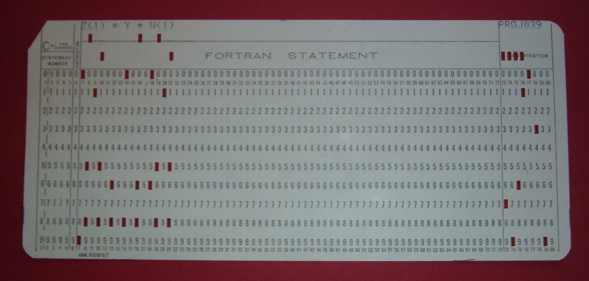
\includegraphics{images/chapter-1/perforated-card.png}
  \end{minipage}}
  \fbox{\begin{minipage}{\dimexpr \textwidth-2\fboxsep-2\fboxrule}
    \abovecaptionskip=0pt
    \caption{Perforated card}
  \end{minipage}}
\end{figure}

There are multiple lines on the card, each with varying holes. Each line describes a particular instruction that is necessary for the computations to be completed.

\begin{figure}[H]
  \lineskip=-\fboxrule
  \fbox{\begin{minipage}{\dimexpr \textwidth-2\fboxsep-2\fboxrule}
    \centering
    The user would describe their computations to someone who is capable of producing the correct perforated card needed for their computations.
    
	$\downarrow$
	
	The perforated card would be passed to the computer operator. A computer operator is a manager of computational resources that provides common services.
	
	$\downarrow$
	
	The computer operator would have a job queue from all of the users. These would be processed in a “first in, first out” (FIFO) fashion.
	
	$\downarrow$
	
	Jobs that are ready to be processed go in to batch processing. Each perforated card is passed through a computer system and the printed results are sent back to the user.
  \end{minipage}}
  \fbox{\begin{minipage}{\dimexpr \textwidth-2\fboxsep-2\fboxrule}
    \abovecaptionskip=0pt
    \caption{Process for performing computations in the 1950s}
  \end{minipage}}
\end{figure}


\section*{$>$1960s}

The process of performing computations after 1960 changed dramatically and required far less human input.

Automation was brought about by the “Operating System Paradigm” in which users could interface with a computer system directly through an operating system (OS).

\begin{figure}[H]
  \lineskip=-\fboxrule
  \fbox{\begin{minipage}{\dimexpr \textwidth-2\fboxsep-2\fboxrule}
    \centering
    \begin{tabular}{ccccc}
		User & $\rightarrow$ & Operating System (OS) & $\rightarrow$ & Results
	\end{tabular}
  \end{minipage}}
  \fbox{\begin{minipage}{\dimexpr \textwidth-2\fboxsep-2\fboxrule}
    \abovecaptionskip=0pt
    \caption{Process for performing computations after 1960}
  \end{minipage}}
\end{figure}


\section*{History details}

\begin{longtable}{|c|c|}
	\hline
	Late 1950s &
	\begin{minipage}[t]{0.8\textwidth}
    	\begin{itemize}
		    \item Standard subroutines were produced that were loaded at start-up. These contained features similar to those found on an operating system.
	  		\item Magnetic tapes were used for storage and were later replaced by disks.
	  		\item Assemblers started to be used. These are programs that takes basic computer instructions and convert them in to machine code; this is a pattern of binary bits (0’s and 1’s) that the computer system's processor can use to perform its basic operations.
	  		\item High-level languages, which consisted of more natural and human-readable language, started to be used. For example, FORTRAN is a general-purpose, compiled imperative programming language that is especially suited to numeric computation and scientific computing and was introduced in 1957.
    	\end{itemize}
  	\end{minipage}
	\\ \hline
	1960s &
	\begin{minipage}[t]{0.8\textwidth}
	  	Automated batch system.
	    \begin{itemize}
		    \item This replaced the computer operator.
		    \item Several programs could be loaded in to memory and automatically processed in a “first in, first out” (FIFO) fashion.
    	\end{itemize}
	\end{minipage}
	\\ \hline
	1970s &
	\begin{minipage}[t]{0.8\textwidth}
	  	Multiprogramming.
	    \begin{itemize}
		    \item The computer could switch between jobs, which allows processing and input/output (I/O) interaction simultaneously.
    	\end{itemize}
	\end{minipage}
	\\ \hline
	1980s &
	\begin{minipage}[t]{0.8\textwidth}
	  	Graphical user interfaces (GUIs).
	    \begin{itemize}
		    \item The interaction between a computer system and a user through the medium of a mouse and keyboard.
    	\end{itemize}
	\end{minipage}
	\\ \hline
\end{longtable}


\section{Hardware}

\section*{External hardware}

A \textbf{peripheral} is any external hardware device that provides input/output (I/O) for the computer.

For example, a keyboard and mouse are input peripherals, while a monitor and printer are output peripherals. Some peripherals, such as external hard drives, provide both input and output for the computer.

A computer system generally has many internal hardware components and hardware peripherals.

\begin{figure}[H]
  \lineskip=-\fboxrule
  \fbox{\begin{minipage}{\dimexpr \textwidth-2\fboxsep-2\fboxrule}
    \centering
    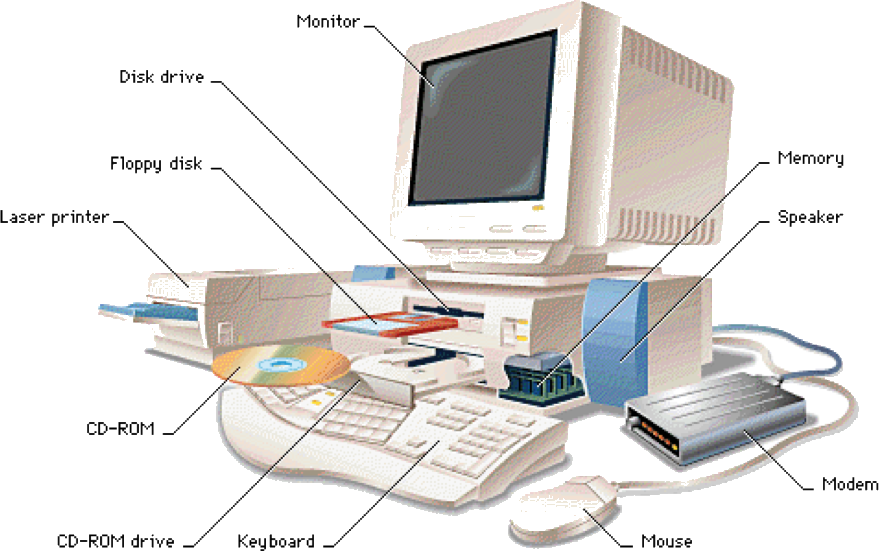
\includegraphics[max size={\textwidth}{\textheight}]{images/chapter-1/external-view-of-computer-system.png}
  \end{minipage}}
  \fbox{\begin{minipage}{\dimexpr \textwidth-2\fboxsep-2\fboxrule}
    \abovecaptionskip=0pt
    \caption{External view of computer system}
  \end{minipage}}
\end{figure}

\section*{Internal hardware}

A \textbf{processor} or \textbf{central processing unit (CPU)} is the hardware within a computer that carries out the instructions of a computer program by performing the basic arithmetical, logical, and input/output operations of the system.

A \textbf{motherboard} is the main printed circuit board (PCB) in a computer. The motherboard is a computer's central communications backbone connectivity point, through which all components and external peripherals connect.

Inside of a computer system, there are many components connected to the processor via the motherboard.

\begin{figure}[H]
  \lineskip=-\fboxrule
  \fbox{\begin{minipage}{\dimexpr \textwidth-2\fboxsep-2\fboxrule}
    \centering
    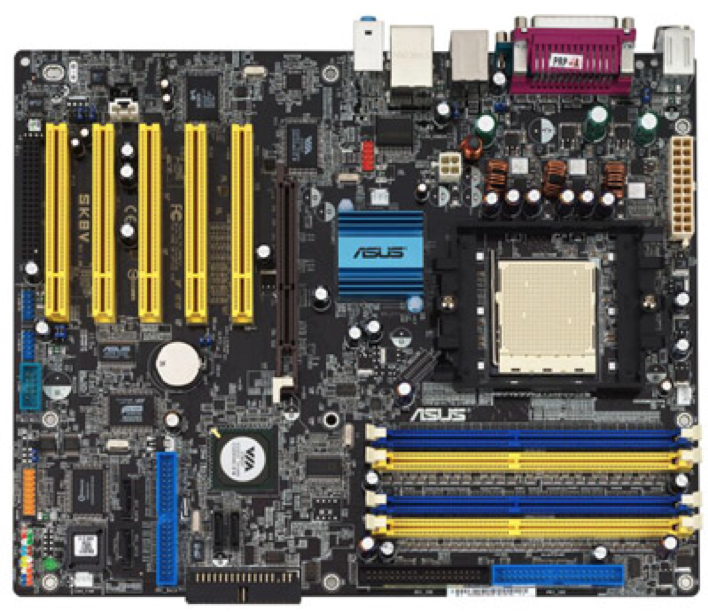
\includegraphics[max size={\textwidth}{\textheight}]{images/chapter-1/typical-computer-motherboard.png}
  \end{minipage}}
  \fbox{\begin{minipage}{\dimexpr \textwidth-2\fboxsep-2\fboxrule}
    \abovecaptionskip=0pt
    \caption{Typical computer motherboard}
  \end{minipage}}
\end{figure}

The motherboard connects:
\begin{itemize}
	\item all of the internal components via the data bus; and
	\item the peripherals.
\end{itemize}


\section{What is an operating system (OS)?}

\section*{Definition}

An \textbf{operating system (OS)} is a collection of system programs that manage the hardware resources and peripherals connected to a computer system. It is also responsible for the graphical user interface or command line interface and all other software running on the computer system.


\section*{Purpose of an operating system (OS)}

An operating system (OS) is designed to:
\begin{itemize}
	\item eliminate the need to have hardware knowledge to operate a computer system;
	\item make the boundary between hardware and software transparent, allowing the user to not be concerned with the technical details; and
	\item provide a user-friendly environment to execute and develop programs.
\end{itemize}

These attributes are achieved by layering the computer system such that the user can interface with applications, rather than the operating system (OS) or the hardware directly.

\begin{figure}[H]
  \lineskip=-\fboxrule
  \fbox{\begin{minipage}{\dimexpr \textwidth-2\fboxsep-2\fboxrule}
    \centering
    User
    
	$\updownarrow$
	
	Applications
	
	$\updownarrow$
	
	Operating System (OS)
	
	$\updownarrow$
	
	Computer System Hardware
  \end{minipage}}
  \fbox{\begin{minipage}{\dimexpr \textwidth-2\fboxsep-2\fboxrule}
    \abovecaptionskip=0pt
    \caption{Computer system layers}
  \end{minipage}}
\end{figure}


\section*{Structure of an operating system (OS)}

The structure of an operating system (OS) can be said to resemble an onion.

\begin{figure}[H]
  \lineskip=-\fboxrule
  \fbox{\begin{minipage}{\dimexpr \textwidth-2\fboxsep-2\fboxrule}
    \centering
    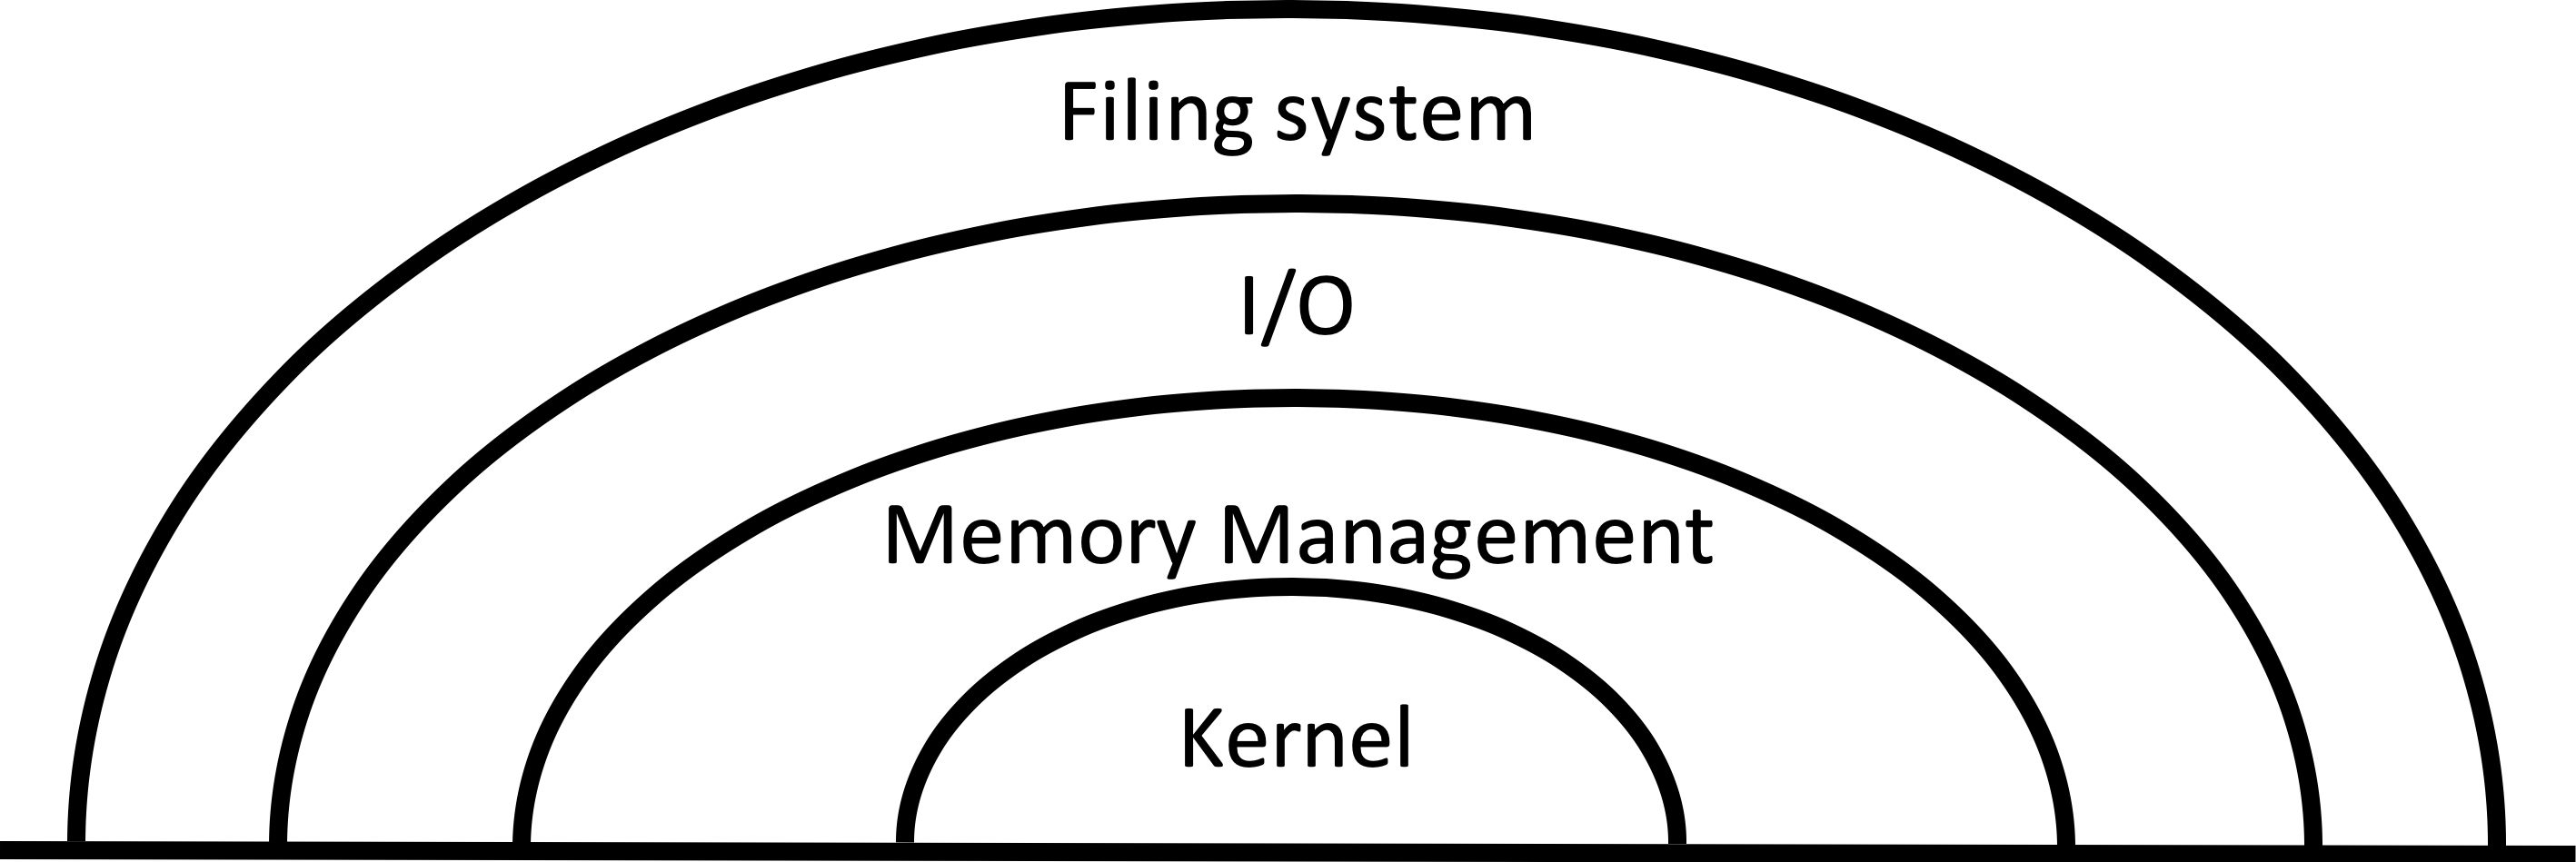
\includegraphics[max size={\textwidth}{\textheight}]{images/chapter-1/structure-of-an-os.png}
  \end{minipage}}
  \fbox{\begin{minipage}{\dimexpr \textwidth-2\fboxsep-2\fboxrule}
    \abovecaptionskip=0pt
    \caption{Structure of an operating system (OS)}
  \end{minipage}}
\end{figure}

An operating system (OS) has four main components.

The \textbf{kernel} hides the complexity of how a computer system works from users. It is responsible for:
\begin{itemize}
	\item process management;
	\item CPU scheduling; and
	\item handling interrupts.
\end{itemize}

\textbf{Memory management} is responsible for allocating and deallocating memory to processes.

\textbf{Input/output (I/O)} includes any interaction between the internal computer system components and peripherals.

The \textbf{filing system} is comprised of file management subsystems.

Each layer in the operating system (OS) structure provides functions to the above layers. Each layer uses facilities provided by layers within and below that layer. 


\section*{Practical features of current operating systems (OSs)}

\begin{longtable}{|c|c|}
	\hline
	Concurrency &
	\begin{minipage}[t]{0.6\textwidth}
	Allows overlapping input/output (I/O) operations with computations and several programs to be stored in memory at a single time.
	\end{minipage}
	\\ \hline
	Sharing of resources &
	\begin{minipage}[t]{0.6\textwidth}
	Sharing hardware and peripherals, such as hard disks and printers.
	\end{minipage}
	\\ \hline
	Access to long term storage &
	\begin{minipage}[t]{0.6\textwidth}
	Important for saving important files on mediums such as hard disk drives (HDDs) and solid-state drives (SSDs).
	\end{minipage}
	\\ \hline
	Non-determinacy &
	\begin{minipage}[t]{0.6\textwidth}
	The ability to cope with unpredictable events without crashing.
	\end{minipage}
	\\ \hline
\end{longtable}


\section{Functions of an operating system}

An operating system (OS) has two main complementary functions:
\begin{itemize}
	\item resource managing; and
	\item machine extending.
\end{itemize}


\section*{Resource managing}

It manages resources shared among users and user programs and maximises their utilisation of the CPU, RAM and other resources. This is done simultaneously in order to increase the availability.

This is similar to the role of computer operators in the 1950s.


\section*{Machine extending}

It presents a virtual machine (or extended machine) to users that is much easier to access than the underlying physical machine.

\begin{figure}[H]
  \lineskip=-\fboxrule
  \fbox{\begin{minipage}{\dimexpr \textwidth-2\fboxsep-2\fboxrule}
    \centering
    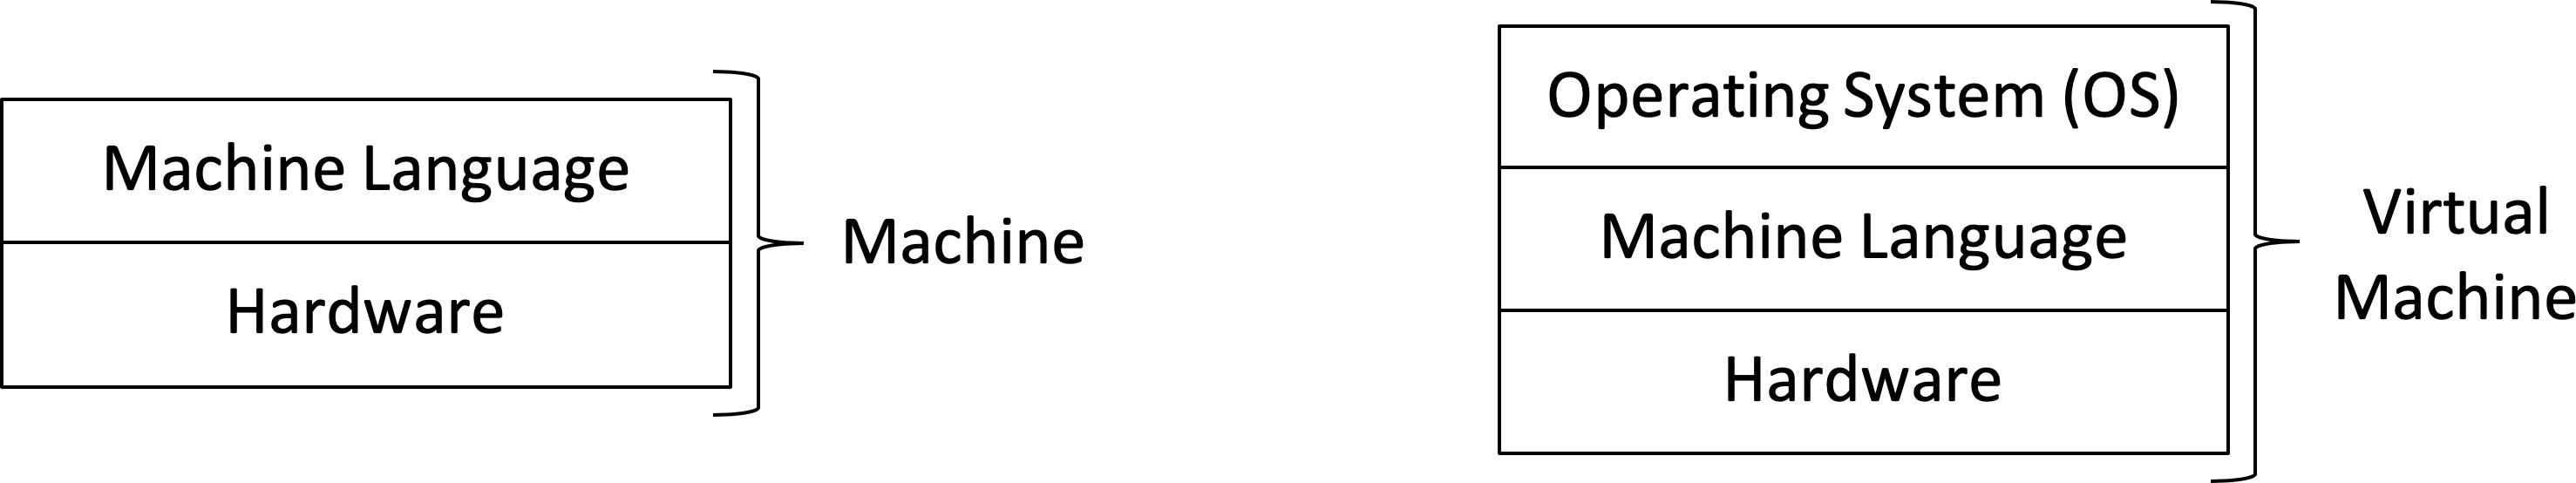
\includegraphics[max size={\textwidth}{\textheight}]{images/chapter-1/machine-extending.png}
  \end{minipage}}
  \fbox{\begin{minipage}{\dimexpr \textwidth-2\fboxsep-2\fboxrule}
    \abovecaptionskip=0pt
    \caption{Machine extending}
  \end{minipage}}
\end{figure}

The virtual machine presented to the user provides an abstraction of the computer system. This hides the complexity of the hardware from the user; this means that the user need only be concerned with the details of the hardware if they desire.

This is a way of translating the functions needed by a user from the hardware to a presentable and user-friendly medium. As a result, the operating system (OS) acts as an intermediary layer between the user and machine language.

The benefit of this abstraction can be demonstrated when comparing how computations may be processed with and without an operating system (OS).

\begin{figure}[H]
  \lineskip=-\fboxrule
  \fbox{\begin{minipage}{\dimexpr \textwidth-2\fboxsep-2\fboxrule}
    \begin{longtable}{|c|c|}
    	\hline
		\textbf{Without Operating System (OS)} & \textbf{With Operating System (OS)} \\
		\hline
		\begin{minipage}[t]{0.45\textwidth}
	    	The instructions written in machine code or assembly language much interface directly with memory hardware. As such, the memory locations to load the two numbers from must be explicitly defined and the memory location to which the result is stored must also be defined.
	    	
			The example below shows a possible assembly code implementation of a computation that is capable of adding two numbers.
	  	\end{minipage}
		&
		\begin{minipage}[t]{0.45\textwidth}
	    	The instructions can be written in a high-level language, such as C++.
	  	\end{minipage}
		\\ \hline
		\begin{minipage}[t]{0.45\textwidth}
			\begin{tabular}{p{2cm} | p{3.5cm}}
				\hline
				LDAA \$80 & (load number at memory location 80) \\
				\hline
				LDAB \$81 & (load number at memory location 81) \\
				\hline
				ADDB & (add these two numbers) \\
				\hline
				STAA \&55 & (store the sum to memory location 55) \\
				\hline
			\end{tabular}
	  	\end{minipage}
		&
		\begin{minipage}[t]{0.45\textwidth}
	    	int a, b, c;
	    	
			a = 1;
			
			b = 2;
			
			c = a + b;
	  	\end{minipage}
	\end{longtable}
	
  \end{minipage}}
  \fbox{\begin{minipage}{\dimexpr \textwidth-2\fboxsep-2\fboxrule}
    \abovecaptionskip=0pt
    \caption{Adding two numbers}
  \end{minipage}}
\end{figure}

This demonstrates that program development is much more user-friendly with an operating system (OS). This is because without an operating system (OS) the user must have knowledge of the system hardware; in this case, the necessary memory locations.

In addition, it is possible that the machine code or assembly language written may not work on another computer system as that computer system may have a different architecture or the memory locations may be different. For example, in another computer system:
\begin{itemize}
	\item memory location 81 may not exist as the memory is smaller; or
	\item memory location 55 contains important data or instructions that should not be overwritten and therefore the computer system may crash.
\end{itemize}

By contrast, with an operating system (OS), it is possible to perform computations without interfacing directly with hardware. In the example above, variables (a, b and c) can be used to access data in memory rather than addressing memory locations. The only concern here is that the variable c is able to store the result of a + b.

The operating system (OS) provides a unified environment to users to run their computations in different systems. The operating system (OS) is capable of taking high-level code and translating it in to the machine code that can be executed on a particular computer system.


\section{Current operating system (OS) trends}

\section*{Hardware evolution}

Due to fast rate of hardware evolution, operating systems (OSs) are more wide-spread than just traditional desktop computers. They can be found on hardware such as:
\begin{itemize}
	\item mobile devices, such as smartphones and tablets; and
	\item embedded systems.
\end{itemize}

\begin{figure}[H]
  \lineskip=-\fboxrule
  \fbox{\begin{minipage}{\dimexpr \textwidth-2\fboxsep-2\fboxrule}
    \begin{longtable}{|c|c|c|}
    	\hline
		\textbf{Desktop} & \textbf{Mobile} & \textbf{Embedded} \\
		\hline
		\begin{minipage}[t]{0.26\textwidth}
	    	\begin{itemize}
	    		\item Windows
	    		\item macOS
	    		\item Linux
	    	\end{itemize}
	  	\end{minipage}
		&
		\begin{minipage}[t]{0.26\textwidth}
	    	\begin{itemize}
	    		\item iOS
	    		\item Android
	    		\item Symbian OS
	    	\end{itemize}
	  	\end{minipage}
		&
		\begin{minipage}[t]{0.26\textwidth}
	    	\begin{itemize}
	    		\item Windows Embedded
	    	\end{itemize}
	  	\end{minipage}
	  	\\ \hline
	\end{longtable}
  \end{minipage}}
  \fbox{\begin{minipage}{\dimexpr \textwidth-2\fboxsep-2\fboxrule}
    \abovecaptionskip=0pt
    \caption{Popular operating systems (OSs)}
  \end{minipage}}
\end{figure}


\section*{Multiprocessor systems}

\subsection*{Definiton}

A \textbf{multiple processor computer system} makes use of two or more processors and has the ability to allocate tasks between them.


\subsection*{Workstations}

A single machine may contain multiple processors and therefore have large computing power.


\subsection*{Distributed and network systems}

These computer systems share computing power and peripherals.

\begin{figure}[H]
  \lineskip=-\fboxrule
  \fbox{\begin{minipage}{\dimexpr \textwidth-2\fboxsep-2\fboxrule}
    \centering
    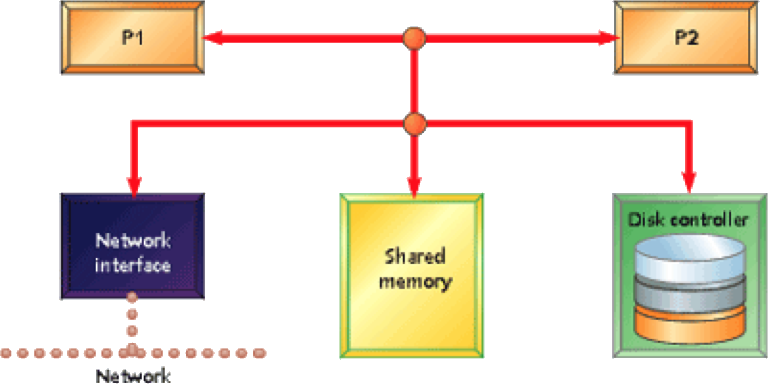
\includegraphics[max size={\textwidth}{\textheight}]{images/chapter-1/distributed-and-network-systems.png}
  \end{minipage}}
  \fbox{\begin{minipage}{\dimexpr \textwidth-2\fboxsep-2\fboxrule}
    \abovecaptionskip=0pt
    \caption{Distributed and network systems}
  \end{minipage}}
\end{figure}

The diagram shows an abstraction of a distributed or network system. P1 and P2 are the connected computer systems that both share memory, access to the disk control and, if the system is a network system, the network interface.

However, there is a distinguishable difference between distributed and network systems.

\begin{longtable}{|c|c|}
	\hline
	\textbf{Similarities} & \textbf{Differences} \\
	\hline
	\begin{minipage}[t]{0.45\textwidth}
		Consist of multiple systems that are interconnected to exchange information.
	\end{minipage}
	&
	\begin{minipage}[t]{0.45\textwidth}
		In distributed systems, users are not aware of the multiplicity of computer systems available.
	\end{minipage}
	\\ \hline
	&
	\begin{minipage}[t]{0.45\textwidth}
		In network systems, users explicitly move/share files, submit jobs for processing and other perform other similar tasks.
	\end{minipage}
	\\ \hline
	&
	\begin{minipage}[t]{0.45\textwidth}
		In distributed systems, tasks such as moving/sharing files, submitting jobs for processing and other similar tasks are handled automatically by the operating system (OS).
	\end{minipage}
	\\ \hline
\end{longtable}


\subsection*{Evaluation}

\begin{longtable}{|c|c|}
	\hline
	\textbf{Advantages} & \textbf{Disadvantages} \\
	\hline
	\begin{minipage}[t]{0.45\textwidth}
		\textbf{Increase processor throughput} due to the use of parallel processing.
	\end{minipage}
	&
	\begin{minipage}[t]{0.45\textwidth}
		\textbf{A more complex operating system is required} in order to be able to interface and manage multiple processor units.
	\end{minipage}
	\\ \hline
	\begin{minipage}[t]{0.45\textwidth}
		\textbf{Lower cost} than using multiple processors across multiple computer systems because the processors share resources such as the power supply and motherboard.
	\end{minipage}
	&
	\\ \hline
	\begin{minipage}[t]{0.45\textwidth}
		\textbf{Increased reliability} because failure of one processor does not affect the other processors and will only slow down the computer system.
	\end{minipage}
	&
	\\ \hline
\end{longtable}


\section{Operating system (OS) layers}

\section*{User interfaces}

In an operating system (OS), the top layer is the user interface. This is the only layer explicitly visible to the user.

The user interface may be a:
\begin{longtabu} to \textwidth {X[6,l] X[1,c] X[10,l]}
	\textbullet terminal & -- & text-based command prompt; and/or
	\\
	\textbullet graphical user interface (GUI) & -- & a visual way of interacting with a computer using items such as windows, icons and menus.
\end{longtabu}


\subsection*{History of the graphical user interface (GUI)}

The first company to develop a graphical user interface (GUI) was Xerox PARC. They developed the “Alto” personal computer. It had a bitmapped screen and was the first computer to have a “desktop” screen with a graphical user interface (GUI).

The “Alto” personal computer was not a commercial product. However, several thousand units were manufactured and used at Xerox’s offices and several universities.

This development was a large influence on the design of personal computers during the late 1970s and early 1980s. Notable examples include:
\begin{itemize}
	\item Three Rivers PERQ;
	\item Apple Lisa;
	\item Apple Macintosh; and
	\item the first Sun Workstations.
\end{itemize}


\section{Kernel mode}

\section*{Kernel mode vs user mode}

\begin{longtabu} to \textwidth {| X[1,l] | X[1,l] |}
    \hline
    \textbf{Kernel Mode} & \textbf{User Mode}
    \\ \hline
    Operating systems (OSs) run in kernel mode.
    
    This allows:
    \begin{itemize}
    	\item execution of privileged machine instructions; and
    	\item complete access and control of all the hardware.
    \end{itemize}
    &
    Other software runs in user mode.

	In this mode, instructions that affect control of the machine are forbidden.

	For example:
	\begin{itemize}
		\item 	web browsers;
		\item e-mail software; and
		\item music players.
	\end{itemize}
	\\ \hline
\end{longtabu}

\begin{figure}[H]
  \lineskip=-\fboxrule
  \fbox{\begin{minipage}{\dimexpr \textwidth-2\fboxsep-2\fboxrule}
    \centering
    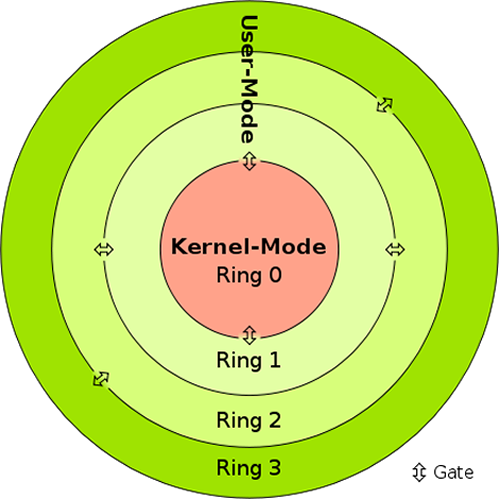
\includegraphics[max size={\textwidth}{\textheight}]{images/chapter-1/kernel-mode-and-user-mode.png}
  \end{minipage}}
  \fbox{\begin{minipage}{\dimexpr \textwidth-2\fboxsep-2\fboxrule}
    \abovecaptionskip=0pt
    \caption{Kernel mode and user mode}
  \end{minipage}}
\end{figure}

Ring 0 represents the kernel mode.

Rings 1-3 represent the user mode.


\section*{Kernel mode protection}

These rings allow separation between the operating system (OS) and user programs for security and protection purposes.

If user mode had unrestricted access to all of the machine instructions:
\begin{itemize}
	\item a user could inadvertently obtain a virus or write code that is capable of causing damage to the system, and therefore it is necessary to prevent any instructions from directly controlling the machine;
	\item a program may use resources unfairly, such as holding the CPU or memory, and therefore harm the execution of other programs; and/or
	\item sensitive machine instructions could be used improperly which may lead to kernel mode errors.
\end{itemize}

Kernel mode errors are catastrophic.


\begin{figure}[H]
  \lineskip=-\fboxrule
  \fbox{\begin{minipage}{\dimexpr \textwidth-2\fboxsep-2\fboxrule}
    \begin{longtabu} to \textwidth {| X[1,l] | X[1,l] |}
	    \hline
	    \textbf{Kernel Mode} & \textbf{User Mode}
	    \\ \hline
	    A kernel panic represents the operating system (OS) attempting to prevent software causing any harm to the computer system and to recover from a kernel mode error on reboot.
	    
	    An example of a kernel panic is the “Blue Screen of Death” (BSoD) in Microsoft’s Windows.
	    &
	    Application errors where an exception was thrown due to an attempt to execute a privileged instruction, this is one that should only be accessed and executed by the kernel mode, represents the operating system (OS) preventing an application from having unrestricted access to all of the machine instructions.
		\\ \hline
		\centering
    	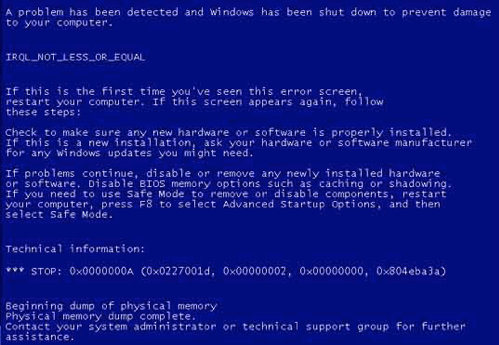
\includegraphics[max size={0.45\textwidth}{\textheight}]{images/chapter-1/kernel-mode-error-bsod.png}
	    &
	    \centering
    	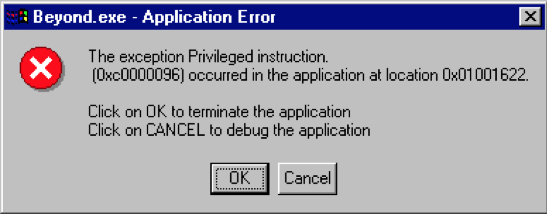
\includegraphics[max size={0.45\textwidth}{\textheight}]{images/chapter-1/kernel-mode-error-application-error.png}
		\\ \hline
	\end{longtabu}
  \end{minipage}}
  \fbox{\begin{minipage}{\dimexpr \textwidth-2\fboxsep-2\fboxrule}
    \abovecaptionskip=0pt
    \caption{Kernel mode errors}
  \end{minipage}}
\end{figure}


\section*{System calls}

A \textbf{system call} is the programmatic way in which a computer program requests a service from the kernel of the operating system on which it is executed. A system call is a way for programs to interact with the operating system.

Some privileged instructions can be called by a programmer via system calls. Operating systems (OSs) contain system calls for which provide a layer of services for user programs to implement some activities/request services. These are usually sensitive or privileged from the kernel.

All interactions with the hardware are implemented via system calls. For example, a system call may occur if an application requires interaction with a peripheral such as a printer.

Invoking a system call is similar to calling a general function. However, the difference is that a general function’s code is part of program itself, while the system call code is part of the operating system (OS). Different operating systems (OSs) offer different (limited) sets of system calls.

\begin{figure}[H]
  \lineskip=-\fboxrule
  \fbox{\begin{minipage}{\dimexpr \textwidth-2\fboxsep-2\fboxrule}
    \begin{longtabu} to \textwidth {| X[1,l] | X[2,l] |}
	    \hline
	    \textbf{Call} & \textbf{Description}
	    \\ \hline
	    \multicolumn{2}{|c|}{\textbf{Process Mangament}}
	    \\ \hline
	    pid = fork()
	    &
	    Create a child process identical to the parent.
		\\ \hline
		exit(status)
	    &
	    Terminate process execution and return status.
		\\ \hline
		\multicolumn{2}{|c|}{\textbf{File Mangament}}
	    \\ \hline
	    n = read(fd, buffer, nbytes)
	    &
	    Read data from a file in to a buffer.
		\\ \hline
		n = write(fd, buffer, nbytes)
	    &
	    Write data to a file
		\\ \hline
		\multicolumn{2}{|c|}{\textbf{Process Mangament}}
	    \\ \hline
	    seconds = time(\&seconds)
	    &
	    Get the elapsed time since Jan 1. 1970
		\\ \hline
	\end{longtabu}
  \end{minipage}}
  \fbox{\begin{minipage}{\dimexpr \textwidth-2\fboxsep-2\fboxrule}
    \abovecaptionskip=0pt
    \caption{Unix system calls}
  \end{minipage}}
\end{figure}


\chapter{Process Management}

\section{Programs and processes}

\section*{Definitions}

A \textbf{program} is the code written by a programmer.

A \textbf{process} (or job/task) shows a program in execution and is a particular instance of a program. These many be shown in a monitoring software, such as Windows Task Manager.

\textbf{Data} are stored values used for the computations by the process.


\section*{How it works}

A single program may have multiple processes that are currently running.

Each process can share the same code for the program. This is possible as each process uses its own address space, a list of memory locations which the process can read and write. These memory locations contain the program’s code instructions and data.

A program is only code however, once it is run, a process is started, and it becomes instructions and data.

\begin{figure}[H]
  \lineskip=-\fboxrule
  \fbox{\begin{minipage}{\dimexpr \textwidth-2\fboxsep-2\fboxrule}
    \centering
    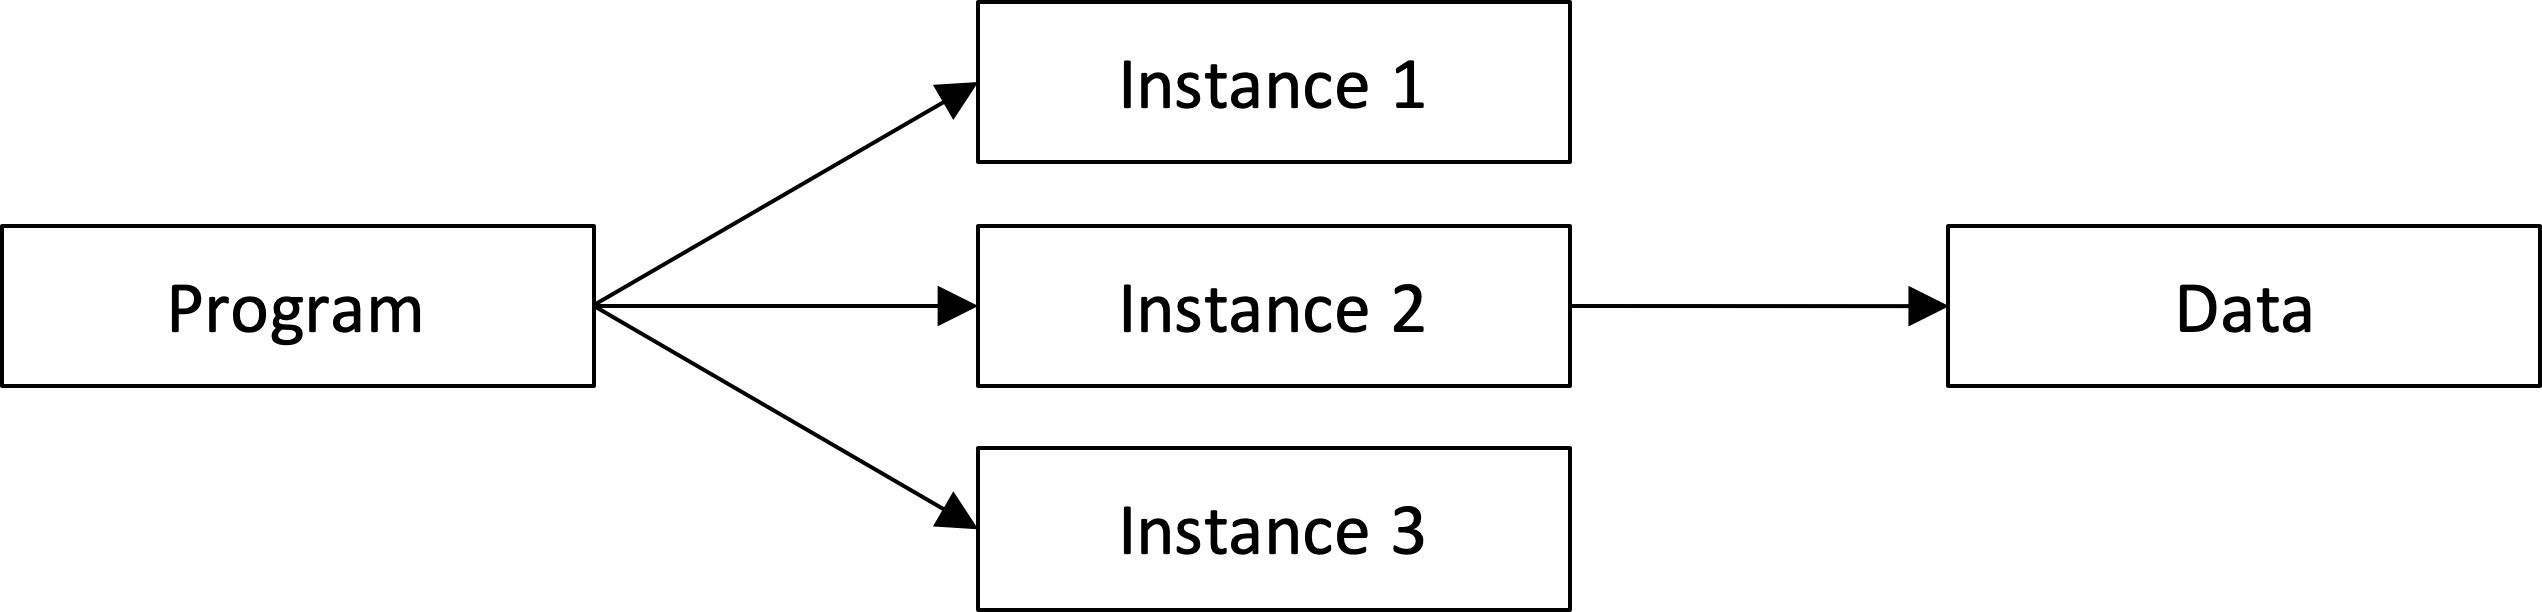
\includegraphics[max size={\textwidth}{\textheight}]{images/chapter-2/programs-and-processes.png}
  \end{minipage}}
  \fbox{\begin{minipage}{\dimexpr \textwidth-2\fboxsep-2\fboxrule}
    \abovecaptionskip=0pt
    \caption{Programs and processes}
  \end{minipage}}
\end{figure}


\section{Process life cycle}

\section*{Process creation}

A process can be created by:

\begin{longtabu} to \textwidth {X[3,l] X[1,c] X[10,l]}
	\textbullet a user & -- & a program may be executed by a user, such as via a double-click using a graphical user interface (GUI) or by typing in a command, and “trigger” the processor to load the program’s executable file containing the program code; or
	\\
	\textbullet another process & -- & an existing process may create another process by spawning/forking – the process that creates a new process is called the parent process while the new process is called the child process. The child process may also spawn a new process forming a tree of processes, as demonstrated in the diagram below.
\end{longtabu}

\begin{figure}[H]
  \lineskip=-\fboxrule
  \fbox{\begin{minipage}{\dimexpr \textwidth-2\fboxsep-2\fboxrule}
    \centering
    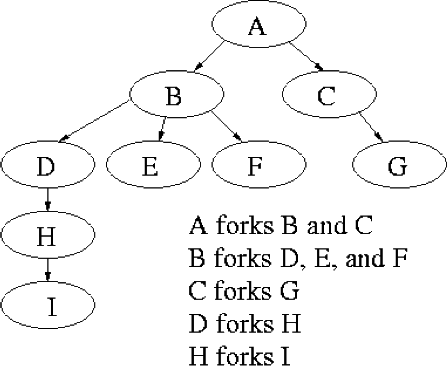
\includegraphics[max size={\textwidth}{\textheight}]{images/chapter-2/process-creation.png}
  \end{minipage}}
  \fbox{\begin{minipage}{\dimexpr \textwidth-2\fboxsep-2\fboxrule}
    \abovecaptionskip=0pt
    \caption{Process creation}
  \end{minipage}}
\end{figure}


\section*{Process table and process control block}

A \textbf{process identification number (PID)} is a unique identifier given to a new process when it is created.

A \textbf{process control block (PCB)} holds all of the information about a process. It is created when new process is created.

A \textbf{process table} stores the process identification numbers (PIDs) for a process and a pointer to the respective process control block (PCB) for that process. This is managed by the operating system (OS).

\begin{figure}[H]
  \lineskip=-\fboxrule
  \fbox{\begin{minipage}{\dimexpr \textwidth-2\fboxsep-2\fboxrule}
    \centering
    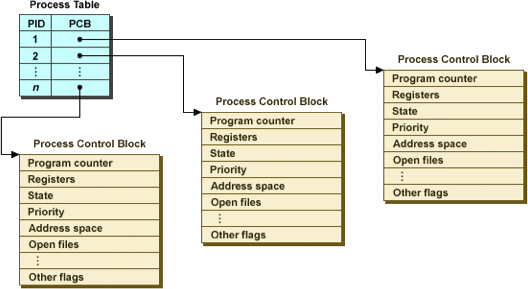
\includegraphics[max size={\textwidth}{\textheight}]{images/chapter-2/process-table.png}
  \end{minipage}}
  \fbox{\begin{minipage}{\dimexpr \textwidth-2\fboxsep-2\fboxrule}
    \abovecaptionskip=0pt
    \caption{Process table with respective process control blocks}
  \end{minipage}}
\end{figure}

The process descriptor fields in the process control block (PCB) may differ between operating system (OS). An example of possible process descriptor fields is shown by those used by the Minix operating system (OS) are shown below.

\begin{figure}[H]
  \lineskip=-\fboxrule
  \fbox{\begin{minipage}{\dimexpr \textwidth-2\fboxsep-2\fboxrule}
    \begin{longtabu} to \textwidth {X[2,l] X[2,l] X[2,l]}
	    \hline
	    \textbf{Process Management} & \textbf{Memory Management} & \textbf{File Management}
	    \\ \hline
	    Registers & Pointer to text segment	& UMASK mask
		\\ \hline
		Program counter & Pointer to data segment & Root directory
		\\ \hline
		Program status word & Pointer to bss segment & Working directory
		\\ \hline
		Stack pointer & Exit status & File descriptors
		\\ \hline
		Process state & Signal status & Effective uid
		\\ \hline
		Time when process started & Process ID & Effective gid
		\\ \hline
		CPU time used & Parent process & System call parameters
		\\ \hline
		Children’s CPU time & Process group & Various flag bits
		\\ \hline
		Time of next alarm & Real uid &
		\\ \hline
		Message queue pointers & Effective uid &
		\\ \hline
		Pending signal bits & Real gid &
		\\ \hline
		Process ID & Effective gid &
		\\ \hline
		Various flag bits & Various flag bits &
		\\ \hline
	\end{longtabu}
  \end{minipage}}
  \fbox{\begin{minipage}{\dimexpr \textwidth-2\fboxsep-2\fboxrule}
    \abovecaptionskip=0pt
    \caption{Process descriptor fields in Minix}
  \end{minipage}}
\end{figure}

Although Minix is a fully-featured operating system (OS), it is a small operating system (OS) and therefore the processor descriptor fields are less complex than other operating systems (OSs).


\section*{Three-state model}

The \textbf{three-state model} shows how a process, once initiated, can be in one of three states. The current state of a process is stored in its respective process control block (PCB).

A process, once initiated, can be in one of three main states:
\begin{longtabu} to \textwidth {X[2,l] X[1,c] X[10,l]}
	\textbullet running & -- & actually using the CPU to perform a task;
	\\
	\textbullet ready & -- & ready to run but waiting for the CPU as it has not yet had time on the CPU has been temporarily stopped to let another process run; or
	\\
	\textbullet ready & -- & unable to run until some external event occurs, such as:
		\begin{itemize}
			\item waiting for an interrupt, this is a message from the hardware saying that a resource is now available to read from – such as waiting for an input/output (I/O) operation to complete; and
			\item waiting for another process to finish accessing a shared resources – for example: a file; memory; or an external peripheral, such as a printer.
		\end{itemize}
\end{longtabu}

\begin{figure}[H]
  \lineskip=-\fboxrule
  \fbox{\begin{minipage}{\dimexpr \textwidth-2\fboxsep-2\fboxrule}
    \centering
    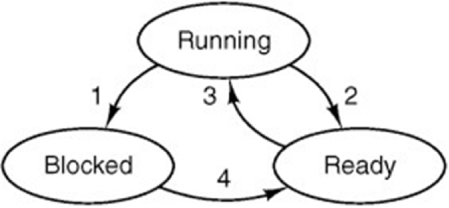
\includegraphics[max size={\textwidth}{\textheight}]{images/chapter-2/process-states.png}
  \end{minipage}}
  \fbox{\begin{minipage}{\dimexpr \textwidth-2\fboxsep-2\fboxrule}
    \abovecaptionskip=0pt
    \caption{Process states}
  \end{minipage}}
\end{figure}

In reference to the diagram above, transitions can occur between process states.

\begin{figure}[H]
  \lineskip=-\fboxrule
  \fbox{\begin{minipage}{\dimexpr \textwidth-2\fboxsep-2\fboxrule}
    \begin{longtabu} to \textwidth {|X[4,l]|X[1.5,l]|X[6,l]|}
	    \hline
	    \textbf{Transition} & \textbf{Diagram Number} & \textbf{Explanation}
	    \\ \hline
	    \textbf{running $\rightarrow$ blocked}
	    & \textbf{1} &
	    \textbf{Process blocks for input.}
	    
		For example, if the process is waiting for some input from I/O.
		\\ \hline
		\textbf{running $\rightarrow$ ready}
	    & \textbf{2} &
	    \textbf{Scheduler picks another process.}
	    
		The process has had opportunity to run and is flagged as no longer currently running, so that another process can run.
		\\ \hline
		\textbf{ready $\rightarrow$ running}
	    & \textbf{3} &
	    \textbf{Scheduler picks this process.}
		The next process that is ready to run is set to running to allow access to the CPU.
		\\ \hline
		\textbf{blocked $\rightarrow$ ready}
	    & \textbf{4} &
	    \textbf{Input becomes available.}
		The process has received input from I/O or the process sends an interrupt and the interrupt service routine (ISR) is executed, the scheduler is called to transition the process from blocked to ready.
		\\ \hline
	\end{longtabu}
  \end{minipage}}
  \fbox{\begin{minipage}{\dimexpr \textwidth-2\fboxsep-2\fboxrule}
    \abovecaptionskip=0pt
    \caption{Transitions between processor states}
  \end{minipage}}
\end{figure}

The transition between process states is dependent on the scheduling algorithm used. A clock is used to send a signal to stop the current process, move it from running to ready and then run the scheduler to find out what process should be processed next and the next process will be made to running.


\section*{State queues}

At any time, a process is in only one state.


\subsection*{Running processes}

At any time, at most one process is in the running state. This is because a single-core processor is only able to process one instruction coming from a single core at a time. If a computer system has a multi-core processor, this rule applies to each individual core on the processor, rather than the processor as a whole, as they are able to complete parallel execution.

\begin{figure}[H]
  \lineskip=-\fboxrule
  \fbox{\begin{minipage}{\dimexpr \textwidth-2\fboxsep-2\fboxrule}
    \centering
    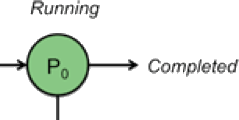
\includegraphics[max size={\textwidth}{\textheight}]{images/chapter-2/running-processes.png}
  \end{minipage}}
  \fbox{\begin{minipage}{\dimexpr \textwidth-2\fboxsep-2\fboxrule}
    \abovecaptionskip=0pt
    \caption{Running processes}
  \end{minipage}}
\end{figure}


\subsection*{Ready processes}

There may be a queue of processes in the ready state.

\begin{figure}[H]
  \lineskip=-\fboxrule
  \fbox{\begin{minipage}{\dimexpr \textwidth-2\fboxsep-2\fboxrule}
    \centering
    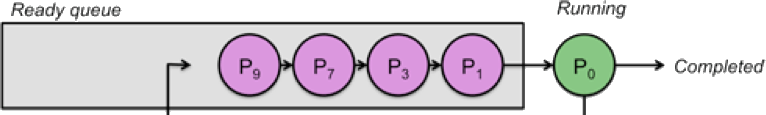
\includegraphics[max size={\textwidth}{\textheight}]{images/chapter-2/ready-processes.png}
  \end{minipage}}
  \fbox{\begin{minipage}{\dimexpr \textwidth-2\fboxsep-2\fboxrule}
    \abovecaptionskip=0pt
    \caption{Ready processes}
  \end{minipage}}
\end{figure}


\subsection*{Blocked processes}

There may be several queues of processes in the blocked state, where each queue represents one resource for which processes in that queue are waiting.

\begin{figure}[H]
  \lineskip=-\fboxrule
  \fbox{\begin{minipage}{\dimexpr \textwidth-2\fboxsep-2\fboxrule}
    \centering
    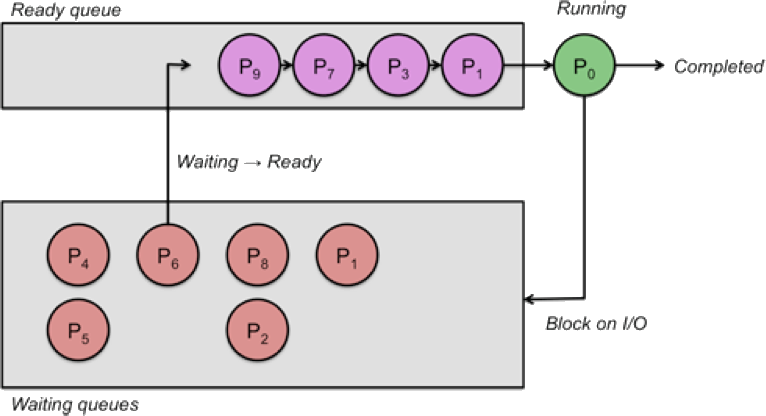
\includegraphics[max size={\textwidth}{\textheight}]{images/chapter-2/currently-running-processes.png}
  \end{minipage}}
  \fbox{\begin{minipage}{\dimexpr \textwidth-2\fboxsep-2\fboxrule}
    \abovecaptionskip=0pt
    \caption{Currently running processes}
  \end{minipage}}
\end{figure}


\section*{Process termination}

\textbf{Process termination} is the end of life for a process, this can occur in two general ways.


\subsection*{Voluntary termination}

\textbf{Voluntary termination} of a process represents the end of life for a process where its termination was intended by the user or the programmer.

This can be a:
\begin{longtabu} to \textwidth { X[1.5,l] X[0.2,l] X[7,l]}
	\textbf{\textbullet normal exit}
	& -- &
	the process has done its work; or
	\\
	\textbf{\textbullet error exit}
	& -- &
	the process itself handles and “catches” an error – for example, some try-catch code is implemented to check if a condition is met, such as if the definition of a variable is present.
\end{longtabu}

\begin{figure}[H]
  \lineskip=-\fboxrule
  \fbox{\begin{minipage}{\dimexpr \textwidth-2\fboxsep-2\fboxrule}
    \centering
    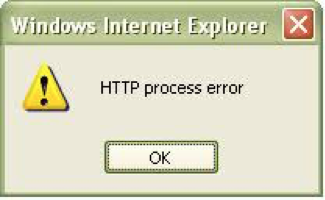
\includegraphics[max size={\textwidth}{\textheight}]{images/chapter-2/voluntary-termination.png}
  \end{minipage}}
  \fbox{\begin{minipage}{\dimexpr \textwidth-2\fboxsep-2\fboxrule}
    \abovecaptionskip=0pt
    \caption{Voluntary termination due to an error exit}
  \end{minipage}}
\end{figure}


\subsection*{Involuntary termination}

\textbf{Involuntary termination} of a process represents the end of life for a process where its termination as not intended by the user or the programmer.

This can be due to:
\begin{longtabu} to \textwidth { X[1.5,l] X[0.2,l] X[7,l]}
	\textbf{\textbullet a fatal error}
	& -- &
	an error is detected by the operating system’s (OS’s) protected mode – for example, an exception has been thrown due to reference to a non-existent memory location or division by zero; or
	\\
	\textbf{\textbullet being killed by another process}
	& -- &
	a process may execute a system call that causes the operating system (OS) to kill another process – this process may have control over the killed process and this may be due to that process being the parent process of the killed process.
\end{longtabu}

\begin{figure}[H]
  \lineskip=-\fboxrule
  \fbox{\begin{minipage}{\dimexpr \textwidth-2\fboxsep-2\fboxrule}
    \centering
    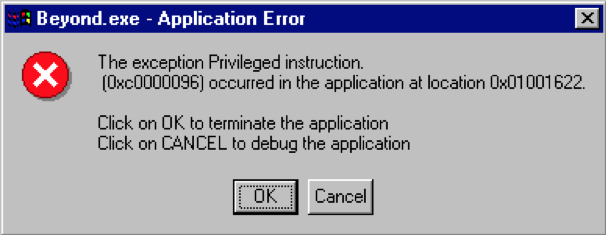
\includegraphics[max size={\textwidth}{\textheight}]{images/chapter-2/involuntary-termination.png}
  \end{minipage}}
  \fbox{\begin{minipage}{\dimexpr \textwidth-2\fboxsep-2\fboxrule}
    \abovecaptionskip=0pt
    \caption{Voluntary termination due to an error exit}
  \end{minipage}}
\end{figure}


\newpage
\section{Program execution}

\section*{The simple fetch-execute cycle}

\subsection*{Definition}

The \textbf{fetch-execute cycle} is an operational process in which a computer system retrieves a program instruction from its memory, determines what actions the instruction dictates, and carries out those actions.


\subsection*{How it works}

\begin{figure}[H]
  \lineskip=-\fboxrule
  \fbox{\begin{minipage}{\dimexpr \textwidth-2\fboxsep-2\fboxrule}
    \centering
    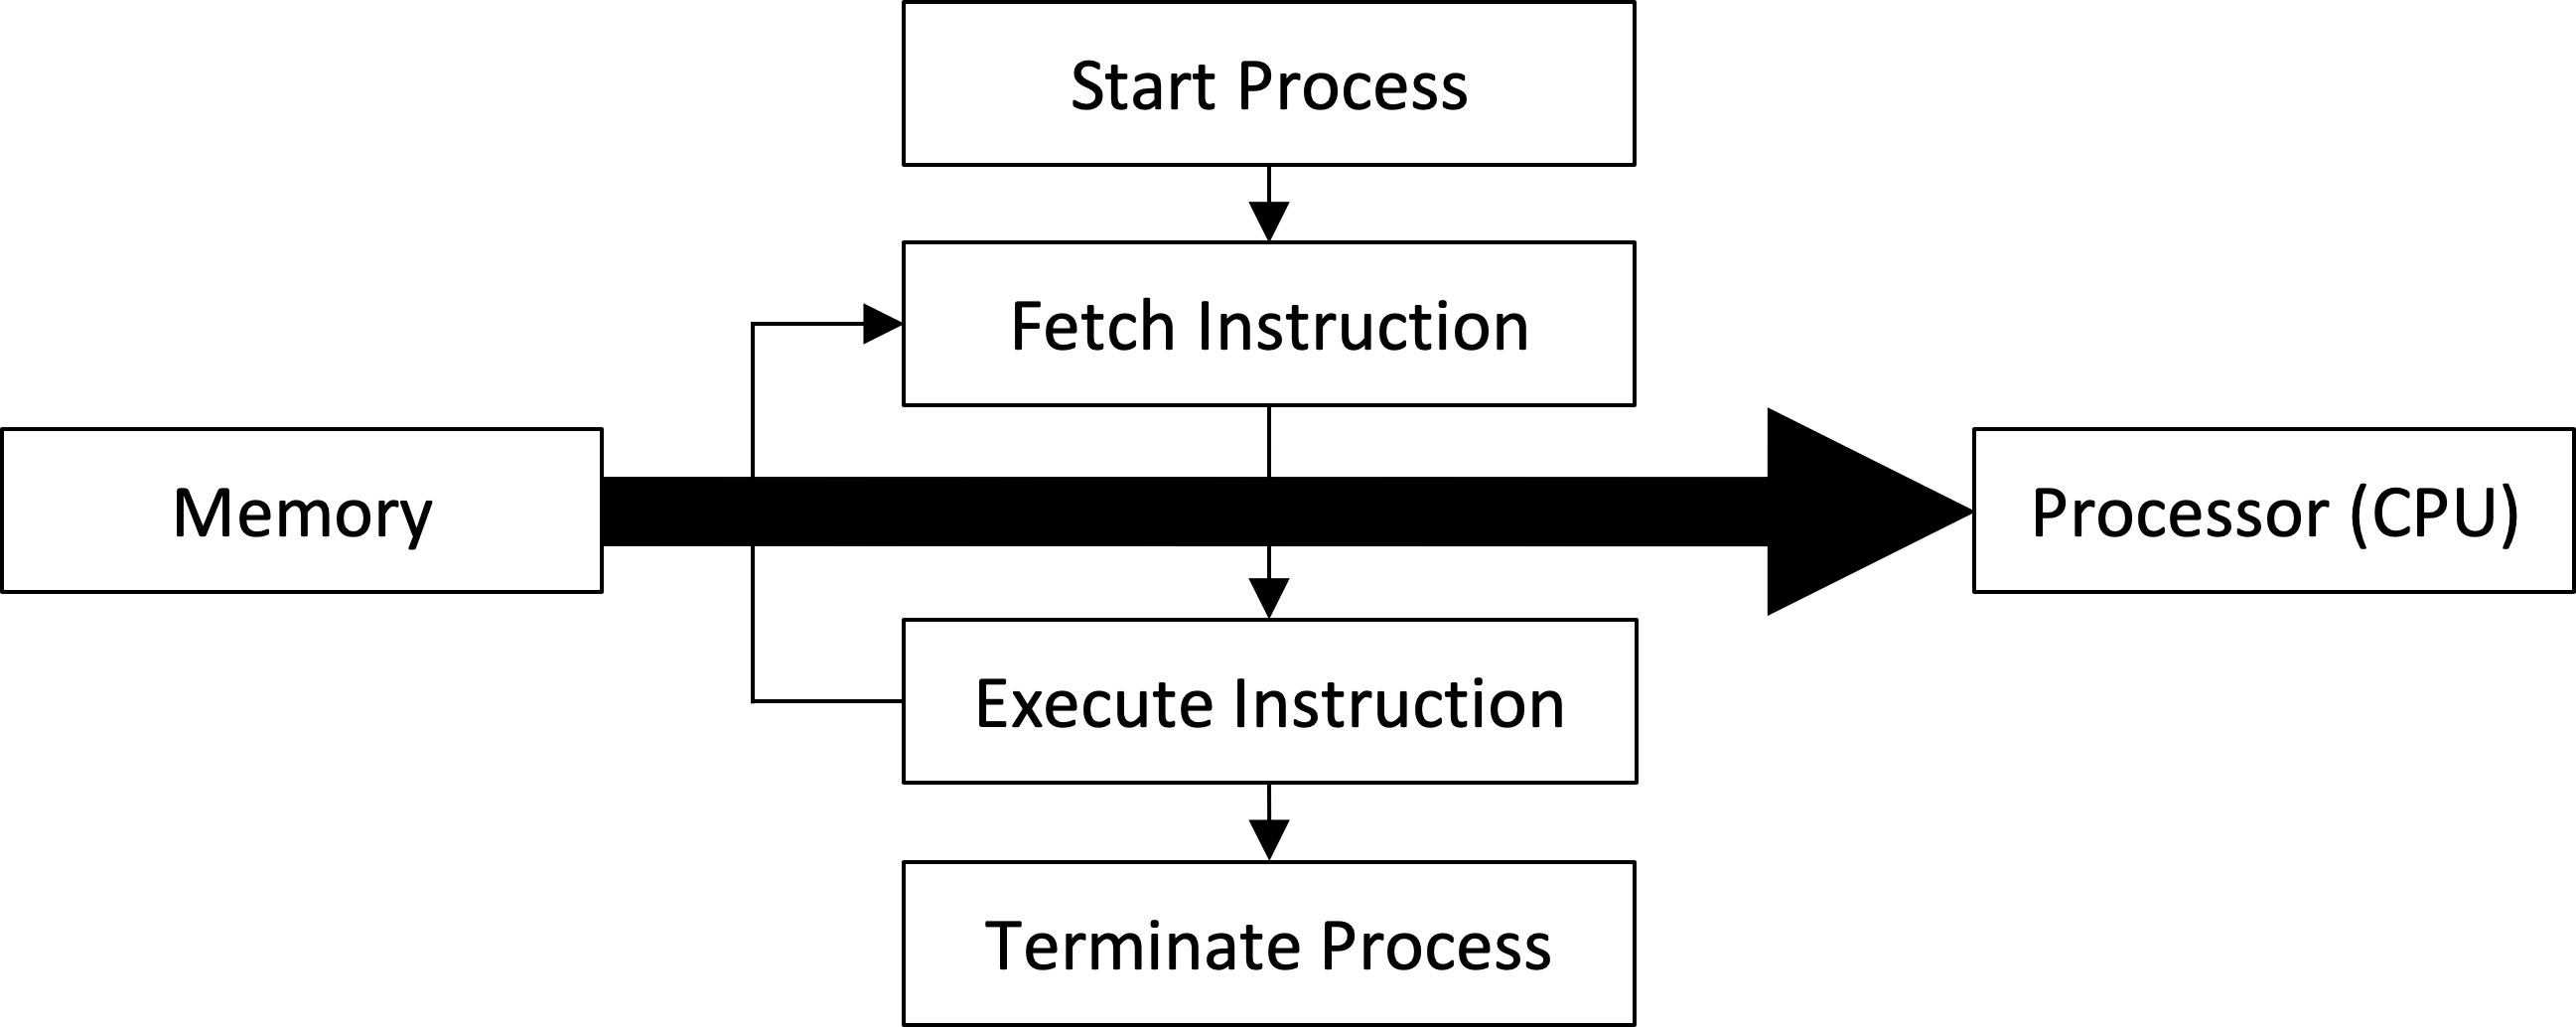
\includegraphics[max size={\textwidth}{\textheight}]{images/chapter-2/simple-fetch-execute-cycle.png}
  \end{minipage}}
  \fbox{\begin{minipage}{\dimexpr \textwidth-2\fboxsep-2\fboxrule}
    \abovecaptionskip=0pt
    \caption{Simple fetch-execute cycle}
  \end{minipage}}
\end{figure}

Once a process is started, instructions are fetched from memory and executed using the CPU. This process will continue until the process is terminated.

This predictable cycle is only feasible to an extent as some processes may be slow or blocked and other may require immediate attention and cannot wait for the current process to terminate. For example, if a process blocks the processor (CPU) because it is waiting for an event to occur, such as a printer to finish its job, or if a high-priority process is supposed to execute as soon as possible. In these cases, interrupts are required.


\section*{Interrupts}

\subsection*{Definition}

An \textbf{interrupt} is a signal sent to the processor indicating that an event caused by hardware or software requires immediate attention.


\subsection*{Types of interrupts}

\begin{longtabu} to \textwidth { X[1.5,l] X[0.2,l] X[7,l]}
	\textbf{\textbullet Input/output (I/O) interrupt}
	& -- &
	Caused by an input/output (I/O) device to signal completion or an error.
	\\
	\\
	\textbf{\textbullet Timer interrupt}
	& -- &
	Caused by a processor timer and is used to alert the operating system (OS) at specific instants.
	\\
	\\
	\textbf{\textbullet Program interrupt}
	& -- &
	Caused by error conditions within user programs or fatal errors.
\end{longtabu}


\subsection*{When do interrupts occur?}

\begin{figure}[H]
  \lineskip=-\fboxrule
  \fbox{\begin{minipage}{\dimexpr \textwidth-2\fboxsep-2\fboxrule}
    \centering
    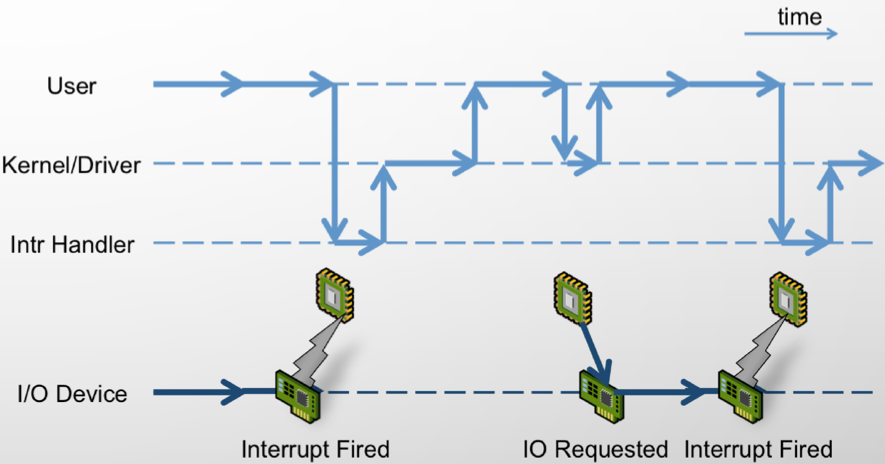
\includegraphics[max size={\textwidth}{\textheight}]{images/chapter-2/interrupt-graph.png}
  \end{minipage}}
  \fbox{\begin{minipage}{\dimexpr \textwidth-2\fboxsep-2\fboxrule}
    \centering
	A process requiring immediate attention is waiting for the processor (CPU).
	
	For example, an input/output (I/O) event occurs.
	
	$\downarrow$
	
	The currently running process’ execution is suspended.
	
	$\downarrow$
	
	Processor switches execution to another process.
	
	$\downarrow$
	
	When input/output (I/O) completes, an interrupt will occur.
	
	$\downarrow$
	
	The execution is diverted to the interrupt handling routine.
	
	An interrupt handling routine (ISR) contains the operations that are performed to deal with an interrupt. Different types of interrupts can have different routines.
	
	$\downarrow$
	
	The suspended program may restart, if conditions are met.
	\end{minipage}}
  \fbox{\begin{minipage}{\dimexpr \textwidth-2\fboxsep-2\fboxrule}
    \abovecaptionskip=0pt
    \caption{Interrupt occurring due to input/output (I/O) event}
  \end{minipage}}
\end{figure}

Interrupts enable operating systems (OSs) to oversee several programs and input/output (I/O) events simultaneously.

This also means that single-core processors can effectively emulate the way in which multi-core processors deal with multiple instructions at a given time by switching between instructions intelligently. Due to the high clock speeds of modern processors, it is easy to give the illusion that true multi-tasking, where two instructions are being processed at once, is taking place on a single-core processor.


\subsection*{Updated fetch-execute cycle}

Given the introduction of interrupts, it is now necessary to update the fetch-execute cycle in order to include the possibility of an interrupt.

\begin{figure}[H]
  \lineskip=-\fboxrule
  \fbox{\begin{minipage}{\dimexpr \textwidth-2\fboxsep-2\fboxrule}
    \centering
    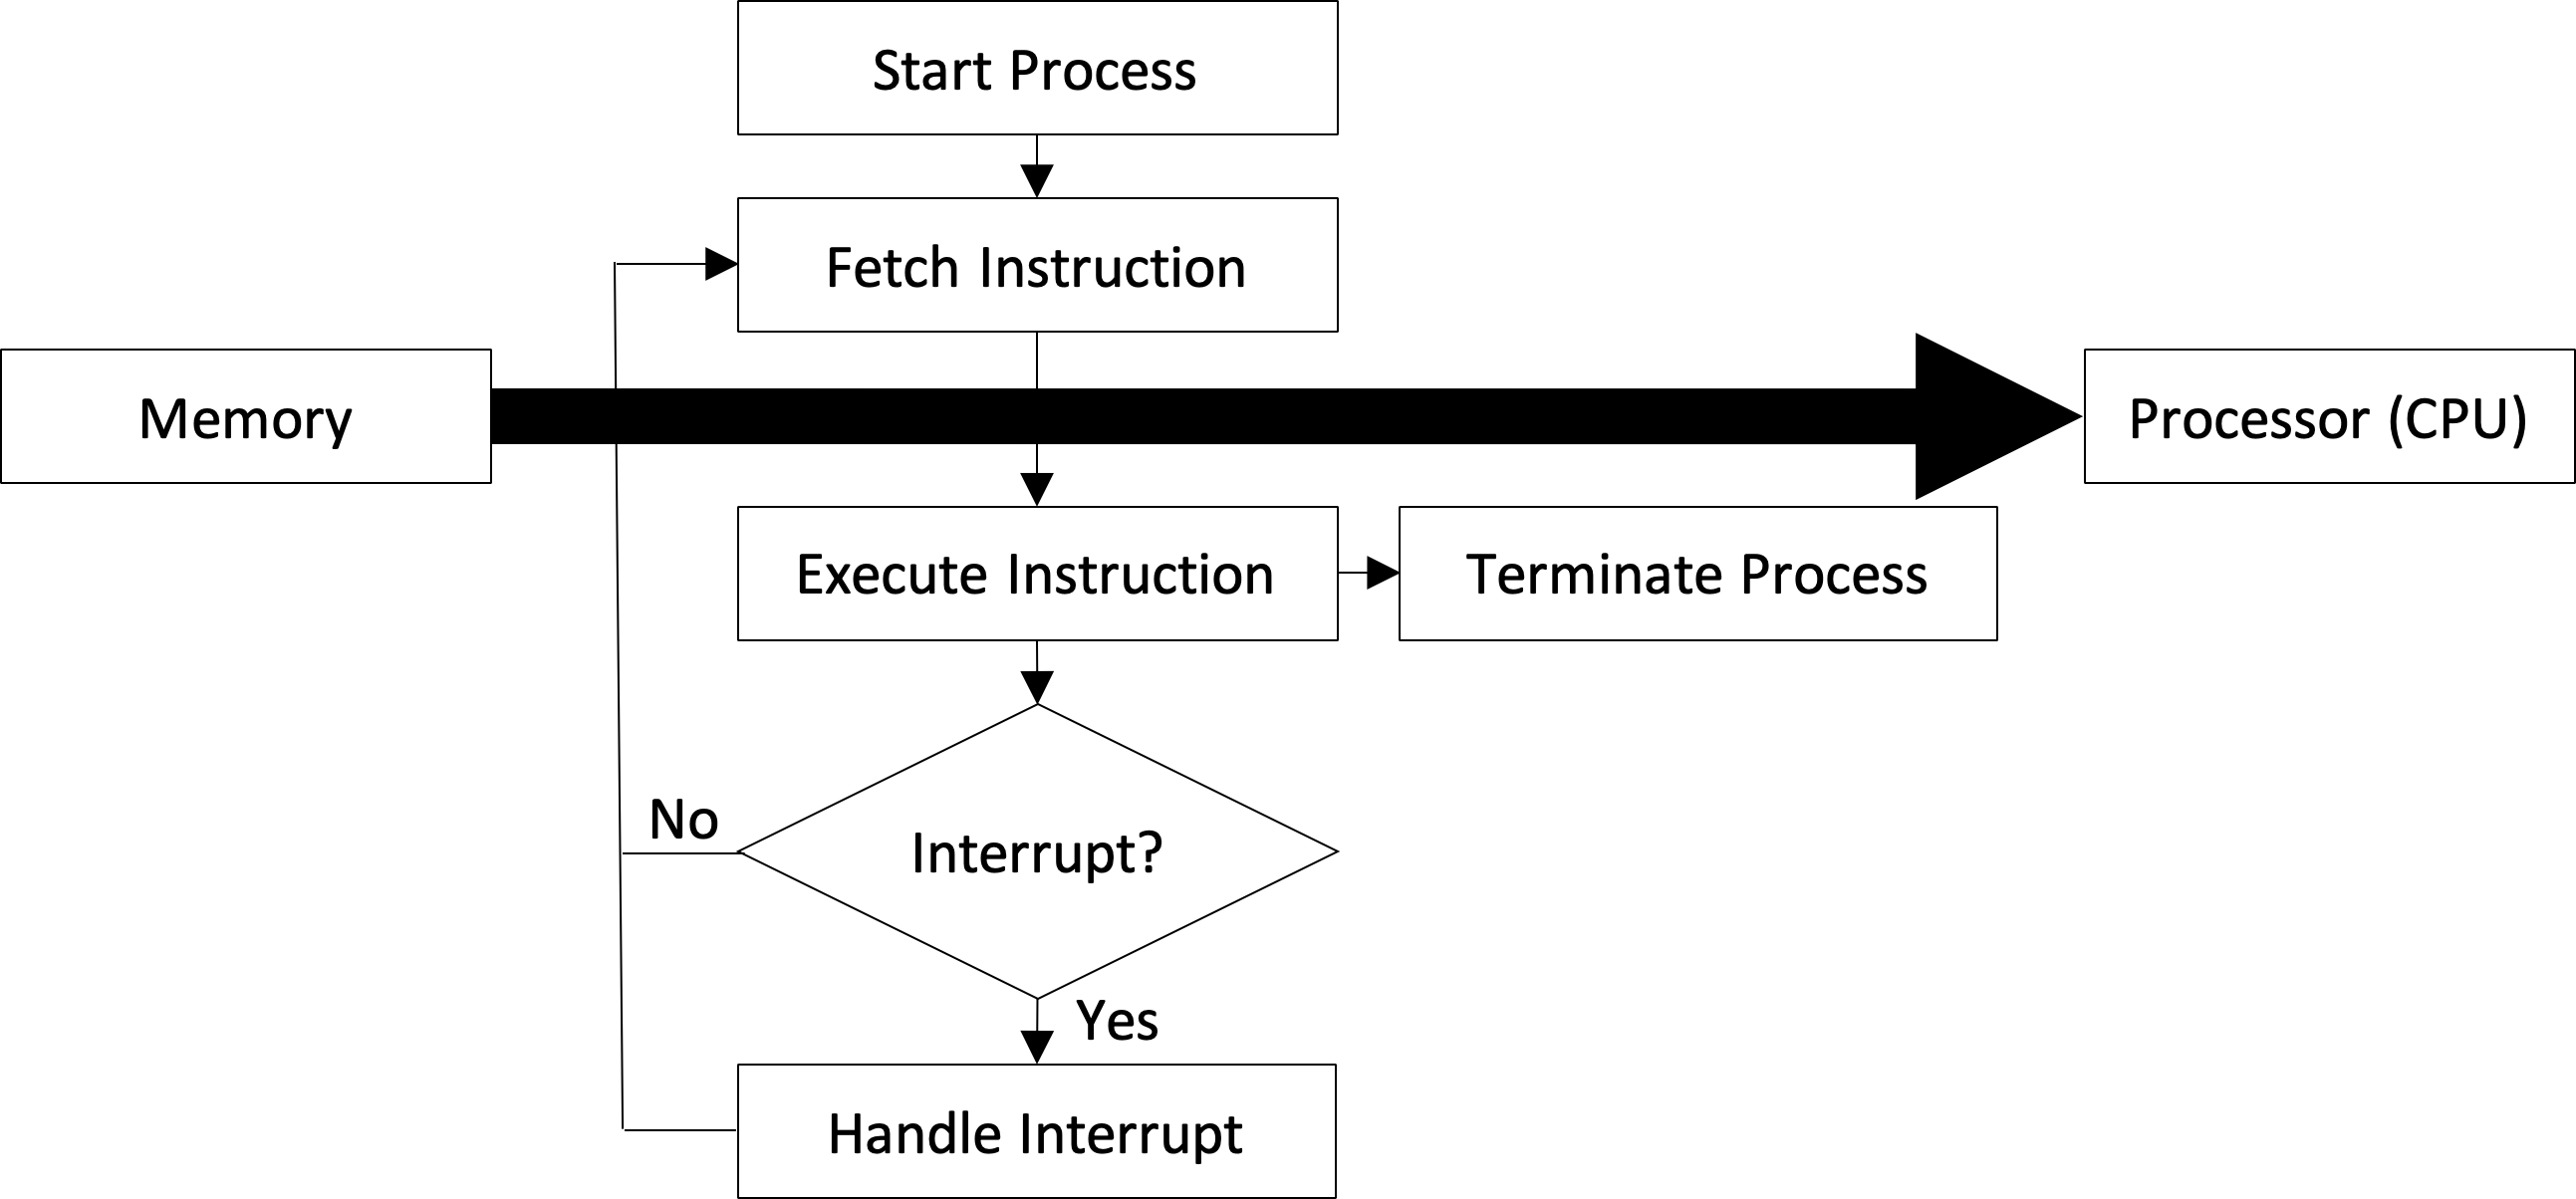
\includegraphics[max size={\textwidth}{\textheight}]{images/chapter-2/updated-fetch-execute-cycle.png}
  \end{minipage}}
  \fbox{\begin{minipage}{\dimexpr \textwidth-2\fboxsep-2\fboxrule}
    \abovecaptionskip=0pt
    \caption{Updated fetch-execute cycle}
  \end{minipage}}
\end{figure}


\section{Concurrency}

\section*{Definition}

\textbf{Concurrency} describes the ability for a program to be decomposed in to parts that can run independently of each other. This means that tasks can be executed out of order and the result would still be the same as if they are executed in order.


\section*{Why is concurrency required}

Concurrency allows the processor (CPU) to run several processes. An example of this is shown by an interrupt occurring due to an input/output (I/O) event occurring (page 24).


\section*{Interleaving}

Concurrency is able to achieve multitasking, that does not require parallel execution, by performing interleaved execution.


\begin{figure}[H]
  \lineskip=-\fboxrule
  \fbox{\begin{minipage}{0.4935\dimexpr \textwidth-2\fboxsep-2\fboxrule}
  	\centering
  	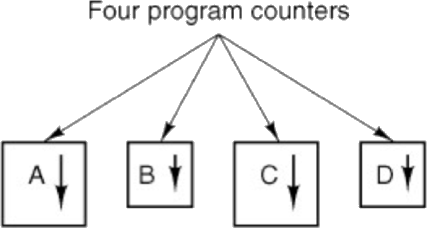
\includegraphics[max size={\textwidth}{\textheight}]{images/chapter-2/interleaving-program-counters.png}
  \end{minipage}
  \begin{minipage}{0.5\dimexpr \textwidth-2\fboxsep-2\fboxrule}
  	\centering
  	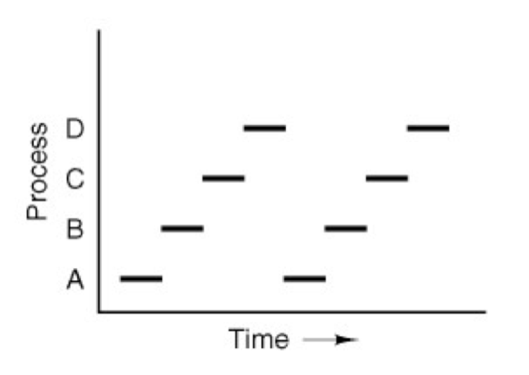
\includegraphics[max size={\textwidth}{\textheight}]{images/chapter-2/interleaving-graph.png}
  \end{minipage}}
  \fbox{\begin{minipage}{\dimexpr \textwidth-2\fboxsep-2\fboxrule}
    \abovecaptionskip=0pt
    \caption{Interleaving}
  \end{minipage}}
\end{figure}


\section{Process scheduling}

\section*{The scheduler}

\subsection*{Definition}

A \textbf{scheduler} uses a scheduling algorithm to determine how to share processor time.


\subsection*{How it works}

After an input/output (I/O) system call or interrupt handling, control is passed to the scheduler to decide which process to execute next.

\begin{figure}[H]
  \lineskip=-\fboxrule
  \fbox{\begin{minipage}{\dimexpr \textwidth-2\fboxsep-2\fboxrule}
    \centering
    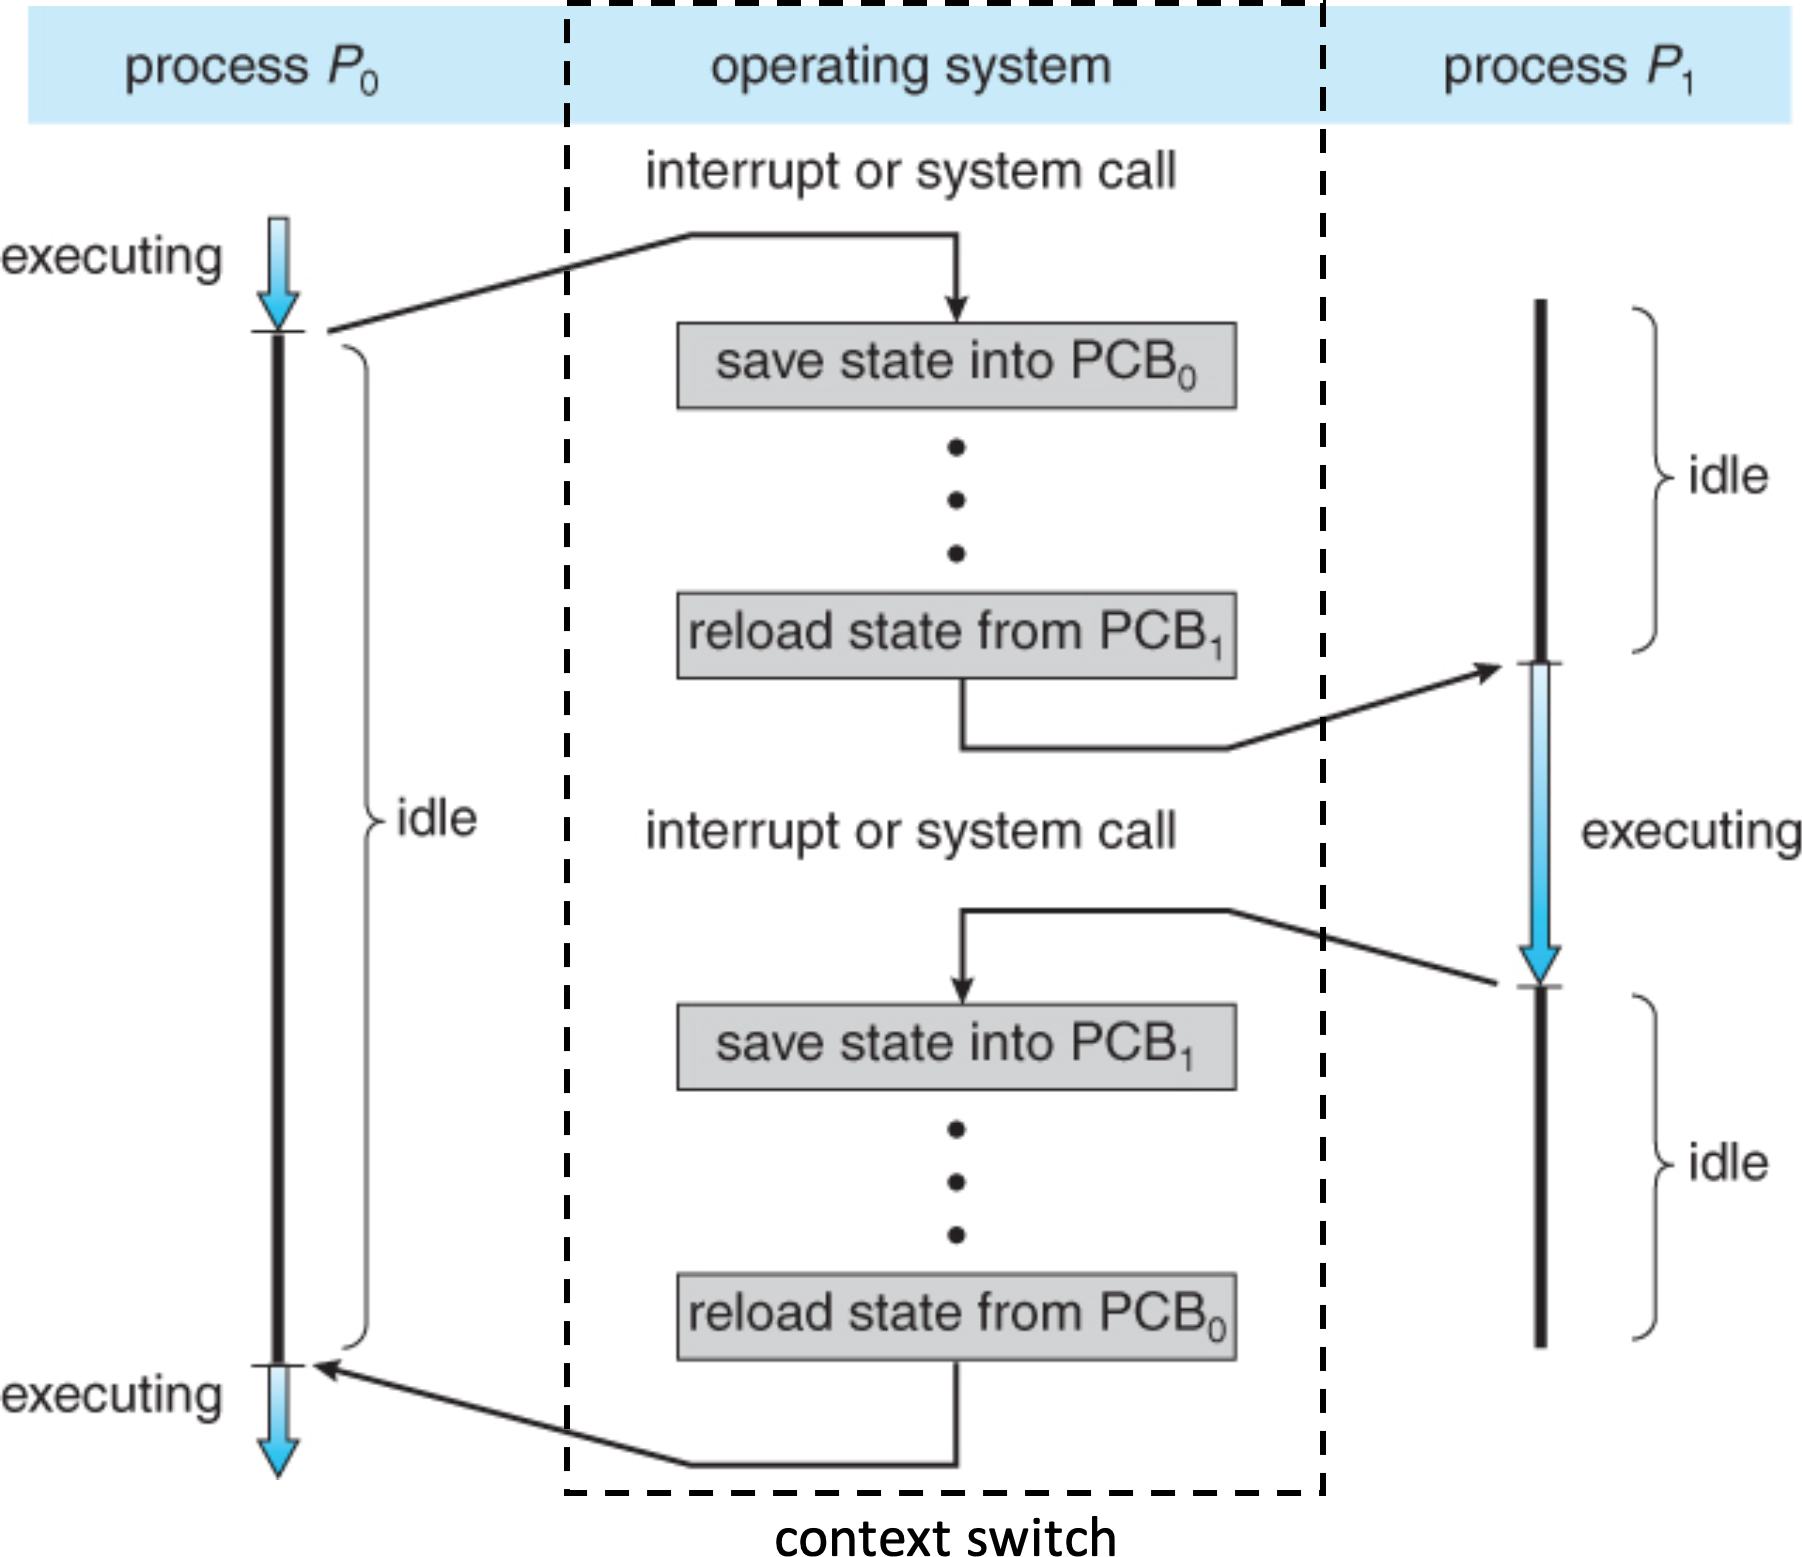
\includegraphics[max size={\textwidth}{\textheight}]{images/chapter-2/the-scheduler.png}
  \end{minipage}}
  \fbox{\begin{minipage}{\dimexpr \textwidth-2\fboxsep-2\fboxrule}
    \abovecaptionskip=0pt
    \caption{The scheduler}
  \end{minipage}}
\end{figure}

The scheduler checks if the current process is still the most suitable to run at this moment in time. If it is control is returned to the process, otherwise:
\begin{itemize}
	\item the state of the current process is saved in the process control block (PCB);
	\item the state of the most suitable process is retrieved from the process control block (PCB); and
	\item control is transferred to the newly selected process at the point indicated by the restored program counter (PC).
\end{itemize}

The action of storing the state of the current process and activating another process is called a context switch.

Context switching must be minimised to reduce overheads created by copying the state of processed and the time taken to perform the switch. However, it is still regarded as important to context switch when appropriate to avoid longer waiting times in the event of a blocked process.


\section*{Scheduling}

\subsection*{Definition}

\textbf{Scheduling} is the act of determining the optimal sequence and timing of assigning execution to processes.


\subsection*{Scheduling criteria}

Different scheduling criteria may be selected depending on the use case for a given computer system.

\begin{longtabu} to \textwidth { X[1.5,l] X[0.2,l] X[7,l]}
	\textbf{\textbullet CPU utilisation}
	& -- &
	Aims to keep the CPU as busy as possible.
	\\
	\\
	\textbf{\textbullet Efficiency}
	& -- &
	Aims to maximise system throughput.
	\\
	\\
	\textbf{\textbullet Fairness}
	& -- &
	Aims to be fair to all running processes or to all users on a multi-user operating system (OS).
\end{longtabu}

This means that different policies and algorithms for scheduling will exist to match these criteria.


\section*{Scheduling policies}

A \textbf{non-preemptive scheduling policy} is one that allows processes to run until complete or incurring an input/output (I/O) wait. These scheduling policies can be described as passive.

A \textbf{preemptive scheduling policy} is one that allows processes to be interrupted and replaced by other processes, generally through timer interrupts.


\section*{Scheduling algorithms}

\subsection*{Definitions}

\textbf{Arrival time} is the instant at which a process is first created.

\textbf{Service time} is the time that it takes for a process to complete if it is in continuous execution.

The \textbf{waiting time} for a process is the sum of time spent in the ready queue during the life of the process. This does not include time that the process is blocked or waiting for input/output (I/O).

In order for a scheduling algorithm to be deemed as fair to all processes, the ratio between waiting time and run time should be about the same for each process.


\subsection*{Case study}

\begin{figure}[H]
  \lineskip=-\fboxrule
  \fbox{\begin{minipage}{\dimexpr \textwidth-2\fboxsep-2\fboxrule}
    \begin{longtabu} to \textwidth {|X[1,c]|X[1,c]|X[1,c]|}
	    \hline
	    \textbf{Process} & \textbf{Arrival Time} & \textbf{Service Time}
	    \\ \hline
	    A & 0 & 3
	    \\ \hline
	    B & 2 & 6
	    \\ \hline
	    C & 4 & 4
	    \\ \hline
	    D & 6 & 5
	    \\ \hline
	    E & 8 & 2
		\\ \hline
	\end{longtabu}
  \end{minipage}}
  \fbox{\begin{minipage}{\dimexpr \textwidth-2\fboxsep-2\fboxrule}
    \abovecaptionskip=0pt
    \caption{Case study}
  \end{minipage}}
\end{figure}

The case study shows different processes (A-E) that all have different arrival times and different service times.

The following examples of scheduling algorithms will refer to this case study to demonstrate their function.


\subsection*{First come, first served (FCFS) / First in, first out (FIFO) – Non-preemptive}

In this algorithm, the first process to arrive is assigned to the processor (CPU) until it is finished. Meanwhile, any other processes that come along are queued up waiting to be processed.

\begin{figure}[H]
  \lineskip=-\fboxrule
  \fbox{\begin{minipage}{0.2935\dimexpr \textwidth-2\fboxsep-2\fboxrule}
  	\centering
  	\begin{longtabu} to \textwidth {|X[1,c]|X[1,c]|X[1,c]|}
	    \hline
	    \textbf{Process} & \textbf{Arrival Time} & \textbf{Service Time}
	    \\ \hline
	    A & 0 & 3
	    \\ \hline
	    B & 2 & 6
	    \\ \hline
	    C & 4 & 4
	    \\ \hline
	    D & 6 & 5
	    \\ \hline
	    E & 8 & 2
		\\ \hline
	\end{longtabu}
  \end{minipage}
  \begin{minipage}{0.7\dimexpr \textwidth-2\fboxsep-2\fboxrule}
  	\centering
  	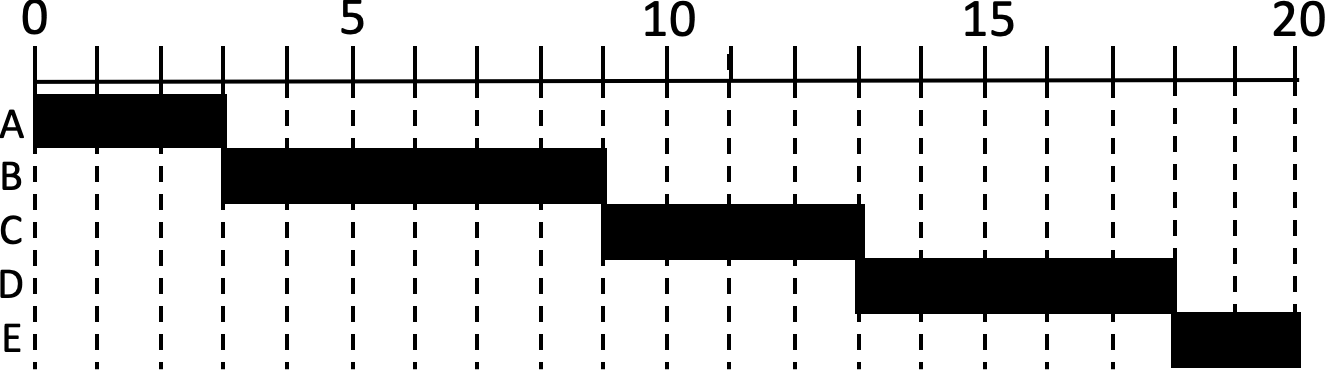
\includegraphics[max size={\textwidth}{\textheight}]{images/chapter-2/temporal-diagram-fcfs.png}
  \end{minipage}}
  \fbox{\begin{minipage}{\dimexpr \textwidth-2\fboxsep-2\fboxrule}
    \abovecaptionskip=0pt
    \caption{Temporal diagram for FCFS / FIFO}
  \end{minipage}}
\end{figure}

\begin{longtabu} to \textwidth {|X[1,l]|X[1,l]|}
    \hline
    \textbf{Advantages} & \textbf{Disadvantages}
    \\ \hline
    \textbf{Simple to implement}.
    &
    \textbf{Does not consider the priority of a process} and therefore the important processes may not be completed quickly.
    \\ \hline
    &
    \textbf{Prevents other processes from starting} while another is in progress and therefore, if processes are of varying sizes, there may be inefficiencies since a single process may take a long time to complete therefore leaving the user waiting before they can perform any other actions.
	\\ \hline
	\multicolumn{2}{|p{\textwidth}|}{\textbf{Favours long processes} as all processes are given the opportunity to run until completion and therefore, some shorter processes may not be able to start processing until the longer processes are finished.}
	\\ \hline
\end{longtabu}
	

\subsection*{Shortest job first (SJF) – Non-preemptive}

In this algorithm, the process with the shortest estimated run time is assigned to the processor (CPU) until it is finished. Meanwhile, any other processes that come along are queued up waiting to be processed.

\begin{figure}[H]
  \lineskip=-\fboxrule
  \fbox{\begin{minipage}{0.2935\dimexpr \textwidth-2\fboxsep-2\fboxrule}
  	\centering
  	\begin{longtabu} to \textwidth {|X[1,c]|X[1,c]|X[1,c]|}
	    \hline
	    \textbf{Process} & \textbf{Arrival Time} & \textbf{Service Time}
	    \\ \hline
	    A & 0 & 3
	    \\ \hline
	    B & 2 & 6
	    \\ \hline
	    C & 4 & 4
	    \\ \hline
	    D & 6 & 5
	    \\ \hline
	    E & 8 & 2
		\\ \hline
	\end{longtabu}
  \end{minipage}
  \begin{minipage}{0.7\dimexpr \textwidth-2\fboxsep-2\fboxrule}
  	\centering
  	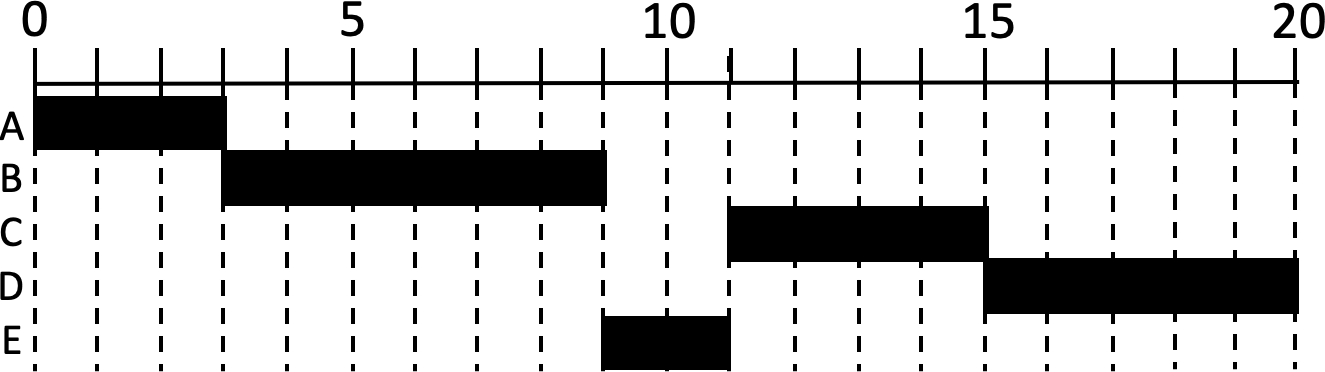
\includegraphics[max size={\textwidth}{\textheight}]{images/chapter-2/temporal-diagram-sjf.png}
  \end{minipage}}
  \fbox{\begin{minipage}{\dimexpr \textwidth-2\fboxsep-2\fboxrule}
    \abovecaptionskip=0pt
    \caption{Temporal diagram for SJF}
  \end{minipage}}
\end{figure}

\begin{longtabu} to \textwidth {|X[1,l]|X[1,l]|}
    \hline
    \textbf{Advantages} & \textbf{Disadvantages}
    \\ \hline
    \textbf{Simple to implement}.
    &
    \textbf{Does not consider the priority of a process} and therefore the important processes may not be completed quickly.
    \\ \hline
  	\textbf{Shorter processes are processed quickly} because they take precedence.
    &
    \textbf{Relies on an estimation} of how long a process will take which could be incorrect.
    \\ \hline
  	\textbf{Minimises the average time taken to complete a process} because the shortest processes take precedence.
    &
    \textbf{Prevents other processes from starting} while another is in progress and therefore, if processes are of varying sizes, there may be inefficiencies since a single process may take a long time to complete therefore leaving the user waiting before they can perform any other actions.
	\\ \hline
	\multicolumn{2}{|p{\textwidth}|}{\textbf{Favours long processes} as the processes with the shortest estimated time are given the opportunity to run until completion and therefore, some longer processes may not be able to start processing until there are no more shorter processes currently running or ready to be processed.}
	\\ \hline
\end{longtabu}


\subsection*{Shortest remaining time (SRT) – Preemptive}

In this algorithm, the process with the shortest estimated remaining time is assigned to the processor (CPU). If a process becomes ready that has a shorter remaining time, it will be pre-empted to allow the new process to start and the scheduler is switched to that new process.

\begin{figure}[H]
  \lineskip=-\fboxrule
  \fbox{\begin{minipage}{0.2935\dimexpr \textwidth-2\fboxsep-2\fboxrule}
  	\centering
  	\begin{longtabu} to \textwidth {|X[1,c]|X[1,c]|X[1,c]|}
	    \hline
	    \textbf{Process} & \textbf{Arrival Time} & \textbf{Service Time}
	    \\ \hline
	    A & 0 & 3
	    \\ \hline
	    B & 2 & 6
	    \\ \hline
	    C & 4 & 4
	    \\ \hline
	    D & 6 & 5
	    \\ \hline
	    E & 8 & 2
		\\ \hline
	\end{longtabu}
  \end{minipage}
  \begin{minipage}{0.7\dimexpr \textwidth-2\fboxsep-2\fboxrule}
  	\centering
  	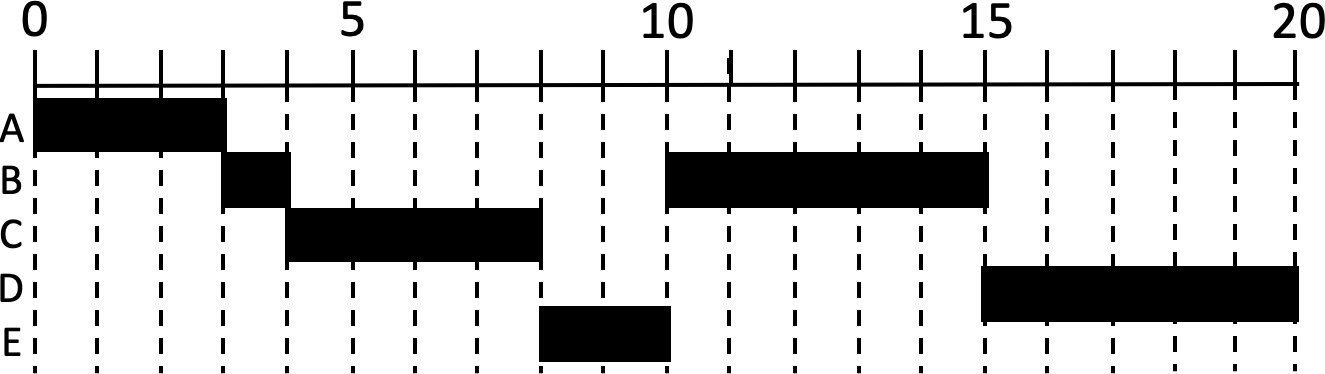
\includegraphics[max size={\textwidth}{\textheight}]{images/chapter-2/temporal-diagram-srt.png}
  \end{minipage}}
  \fbox{\begin{minipage}{\dimexpr \textwidth-2\fboxsep-2\fboxrule}
    \abovecaptionskip=0pt
    \caption{Temporal diagram for SRT}
  \end{minipage}}
\end{figure}

\begin{longtabu} to \textwidth {|X[1,l]|X[1,l]|}
    \hline
    \textbf{Advantages} & \textbf{Disadvantages}
    \\ \hline
    \textbf{High throughput} because the number of processes completed is high due to the shortest processes taking precedence.
    &
    \textbf{Does not consider the priority of a process} and therefore the important processes may not be completed quickly.
    \\ \hline
  	\textbf{Shorter processes are processed quickly} because they take precedence.
    &
    \textbf{Relies on an estimation} of how long a process will take which could be incorrect.
    \\ \hline
  	
    &
    \textbf{Can be inefficient} if a large process is in progress and shorter processes are being added to the queue because they will take precedence.
	\\ \hline
	\multicolumn{2}{|p{\textwidth}|}{\textbf{Favours long processes} as the processes with the shortest estimated time are given the opportunity to run until a process with a shorter estimated time is ready and therefore, some longer processes may not be able to start processing until there are no more shorter processes currently running or ready to be processed.}
	\\ \hline
\end{longtabu}


\subsection*{Highest response ratio next (HRRN) – Preemptive}

In this algorithm, the process with the highest priority is assigned to the processor (CPU). If a process becomes ready that has a higher priority, it will be pre-empted to allow the new process to start and the scheduler is switched to that new process.

The priority of a process may be based on memory, time and/or any other resource requirement such as:
\[\frac{waiting time + run time}{run time}\]

\begin{figure}[H]
  \lineskip=-\fboxrule
  \fbox{\begin{minipage}{0.2935\dimexpr \textwidth-2\fboxsep-2\fboxrule}
  	\centering
  	\begin{longtabu} to \textwidth {|X[1,c]|X[1,c]|X[1,c]|}
	    \hline
	    \textbf{Process} & \textbf{Arrival Time} & \textbf{Service Time}
	    \\ \hline
	    A & 0 & 3
	    \\ \hline
	    B & 2 & 6
	    \\ \hline
	    C & 4 & 4
	    \\ \hline
	    D & 6 & 5
	    \\ \hline
	    E & 8 & 2
		\\ \hline
	\end{longtabu}
  \end{minipage}
  \begin{minipage}{0.7\dimexpr \textwidth-2\fboxsep-2\fboxrule}
  	\centering
  	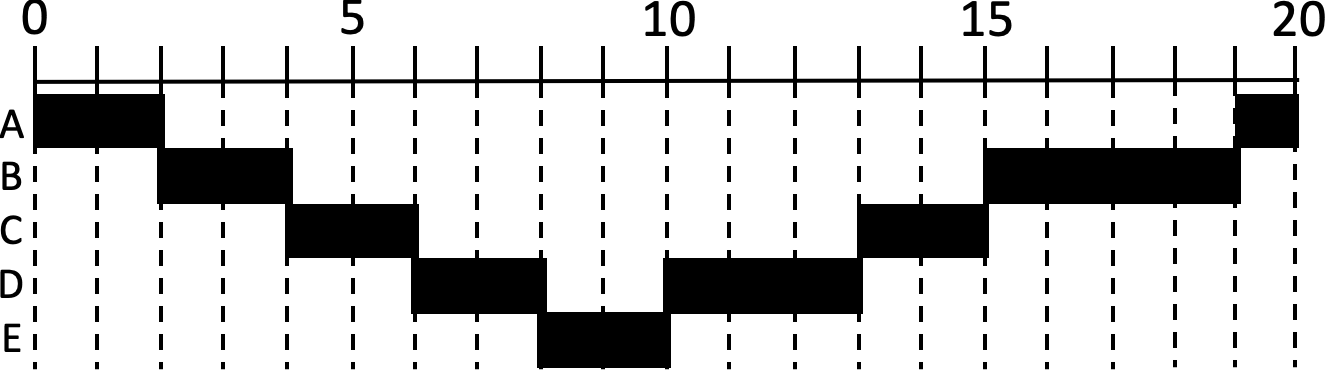
\includegraphics[max size={\textwidth}{\textheight}]{images/chapter-2/temporal-diagram-hrrn.png}
  	This diagram assumes that the processes are assigned a letter in reverse order of priority, such that E has the greatest priority and A has the lowest priority.
  \end{minipage}}
  \fbox{\begin{minipage}{\dimexpr \textwidth-2\fboxsep-2\fboxrule}
    \abovecaptionskip=0pt
    \caption{Temporal diagram for HRRN}
  \end{minipage}}
\end{figure}

\begin{longtabu} to \textwidth {|X[1,l]|X[1,l]|}
    \hline
    \textbf{Advantages} & \textbf{Disadvantages}
    \\ \hline
    \textbf{High throughput} because the number of processes completed is high due to the shortest processes taking precedence.
    &
    \textbf{Does not consider the priority of a process} and therefore the important processes may not be completed quickly.
    \\ \hline
  	\textbf{Shorter processes are processed quickly} because they take precedence.
    &
    \textbf{Relies on an estimation} of how long a process will take which could be incorrect.
    \\ \hline
  	
    &
    \textbf{Can be inefficient} if a large process is in progress and shorter processes are being added to the queue because they will take precedence.
	\\ \hline
\end{longtabu}


\subsection*{Round robin (RR) – Preemptive}

In this algorithm, each process is dispatched to the processor (CPU) on a “first in, first out” (FIFO) basis with a fixed time quantum.

Each time quantum is typically 10-20ms. Modern processor (CPU) clock frequencies are typically greater than 2GHz, which implies clock periods of 5×10$^{-7}$ms. This shows that the given time quantum is relatively large compared to a typically processor’s (CPU’s) clock period.

If a process experiences a timeout, this will mean that it has run over its fixed time quantum. In which case, the process will be interrupted and returned to the back of the queue.

A system designer may wish to choose a time quantum that is most appropriate for a given system. This may be done by measuring the average service time and waiting time for the processes that will be running on the system and design the fixed time quantum around these figures. It may be that a system designer wishes to minimise the number of processes that are interrupted by another process.

\begin{figure}[H]
  \lineskip=-\fboxrule
  \fbox{\begin{minipage}{\dimexpr \textwidth-2\fboxsep-2\fboxrule}
    \centering
    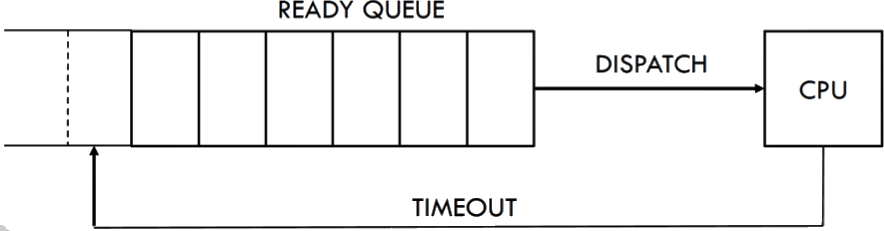
\includegraphics[max size={\textwidth}{\textheight}]{images/chapter-2/round-robin.png}
  \end{minipage}}
  \fbox{\begin{minipage}{\dimexpr \textwidth-2\fboxsep-2\fboxrule}
    \abovecaptionskip=0pt
    \caption{RR}
  \end{minipage}}
\end{figure}

\begin{figure}[H]
  \lineskip=-\fboxrule
  \fbox{\begin{minipage}{0.2935\dimexpr \textwidth-2\fboxsep-2\fboxrule}
  	\centering
  	\begin{longtabu} to \textwidth {|X[1,c]|X[1,c]|X[1,c]|}
	    \hline
	    \textbf{Process} & \textbf{Arrival Time} & \textbf{Service Time}
	    \\ \hline
	    A & 0 & 3
	    \\ \hline
	    B & 2 & 6
	    \\ \hline
	    C & 4 & 4
	    \\ \hline
	    D & 6 & 5
	    \\ \hline
	    E & 8 & 2
		\\ \hline
	\end{longtabu}
  \end{minipage}
  \begin{minipage}{0.7\dimexpr \textwidth-2\fboxsep-2\fboxrule}
  	\centering
  	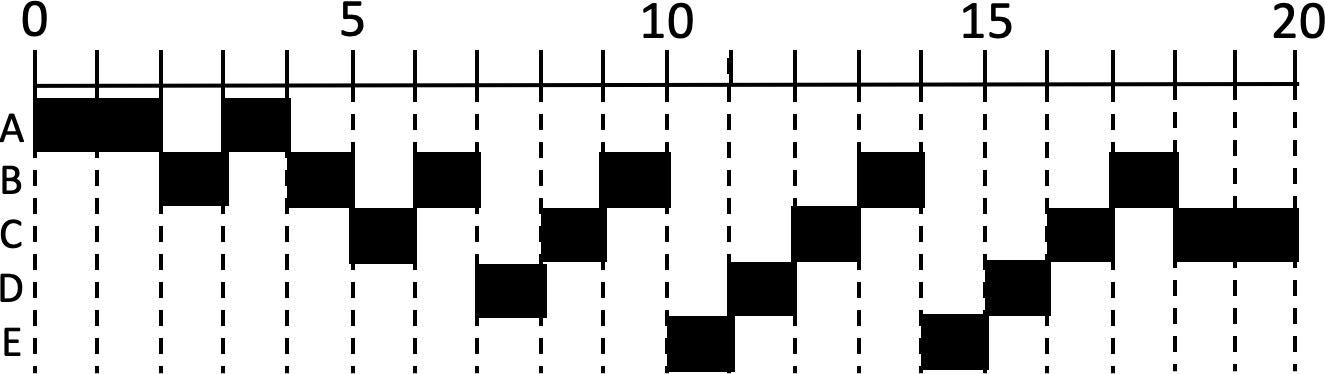
\includegraphics[max size={\textwidth}{\textheight}]{images/chapter-2/temporal-diagram-rr-1.png}
  \end{minipage}}
  \fbox{\begin{minipage}{\dimexpr \textwidth-2\fboxsep-2\fboxrule}
    \abovecaptionskip=0pt
    \caption{Temporal diagram for RR with a fixed time quantum of 1 (q = 1)}
  \end{minipage}}
\end{figure}

\begin{figure}[H]
  \lineskip=-\fboxrule
  \fbox{\begin{minipage}{0.2935\dimexpr \textwidth-2\fboxsep-2\fboxrule}
  	\centering
  	\begin{longtabu} to \textwidth {|X[1,c]|X[1,c]|X[1,c]|}
	    \hline
	    \textbf{Process} & \textbf{Arrival Time} & \textbf{Service Time}
	    \\ \hline
	    A & 0 & 3
	    \\ \hline
	    B & 2 & 6
	    \\ \hline
	    C & 4 & 4
	    \\ \hline
	    D & 6 & 5
	    \\ \hline
	    E & 8 & 2
		\\ \hline
	\end{longtabu}
  \end{minipage}
  \begin{minipage}{0.7\dimexpr \textwidth-2\fboxsep-2\fboxrule}
  	\centering
  	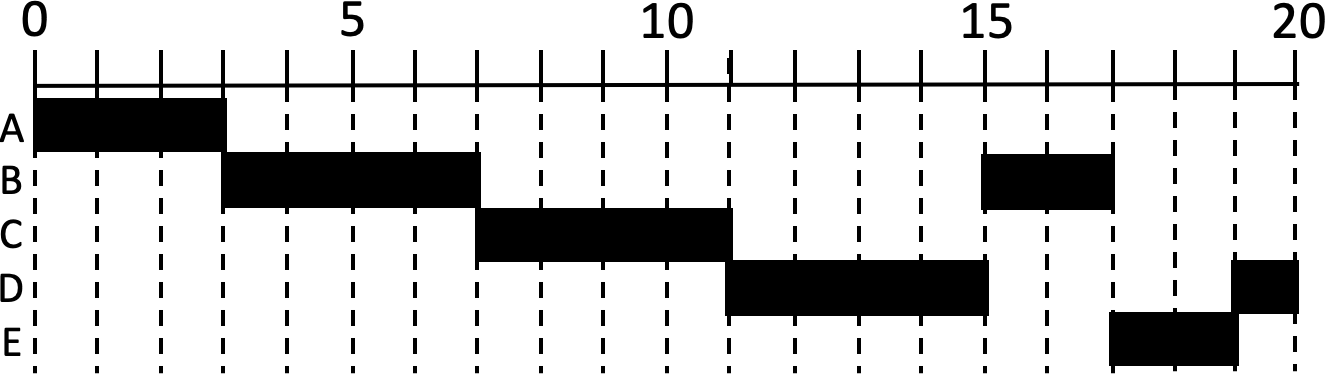
\includegraphics[max size={\textwidth}{\textheight}]{images/chapter-2/temporal-diagram-rr-4.png}
  \end{minipage}}
  \fbox{\begin{minipage}{\dimexpr \textwidth-2\fboxsep-2\fboxrule}
    \abovecaptionskip=0pt
    \caption{Temporal diagram for RR with a fixed time quantum of 4 (q = 4)}
  \end{minipage}}
\end{figure}

\begin{longtabu} to \textwidth {|X[1,l]|X[1,l]|}
    \hline
    \textbf{Advantages} & \textbf{Disadvantages}
    \\ \hline
    \textbf{Simple to implement}.
    &
    \textbf{Heavy overhead} due to continuous context switches.
    \\ \hline
  	\textbf{Suitable for some types of computer systems}, such as those which will be running processes of similar priority and size.
    &
    \textbf{Does not consider the priority of a process} and therefore the important processes may not be completed quickly.
    \\ \hline
    &
    \textbf{Does not consider the size of a process} and therefore, if processes are of varying sizes, there may be inefficiencies since a single process may take a long time to complete thus leaving the user waiting before they can perform any other actions.
	\\ \hline
\end{longtabu}


\section*{Multi-level queueing}

\subsection*{Definition}

\textbf{Multi-level queueing} is a queue with a predefined number of levels which consist of several independent queues.


\subsection*{How it works}

Multi-level queueing makes use of other existing scheduling algorithms.

\begin{figure}[H]
  \lineskip=-\fboxrule
  \fbox{\begin{minipage}{\dimexpr \textwidth-2\fboxsep-2\fboxrule}
    \centering
    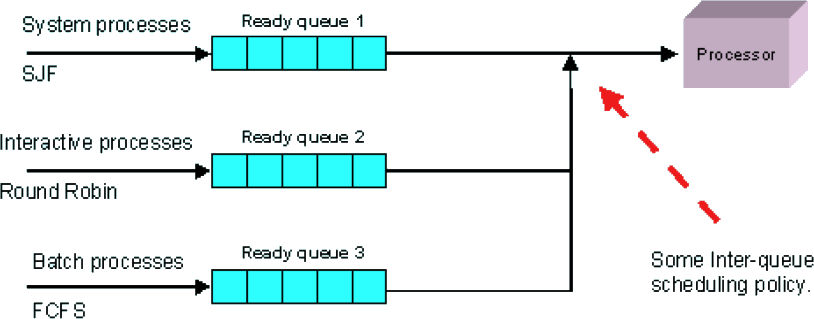
\includegraphics[max size={\textwidth}{\textheight}]{images/chapter-2/multi-level-queueing.png}
  \end{minipage}}
  \fbox{\begin{minipage}{\dimexpr \textwidth-2\fboxsep-2\fboxrule}
    \abovecaptionskip=0pt
    \caption{Multi-level queueing}
  \end{minipage}}
\end{figure}

Each queue has a different priority; the top queue has the highest priority and the bottom queue has the lowest priority. Processes are able to move between queues if their priority changes.

There is some form of inter-queue scheduling policy that governs the assignment of processes from each queue to the processor (CPU).

The queues in a multi-level queueing system may differ between operating system (OS). For example, the scheduler used by the Minix operating system (OS) uses multi-level queueing and implements 16 queues.

\begin{longtabu} to \textwidth {|X[1,l]|X[1,l]|}
    \hline
    \textbf{Advantages} & \textbf{Disadvantages}
    \\ \hline
    \textbf{Allows scheduling optimisation} as a system designer may be able to leverage the advantages of a range of different scheduling algorithms.
    &
    \\ \hline
  	\textbf{Maintains common processes} as it is possible to split processes in to different queues depending on their nature. For example, input/output processes could be in one queue while processor (CPU) processes are in another queue.
    &
    \\ \hline
    \textbf{Helps to prevent bottlenecks} because input/output (I/O) devices are slower than the processor speed and therefore maximising processes involving input/output (I/O) devices ensures that these devices are continuously busy.
    &
	\\ \hline
\end{longtabu}


\chapter{Threads and Concurrency}
\label{chap:3}

\section{What are threads?}

\section*{Definition}

A \textbf{thread} is an independent path/sequence of execution with in a process and can be managed independently by a scheduler. A process many contain many threads.


\section*{Multi-threading}

\subsection*{How it works}

As mentioned in the previous section, a process (or job/task) shows a program in execution and is a particular instance of a program. By default, these processes are run by means of “single execution thread”.

However, different parts of the same process could be parallelised in order to allow multi-threading.

Multi-threading provides a way of improving application performance and therefore improving the efficiency and/or usability of a computer system.

\begin{figure}[H]
  \lineskip=-\fboxrule
  \fbox{\begin{minipage}{\dimexpr \textwidth-2\fboxsep-2\fboxrule}
    \centering
    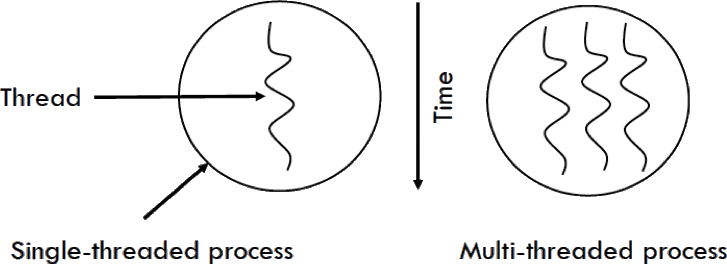
\includegraphics[max size={\textwidth}{\textheight}]{images/chapter-3/single-threaded-vs-multi-threaded.png}
  \end{minipage}}
  \fbox{\begin{minipage}{\dimexpr \textwidth-2\fboxsep-2\fboxrule}
    \abovecaptionskip=0pt
    \caption{Single-threaded vs multi-threaded}
  \end{minipage}}
\end{figure}


\subsection*{Example}

\begin{figure}[H]
  \lineskip=-\fboxrule
  \fbox{\begin{minipage}{0.4935\dimexpr \textwidth-2\fboxsep-2\fboxrule}
  	\centering
  	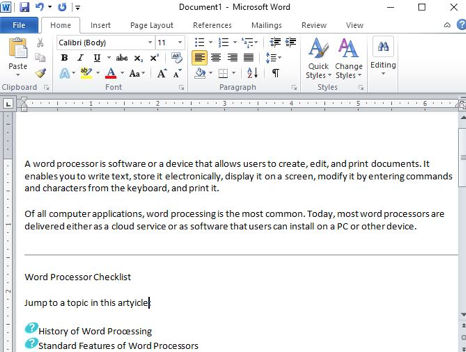
\includegraphics[max size={\textwidth}{\textheight}]{images/chapter-3/microsoft-word.png}
  \end{minipage}
  \begin{minipage}{0.5\dimexpr \textwidth-2\fboxsep-2\fboxrule}
	In this example, a thread could be assigned to each of the following tasks:
	\begin{itemize}
		\item user input, such as keyboard and mouse input;
		\item auto-saving document;
		\item spell-checking document; and
		\item printing in the background.
	\end{itemize}
	This is possible as all of these tasks can be run in parallel as they do not require information from one another.
  \end{minipage}}
  \fbox{\begin{minipage}{\dimexpr \textwidth-2\fboxsep-2\fboxrule}
    \abovecaptionskip=0pt
    \caption{Example of multi-threading in Microsoft Word}
  \end{minipage}}
\end{figure}


\section*{Threads vs processes}

\subsection*{Comparison}

Threads and processes share some similarities however, there are also some distinct differences.

\begin{figure}[H]
  \lineskip=-\fboxrule
  \fbox{\begin{minipage}{\dimexpr \textwidth-2\fboxsep-2\fboxrule}
    \centering
    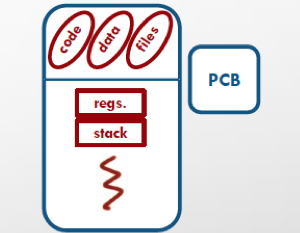
\includegraphics[max size={\textwidth}{\textheight}]{images/chapter-3/single-threaded-process.png}
  \end{minipage}}
  \fbox{\begin{minipage}{\dimexpr \textwidth-2\fboxsep-2\fboxrule}
    \abovecaptionskip=0pt
    \caption{Single-threaded process}
  \end{minipage}}
\end{figure}

\begin{figure}[H]
  \lineskip=-\fboxrule
  \fbox{\begin{minipage}{\dimexpr \textwidth-2\fboxsep-2\fboxrule}
    \centering
    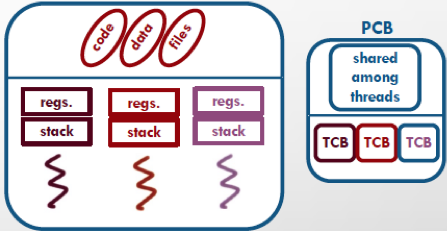
\includegraphics[max size={\textwidth}{\textheight}]{images/chapter-3/multi-threaded-process.png}
  \end{minipage}}
  \fbox{\begin{minipage}{\dimexpr \textwidth-2\fboxsep-2\fboxrule}
    \abovecaptionskip=0pt
    \caption{Multi-threaded process}
  \end{minipage}}
\end{figure}

\begin{figure}[H]
  \lineskip=-\fboxrule
  \fbox{\begin{minipage}{\dimexpr \textwidth-2\fboxsep-2\fboxrule}
    \centering
    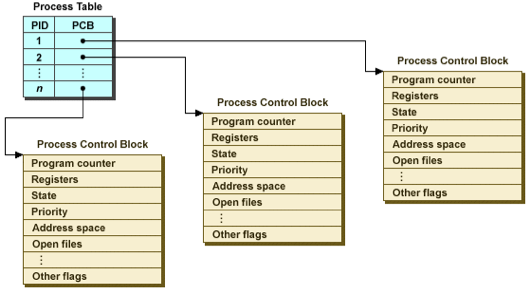
\includegraphics[max size={\textwidth}{\textheight}]{images/chapter-3/process-table-and-control-block.png}
  \end{minipage}}
  \fbox{\begin{minipage}{\dimexpr \textwidth-2\fboxsep-2\fboxrule}
    \abovecaptionskip=0pt
    \caption{Process table and process control blocks}
  \end{minipage}}
\end{figure}

\begin{figure}[H]
  \lineskip=-\fboxrule
  \fbox{\begin{minipage}{\dimexpr \textwidth-2\fboxsep-2\fboxrule}
    \begin{longtabu} to \textwidth {|X[0.8,c]|X[2,l]|X[2,l]|}
	    \hline
	     & \textbf{Threads} & \textbf{Processes}
	    \\ \hline
		\multirow{7}{*}{Similarities}
		& Sequential flow of control with start and end.
		& Sequential flow of control with start and end.
		\\
		\cline{2-3} 
		& At any time, a thread has a single point of execution.
		& At any time, a process has a single point of execution.
		\\
		\cline{2-3} 
		& Has its own execution context, stack (history) and program counter stored in a thread control block (TCB).
		& Has its own execution context, stack (history) and program counter stored in a process control block (PCB).
		\\
		\cline{2-3} 
		& Follows the three-state model in which the thread can be running, blocked or ready.
		& Follows the three-state model in which the process can be running, blocked or ready.
		\\
		\cline{2-3} 
		& Context switching can happen for threads.
		& Context switching can happen for processes.
		\\
		\cline{2-3} 
		& A thread can spawn another thread.
		& A process can spawn another process.
		\\
		\cline{2-3} 
		& A thread is often called a lightweight process. &
		\\ \hline
		\multirow{5}{*}{Differences}
		& A thread cannot exist on its own, instead it exists within a process.
		& A process does not require a parent entity.
		\\
		\cline{2-3} 
		& Usually created and/or controlled by a process.
		& A process is not typically created and/or controlled by another process.
		\\
		\cline{2-3} 
		& Threads can share process properties, including memory and open files.
		& Processes cannot share process properties with other processes.
		\\
		\cline{2-3} 
		& Inexpensive creation and context switching as does not require separate address space.
		& Expensive creation and context switching as requires separate address space.
		\\
		\cline{2-3} 
		& When running multiple threads concurrently, they share an address space.
		& When running multiple processes concurrently, they are resources, such as memory, disk and printers.
		\\ \hline
	\end{longtabu}
  \end{minipage}}
  \fbox{\begin{minipage}{\dimexpr \textwidth-2\fboxsep-2\fboxrule}
    \abovecaptionskip=0pt
    \caption{Threads vs processes}
  \end{minipage}}
\end{figure}


\subsection*{Properties}

\begin{figure}[H]
  \lineskip=-\fboxrule
  \fbox{\begin{minipage}{\dimexpr \textwidth-2\fboxsep-2\fboxrule}
    \begin{longtabu} to \textwidth {|X[1,l]|X[1,l]|}
	    \hline
		\textbf{Per process items}
		& \textbf{Per thread items}
		\\ \hline
		Address space & Program counter
		\\ \hline
		Global variables & Registers
		\\ \hline
		Open files & Stack
		\\ \hline
		Child processes & State
		\\ \hline
		Pending alarms &
		\\ \hline
		Signals and signal handlers &
		\\ \hline
		Accounting information &
		\\ \hline
	\end{longtabu}
  \end{minipage}}
  \fbox{\begin{minipage}{\dimexpr \textwidth-2\fboxsep-2\fboxrule}
    \abovecaptionskip=0pt
    \caption{Threads vs processes}
  \end{minipage}}
\end{figure}

Process properties are shared between threads.
Thread properties are local and private to each thread.


\section{Sequential and concurrent programming}

\section*{Sequential programming}

\subsection*{Definition}

\textbf{Sequential programming} is the traditional activity of constructing a computer program using a sequential programming language.


\subsection*{How it works}

This involves a programming methodology that assumes statements are executed in order/sequence.

Programs written using sequential programming are assumed to execute on a single-CPU system and have a single thread of control.

\begin{figure}[H]
  \lineskip=-\fboxrule
  \fbox{\begin{minipage}{\dimexpr \textwidth-2\fboxsep-2\fboxrule}
    \centering
    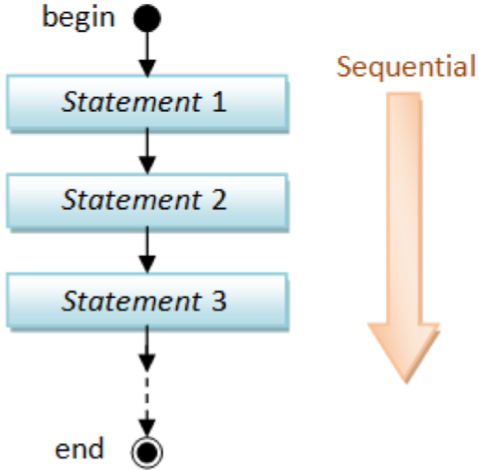
\includegraphics[max size={\textwidth}{\textheight}]{images/chapter-3/sequential-program.png}
  \end{minipage}}
  \fbox{\begin{minipage}{\dimexpr \textwidth-2\fboxsep-2\fboxrule}
    \abovecaptionskip=0pt
    \caption{Sequential program}
  \end{minipage}}
\end{figure}


\subsection*{Evaluation}

\begin{longtabu} to \textwidth {|X[1,l]|X[1,l]|}
    \hline
    \textbf{Advantages} & \textbf{Disadvantages}
    \\ \hline
    \textbf{No additional support required from the programming language}.
    &
    \textbf{Lower processor throughput than concurrent programming} as it cannot benefit from multitasking or concurrent processing.
    \\ \hline
  	\textbf{No additional support required from the operating system} as most old-school operating systems were generally single-threaded and therefore later generations of operating systems typically inherit this functionality.
    &
    \textbf{Multiple computer systems that each have their own CPU may yield a higher cost than multi-CPU systems} as more will be spent on resources, such as the power supply and motherboard, that could be otherwise shared in a multi-CPU system.
    \\ \hline
    &
    \textbf{Lower reliability than a multi-CPU system} because, in the case of the failure of the processor, there is no redundancy.
	\\ \hline
\end{longtabu}


\section*{Concurrent programming}

\subsection*{Definition}

\textbf{Concurrent programming} is the activity of constructing a computer program that takes advantage of concurrency allowed by the use of multiple threads of control.


\subsection*{How it works}

Multiple threads of control allow a given process to perform multiple computations in parallel and to control simultaneous external activities.

The program may be run on both:
\begin{longtabu} to \textwidth { X[1.5,l] X[0.2,l] X[7,l]}
	\textbullet a single-CPU system
	& -- &
	where the computer program will take advantage of multitasking; and
	\\
	\textbullet a multi-CPU system
	& -- &
	where the computer program will take advantage of true parallelism.
\end{longtabu}


\subsection*{Evaluation}

\begin{longtabu} to \textwidth {|X[1,l]|X[1,l]|}
    \hline
    \textbf{Advantages} & \textbf{Disadvantages}
    \\ \hline
    \textbf{Increase processor throughput} due to the use of multitasking in a single-CPU system or parallel processing in a multi-CPU system.
    &
    \textbf{Requires support from the programming language} as it must implement techniques to deal with multitasking on a single-CPU system and/or parallel processing on a multi-CPU system.
    \\ \hline
  	\textbf{A multi-CPU system generally yields a lower cost than using multiple CPUs across multiple computer systems} because the processors share resources such as the power supply and motherboard.
    &
    \textbf{Requires support from the operating system} as it must support multi-threading in order to allow multitasking on a single-CPU system and/or interface and manage multiple CPU units on a multi-CPU system.
    \\ \hline
    \textbf{Increased reliability in a multi-CPU system} because failure of one processor does not affect the other processors, instead the computer system may experience lower performance until fixed.
    &
	\\ \hline
\end{longtabu}


\section{Sequential execution}

\section*{Definition}

Sequential execution is where the execution of threads in a sequential program is executed in sequence/order with no overlapping.


\section*{Order and precedence}

\subsection*{Explanation}

In sequential execution, there is only one possible sequence of execution. This is because a sequential program gives the system strict instructions on the order of executing the statements in the program.


\subsection*{Importance}

For example, a simple hypothetical program could be:
\begin{itemize}
	\item[] P;
	\item[] Q;
	\item[] R;
\end{itemize}

This tells the computer system that the statements must be executed in the order they are written, such that:
\begin{itemize}
	\item P must precede Q; and
	\item Q must precede R.
\end{itemize}


\subsection*{High level}

The importance of the order of precedence can be highlighted by demonstrating this idea in a high-level programming language.

Given the following program written in a high-level language:
\begin{itemize}
	\item[] x = 1;
	\item[] y = x + 1;
	\item[] x = y + 2;
\end{itemize}
it is possible to see that the final values of x and y depend on the order of execution of the statements.


\subsection*{System level}

Given the following program written in a high-level language:
\begin{itemize}
	\item[] x = 1; \textbf{P}
	\item[] y = x + 1; \textbf{Q}
	\item[] x = y + 2; \textbf{R}
\end{itemize}
where each statement is assigned a letter respectively, each statement may be compiled in to several machine instructions.

Statement \textbf{P} is treated as a single machine instruction:
\begin{itemize}
	\item \textbf{P1}: store 1 at the memory address of x.
\end{itemize}

Statement \textbf{Q} is broken in to three machine instructions:
\begin{itemize}
	\item \textbf{Q1}: load the value of x in to a CPU register;
	\item \textbf{Q2}: increment the value in this register by 1; and
	\item \textbf{Q3}: store the value in this register at the memory address of y.
\end{itemize}

Statement \textbf{R} is broken in to three machine instructions:
\begin{itemize}
	\item \textbf{R1}: load the value add of y in to a CPU register;
	\item \textbf{R2}: increment the value in this register by 2; and
	\item \textbf{R3}: store the result at the memory address of x.
\end{itemize}


\section*{The nature of sequential execution}

The execution of statements \textbf{P}, \textbf{Q} and \textbf{R} at the program level (or high-level) as

	\indent \textbf{P} $\rightarrow$ \textbf{Q} $\rightarrow$ \textbf{R}
	
implies that the execution at the system level is as follows

	\indent \textbf{P1} $\rightarrow$ \textbf{Q1} $\rightarrow$ \textbf{Q2} $\rightarrow$ \textbf{Q3} $\rightarrow$ \textbf{R1} $\rightarrow$ \textbf{R2} $\rightarrow$ \textbf{R3},
	
given that \textbf{P} is compiled to a single machine instruction, whilst \textbf{Q} and \textbf{R} are compiled to three machine instructions – as seen on page 40.

Sequential execution has the following assumptions:
\begin{longtabu} to \textwidth { X[1.7,l] X[0.2,l] X[7,l]}
	\textbullet total ordering & -- &
	there is single-threaded computation, and therefore no overlap in the execution of the statements;
	\\
	\textbullet deterministic & -- &
	the same input will always result in the same output; and
	\\
	\textbullet sequence & -- &
	users will specify a strict sequence of steps required in order to achieve a desired goal.
\end{longtabu}
However, this does not apply in many practical applications, for which a sequence of steps is not required.


\section{Introduction to concurrent execution}

\section*{Definition}

\textbf{Concurrent execution} is where the execution of threads in a concurrent program is occurring asynchronously, meaning that the order in which tasks are executed is not predetermined.


\section*{The squares example}

In this hypothetical example, a person desires to have a list with the results of all of the squares (2$^{n}$) from 1 to 100000. 

A group of 100000 people are spilt in to heavily uneven teams and assigned the same task to complete all of the calculations in order to achieve the desired result.

It is given that each calculation takes n amount of time.

\begin{longtabu} to \textwidth {| X[1,l] | X[2,l] | X[1,l] | X[2,l] |}
    \hline
    \multicolumn{2}{|c|}{\textbf{Team 1}}
    & \multicolumn{2}{|c|}{\textbf{Team 2}}
    \\ \hline
    Number of members & 1
    & Number of members & 99999
    \\ \hline
    Strategy &
    One person should complete all of the calculations.
    & Strategy &
    Each member is assigned a number between 1 to 100000.

	Each member should calculate the respective square for the number they are assigned.
	\\ \hline
    Time taken & 100000n
    & Time taken & n
	\\ \hline
\end{longtabu}

This shows that Team 2 was 100000x faster than Team 1. This was because it was possible to decompose the larger task in to smaller sub-tasks and assign each of those tasks to a separate resource, which in this case is one person.

This example forms that basic concept of concurrent execution.


\section*{The nature of concurrent execution}

Concurrent execution dismisses many of the assumptions required for sequential execution (page 41).

Calculations may be carried out without total ordering. As a result, calculations may be carried out in parallel and overlapping is therefore allowed.

In the example above, each individual person in team 2 carried out their operations in sequence.

In the example above, the operations in the whole computation can be viewed as being in partial order. However, the order does not matter here because there is no dependency between the calculations. This is because the output from any given calculation is not required as an input to any other given calculation.

However, in general, concurrent execution is non-deterministic, and therefore the same input generally means different output due to ordering. This is because there are many cases where the order of operation does matter.


\section{Interleaving}

\section*{Why is interleaving required?}

Concurrent execution on a computer system with a multi-core CPU or multiple CPUs can make use of parallel processing in order to run threads asynchronously. However, this is not possible on a computer system with a single-CPU that consists of only one core.

As a result, interleaving is used in order to switch execution between threads.

It is important to note that the operations within each thread are strictly ordered, but the interleaving of the operations are not ordered and are interleaved in an unpredictable order.


\section*{Calculating interleavings}

\subsection*{Formula}

It is possible to calculate the number of interleavings given the formula:
\begin{equation*}
	\text{number of interleavings} = \frac{t_{1} + t_{2} + ... + t_{n}}{t_{1}!t_{2}!...t_{n}}
\end{equation*}
where
\begin{itemize}
	\item $t_{n}$ represents the number of statements/operations in each thread.
\end{itemize}

For example, in a concurrent program that has two threads, the formula may be adjusted to:
\begin{equation*}
	\text{number of interleavings} = \frac{(n + m)!}{n!m!}
\end{equation*}
where
\begin{itemize}
	\item $n$ represents the number of statements/operations in the first thread ($t_{1}$); and
	\item $m$ represents the number of statements/operations in the second thread ($t_{2}$).
\end{itemize}


\subsection*{Example}

A high-level concurrent program may spawn new threads.

\begin{figure}[H]
  \lineskip=-\fboxrule
  \fbox{\begin{minipage}{\dimexpr \textwidth-2\fboxsep-2\fboxrule}
    \centering
    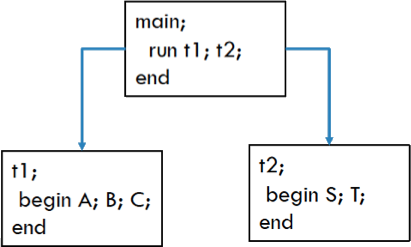
\includegraphics[max size={\textwidth}{\textheight}]{images/chapter-3/concurrent-program-spawing-threads.png}
  \end{minipage}}
  \fbox{\begin{minipage}{\dimexpr \textwidth-2\fboxsep-2\fboxrule}
    \abovecaptionskip=0pt
    \caption{Concurrent program spawning threads $t_{1}$ and $t_{2}$}
  \end{minipage}}
\end{figure}

In this example, the concurrent program spawns the threads $t_{1}$ and $t_{2}$ where:
\begin{longtabu} to \textwidth { X[1.5,l] X[0.2,l] X[3,l]}
	\textbullet $t_{1}$ has three statements & -- &
	A, B and C; and
	\\
	\textbullet $t_{2}$ has two statements & -- &
	S and T.
\end{longtabu}

There are two threads and therefore it is possible to use the adjusted formula to calculate the number of interleavings in this concurrent program:

\begin{equation*}
	\begin{aligned}
		\text{number of interleavings} & = \frac{(n + m)!}{n!m!} \\
		\text{number of interleavings} & = \frac{(3 + 2)!}{3! \times 2!} \\
		\text{number of interleavings} & = \frac{6!}{3! \times 2!} \\
		\text{number of interleavings} & = \frac{6\times5\times4\times3\times2\times1}{(3\times2\times1)\times(2\times1)} \\
		\text{number of interleavings} & = \frac{120}{6\times2} \\
		\text{number of interleavings} & = \frac{120}{12} \\
		\text{number of interleavings} & = 10
	\end{aligned}
\end{equation*}

There are 10 possible interleavings, thus yielding 10 possible different execution sequences.

\begin{figure}[H]
  \lineskip=-\fboxrule
  \fbox{\begin{minipage}{\dimexpr \textwidth-2\fboxsep-2\fboxrule}
    \centering
    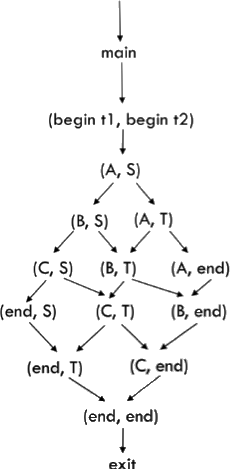
\includegraphics[max size={\textwidth}{\textheight}]{images/chapter-3/possible-execution-sequences.png}
  \end{minipage}}
  \fbox{\begin{minipage}{\dimexpr \textwidth-2\fboxsep-2\fboxrule}
    \abovecaptionskip=0pt
    \caption{Visual representation of the possible execution sequences}
  \end{minipage}}
\end{figure}

A run of the program corresponds to an interleaving sequence. Each interleaving sequence determines a unique sequence of executing the statements. Repeated runs with the same input will likely trace different interleavings.


\subsection*{Growth of interleavings}

The number of interleavings grows extremely quickly given an increase in:
\begin{itemize}
	\item the number of threads in the concurrent program; or
	\item the number of statements/operations in one or more of the concurrent program’s threads.
\end{itemize}

This can be demonstrated by increasing the number of operations in the previous example:
\begin{longtabu} to \textwidth { X[2,l] X[0.2,l] X[3,l]}
	\textbullet $t_{1}$ now has four statements  & -- &
	A, B, C and D; and
	\\
	\textbullet $t_{2}$ now has five statements  & -- &
	S, T, U, V and W.
\end{longtabu}
and therefore:
\begin{equation*}
	\begin{aligned}
		\text{number of interleavings} & = \frac{(n + m)!}{n!m!} \\
		\text{number of interleavings} & = \frac{(4 + 5)!}{4!\times5!} \\
		\text{number of interleavings} & = \frac{9!}{4!\times5!} \\
		\text{number of interleavings} & = \frac{9\times8\times7\times6\times5\times4\times3\times2\times1}{(4\times3\times2\times1)\times(5\times4\times3\times2\times1)} \\
		\text{number of interleavings} & = \frac{362880}{24\times120} \\
		\text{number of interleavings} & = \frac{362880}{2880} \\
		\text{number of interleavings} & = 126
	\end{aligned}
\end{equation*}


\newpage

\section{User and kernel threads}

\section*{User threads}

User threads are created and managed by a user level library, typically without the knowledge of the kernel.

\begin{figure}[H]
  \lineskip=-\fboxrule
  \fbox{\begin{minipage}{\dimexpr \textwidth-2\fboxsep-2\fboxrule}
    \centering
    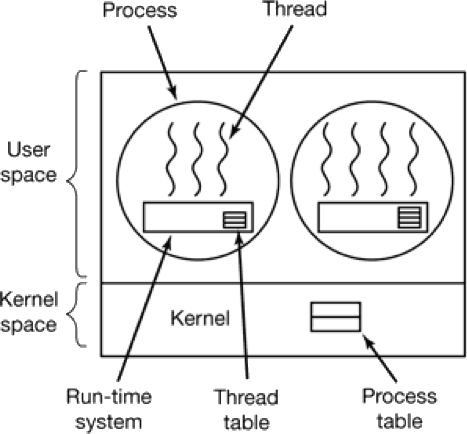
\includegraphics[max size={\textwidth}{\textheight}]{images/chapter-3/user-threads.png}
  \end{minipage}}
  \fbox{\begin{minipage}{\dimexpr \textwidth-2\fboxsep-2\fboxrule}
    \abovecaptionskip=0pt
    \caption{User threads}
  \end{minipage}}
\end{figure}

The diagram shows that:
\begin{itemize}
	\item all of the threads for a given process is present within the user space; and
	\item the thread table is present within the process.
\end{itemize}

User threads are:
\begin{itemize}
	\item fast to create and manage; and
	\item portable to any operating system (OS).
\end{itemize}

If one user thread is blocked, all other threads in the same process are also blocked. For example, in a word processor application, a thread that handles a printing event would block all other threads and therefore prevent the user from interacting with other aspects of the application.

Multi-threaded applications cannot take advantage of parallel execution on computer systems with a multi-core CPU or computer systems with multiple CPUs.


\newpage

\section*{Kernel threads}

Kernel threads are directly managed and supported by the operating system’s (OS’s) kernel.

\begin{figure}[H]
  \lineskip=-\fboxrule
  \fbox{\begin{minipage}{\dimexpr \textwidth-2\fboxsep-2\fboxrule}
    \centering
    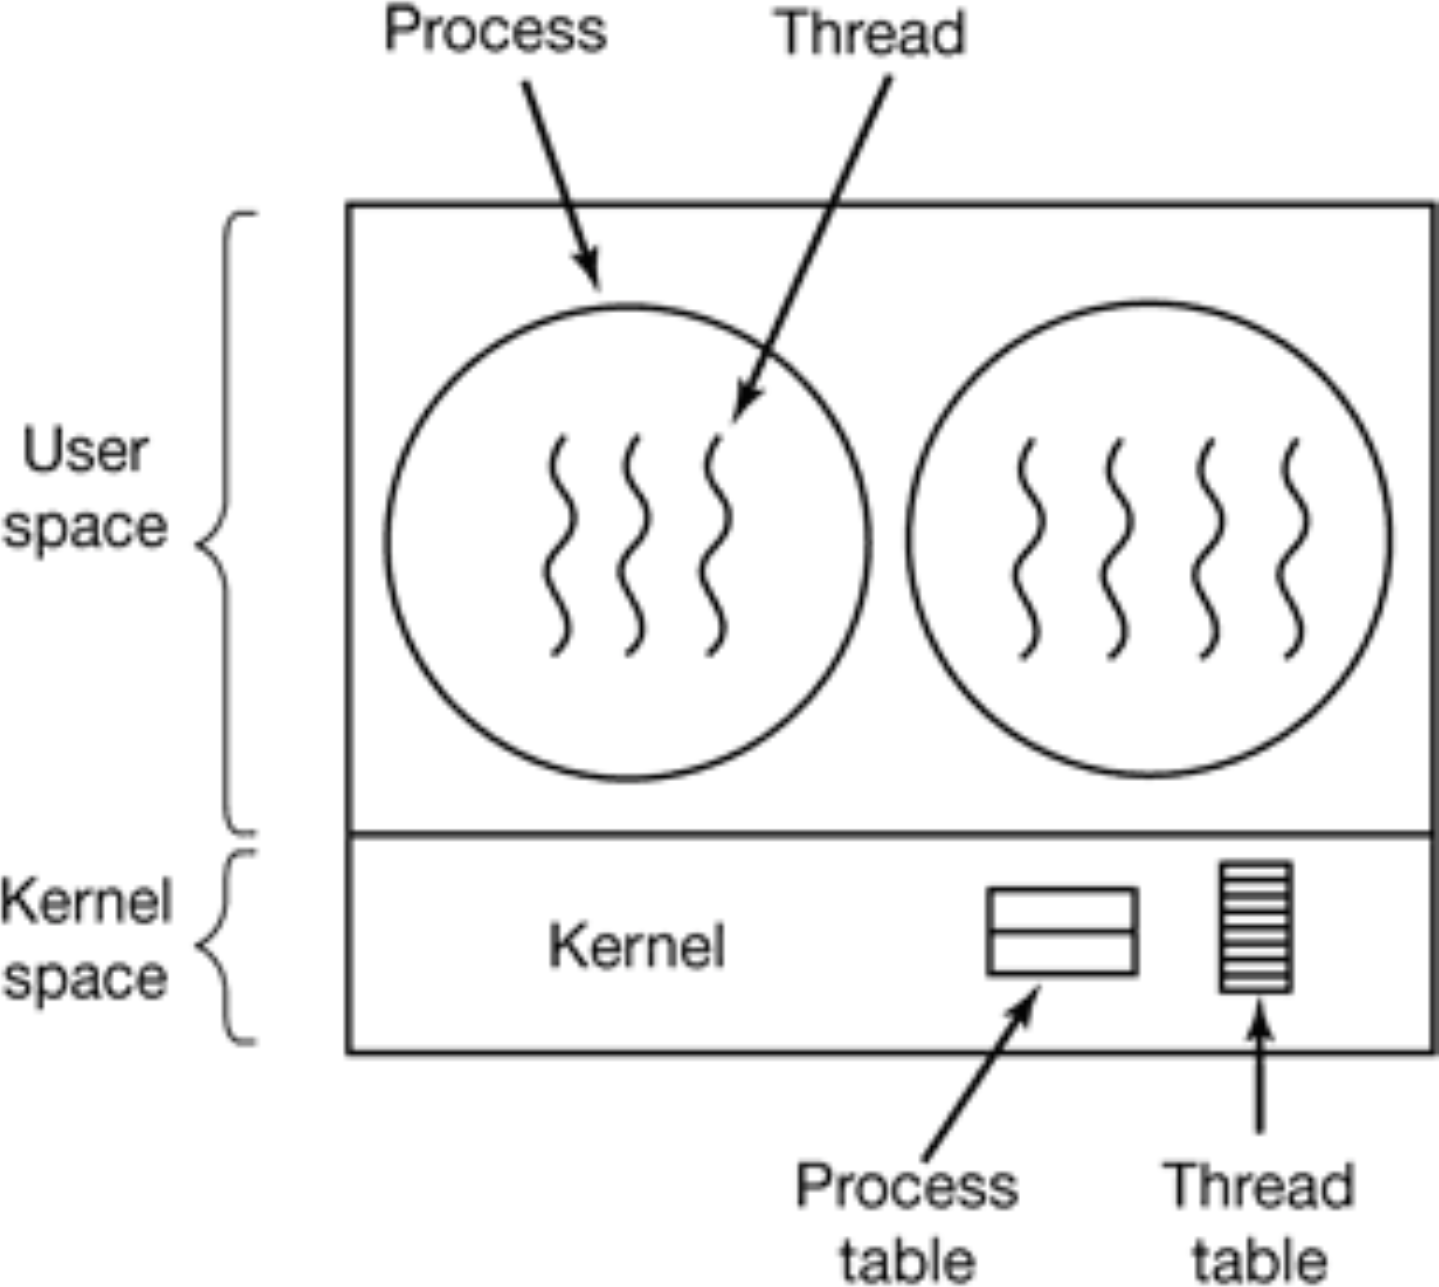
\includegraphics[max size={\textwidth}{\textheight}]{images/chapter-3/kernel-threads.png}
  \end{minipage}}
  \fbox{\begin{minipage}{\dimexpr \textwidth-2\fboxsep-2\fboxrule}
    \abovecaptionskip=0pt
    \caption{Kernel threads}
  \end{minipage}}
\end{figure}

The diagram shows that:
\begin{itemize}
	\item all of the threads for a given process is present within the user space; and
	\item the thread table is present within the kernel space, rather than the process itself or the user space.
\end{itemize}

Kernel threads are:
\begin{itemize}
	\item slower to create and manage than user threads; and
	\item specific to the operating system (OS).
\end{itemize}

If one user thread is blocked, all other threads in the same process are scheduled and not blocked. For example, in a word processor application, a thread that handles a printing event would no longer block all other threads and therefore would allow the user to interacting with other aspects of the application whilst the printing event occurs.

Can take advantage of parallel execution on computer systems with a multi-core CPU or computer systems with multiple CPUs.



\section{Multi-threading models}

\section*{Why is multi-threading mapping required?}

The kernel is generally not aware of the user threads present in a process. Therefore, a thread library must map user threads to kernel threads.


\begin{figure}[H]
  \lineskip=-\fboxrule
  \fbox{\begin{minipage}{\dimexpr \textwidth-2\fboxsep-2\fboxrule}
    \centering
    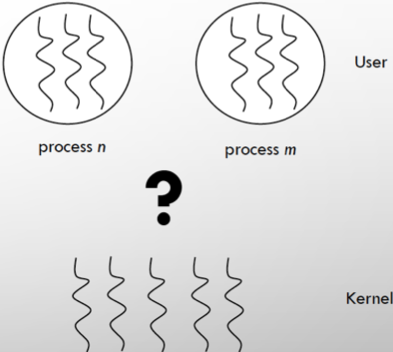
\includegraphics[max size={\textwidth}{\textheight}]{images/chapter-3/multi-threading-mapping.png}
  \end{minipage}}
  \fbox{\begin{minipage}{\dimexpr \textwidth-2\fboxsep-2\fboxrule}
    \abovecaptionskip=0pt
    \caption{Multi-threading mapping}
  \end{minipage}}
\end{figure}

The diagram shows that there must be some relationship between the user threads and the kernel threads. This relationship may defined using different mappings, including:
\begin{itemize}
	\item many-to-one;
	\item one-to-one; and
	\item many-to-many.
\end{itemize}


\section*{Many-to-one mapping}

\subsection*{How it works}

All user threads from each process map to one kernel thread.

\begin{figure}[H]
  \lineskip=-\fboxrule
  \fbox{\begin{minipage}{\dimexpr \textwidth-2\fboxsep-2\fboxrule}
    \centering
    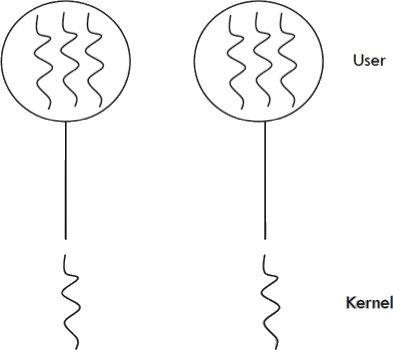
\includegraphics[max size={\textwidth}{\textheight}]{images/chapter-3/many-to-one-mapping.png}
  \end{minipage}}
  \fbox{\begin{minipage}{\dimexpr \textwidth-2\fboxsep-2\fboxrule}
    \abovecaptionskip=0pt
    \caption{Many-to-one mapping}
  \end{minipage}}
\end{figure}


\subsection*{Evaluation}

\begin{longtabu} to \textwidth {|X[1,l]|X[1,l]|}
    \hline
    \textbf{Advantages} & \textbf{Disadvantages}
    \\ \hline
    \textbf{Portable} as there are few system dependencies.
    &
    \textbf{No parallel execution of threads}.
    \\ \hline
    &
    \textbf{No concurrency} as all threads in a process are blocked if another thread is blocked, for example if the thread is waiting for an input/output (I/O) interrupt.
	\\ \hline
\end{longtabu}


\section*{One-to-one mapping}

\subsection*{How it works}

Each user thread maps to a single kernel thread.

\begin{figure}[H]
  \lineskip=-\fboxrule
  \fbox{\begin{minipage}{\dimexpr \textwidth-2\fboxsep-2\fboxrule}
    \centering
    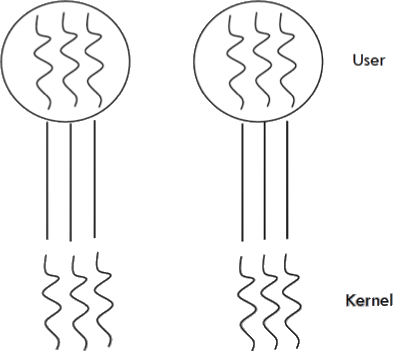
\includegraphics[max size={\textwidth}{\textheight}]{images/chapter-3/one-to-one-mapping.png}
  \end{minipage}}
  \fbox{\begin{minipage}{\dimexpr \textwidth-2\fboxsep-2\fboxrule}
    \abovecaptionskip=0pt
    \caption{One-to-one mapping}
  \end{minipage}}
\end{figure}


\subsection*{Evaluation}

\begin{longtabu} to \textwidth {|X[1,l]|X[1,l]|}
    \hline
    \textbf{Advantages} & \textbf{Disadvantages}
    \\ \hline
    \textbf{Concurrency} as all threads in a process are not blocked if any given thread becomes blocked.
    &
    \textbf{Slow} as there is management overhead because the kernel is involved for every user thread.
    \\ \hline
    \textbf{Performance} as it can take advantage of multiple CPUs.
    &
    \textbf{Restricted} as there is typically a limit on the number of threads.
	\\ \hline
    &
    \textbf{Creating user threads requires the corresponding kernel support}.
	\\ \hline
\end{longtabu}


\section*{Many-to-many mapping}

\subsection*{How it works}

Many user threads multiplex to an equal or smaller number of kernel threads.

\begin{figure}[H]
  \lineskip=-\fboxrule
  \fbox{\begin{minipage}{\dimexpr \textwidth-2\fboxsep-2\fboxrule}
    \centering
    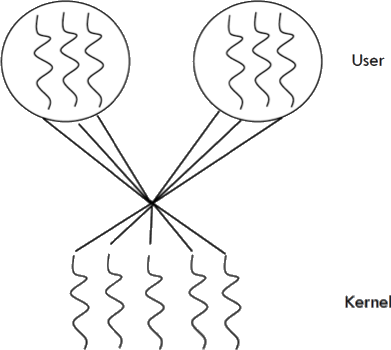
\includegraphics[max size={\textwidth}{\textheight}]{images/chapter-3/many-to-many-mapping.png}
  \end{minipage}}
  \fbox{\begin{minipage}{\dimexpr \textwidth-2\fboxsep-2\fboxrule}
    \abovecaptionskip=0pt
    \caption{Many-to-many mapping}
  \end{minipage}}
\end{figure}

\begin{longtabu} to \textwidth {|X[1,l]|X[1,l]|}
    \hline
    \textbf{Advantages} & \textbf{Disadvantages}
    \\ \hline
    \textbf{Performance} as it can take advantage of multiple CPUs.
    &
    \textbf{Complexity} and therefore implementation difficulties.
    \\ \hline
    \textbf{Flexible} as there is no limit on the number of threads.
    &
	\\ \hline
\end{longtabu}


\newpage

\section{Evaluation of concurrent programming}
\begin{longtabu} to \textwidth {|X[1,l]|X[1,l]|}
    \hline
    \textbf{Advantages} & \textbf{Disadvantages}
    \\ \hline
    \begin{wrapfigure}{l}{4cm}
		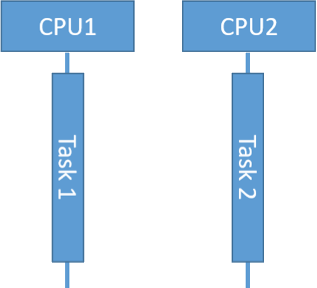
\includegraphics[width=4cm]{images/chapter-3/parallelism.png}
	\end{wrapfigure} 
    \textbf{Parallelism.} It improves the efficiency of program execution in computer systems with multiple CPUs by allows tasks/operations to be split up and executed independently on each CPU.
    &
    \textbf{Debugging complexity} as concurrent programs are non-deterministic and therefore it can be difficult to trace a problem/bug in the code as the same input will generally not result in the same output.  
    \\ \hline
    \begin{wrapfigure}{l}{0.8cm}
		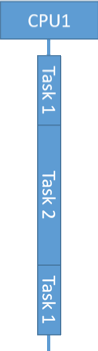
\includegraphics[width=0.8cm]{images/chapter-3/multi-tasking.png}
	\end{wrapfigure}
    \textbf{Multi-tasking.} It improves the utilisation of the CPU in a computer system that only has a single CPU. This allows multiple tasks/operations to run alongside each other and appear to be processed simultaneously.
    &
    \textbf{No protection between threads}.
    \\ \hline
    \textbf{Increases application responsiveness}, for example, in a word processor application one thread could be responsible for responding to user input/output (I/O) while other threads perform tasks in the background.
    &
    \textbf{Concurrent processes must interact with each other} in order to share resources or exchange data.
    \\ \hline
    \textbf{Suited to some applications} as there are some practical applications that are non-deterministic and concurrent as the order of program operations is determined by other external events. This is useful for applications that need to handle multiple events.
    &
    \textbf{Synchronisation must be promoted} in order to determine when, how and with what language abstractions computation events can be synchronised in order to eliminate unacceptable outputs.
    \\ \hline
    &
    \textbf{Distribution must be taken care of} in order to consider how threads can be distributed among a number of CPUs and how one thread is able to interact with another thread on a different CPU.
    \\ \hline
    &
    \textbf{Error-prone}.
	Examples of major concurrent programming errors include:
	\begin{itemize}
		\item Therac-25	- A computerised radiation therapy machine whose errors contributed to accidents causing deaths and serious injuries.
		\item Mars Rover Pathfinder	– Problems with interaction between concurrent tasks caused periodic software resets, thus reducing availability for exploration.
	\end{itemize}
	\\ \hline
\end{longtabu}


\chapter{Synchronisation and Mutual Exclusion}
\label{chap:4}

\section{Race condition}

\section*{Definition}

A \textbf{race condition} describes the competition for resources in a critical section caused by interleaving/thread interference.


\section*{Why do race conditions happen?}

Race conditions occur due to interleaving/thread interference.

\textbf{Interleaving/thread interference} describes an undesired outcome resulting from non-deterministic, concurrent usage of shared resources.

This happens because, in general, concurrent execution is non-deterministic, and therefore the same input generally means different output due to ordering. This is because there are many cases where the order of operation does matter.


\section*{Examples}

\subsection*{Racing for memory access}

A race condition may occur when two threads attempt to access the same location memory, such as registers or RAM, at the same time.

\begin{figure}[H]
  \lineskip=-\fboxrule
  \fbox{\begin{minipage}{\dimexpr \textwidth-2\fboxsep-2\fboxrule}
    \centering
    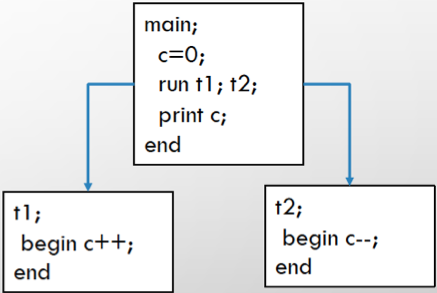
\includegraphics[max size={\textwidth}{\textheight}]{images/chapter-4/concurrent-program-spawning-threads.png}
  \end{minipage}}
  \fbox{\begin{minipage}{\dimexpr \textwidth-2\fboxsep-2\fboxrule}
    \abovecaptionskip=0pt
    \caption{Concurrent program spawning threads $t_{1}$ and $t_{2}$}
  \end{minipage}}
\end{figure}

In this example, the two threads $t_{1}$ and $t_{2}$ manipulate the same variable where:
\begin{itemize}
	\item $t_{1}$ increments the variable $c$; and
	\item $t_{2}$ decrements the variable $c$.
\end{itemize}

As seen before (page 40), each statement may be compiled in to several machine instructions.

The increment ($c++$) instruction is broken in to three machine instructions:
\begin{itemize}
	\item retrieve $c$;
	\item increment retrieved value; and
	\item store result in $c$.
\end{itemize}

The decrement ($c--$) instruction is also broken in to three machine instructions:
\begin{itemize}
	\item retrieve $c$;
	\item decrement retrieved value; and
	\item store result in $c$.
\end{itemize}

As a result, one interleaving possibility is as follows:
\begin{itemize}
	\item $t_{1}$: retrieve $c$;
	\item $t_{2}$: retrieve $c$;
	\item $t_{1}$: increment retrieved value; (result is $1$)
	\item $t_{2}$: decrement retrieved value; (result is $-1$)
	\item $t_{1}$: store result in $c$; ($c$ is now 1)
	\item $t_{2}$: store result in $c$; ($c$ is now -1)
\end{itemize}

This example shows that the race condition has caused the result from thread $t_{1}$ to be lost as it has been overwritten by the result from thread $t_{2}$.


\subsection*{Racing for peripheral access}

A race condition may also occur when two threads attempt to access the same peripheral, such as a printer spooler directory, at the same time.

\begin{figure}[H]
  \lineskip=-\fboxrule
  \fbox{\begin{minipage}{\dimexpr \textwidth-2\fboxsep-2\fboxrule}
    \centering
    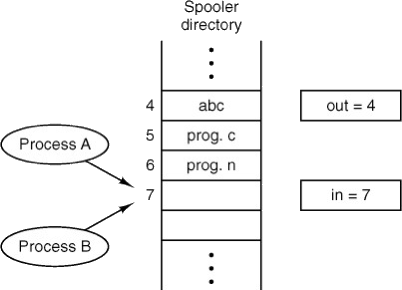
\includegraphics[max size={\textwidth}{\textheight}]{images/chapter-4/printer-spooler-directory.png}
  \end{minipage}}
  \fbox{\begin{minipage}{\dimexpr \textwidth-2\fboxsep-2\fboxrule}
    \abovecaptionskip=0pt
    \caption{Printer spooler directory}
  \end{minipage}}
\end{figure}

In this example, the two processes $A$ and $B$ attempt to access the printer spooler directory at the same time:
\begin{itemize}
	\item the next available printer job slot is $7$;
	\item process $A$ and $B$ access printer job slot $7$ simultaneously;
	\item process $A$ reads printer job slot $7$ and a timer interrupt occurs that causes a context switch to process $B$ before process $A$ has opportunity to store any data;
	\item process $B$ reads printer job slot $7$ and stores its job data and increments the values; and
	\item another timer interrupt occurs that causes a context switch to process $A$ that then stores its job at printer job slot $7$.
\end{itemize}

This example shows that the race condition has caused the job data stored in the printer spooler directory by process $B$ to be lost as it has been overwritten by the job data from process $A$.


\section{Inter-process synchronisation}

\section*{Definition}

\textbf{Inter-process synchronisation} involves techniques that are designed to prevent race conditions and allows threads/processes to share resources.


\section*{Behaviour of threads}

Threads in a computer system may behave in two possible ways:
\begin{itemize}
	\item competing -- two or more processes compete for the same computing resource, for example access to a particular memory cell; or
	\item cooperating -- two or more processes may need to communicate with one another, thus causing information to be passed from one to the other.
\end{itemize}

Inter-process synchronisation is required to manage both threads that are competing and threads that are cooperating.

An operating system (OS) itself contains both threads that are competing and threads that are cooperating.


\section*{How mutual exclusion works}

The solution to preventing race conditions is by implementing mutual exclusion on any given critical section/region.

The \textbf{critical section/region} is code in a process that involves sensitive operations on a shared resource.

\textbf{Mutual exclusion} is the requirement that one thread of execution never enters its critical section/region at the same time that another concurrent thread of execution enters its own critical section/region.

\begin{figure}[H]
  \lineskip=-\fboxrule
  \fbox{\begin{minipage}{\dimexpr \textwidth-2\fboxsep-2\fboxrule}
    \centering
    \includegraphics[max size={\textwidth}{\textheight}]{images/chapter-4/mutual-exclusion.png}
  \end{minipage}}
  \fbox{\begin{minipage}{\dimexpr \textwidth-2\fboxsep-2\fboxrule}
    \abovecaptionskip=0pt
    \caption{Mutual exclusion on critical section/region}
  \end{minipage}}
\end{figure}

When a thread/process enters its critical section/region, no other thread/process may also enter its critical section/region. 

This is demonstrated in the diagram above:
\begin{itemize}
	\item at time interval $T_{1}$, process $A$ enters its critical section/region;
	\item at time interval $T_{2}$, process $B$ attempts to enter its critical section/region;
	\item process $B$ is blocked from entering its critical section/region until process $A$ leaves its critical section/region;
	\item at time interval $T_{3}$, process $A$ leaves its critical section/region and therefore process $B$ is allowed to enter its critical section/region; and
	\item at time interval $T_{4}$, process $B$ leaves its critical section/region.
\end{itemize}

This shown that mutual exclusion is enforced as no two threads/processes are simultaneously inside their critical sections/regions.

For mutual exclusion to be effective:
\begin{itemize}
	\item no assumptions may be made about the speeds or the number of threads/processes;
	\item no threads/processes running outside its critical section/region may block other threads/processes, such that a thread/process that is not in its critical section/region cannot prevent other threads from entering their critical section/region; and
	\item no thread/process should have to wait forever to enter its critical section/region.
\end{itemize}

Mutual exclusion is a major design issue in operating systems (OSs) as consideration must be taken in order to prevent race conditions while maintaining parallelism and efficiency.


\section*{How mutual exclusion is implemented}

Mutual exclusion is implemented using semaphores.

A \textbf{semaphore} is a system tool used for the design of correct synchronisation protocols. This was introduced by Edsger Dijkstra in the 1962/1963. Semaphores are implemented using a variable or abstract data type and are used to control thread/process access to a resource. They are typically integer values that accept only non-negative values.

\begin{figure}[H]
  \lineskip=-\fboxrule
  \fbox{\begin{minipage}{\dimexpr \textwidth-2\fboxsep-2\fboxrule}
    \centering
    \includegraphics[max size={\textwidth}{\textheight}]{images/chapter-4/semaphore-interaction.png}
  \end{minipage}}
  \fbox{\begin{minipage}{\dimexpr \textwidth-2\fboxsep-2\fboxrule}
    \abovecaptionskip=0pt
    \caption{Semaphore interaction on critical section/region}
  \end{minipage}}
\end{figure}

The diagram shows that semaphores allow the CPU to context switch between threads/processes when one becomes blocked.

It is convenient to write entry and exit protocols using a single atomic statement. This statement is atomic and therefore is indivisible, meaning that the statement cannot be interrupted.

As mentioned before, a semaphore, denoted by $S$, is an integer that takes only non-negative values. Only two atomic (indivisible) statements are permitted, as shown below.

\begin{longtabu*} to \textwidth {|X[0.5,l]|X[1,l]|X[1,l]|}
    \hline
	\textbf{Statement} & \textbf{Statement Implementation}
	& \textbf{Usage}
	\\ \hline
	$wait(s)$
	&
	\begin{verbatim}
	wait(s)
	{
	    if ( S > 0 )
	    {
	        S--;
	    }
	}
	\end{verbatim}
	&
	If a thread/process is in its non-critical section/region and wishes to enter its critical section/region, this statement will be performed.

	This means that the thread/process will be blocked until $S = 0$
	evaluates to $True$.
	\\ \hline
	$signal(s)$
	&
	\begin{verbatim}
	signal(s)
	{
	    S++;
	}
	\end{verbatim}
	&
	If a thread/process is in its critical section/region, this statement will be performed.

	This helps to achieve mutual exclusion as it prevents $S = 0$ from evaluating to $True$ until the thread/process has left its critical section/region.
	\\ \hline
\end{longtabu*}

This is a good solution as there is no possibility for a race condition as these statements will always be enforced due to the face that they are atomic (indivisible) statements and cannot be interrupted.


\section{The producer-consumer problem}

\section*{Problem description}

The producer-consumer problem is a classical inter-process communication problem in which:
\begin{itemize}
	\item a producer repeatedly produces items and places them in to a buffer; and
	\item a consumer consumes the items one-by-one by taking them from the buffer.
\end{itemize}

This problem has the following requirements:
\begin{itemize}
	\item the buffer must be assumed to be first in, first out (FIFO);
	\item the producer may produce a new item only at a time when the buffer is not full;
	\item the consumer may consume an item only at a time when the buffer is not empty; and
	\item the process terminates when all items produced are eventually consumed.
\end{itemize}

\begin{figure}[H]
  \lineskip=-\fboxrule
  \fbox{\begin{minipage}{\dimexpr \textwidth-2\fboxsep-2\fboxrule}
    \centering
    \includegraphics[max size={\textwidth}{\textheight}]{images/chapter-4/producer-consumer-problem.png}
  \end{minipage}}
  \fbox{\begin{minipage}{\dimexpr \textwidth-2\fboxsep-2\fboxrule}
    \abovecaptionskip=0pt
    \caption{The producer-consumer problem}
  \end{minipage}}
\end{figure}

The problem arises when attempting to devise a method that is able to:
\begin{itemize}
	\item put the producer to “sleep” when the buffer is full to prevent further items being produced when there is no space in the buffer; and
	\item “wake” the consumer when the buffer is not empty as there is possibility to consumer when the buffer is not empty.
\end{itemize}


\section*{Possible solution}

This problem could be solved by keeping track of the number of items in the buffer.

This could be achieved by implementing loops in the producer class and consumer class.

\newpage

\begin{lstlisting}[title={Producer class}]
LOOP
{
	Produce item i         //produce item
	if ( itemCount == N )  //end of buffer
	{
		sleep(producer);
	}

	Put item i;            // place item in to buffer
	itemCount++;           // increment buffer count
	if ( itemCount == 1)   // buffer nearly empty
	{
		wakeup(consumer);
	}
}
\end{lstlisting}

\begin{lstlisting}[title={Consumer class}]
LOOP
{
	if ( itemCount == 0 )    // buffer empty
	{
		sleep(consumer);
	}

	Remove item j;           // remove item from buffer
	itemCount--;             // decrement buffer count
	if ( itemCount == N-1 )  // buffer has space
	{
		wakeup(producer);
	}
	Consume item j;          // consume item
}
\end{lstlisting}

The loop in the producer class would be running as one thread and the loop in the consumer thread would be running as another thread. These two threads would be running in parallel. As a result, if the threads in the solution are interleaved, a race condition may occur, which in turn, may cause a deadlock.


\subsection*{Deadlocks}

A \textbf{deadlock} occurs when two or more threads wait for each other to finish.

Four conditions must be hold simultaneously in order for a deadlock to occur:
\begin{itemize}
	\item mutual exclusion -- a resource can be assigned to, at most, one process at a time;
	\item hold and wait -- processes holding resources are permitted to request and wait for additional resources;
	\item no pre-emption	 -- resources previously locked cannot be forcefully unlocked by another process, instead they must be released by the holding process; and
	\item circular wait -- there must be a chain of processes, such that each member of the chain is waiting for a resource held by the next member of the chain, as shown in the diagram below.
\end{itemize}

\begin{figure}[H]
  \lineskip=-\fboxrule
  \fbox{\begin{minipage}{\dimexpr \textwidth-2\fboxsep-2\fboxrule}
    \centering
    \includegraphics[max size={\textwidth}{\textheight}]{images/chapter-4/circular-wait.png}
  \end{minipage}}
  \fbox{\begin{minipage}{\dimexpr \textwidth-2\fboxsep-2\fboxrule}
    \abovecaptionskip=0pt
    \caption{Circular wait}
  \end{minipage}}
\end{figure}

A deadlock may occur in the possible solution described previously.

\begin{figure}[H]
  \lineskip=-\fboxrule
  \fbox{\begin{minipage}{\dimexpr \textwidth-2\fboxsep-2\fboxrule}
    \centering
    Consumer reads $itemCount = 0$ and it evaluates to $True$, and therefore $sleep(consumer)$ needs to be called.
    
	$\downarrow$
	
	Just before $sleep(consumer)$ is called, the consumer is interrupted by a timer interrupt and the producer is resumed.
	
	$\downarrow$
	
	The producer places an item in to the buffer, such that $itemCount = 1$.
	
	$\downarrow$
	
	The producer tries to perform $wakeup(consumer)$ however, the consumer is already in “wakeup” mode. As a result, the call to $wakeup(consumer)$ is missed.
	
	$\downarrow$
	
	When the consumer resumes, it will call $sleep(consumer)$ and get trapped in “sleep” mode.
	
	$\downarrow$
	
	The producer will continue placing items in the buffer and call $sleep(producer)$ when the buffer is full.
	
	$\downarrow$
	
	There is now a deadlock as both threads are waiting for a $wakeup$ call from each other.
  \end{minipage}}
  \fbox{\begin{minipage}{\dimexpr \textwidth-2\fboxsep-2\fboxrule}
    \abovecaptionskip=0pt
    \caption{Possible deadlock}
  \end{minipage}}
\end{figure}

This possible deadlock shows that another solution is required to effectively solve the producer-consumer problem.


\section*{Solving the problem using semaphores}

It is assumed that
\begin{lstlisting}
ItemsReady = 0
SpacesLeft = N  //size of buffer
\end{lstlisting}

\begin{lstlisting}[title={Producer class}]
LOOP
{
	Produce item i      // produce item
	Wait(SpacesLeft)    // decrement semaphore

	Put item i;         // place item in to buffer
	Signal(ItemsReady)  // increment
}
\end{lstlisting}

\begin{lstlisting}[title={Consumer class}]
LOOP
{
	Wait(ItemsReady)    // decrement semaphore

	Get item j;         // remove item from buffer
	Signal(SpacesLeft)  // increment semaphore
	Consume item i;     // consume item
}
\end{lstlisting}

If this solution uses semaphores correctly, then
\begin{equation*}
	\begin{aligned}
		\text{N = SpacesLeft + ItemsReady}
	\end{aligned}
\end{equation*}

as the producer will always be placing items in to the buffer when there are spaces available in the buffer.

However, this solution does not consider situations in which there are multiple producers and/or multiple consumers.


\newpage

\section*{The multiple producer-consumer problem}

\subsection*{Problem description}

The multiple producer-consumer problem is a classical inter-process communication problem in which:
\begin{itemize}
	\item multiple producer repeatedly produces items and places them in to a buffer; and
	\item multiple consumer consumes the items one-by-one by taking them from the buffer.
\end{itemize}

As with the previous producer-consumer problem, this problem has the following requirements:
\begin{itemize}
	\item the buffer must be assumed to be first in, first out (FIFO);
	\item the producers may produce a new item only at a time when the buffer is not full;
	\item the consumers may consume an item only at a time when the buffer is not empty; and
	\item the process terminates when all items produced are eventually consumed.
\end{itemize}

\begin{figure}[H]
  \lineskip=-\fboxrule
  \fbox{\begin{minipage}{\dimexpr \textwidth-2\fboxsep-2\fboxrule}
    \centering
    \includegraphics[max size={\textwidth}{\textheight}]{images/chapter-4/multiple-producer-consumer-problem.png}
  \end{minipage}}
  \fbox{\begin{minipage}{\dimexpr \textwidth-2\fboxsep-2\fboxrule}
    \abovecaptionskip=0pt
    \caption{The multiple producer-consumer problem}
  \end{minipage}}
\end{figure}

The problem arises when attempting to devise a method that is able to manage:
\begin{itemize}
	\item two producers placing items in to the same slot in the buffer; and
	\item two consumers removing items from the same slot in the buffer.
\end{itemize}
This is similar to the problem discussed in the printer spooler example (page n).

A race condition may also occur when producers attempt to access a variable at the same time.

To demonstrate the race condition, it is necessary to consider the following possible interleaving of the threads/processes:
\begin{itemize}
	\item two producers access the $SpacesLeft$ variable at the same time, which corresponds to decrementing the semaphore;
	\item both producers get the same next empty slot in the buffer at the same time; and
	\item both producers write in to the same slot.
\end{itemize}

This example shows that the race condition has caused the data stored in the buffer slot by the first producer to be lost as it has been overwritten by the data stored in the buffer slot by the second producer.

In order to ensure mutual exclusion when multiple users are involved, an additional semaphore must be introduced.


\subsection*{Mutex}

A \textbf{mutex} (or \textbf{binary semaphore}) is a semaphore with ownership that can only be released by its owner and is initially set to $1$.


\subsection*{Problem solution}

It is now possible to construct a solution, using a mutex (or binary semaphore), that will ensure mutual exclusion even when there are multiple producers and/or multiple consumers.

It is assumed that
\begin{lstlisting}
ItemsReady = 0
SpacesLeft = N  //size of buffer
\end{lstlisting}

\begin{lstlisting}[title={Producer class}]
LOOP
{
	Produce item i      // produce item
	Wait(SpacesLeft)    // decrement semaphore
	Wait(BusyBuffer)    // mutex

	Put item i;         // place item in to buffer
	Signal(BusyBuffer)  // release mutex
	Signal(ItemsReady)  // increment
}
\end{lstlisting}

\begin{lstlisting}[title={Consumer class}]
LOOP
{
	Wait(ItemsReady)    // decrement semaphore
    Wait(BusyBuffer)    // mutex

    Get item j;         // remove item from buffer
    Signal(SpacesLeft)  // increment semaphore
    Signal(BusyBuffer)  // release mutex
    Consume item i;     // consume item
}
\end{lstlisting}

The mutex $BusyBuffer$ has ownership and therefore can only be incremented/decremented by the same thread/process.

The order in which semaphores are incremented and decremented is essential. This can be demonstrated by inspecting the effect of switching around two statements in the Consumer class:
\begin{lstlisting}
Wait(ItemsReady)  //decrement semaphore
Wait(BusyBuffer)  //mutex
...
Wait(BusyBuffer)  //mutex
Wait(ItemsReady)  //decrement semaphore
\end{lstlisting}

This switching would cause …


\section{The dining philosophers problem}

\section*{Problem description}

The dining philosophers problem is a classical inter-process communication problem in which:
\begin{itemize}
	\item five philosophers are seated around a circular table eating and thinking; and
	\item each philosopher has a plate of spaghetti that they can eat with forks.
\end{itemize}

This problem has the following requirements:
\begin{itemize}
	\item the life of a philosopher consists of only alternating periods of eating and thinking;
	\item between each pair of plates is one fork;
	\item each philosopher needs two forks to eat the spaghetti; and
	\item no two philosophers may hold the same fork simultaneously.
\end{itemize}

\begin{figure}[H]
  \lineskip=-\fboxrule
  \fbox{\begin{minipage}{\dimexpr \textwidth-2\fboxsep-2\fboxrule}
    \centering
    \includegraphics[max size={\textwidth}{\textheight}]{images/chapter-4/layout-of-table.png}
  \end{minipage}}
  \fbox{\begin{minipage}{\dimexpr \textwidth-2\fboxsep-2\fboxrule}
    \abovecaptionskip=0pt
    \caption{Layout of table}
  \end{minipage}}
\end{figure}

The problem arises when attempting to devise a method that is able to:
\begin{itemize}
	\item allow each philosopher to have alternating periods of eating and thinking; and
	\item not result in a deadlock.
\end{itemize}

It could be said that the problem requirement for each philosopher to need two forks to eat the spaghetti is somewhat artificial. As a result, we can substitute the spaghetti for rice and substitute chopsticks for forks.

The problem now has the following updated requirements:
\begin{itemize}
	\item the life of a philosopher consists of only alternating periods of eating and thinking;
	\item between each pair of plates is one chopstick;
	\item each philosopher needs two chopsticks to eat the rice; and
	\item no two philosophers may hold the same chopstick simultaneously.
\end{itemize}

\begin{figure}[H]
  \lineskip=-\fboxrule
  \fbox{\begin{minipage}{\dimexpr \textwidth-2\fboxsep-2\fboxrule}
    \centering
    \includegraphics[max size={\textwidth}{\textheight}]{images/chapter-4/updated-layout-of-table.png}
  \end{minipage}}
  \fbox{\begin{minipage}{\dimexpr \textwidth-2\fboxsep-2\fboxrule}
    \abovecaptionskip=0pt
    \caption{Updated layout of table}
  \end{minipage}}
\end{figure}


\section*{Problem solutions}

\subsection*{Problem solution 1}

This problem can be solved using semaphores, using the following assumptions:
\begin{itemize}
	\item each philosopher is a different thread with a unique ID;
	\item one semaphore is implemented per chopstick; and
	\item chopsticks are identified by using the unique ID of a philosopher.
\end{itemize}

As chopsticks are identified by using the unique ID of a philosopher, it could be that:
\begin{itemize}
	\item the chopstick to the left of a given philosopher is $chopstick[i]$; and
	\item the chopstick to the right of a given philosopher is $chopstick[(i-1) + N) \% N].$
\end{itemize}
where $i$ is the ID of the philosopher and $N$ is the number of philosophers.

The identification of the chopsticks works as demonstrated by using Philosopher 1 as an example.

\begin{figure}[H]
  \lineskip=-\fboxrule
  \fbox{\begin{minipage}{\dimexpr \textwidth-2\fboxsep-2\fboxrule}
    \centering
    \includegraphics[max size={\textwidth}{\textheight}]{images/chapter-4/philosopher-1.png}
  \end{minipage}}
  \fbox{\begin{minipage}{\dimexpr \textwidth-2\fboxsep-2\fboxrule}
    \abovecaptionskip=0pt
    \caption{Philosopher 1}
  \end{minipage}}
\end{figure}

The diagram shows that:
\begin{itemize}
	\item the chopstick to the left of Philosopher 1 is $chopstick[1]$; and
	\item the chopstick to the right of Philosopher 1 is $chopstick[0]$.
\end{itemize}

Using this example, it is possible to validate the chopstick identification formulas discussed before.

Given that $i = 1$ for Philosopher 1 and that $N = 5$ as there are five philosophers in total,
\begin{equation*}
	\begin{aligned}
		\text{left} & = \text{chopstick[i]} \\
		\text{left} & = \text{chopstick[1]} \\
		\text{right} & = \text{chopstick[(i-1) + N) \% N]} \\
		\text{right} & = \text{chopstick[(1-1) + 5) \% 5]} \\
		\text{right} & = \text{chopstick[(0 + 5) \% 5]} \\
		\text{right} & = \text{chopstick[5 \% 5]} \\
		\text{right} & = \text{chopstick[0]} \\
	\end{aligned}
\end{equation*}
This shows that the chopstick identification formulas work for Philosopher 1.

\begin{lstlisting}[title={Producer class}]
LOOP
{
	think();
	wait(chopstick[left]);     // take left chopstick
	wait(chopstick[right]);    // take right chopstick
	eat();
	signal(chopstick[left]);   // release left chopstick
	signal(chopstick[right]);  // release right chopstick
}
\end{lstlisting}

However, this solution has the possibility to cause a race condition.

This can be demonstrated in the situation where all five philosophers wish to eat at the same time and therefore all take their left chopsticks:
\begin{itemize}
	\item Philosopher 0 takes $chopstick[left]$;
	\item Philosopher 1 takes $chopstick[left]$;
	\item Philosopher 2 takes $chopstick[left]$;
	\item Philosopher 3 takes $chopstick[left]$; and
	\item Philosopher 4 takes $chopstick[left]$.
\end{itemize}

This causes a race condition as:
\begin{itemize}
	\item each philosopher will now be waiting to take $chopstick[right]$;
	\item no philosopher can take $chopstick[right]$ as this chopstick is the subsequent philosopher’s $chopstick[left]$ and this has already been taken; and
	\item no philosopher can perform their $eat$ function and therefore no chopsticks will be released as the $signal$ functions are only performed after the $eat$ function has completed.
\end{itemize}

This shows that, if the threads in the solution are interleaved, a race condition may occur. In this case, a circular wait is caused and therefore there is a deadlock.


\subsection*{Possible solution 2}

As shown in the multiple producer-consumer problem, a mutex (or binary semaphore) can be introduced to prevent this deadlock.

\begin{lstlisting}[title={Producer class}]
LOOP
{
	think();
	wait(busy);                // mutex
	wait(chopstick[left]);     // take left chopstick
	wait(chopstick[right]);    // take right chopstick
	eat();
	signal(chopstick[left]);   // release left chopstick
	signal(chopstick[right]);  // release right chopstick
	signal(busy);              // release mutex
}
\end{lstlisting}

This solves the deadlock as the mutex (or binary semaphore) signals the critical section/region and prevents other philosophers from attempting to take a chopstick that is currently in use by another philosopher.

Although this solution is deadlock-free, it has a performance bug. The mutex means that only one philosopher can be eating at any instant and, with five chopsticks available, it should be possible to allow two philosophers to eat at the same time. As a result, there are more efficient solutions to this problem that achieve maximum parallelism.

\subsection*{Final revision solution}

This solution is deadlock-free and allows the maximum parallelism for an arbitrary number of philosophers.

\begin{lstlisting}[title={Producer class}]
#define N         5                // number of philosophers
#define LEFT      (i + N - 1) % N  // ID of i's left neighbour
#define RIGHT     (i + 1) % N      // ID of i's right neighbour
#define THINKING  0                // philosopher is thinking
#define HUNGRY    1                // philosopher is trying to acquire
                                   // chopsticks
#define EATING    2                // philosopher is eating

typedef int semaphore              // semaphores are a special kind of
                                   // integer
int state[N];                      // array to keep track of philosopher's
                                   // state             
semaphore mutex = 1;               // mutual exclusion for critical regions
semaphore s[N];                    // one semaphore per philosopher

// i: philosopher unique ID, from 0 to N-1
void philosopher (int i)
{
	while (TRUE)                   // repeat indefinitely
	{
		think();                   // philosopher is thinking
		take_chopsticks(i);        // acquire two chopsticks or be blocked
		eat();                     // philosopher is eating
		put_chopsticks(i);         // place both chopsticks back on the table
	}
}

// i: philosopher unique ID, from 0 to N-1
void take_chopsticks(int i)
{
	wait(&mutex);                  // enter critical section/region
	state[i] = HUNGRY;             // record fact that philosopher i is hungry
	test(i);                       // attempt to acquire two chopsticks
	signal(&mutex);                // exit critical section/region
	wait(&s[i]);                   // block if chopsticks were not acquired
}

// i: philosopher unique ID, from 0 to N-1
void put_chopsticks(int i)
{
	wait(&mutex);                  // enter critical section/region
	state[i] = THINKING;           // record fact that philosopher i is
	                               // thinking
	test(LEFT);                    // check if left neighbour can now eat
	test(RIGHT);                   // check if right neighbour can now eat
	signal(&mutex);                // exit critical section/region
}

// i: philosopher unique ID, from 0 to N-1
void test(int i)
{
	if (state[i] == HUNGRY && state[LEFT] != EATING
		&& state[RIGHT] != EATING)
	{
		state[i] = EATING;         // record fact that philosopher i is hungry
		signal(&s[i]);             // exit critical section/region
	}
}
\end{lstlisting}

This solution uses the array state to keep track of whether a philosopher is:
\begin{itemize}
	\item eating;
	\item thinking; or
	\item hungry (trying to acquire chopsticks).
\end{itemize}

This represents an array of semaphores and each philosopher has its own $state$ array. This enables hungry philosophers to be blocked if the required chopsticks are currently busy.

A philosopher may move in to eating state only if neither neighbouring philosopher is eating. For example, Philosopher 1 cannot enter eating state if:
\begin{itemize}
	\item Philosopher 0 is currently in eating state; or
	\item Philosopher 2 is currently in eating state.
\end{itemize}


\chapter{Memory Management}

\section{Memory hierarchy}

\section*{Definition}

The \textbf{memory hierarchy} separates computer storage into a hierarchy based on response time. A computer system is usually composed by a layered memory system


\section*{Diagram}

\begin{figure}[H]
  \lineskip=-\fboxrule
  \fbox{\begin{minipage}{\dimexpr \textwidth-2\fboxsep-2\fboxrule}
    \centering
    \includegraphics[max size={\textwidth}{\textheight}]{images/chapter-5/memory-hierarchy-pyramid.png}
  \end{minipage}}
  \fbox{\begin{minipage}{\dimexpr \textwidth-2\fboxsep-2\fboxrule}
    \abovecaptionskip=0pt
    \caption{Memory hierarchy pyramid}
  \end{minipage}}
\end{figure}

Higher layers correspond to faster devices that:
\begin{itemize}
	\item have lower capacity;
	\item require more power and generate more heat; and
	\item are more expensive.
\end{itemize}

Lower layers correspond to slower devices that:
\begin{itemize}
	\item have higher capacity;
	\item require less power and generate less heat; and
	\item are cheaper.
\end{itemize}

The temporary storage areas can be described as volatile; the data does not persist after power-down.

The permanent storage areas can be described as non-volatile; the data persists after power-down.


\section{Primary memory}

\section*{Definition}

\textbf{Primary memory} is volatile, meaning that the data contained within does not persist after power-down, and stores data and instructions for use by the CPU in currently running processes.


\section*{Registers}

\begin{longtabu} to \textwidth {| X[1,l] | X[6,l] |}
    \hline
    \textbf{Size} & Very small.
	\\ \hline
	\textbf{Speed} & Extremely fast.
	\\ \hline
	\textbf{Purpose} & Individual containers for single values.
	
	Almost all computers load data from a memory lower in the hierarchy into registers, where it is used for arithmetic operations and is manipulated or tested by machine instructions.
	\\ \hline
	\textbf{Location} & Inside the CPU.
	\\ \hline
\end{longtabu}

Registers are typically referred to by “name” (i.e. individual identifying code), not by address, as happens with other types of memory.

\begin{figure}[H]
  \lineskip=-\fboxrule
  \fbox{\begin{minipage}{\dimexpr \textwidth-2\fboxsep-2\fboxrule}
    \centering
    \includegraphics[max size={\textwidth}{\textheight}]{images/chapter-5/registers.png}
  \end{minipage}}
  \fbox{\begin{minipage}{\dimexpr \textwidth-2\fboxsep-2\fboxrule}
    \abovecaptionskip=0pt
    \caption{Registers}
  \end{minipage}}
\end{figure}

There are two main types of registers:
\begin{itemize}
	\item generic registers -- allow the CPU to temporarily store data on which it will perform operations, and consequently data that results from those operations; and
	\item specialised registers -- manipulated in mostly the same fashion as generic registers but are used for specialised purposes.
\end{itemize}

Specialised registers include:
\begin{itemize}
	\item Instruction Register (IR) -- holds the instruction currently being executed;
	\item Memory Data Register (MDR) -- holds the piece of data that has been fetched from memory;
	\item Memory Address Register (MAR) -- holds the address of the next piece of memory to be fetched;
	\item Program Counter (PC) -- holds the location of the next instruction to be fetched from memory and is automatically incremented between supplying the address of the next instruction and the instruction being executed; and
	\item Accumulator (ACCU) -- used as the default location to store any calculations performed by the arithmetic and logic unit.
\end{itemize}

Generic registers are available to store any transient data required by the program.

For example, when a program is interrupted its state, the values stored in the specialised registers may be saved into the generic registers, ready for recall when the program is ready to start again.

In general, the more registers a CPU has available, the faster it can work.


\section*{Cache memory}

\begin{longtabu} to \textwidth {| X[1,l] | X[6,l] |}
    \hline
    \textbf{Size} & Small (KB/MB).
	\\ \hline
	\textbf{Speed} & Fast.
	\\ \hline
	\textbf{Purpose} & Serves as an intermediary between main memory and the registers.
	
	When data or instructions are fetched from main memory, they are copied to the cache for further use, and therefore, reduce the average cost (time or energy) to access data from the main memory.
	\\ \hline
	\textbf{Location} & Inside the CPU.
	\\ \hline
\end{longtabu}

\begin{figure}[H]
  \lineskip=-\fboxrule
  \fbox{\begin{minipage}{\dimexpr \textwidth-2\fboxsep-2\fboxrule}
    \centering
    \includegraphics[max size={\textwidth}{\textheight}]{images/chapter-5/cache-memory.png}
  \end{minipage}}
  \fbox{\begin{minipage}{\dimexpr \textwidth-2\fboxsep-2\fboxrule}
    \abovecaptionskip=0pt
    \caption{Cache memory}
  \end{minipage}}
\end{figure}

Modern computers typically have a sub-hierarchy of cache memories (L1, L2, L3, L4, etc.), for example:
\begin{itemize}
	\item level 1 cache (L1)	 -- very fast and small size (2KB - 64KB); and
	\item level 2 cache (L2)	 -- fast and medium size (256KB – 2MB).
\end{itemize}


\section*{Main memory}

\begin{longtabu} to \textwidth {| X[1,l] | X[6,l] |}
    \hline
    \textbf{Size} & Medium (MB/GB).
	\\ \hline
	\textbf{Speed} & Fast.
	\\ \hline
	\textbf{Purpose} & Stores data and machine code currently being used.
	\\ \hline
	\textbf{Location} & Motherboard, connected to the CPU by a bus.
	\\ \hline
\end{longtabu}

\begin{figure}[H]
  \lineskip=-\fboxrule
  \fbox{\begin{minipage}{\dimexpr \textwidth-2\fboxsep-2\fboxrule}
    \centering
    \includegraphics[max size={\textwidth}{\textheight}]{images/chapter-5/main-memory.png}
  \end{minipage}}
  \fbox{\begin{minipage}{\dimexpr \textwidth-2\fboxsep-2\fboxrule}
    \abovecaptionskip=0pt
    \caption{Main memory}
  \end{minipage}}
\end{figure}

Main memory is typically a random-access memory (RAM) device. These devices allow data items to be read from or written to in almost the same amount of time, irrespective of the physical location of the data.


\section{Secondary memory}

\section*{Definition}

\textbf{Secondary memory} is a non-volatile and persistent store of data, which is used for items such as user files, programs and the operating system.


\section*{Magnetic -- Hard-Disk Drive (HDD)}

\subsection*{Description}

A \textbf{Hard-Disk Drive (HDD)} contains rotating platters which are coated with magnetic material. This contains ferrous particles, containing iron, which are polarised to become either a north or south state; these states can correspond to either a 0 or a 1.

The platters spin at speeds of up to 10,000 revolutions per minute (RPM) and a drive head moves across the platters to access different tracks and sectors. Data is read from or written to the platters as it passes under the drive head. When no operations are being performed, the drive head is parked to the side of the platters to prevent damage from movement.

There may be several platters and several drive heads.

\begin{longtabu} to \textwidth {| X[1,l] | X[6,l] |}
    \hline
    \textbf{Size} & xxx’GB and x’TB.
	\\ \hline
	\textbf{Speed} & Medium.
	\\ \hline
	\textbf{Purpose} & Consumer desktop computer system secondary storage.
	\\ \hline
	\textbf{Reliability} & Prone to drop damage as it has moving parts and magnetic fields.
	\\ \hline
\end{longtabu}

\subsection*{Evaluation}

\begin{longtabu} to \textwidth {| X[1,l] | X[1,l] |}
    \hline
    \textbf{Advantages} & \textbf{Disadvantages}
	\\ \hline
	\textbf{Large storage capacity}. & \textbf{Relatively slow read and write speeds} because the disk head must physically move to the location of the data on the platter.
	\\ \hline
	\textbf{Affordable large capacities}, HDDs are available in large storage capacities at relatively low prices. & \textbf{Can be loud} because there are moving parts, such as the platters and disk head, which generate noise.
	\\ \hline
	& \textbf{Low reliability} because they are prone to drop damage, due to their moving parts, magnetic fields.
	\\ \hline
	& \textbf{Relatively large form factor} since there must be room to enclose the platters and disk heads.
	\\ \hline
\end{longtabu}


\section*{Magnetic -- Magnetic tape}

\subsection*{Description}

A \textbf{magnetic tape} is a reel of tape which is coated with a magnetic material. This contains ferrous particles, containing iron, which are polarised to become either a north or south state; these states can represent either a 1 or a 0.

The data is accessed using serial access; this is where a tape reader starts at the beginning of the tape and “fast forwards” to the portion of the tape containing the required data.

\begin{longtabu} to \textwidth {| X[1,l] | X[6,l] |}
    \hline
    \textbf{Size} & xxx’GB and x’TB.
	\\ \hline
	\textbf{Speed} & Slow.
	\\ \hline
	\textbf{Purpose} & Server backup storage.
	\\ \hline
	\textbf{Reliability} & Prone to magnetic fields.
	\\ \hline
\end{longtabu}


\newpage

\subsection*{Evaluation}

\begin{longtabu} to \textwidth {| X[1,l] | X[1,l] |}
    \hline
    \textbf{Advantages} & \textbf{Disadvantages}
	\\ \hline
	\textbf{Large storage capacity}. & \textbf{Relatively slow read and write speeds} because it uses serial data access.
	\\ \hline
	\textbf{Affordable large capacities}, magnetic tapes are available in high capacities at relatively low prices & \textbf{Low reliability} because they are prone to magnetic fields.
	\\ \hline
	& \textbf{Requires specialist equipment} to read the data on the tape, known as a tape reader.
	\\ \hline
\end{longtabu}


\section*{Flash -- Solid-State Drive (SSD)}

\subsection*{Description}

A \textbf{Solid-State Drive (SSD)} contains millions of NAND flash memory cells and a controller which manages pages and blocks of memory.

Each NAND flash memory cell delivers a current along the bit and word lines to activate the flow of electrons from the source towards the drain. The current on the word line is strong enough to push a few electrons across an insulated oxide layer into a floating gate. The charge in the flowing gate is measured: if there is some charge, where there are some electrons flowing, a 1 is represented; and if there is no charge, where there are no electrons flowing, a 0 is represented.

\begin{longtabu} to \textwidth {| X[1,l] | X[6,l] |}
    \hline
    \textbf{Size} & xx’GB and xxx’GB.
	\\ \hline
	\textbf{Speed} & Very fast.
	\\ \hline
	\textbf{Purpose} & Portable device secondary storage, such as smartphones and laptops.
	\\ \hline
	\textbf{Reliability} & Less prone to drop damage as there are no moving parts, limited write cycles before damage.
	\\ \hline
\end{longtabu}

Flash drives and SD cards also use solid-state technologies. They are often used for portable storage; for example, flash drives may be used for transferring documents and SD cards may be used to storage images in a camera.


\subsection*{Evaluation}

\begin{longtabu} to \textwidth {| X[1,l] | X[1,l] |}
    \hline
    \textbf{Advantages} & \textbf{Disadvantages}
	\\ \hline
	\textbf{Fast read and write speeds} because the data can be accessed directly on the drive using electrical currents. & \textbf{Expensive large capacities}, SSDs are more expensive than other storage options.
	\\ \hline
	\textbf{Available in different form factors}, such as USB memory sticks and SD cards. & \textbf{Low durability} because they have a finite number of read and write operations which can be performed before the performance of the drive beings to downgrade due the discharge of its electrons.
	\\ \hline
	\textbf{High reliability} because there are no moving parts. &
	\\ \hline
	\textbf{Silent operation} because there are no moving parts. &
	\\ \hline
\end{longtabu}


\section*{Optical -- Optical disk}

\subsection*{Description -- Optical disk}

An \textbf{optical disk} works by using:
\begin{itemize}
	\item a high-powered laser to change the properties of its surface to make them less reflective, by a process called “burning”; and
	\item a low-powered laser to read the disk by shining light onto the surface and a sensor is used to measure the amount of light that is reflected back.
\end{itemize}

There are multiple types of optical disks, including:
\begin{itemize}
	\item CD-ROM;
	\item CD-RW;
	\item DVD-RW; and
	\item Bluray.
\end{itemize}

\subsection*{Description -- CD-ROM}

A \textbf{CD-ROM (read only Compact Disk)} is pressed during is manufacture and has pits, where the surface has been depressed, and lands, where the surface has not been depressed.

When the low-powered laser is shone on the surface:
\begin{itemize}
	\item the start or end of a pit, the light is scattered and not reflected very well –- this is used to represent a 0; and
	\item a land, the light is not scattered and reflected normally -– this is used to represent a 1.
\end{itemize}

\begin{longtabu} to \textwidth {| X[1,l] | X[6,l] |}
    \hline
    \textbf{Size} & xxx'MB.
	\\ \hline
	\textbf{Speed} & Slow.
	\\ \hline
	\textbf{Purpose} & Commercial music distribution.
	\\ \hline
	\textbf{Reliability} & Prone to scratches and cracks.
	\\ \hline
\end{longtabu}


\subsection*{Description -- CD-RW}

A \textbf{CD-RW (re-writable Compact Disk)} uses a laser and a magnet to heat a spot on the disk. When the spot is heated the magnetic orientation is changed to represent a 0 or a 1 before the magnet is cooled.

\begin{longtabu} to \textwidth {| X[1,l] | X[6,l] |}
    \hline
    \textbf{Size} & xxx'MB.
	\\ \hline
	\textbf{Speed} & Slow.
	\\ \hline
	\textbf{Purpose} & Small file storage such as documents.
	\\ \hline
	\textbf{Reliability} & Prone to scratches and cracks.
	\\ \hline
\end{longtabu}


\subsection*{Description -- DVD-RW}

A \textbf{DVD-RW (re-writable Digital Versatile Disc)} uses a phase changed alloy that can change between amorphous and crystalline states by changing the power of the laser beam.

\begin{longtabu} to \textwidth {| X[1,l] | X[6,l] |}
    \hline
    \textbf{Size} & x'GB.
	\\ \hline
	\textbf{Speed} & Slow.
	\\ \hline
	\textbf{Purpose} & Standard definition videos.
	\\ \hline
	\textbf{Reliability} & Prone to scratches and cracks.
	\\ \hline
\end{longtabu}


\subsection*{Description -- Blu-Ray}

A \textbf{Blu-Ray} disk has a higher capacity than a CD-ROM because the laser used has a shorter wavelength which creates smaller pits and lands and therefore, a greater number of pits and lands can be present on the same surface area.

\begin{longtabu} to \textwidth {| X[1,l] | X[6,l] |}
    \hline
    \textbf{Size} & xx'GB.
	\\ \hline
	\textbf{Speed} & Slow.
	\\ \hline
	\textbf{Purpose} & High definition videos.
	\\ \hline
	\textbf{Reliability} & Prone to scratches and cracks.
	\\ \hline
\end{longtabu}


\subsection*{Evaluation}

\begin{longtabu} to \textwidth {| X[1,l] | X[1,l] |}
    \hline
    \textbf{Advantages} & \textbf{Disadvantages}
	\\ \hline
	\textbf{Relatively portable} because they can be carried in a disk case. & \textbf{Relatively slow read and write speeds} because the disk must spin in the optical drive to read the data.
	\\ \hline
	\textbf{Immune to magnetic fields} meaning that the close proximity of a magnet is not going to corrupt data. & \textbf{Low reliability} because they are prone to scratches and cracks.
	\\ \hline
\end{longtabu}


\newpage

\section{Read-only memory (ROM)}

\section*{Properties}

\begin{longtabu} to \textwidth {| X[1,l] | X[6,l] |}
    \hline
    \textbf{Size} & Medium (MB/GB).
	\\ \hline
	\textbf{Speed} & Fast.
	\\ \hline
	\textbf{Purpose} & Used in the system boot process and, in some cases, stores the operating system in computer systems where the software is not updated.
	\\ \hline
	\textbf{Reliability} & Motherboard.
	\\ \hline
\end{longtabu}


\section*{Use in the system boot process}

A \textbf{Basic Input/Output System (BIOS)} is a set of instructions which control the boot process of a computer system and the communication between the operating system and peripherals.

A \textbf{peripheral} is a piece of hardware outside a computer system that is not required for the computer system to operate.

\begin{figure}[H]
  \lineskip=-\fboxrule
  \fbox{\begin{minipage}{0.3935\dimexpr \textwidth-2\fboxsep-2\fboxrule}
  	\centering
  	\includegraphics[max size={\textwidth}{\textheight}]{images/chapter-5/system-boot-process.png}
  \end{minipage}
  \begin{minipage}{0.6\dimexpr \textwidth-2\fboxsep-2\fboxrule}
  	\centering
  	The motherboard BIOS initialises registers and power management.
    
	$\downarrow$
	
	The motherboard BIOS performs a self-diagnostic test, known as a Power-On Safe Test (POST).
	
	$\downarrow$
	
	The motherboard BIOS boots the BIOS for all subsidiary boards and begins communications with basic peripherals.
	
	$\downarrow$
	
	The motherboard BIOS determines which non-volatile storage device contains the operating system (OS).
	
	$\downarrow$
	
	The motherboard BIOS initiates the bootstrapping sequence where the secondary bootloader, such as GRUB, LILO or NTLDR etc., is copied to RAM.
	
	$\downarrow$
	
	The secondary bootloader waits for a few seconds to allow the user to make a choice on the operating system (OS) to be launched.
	
	$\downarrow$
	
	The secondary bootloader loads the chosen operating system (OS) to RAM and relinquishes control.
  \end{minipage}}
  \fbox{\begin{minipage}{\dimexpr \textwidth-2\fboxsep-2\fboxrule}
    \abovecaptionskip=0pt
    \caption{System boot process}
  \end{minipage}}
\end{figure}


\section{Concept and aim of memory management}

\section*{Concept}

Processes share physical memory, as well as the CPU. Main memory (RAM) is one of the most important resources in a computer system as:
\begin{itemize}
	\item data and instructions are fetched from RAM in to the CPU for execution; and
	\item memory can store several running processes at once.
\end{itemize}

\begin{figure}[H]
  \lineskip=-\fboxrule
  \fbox{\begin{minipage}{\dimexpr \textwidth-2\fboxsep-2\fboxrule}
    \centering
    \includegraphics[max size={\textwidth}{\textheight}]{images/chapter-5/main-memory-and-non-volatile-memory.png}
  \end{minipage}}
  \fbox{\begin{minipage}{\dimexpr \textwidth-2\fboxsep-2\fboxrule}
    \abovecaptionskip=0pt
    \caption{Main memory and non-volatile memory}
  \end{minipage}}
\end{figure}

As seen in the diagram above, RAM can contain the data and instructions for multiple processes. These are loaded in to RAM from non-volatile memory, such as a hard-disk drive (HDD).


\section*{Aim}

Aims of memory management include:
\begin{itemize}
	\item providing the memory space for concurrent processes;
	\item taking advantage of the locality of reference, which is the tendency of a CPU to access the same set of memory locations repetitively over a short period of time, by estimating the data and/or instructions to be used next and transfer them to the most effective place in the memory hierarchy pyramid;
	\item protect processes from one another;
	\item relocated memory to new processes; and
	\item make the addressing of memory space transparent by providing memory abstraction.
\end{itemize}


\section{Overview of memory abstraction}

\section*{Definition}

\textbf{Memory abstraction} provides an abstraction layer between the program execution and the memory that provides a different "view" of a memory location depending on the execution context in which the memory access is made. This is achieved by creating an “abstract memory” to allow for co-existence in physical memory.


\section*{Computer system with no memory abstraction}

Early mainframe computers had no memory abstraction and every program had access to physical memory.

The memory model presented to the programmer was a set of addresses from zero (0) to max, in which each address corresponds to a cell containing some number of bits.

\begin{figure}[H]
  \lineskip=-\fboxrule
  \fbox{\begin{minipage}{\dimexpr \textwidth-2\fboxsep-2\fboxrule}
    \centering
    \includegraphics[max size={\textwidth}{\textheight}]{images/chapter-5/no-memory-abstraction.png}
  \end{minipage}}
  \fbox{\begin{minipage}{\dimexpr \textwidth-2\fboxsep-2\fboxrule}
    \abovecaptionskip=0pt
    \caption{Organising memory with an operating system and one user process}
  \end{minipage}}
\end{figure}

The diagram above shows three different ways of organising memory with an operating system and one user process.

\begin{longtabu} to \textwidth {| X[1,l] | X[6,l] | X[6,l] | }
    \hline
    \textbf{Model} & \textbf{Organisation} & \textbf{Uses} 
	\\ \hline
	(a) & The operating system may be at the bottom of memory in RAM.
	& This model was formerly used on mainframes and minicomputers but is rarely used any more.
	\\ \hline
	(b) & The operating system may be in ROM at the top of memory.
	& This model is used on some handheld computers and embedded systems. 
	\\ \hline
	(c) & The device drivers may be at the top of memory in ROM and the operating system may be in RAM at the bottom of memory.
	& This model was formerly used by early personal computers, such as those running MS-DOS, where part of the operating system (OS) was stored in BIOS.
	\\ \hline
\end{longtabu}

These models refer to fixed memory addresses and therefore prevent more than one process running at a time.


\section{Memory abstraction - physical address}

\section*{Definition}

An \textbf{address space} is a set of addresses that a process can use to reference memory.

A \textbf{physical address} (or \textbf{memory address}) identifies a physical location of required data in a memory.

\textbf{Logical address space} is the set of all physical addresses corresponding to the logical addresses in a logical address space.


\section*{Referencing physical memory}

It is possible to reference memory by using the physical address locations.

\begin{figure}[H]
  \lineskip=-\fboxrule
  \fbox{\begin{minipage}{\dimexpr \textwidth-2\fboxsep-2\fboxrule}
    \centering
    \includegraphics[max size={\textwidth}{\textheight}]{images/chapter-5/referencing-physical-memory.png}
  \end{minipage}}
  \fbox{\begin{minipage}{\dimexpr \textwidth-2\fboxsep-2\fboxrule}
    \abovecaptionskip=0pt
    \caption{Referencing physical memory}
  \end{minipage}}
\end{figure}


\section*{Drawbacks}

However, this is not ideal as:
\begin{itemize}
	\item user programs can address physical memory directly and trash the OS intentionally/accidentally, i.e. models (a) and (c); and
	\item it is difficult to have multiple programs running at once (via context switch).
\end{itemize}

For these reasons, users should not be able to reference physical memory directly.


\newpage

\section{Memory abstraction - logical address}

\section*{Definition}

An \textbf{address space} is a set of addresses that a process can use to reference memory.

A \textbf{logical address} (or \textbf{program address}) is generated by the CPU while a program is running. The logical address is virtual address as it does not exist physically, therefore, it is also known as \textbf{virtual address}. This address is used as a reference to access the physical memory location by CPU.

\textbf{Logical address space} is the set of all logical addresses generated by a program’s perspective.


\section*{Using logical address spaces}

Programmers can refer to their own address space, the logical address space for a given program.

It is possible for the same logical address, as seen by two different processes, to correspond to different physical addresses. It is important that a distinction is made between the two physical addresses.

\begin{figure}[H]
  \lineskip=-\fboxrule
  \fbox{\begin{minipage}{\dimexpr \textwidth-2\fboxsep-2\fboxrule}
    \centering
    \includegraphics[max size={\textwidth}{\textheight}]{images/chapter-5/address-spaces.png}
  \end{minipage}}
  \fbox{\begin{minipage}{\dimexpr \textwidth-2\fboxsep-2\fboxrule}
    \abovecaptionskip=0pt
    \caption{Logical address spaces}
  \end{minipage}}
\end{figure}

When a process is loading, the \textbf{loader} is responsible for transferring the program from mass storage to main memory for execution.

\begin{figure}[H]
  \lineskip=-\fboxrule
  \fbox{\begin{minipage}{\dimexpr \textwidth-2\fboxsep-2\fboxrule}
    \centering
    \includegraphics[max size={\textwidth}{\textheight}]{images/chapter-5/loader.png}
  \end{minipage}}
  \fbox{\begin{minipage}{\dimexpr \textwidth-2\fboxsep-2\fboxrule}
    \abovecaptionskip=0pt
    \caption{Loader}
  \end{minipage}}
\end{figure}

It is not possible to determine where the program is loaded in physical memory as its location depends on the current contents of memory. As a result, the program's code cannot refer to fixed memory addresses.

As discovered before, machine instructions should not directly access the physical address space and therefore logical addresses are used. These must be converted to physical addresses by the Memory Management Unit (MMU).


\section{Memory Management Unit (MMU)}

\section*{Definition}

The \textbf{Memory Management Unit (MMU)} is responsible for the logical-physical conversion. This is achieved by using registers to record the location of the partition in order to map the logical addresses to the correct physical addresses.

The ultimate aim for the MMU is to perform efficiently such that the CPU does not have to access memory past the cache level. This does not always happen but, in an ideal world, the CPU would only be accessing the faster memory, its registers and cache, as to prevent bottlenecks.


\newpage

\section*{Base and limit registers}

The \textbf{base register} stores the start address of the partition.

The \textbf{limit register} stores the length of the partition.

\begin{figure}[H]
  \lineskip=-\fboxrule
  \fbox{\begin{minipage}{\dimexpr \textwidth-2\fboxsep-2\fboxrule}
    \centering
    \includegraphics[max size={\textwidth}{\textheight}]{images/chapter-5/base-and-limit-registers.png}
  \end{minipage}}
  \fbox{\begin{minipage}{\dimexpr \textwidth-2\fboxsep-2\fboxrule}
    \abovecaptionskip=0pt
    \caption{Base and limit registers between CPU and RAM}
  \end{minipage}}
\end{figure}


\section*{Memory protection and relocation}

\subsection*{Definitions}

\begin{itemize}
	\item \textbf{Relocation} -- The base register value is added to the logical address in order to map the logical address to a physical address.
	\item \textbf{Protection} -- Logical addresses that are greater than the limit register value should point to an invalid memory location. This check ensures that the logical address is within the range of the partition in order to ensure that a process is only accessing its own logical address space.
\end{itemize}


\subsection*{How it works}

The address part of a given machine instruction is used as an offset from the base address.

For example, a machine instruction may have
\begin{itemize}
	\item a base address of \texttt{101}; and
	\item the instruction \texttt{JMP}.
\end{itemize}

\begin{figure}[H]
  \lineskip=-\fboxrule
  \fbox{\begin{minipage}{\dimexpr \textwidth-2\fboxsep-2\fboxrule}
    \centering
    \includegraphics[max size={\textwidth}{10cm}]{images/chapter-5/memory-protection-and-relocation.png}
  \end{minipage}}
  \fbox{\begin{minipage}{\dimexpr \textwidth-2\fboxsep-2\fboxrule}
    \abovecaptionskip=0pt
    \caption{Base and limit registers between CPU and RAM}
  \end{minipage}}
\end{figure}

The operating system (OS) would be responsible for allowing the process to access the memory location desired by the process after the \texttt{JMP} instruction.

The \texttt{JMP 5} shows a logical address of \texttt{5}, while the physical address has a base of \texttt{101} and therefore the resulting physical address is \texttt{106}.

In this scenario, if the machine instruction contained \texttt{JMP 100} instead, there would be an invalid memory location error. This is because the \texttt{JMP 100} instruction would result in a physical address of \texttt{201}. This violates the logical address limit of \texttt{100} and the physical address limit of \texttt{201} and therefore this error must be thrown for protection.



\section{Memory partitioning}

\section*{Definition}

\textbf{Memory partitioning} is the system by which the memory of a computer system is divided into sections for use by the resident programs.

This may be achieved by fixed partitioned memory or variable partitioned memory.


\section*{Fixed partitioned memory}

\subsection*{How it works}

Memory is divided in to several partitions of fixed sizes. The partitions may be different sizes from one another, but remain at the same size once created.

\begin{figure}[H]
  \lineskip=-\fboxrule
  \fbox{\begin{minipage}{\dimexpr \textwidth-2\fboxsep-2\fboxrule}
    \centering
    \includegraphics[max size={\textwidth}{6cm}]{images/chapter-5/fixed-partitioned-memory.png}
  \end{minipage}}
  \fbox{\begin{minipage}{\dimexpr \textwidth-2\fboxsep-2\fboxrule}
    \abovecaptionskip=0pt
    \caption{Variable partitioned memory}
  \end{minipage}}
\end{figure}

As shown above, each process (\texttt{A}, \texttt{B} and \texttt{C}) has its own partition.


\subsection*{Evaluation}

\begin{longtabu} to \textwidth {| X[1,l] | X[1,l] |}
    \hline
    \textbf{Advantages} & \textbf{Disadvantages}
	\\ \hline
	\textbf{Multiprogramming}, as it is compatible with process co-existence in memory. &
	\textbf{Restricted} as there is a fixed number of possible simultaneous processes.
	\\ \hline
	\textbf{Easy to implement}. &
	\textbf{Internal fragmentation}, as each partition has unused space.
	\\ \hline
	\textbf{Allows for fast context switching}. & \textbf{Inefficient space usage} due to internal fragmentation.
	\\ \hline
	& \textbf{Issues may occur} if a process is too large for any partition.
	\\ \hline
\end{longtabu}



\section*{Variable partitioned memory}

\subsection*{How it works}

Each process is allocated an exact size of memory space. Processes are loaded in to contiguous memory slots until memory is full.

\begin{figure}[H]
  \lineskip=-\fboxrule
  \fbox{\begin{minipage}{\dimexpr \textwidth-2\fboxsep-2\fboxrule}
    \centering
    \includegraphics[max size={\textwidth}{6cm}]{images/chapter-5/variable-partitioned-memory.png}
  \end{minipage}}
  \fbox{\begin{minipage}{\dimexpr \textwidth-2\fboxsep-2\fboxrule}
    \abovecaptionskip=0pt
    \caption{Variable partitioned memory}
  \end{minipage}}
\end{figure}

As shown above, when processes \texttt{A} and \texttt{B} terminate, their memory space is deallocated.


\subsection*{Evaluation}

\begin{longtabu} to \textwidth {| X[1,l] | X[1,l] |}
    \hline
    \textbf{Advantages} & \textbf{Disadvantages}
	\\ \hline
	\textbf{No internal fragmentation}. & \textbf{Assumes that the memory manager knows how much memory a process requires}.
	\\ \hline
	\textbf{Efficient space usage} as when a process terminates, the space it once occupied in memory is freed up. & \textbf{External fragmentation may occur}, where "holes" outside partitions are introduced.
	\\ \hline
	\textbf{Adjacent fragmentation can be merged}. &
	\\ \hline
	\textbf{The number of parallel processes is not fixed}. &
	\\ \hline
\end{longtabu}


\subsection*{Compaction}

Reducing external fragmentation is achieved by compaction.

This is a process whereby processes are physically moved to close the "holes" created by the deallocation of memory that once belonged to processes.

However, this process has a heavy overhead causing slowdowns and therefore, is not commonly performed.


\subsection*{Dealing with processes of varying size}

So far, it is been assumed that processes have a fixed size and that the operating system (OS) allocates that memory.

However, it is possible that some processes may try to grow their memory allocation, such as increasing the size of an array.

\begin{figure}[H]
  \lineskip=-\fboxrule
  \fbox{\begin{minipage}{\dimexpr \textwidth-2\fboxsep-2\fboxrule}
    \centering
    \includegraphics[max size={\textwidth}{10cm}]{images/chapter-5/varying-process-sizes.png}
  \end{minipage}}
  \fbox{\begin{minipage}{\dimexpr \textwidth-2\fboxsep-2\fboxrule}
    \abovecaptionskip=0pt
    \caption{Varying process sizes}
  \end{minipage}}
\end{figure}

As shown in the diagram above, if a hole is adjacent to the process, it can be allocated to the process to allow the process to grow in to that hole.

Otherwise, it is necessary to allocate more memory in a different physical location. If memory is full, swapping may occur or the process needs to be suspended.


\section{Swapping}

\section*{Definition}

\textbf{Swapping} is a memory reclamation method wherein memory contents not currently in use are swapped to a disk to make the memory available for other applications or processes.


\section*{Why is swapping required?}

Memory is not an infinite resource, as shown in the memory hierarchy (page n). In practice, the total amount of RAM required by all running processes is often larger than the amount available in the computer system.

Idle processes are typically stored on secondary memory as to provide access to more primary memory for processes that are currently in use.

Memory allocations change as processes are loaded and unloaded from memory.


\section*{How it works}

Swapping shows a simple strategy of loading each process in to memory in its entirety, executing the process for an amount of time and then returning it to secondary memory. This is a similar concept to context switching.

\begin{figure}[H]
  \lineskip=-\fboxrule
  \fbox{\begin{minipage}{\dimexpr \textwidth-2\fboxsep-2\fboxrule}
    \centering
    \includegraphics[max size={\textwidth}{10cm}]{images/chapter-5/swapping.png}
  \end{minipage}}
  \fbox{\begin{minipage}{\dimexpr \textwidth-2\fboxsep-2\fboxrule}
    \abovecaptionskip=0pt
    \caption{Swapping}
  \end{minipage}}
\end{figure}

However, swapping adds a layer of complexity as the operating system must now manage free space.


\section{Managing free space}

When memory is assigned dynamically via swapping, the operating system must manage it. In general terms, there are two ways to keep track of memory usage: bitmaps and free lists.


\section*{Bitmaps}

\subsection*{How it works}

Memory is divided into allocation units as small as a few words and as large as several kilobytes.

\begin{figure}[H]
  \lineskip=-\fboxrule
  \fbox{\begin{minipage}{\dimexpr \textwidth-2\fboxsep-2\fboxrule}
    \centering
    \includegraphics[max size={\textwidth}{10cm}]{images/chapter-5/bitmaps.png}
  \end{minipage}}
  \fbox{\begin{minipage}{\dimexpr \textwidth-2\fboxsep-2\fboxrule}
    \abovecaptionskip=0pt
    \caption{Using bitmaps to manage free space}
  \end{minipage}}
\end{figure}

As shown above, corresponding to each allocation unit is a bit in the bitmap, which is:
\begin{itemize}
	\item zero (\texttt{0}) if the unit is free; and
	\item one (\texttt{1}) if the unit is occupied.
\end{itemize}


\subsection*{Evaluation}

\begin{longtabu} to \textwidth {| X[1,l] | X[1,l] |}
    \hline
    \textbf{Advantages} & \textbf{Disadvantages}
	\\ \hline
	\textbf{Fast} as the bitmap array can be accessed directly and the status of the allocation unit can be determined. & \textbf{Maintenance overhead} as the status of each allocation unit must be maintained in the bitmap. 
	\\ \hline
\end{longtabu}


\newpage

\section*{Free lists}

\subsection*{How it works}

A list of processes, denoted as \texttt{P}, and holes, denoted as \texttt {H}, are kept in a list.

\begin{figure}[H]
  \lineskip=-\fboxrule
  \fbox{\begin{minipage}{\dimexpr \textwidth-2\fboxsep-2\fboxrule}
    \centering
    \includegraphics[max size={\textwidth}{10cm}]{images/chapter-5/free-lists.png}
  \end{minipage}}
  \fbox{\begin{minipage}{\dimexpr \textwidth-2\fboxsep-2\fboxrule}
    \abovecaptionskip=0pt
    \caption{Using free lists to manage free space}
  \end{minipage}}
\end{figure}

In the free list example shown above, there is the following sequence of processes \texttt{P} and holes \texttt{H} in memory:
\begin{itemize}
	\item a process (\texttt{P}) starting at \texttt{0} and occupying \texttt{5} spaces;
	\item a hole (\texttt{H}) starting at \texttt{5} and occupying \texttt{3} spaces;
	\item a process (\texttt{P}) starting at \texttt{8} and occupying \texttt{6} spaces;
	\item a process (\texttt{P}) starting at \texttt{14} and occupying \texttt{4} spaces;
	\item a hole (\texttt{H}) starting at \texttt{18} and occupying \texttt{2} spaces;
	\item a process (\texttt{P}) starting at \texttt{20} and occupying \texttt{6} spaces;
	\item a process (\texttt{P}) starting at \texttt{26} and occupying \texttt{3} spaces; and
	\item a hole (\texttt{H}) starting at \texttt{29} and occupying \texttt{3} spaces.
\end{itemize}

Several algorithms, known as placement policies, can be used to allocate memory for new processes.


\subsection*{Evaluation}

\begin{longtabu} to \textwidth {| X[1,l] | X[1,l] |}
    \hline
    \textbf{Advantages} & \textbf{Disadvantages}
	\\ \hline
	\textbf{More compact} than using a bitmap as, for example, a sequence of occupied units can be expressed as [P, 0, 5] rather than 11111. & \textbf{More complex} as it is more difficult to manage and placement policies are required.
	\\ \hline
\end{longtabu}


\section*{Placement policies}

\subsection*{First fit}

In first fit, the memory manager scans along the list of segments until it finds a hole that is large enough.

The hole is then broken up into two pieces, one for the process and one for the unused memory, except in the statistically unlikely case of an exact fit.

\begin{figure}[H]
  \lineskip=-\fboxrule
  \fbox{\begin{minipage}{\dimexpr \textwidth-2\fboxsep-2\fboxrule}
    \centering
    \includegraphics[max size={\textwidth}{10cm}]{images/chapter-5/placement-policies-memory-first-fit-2.png}
  \end{minipage}}
  \fbox{\begin{minipage}{\dimexpr \textwidth-2\fboxsep-2\fboxrule}
    \abovecaptionskip=0pt
    \caption{Loading a process using first fit with size \texttt{2KB}.}
  \end{minipage}}
\end{figure}

\begin{figure}[H]
  \lineskip=-\fboxrule
  \fbox{\begin{minipage}{\dimexpr \textwidth-2\fboxsep-2\fboxrule}
    \centering
    \includegraphics[max size={\textwidth}{10cm}]{images/chapter-5/placement-policies-memory-first-fit-4.png}
  \end{minipage}}
  \fbox{\begin{minipage}{\dimexpr \textwidth-2\fboxsep-2\fboxrule}
    \abovecaptionskip=0pt
    \caption{Loading a process using first fit with size \texttt{4KB}.}
  \end{minipage}}
\end{figure}

\begin{figure}[H]
  \lineskip=-\fboxrule
  \fbox{\begin{minipage}{\dimexpr \textwidth-2\fboxsep-2\fboxrule}
    \centering
    \includegraphics[max size={\textwidth}{10cm}]{images/chapter-5/placement-policies-memory-first-fit-1.png}
  \end{minipage}}
  \fbox{\begin{minipage}{\dimexpr \textwidth-2\fboxsep-2\fboxrule}
    \abovecaptionskip=0pt
    \caption{Loading a process using first fit with size \texttt{1KB}.}
  \end{minipage}}
\end{figure}

\begin{longtabu} to \textwidth {| X[1,l] | X[1,l] |}
    \hline
    \textbf{Advantages} & \textbf{Disadvantages}
	\\ \hline
	\textbf{Fast} because it searches as little as possible. &
	\textbf{May generate more holes}
	\\ \hline
\end{longtabu}


\newpage

\subsection*{Next fit}

Next fit is a variation of the first fit policy. It works the same way as first fit, except that it keeps track of where it is whenever it finds a suitable hole.

The next time it is called to find a hole, it starts searching the list from the place where it left off last time, rather than the beginning of the list.

This policy was designed to speed up searching by skipping potential tiny holes that cannot fit a process. However, simulations show that next fit gives slightly worse performance than first fit.

\begin{figure}[H]
  \lineskip=-\fboxrule
  \fbox{\begin{minipage}{\dimexpr \textwidth-2\fboxsep-2\fboxrule}
    \centering
    \includegraphics[max size={\textwidth}{10cm}]{images/chapter-5/placement-policies-memory-next-fit-2.png}
  \end{minipage}}
  \fbox{\begin{minipage}{\dimexpr \textwidth-2\fboxsep-2\fboxrule}
    \abovecaptionskip=0pt
    \caption{Loading a process using next fit with size \texttt{2KB}.}
  \end{minipage}}
\end{figure}

\begin{figure}[H]
  \lineskip=-\fboxrule
  \fbox{\begin{minipage}{\dimexpr \textwidth-2\fboxsep-2\fboxrule}
    \centering
    \includegraphics[max size={\textwidth}{10cm}]{images/chapter-5/placement-policies-memory-next-fit-4.png}
  \end{minipage}}
  \fbox{\begin{minipage}{\dimexpr \textwidth-2\fboxsep-2\fboxrule}
    \abovecaptionskip=0pt
    \caption{Loading a process using next fit with size \texttt{4KB}.}
  \end{minipage}}
\end{figure}

\begin{figure}[H]
  \lineskip=-\fboxrule
  \fbox{\begin{minipage}{\dimexpr \textwidth-2\fboxsep-2\fboxrule}
    \centering
    \includegraphics[max size={\textwidth}{10cm}]{images/chapter-5/placement-policies-memory-next-fit-1.png}
  \end{minipage}}
  \fbox{\begin{minipage}{\dimexpr \textwidth-2\fboxsep-2\fboxrule}
    \abovecaptionskip=0pt
    \caption{Loading a process using next fit with size \texttt{1KB}.}
  \end{minipage}}
\end{figure}


\newpage

\subsection*{Best fit}

In best fit, the memory manager searches the entire list, from beginning to end, and finds the hole that is closest to the actual size required rather than breaking up a larger hole that may be required later.

\begin{figure}[H]
  \lineskip=-\fboxrule
  \fbox{\begin{minipage}{\dimexpr \textwidth-2\fboxsep-2\fboxrule}
    \centering
    \includegraphics[max size={\textwidth}{10cm}]{images/chapter-5/placement-policies-memory-best-fit-2.png}
  \end{minipage}}
  \fbox{\begin{minipage}{\dimexpr \textwidth-2\fboxsep-2\fboxrule}
    \abovecaptionskip=0pt
    \caption{Loading a process using best fit with size \texttt{2KB}.}
  \end{minipage}}
\end{figure}

\begin{figure}[H]
  \lineskip=-\fboxrule
  \fbox{\begin{minipage}{\dimexpr \textwidth-2\fboxsep-2\fboxrule}
    \centering
    \includegraphics[max size={\textwidth}{10cm}]{images/chapter-5/placement-policies-memory-best-fit-4.png}
  \end{minipage}}
  \fbox{\begin{minipage}{\dimexpr \textwidth-2\fboxsep-2\fboxrule}
    \abovecaptionskip=0pt
    \caption{Loading a process using best fit with size \texttt{4KB}.}
  \end{minipage}}
\end{figure}

\begin{figure}[H]
  \lineskip=-\fboxrule
  \fbox{\begin{minipage}{\dimexpr \textwidth-2\fboxsep-2\fboxrule}
    \centering
    \includegraphics[max size={\textwidth}{10cm}]{images/chapter-5/placement-policies-memory-best-fit-1.png}
  \end{minipage}}
  \fbox{\begin{minipage}{\dimexpr \textwidth-2\fboxsep-2\fboxrule}
    \abovecaptionskip=0pt
    \caption{Loading a process using best fit with size \texttt{1KB}.}
  \end{minipage}}
\end{figure}

\begin{longtabu} to \textwidth {| X[1,l] | X[1,l] |}
    \hline
    \textbf{Advantages} & \textbf{Disadvantages}
	\\ \hline
	\textbf{May reduce memory wastage} by using better suited holes for processes. &
	\textbf{May increase memory wastage} as it may generate many tiny holes that are too small to be used by any process. This could be worse than first fit and next fit as they generate larger holes on average that could be used by other processes.
	\\ \hline
	& \textbf{Slower than first fit and next fit} as it requires a search to be completed on the entire list.
	\\ \hline
\end{longtabu}


\newpage

\subsection*{Worst fit}

Worst fit is the opposite of the best fit policy. It always finds the largest available hole, so that the new hole will be big enough to be useful.

This policy was designed to reduce the number of tiny and unusable holes generated by the best fit policy. However, simulations show that it is not very successful.

\begin{figure}[H]
  \lineskip=-\fboxrule
  \fbox{\begin{minipage}{\dimexpr \textwidth-2\fboxsep-2\fboxrule}
    \centering
    \includegraphics[max size={\textwidth}{10cm}]{images/chapter-5/placement-policies-memory-worst-fit-2.png}
  \end{minipage}}
  \fbox{\begin{minipage}{\dimexpr \textwidth-2\fboxsep-2\fboxrule}
    \abovecaptionskip=0pt
    \caption{Loading a process using worst fit with size \texttt{2KB}.}
  \end{minipage}}
\end{figure}

\begin{figure}[H]
  \lineskip=-\fboxrule
  \fbox{\begin{minipage}{\dimexpr \textwidth-2\fboxsep-2\fboxrule}
    \centering
    \includegraphics[max size={\textwidth}{10cm}]{images/chapter-5/placement-policies-memory-worst-fit-4.png}
  \end{minipage}}
  \fbox{\begin{minipage}{\dimexpr \textwidth-2\fboxsep-2\fboxrule}
    \abovecaptionskip=0pt
    \caption{Loading a process using worst fit with size \texttt{4KB}.}
  \end{minipage}}
\end{figure}

\begin{figure}[H]
  \lineskip=-\fboxrule
  \fbox{\begin{minipage}{\dimexpr \textwidth-2\fboxsep-2\fboxrule}
    \centering
    \includegraphics[max size={\textwidth}{10cm}]{images/chapter-5/placement-policies-memory-worst-fit-1.png}
  \end{minipage}}
  \fbox{\begin{minipage}{\dimexpr \textwidth-2\fboxsep-2\fboxrule}
    \abovecaptionskip=0pt
    \caption{Loading a process using worst fit with size \texttt{1KB}.}
  \end{minipage}}
\end{figure}


\subsection*{Quick fit}

In quick fit, the memory manager maintains a table of separate lists for some of the more common sizes requested.

For example, there may be a list for large holes and a list for small holes.

\begin{longtabu} to \textwidth {| X[1,l] | X[1,l] |}
    \hline
    \textbf{Advantages} & \textbf{Disadvantages}
	\\ \hline
	\textbf{Extremely fast} as the lists can be used to quickly find appropriate holes. &
	\textbf{Overhead} as the lists must be maintained.
	\\ \hline
\end{longtabu}


\chapter{Virtual Memory}

\section{Introduction}

\section*{Definition}

\textbf{Virtual memory} is a memory management technique that provides an idealised abstraction of the storage resources that are actually available on a given machine.


\section*{How it works}

Virtual memory involves the use of a partition on a computer system’s secondary storage device which acts as a form of main memory for the temporary store of data and instructions used in processing by the CPU; this is required when main memory becomes full and is present to prevent crashing.

Parts of processes are stored on secondary storage and loaded in to main memory when required.

This creates the illusion to users of a very large main memory.


\section*{Virtual memory and swapping}

While swapping allows multiple processes to run whose total size is larger than overall RAM size, virtual memory additionally allows a single process to run whose size is larger than RAM size.

Virtual memory is implemented using paging and segmentation.


\section{Paging}

\section*{Definition}

\textbf{Paging} is a memory management mechanism that allows the physical address space of a process to be non-contiguous.


\section*{Frames and pages}

Physical memory is divided in to blocks of equal sizes called \textbf{frames}.

In a similar fashion, a process is divided in to blocks of the same size, called \textbf{pages}.

The pages from the processes are loaded in to the available frames in physical memory.

\begin{figure}[H]
  \lineskip=-\fboxrule
  \fbox{\begin{minipage}{\dimexpr \textwidth-2\fboxsep-2\fboxrule}
    \centering
    \includegraphics[max size={\textwidth}{10cm}]{images/chapter-6/paging.png}
  \end{minipage}}
  \fbox{\begin{minipage}{\dimexpr \textwidth-2\fboxsep-2\fboxrule}
    \abovecaptionskip=0pt
    \caption{Loading process pages in to physical memory frames.}
  \end{minipage}}
\end{figure}

In the diagram above, there are four processes:
\begin{itemize}
	\item process \texttt{A} which has four pages;
	\item process \texttt{B} which has two pages;
	\item process \texttt{C} which has three pages; and
	\item process \texttt{D} which has four pages.
\end{itemize}

In the first instance, memory is allocated to processes \texttt{A}-\texttt{C}. Subsequently, process \texttt{B} terminates and its pages are released from the frames.

Later, process \texttt{D} starts. This process has four pages and is therefore split across the two frames available between processes \texttt{A} and \texttt{C}, and after process \texttt{C}.

This is a good solution to address external fragmentation.


\section*{Page table}

\subsection*{Definition}

A \textbf{page table} is responsible for mapping virtual pages in to page frames when using paging.


\subsection*{Fields}

The layout of a page table is highly machine dependent. However, important common fields of a page table entry include:
\begin{itemize}
	\item page frame -- the most important field that outputs the number of the frame;
	\item present -- records whether the page is present in main memory or secondary memory;
	\item modified (or dirty bit) -- records whether the page has been modified since its last loading, if true then it must be copied back to the disk to be saved;
	\item protection -- includes what kind of access is permitted, read/write/execute; and
	\item referenced -- set by the operating system (OS) when the page is used.
\end{itemize}


\subsection*{Mapping logical program addresses to physical memory addresses}

Each logical address is formed as \texttt{(p,d)} where
\begin{itemize}
	\item \texttt{p} is the process page number; and
	\item \texttt{d} is the displacement within that page (offset).
\end{itemize}
\texttt{p} occupies 4 bits and while \texttt{d} occupies 12 bits.

\begin{figure}[H]
  \lineskip=-\fboxrule
  \fbox{\begin{minipage}{\dimexpr \textwidth-2\fboxsep-2\fboxrule}
    \centering
    \includegraphics[max size={\textwidth}{5cm}]{images/chapter-6/logical-program-address.png}
  \end{minipage}}
  \fbox{\begin{minipage}{\dimexpr \textwidth-2\fboxsep-2\fboxrule}
    \abovecaptionskip=0pt
    \caption{Logical program address in paging.}
  \end{minipage}}
\end{figure}

In addition, each process has a page table, which records the memory page frame number for each process page.

\begin{figure}[H]
  \lineskip=-\fboxrule
  \fbox{\begin{minipage}{\dimexpr \textwidth-2\fboxsep-2\fboxrule}
    \centering
    \includegraphics[max size={\textwidth}{5cm}]{images/chapter-6/logical-program-address-and-page-table.png}
  \end{minipage}}
  \fbox{\begin{minipage}{\dimexpr \textwidth-2\fboxsep-2\fboxrule}
    \abovecaptionskip=0pt
    \caption{Logical program address and respective page table.}
  \end{minipage}}
\end{figure}

The implementation is performed by the hardware, as such the Memory Management Unit (MMU) is responsible for mapping the logical addresses to physical addresses.

Given a 16-bit program address \texttt{0100 0000 0110 0100}, it can be deduced that:
\begin{equation*}
	\begin{aligned}
		\text{p} & = & 0100_{2} & = & 4_{10} \\
		\text{d} & = & 0000\;0110\;0100_{2} & = & 100_{10}
	\end{aligned}
\end{equation*}

The process page number (\texttt{p}) provides an index to a location in the page table.

\begin{figure}[H]
  \lineskip=-\fboxrule
  \fbox{\begin{minipage}{\dimexpr \textwidth-2\fboxsep-2\fboxrule}
    \centering
    \includegraphics[max size={\textwidth}{5cm}]{images/chapter-6/using-p-as-index-to-page-table.png}
  \end{minipage}}
  \fbox{\begin{minipage}{\dimexpr \textwidth-2\fboxsep-2\fboxrule}
    \abovecaptionskip=0pt
    \caption{Using \texttt{p} as an index to the page table.}
  \end{minipage}}
\end{figure}

The value at index \texttt{4} in the page table can then be used as the base (\texttt{b}) for the physical memory address.

\begin{figure}[H]
  \lineskip=-\fboxrule
  \fbox{\begin{minipage}{\dimexpr \textwidth-2\fboxsep-2\fboxrule}
    \centering
    \includegraphics[max size={\textwidth}{5cm}]{images/chapter-6/page-table-value-to-base-value.png}
  \end{minipage}}
  \fbox{\begin{minipage}{\dimexpr \textwidth-2\fboxsep-2\fboxrule}
    \abovecaptionskip=0pt
    \caption{Using the value at index \texttt{4} as the base (\texttt{b}).}
  \end{minipage}}
\end{figure}

The displacement (\texttt{d}) from the logical program address can then be used to complete the physical memory address.

\begin{figure}[H]
  \lineskip=-\fboxrule
  \fbox{\begin{minipage}{\dimexpr \textwidth-2\fboxsep-2\fboxrule}
    \centering
    \includegraphics[max size={\textwidth}{5cm}]{images/chapter-6/using-displacement-value.png}
  \end{minipage}}
  \fbox{\begin{minipage}{\dimexpr \textwidth-2\fboxsep-2\fboxrule}
    \abovecaptionskip=0pt
    \caption{Using the displacement value (d) to complete the physical memory address.}
  \end{minipage}}
\end{figure}

This can also be shown by performing the following operations:
\begin{equation*}
	\begin{aligned}
		\text{physical memory address} & = \text{page table value at index p} + \text{displacement value (d)} \\
		\text{physical memory address} & = 1100\;0000\;0000\;0000 + 0000\;0110\;0100 \\
		\text{physical memory address} & = 1100\;0000\;0110\;0100_{2} = 104_{10}
	\end{aligned}
\end{equation*}


\section*{Page faults}

\subsection*{Definition}

A \textbf{page fault} is a type of exception raised by computer hardware when a running program accesses a memory page that is not currently mapped by the memory management unit (MMU) into the virtual address space of a process.

This means that a specific part of an executing process is not in main memory at the moment it is required and therefore the CPU is not able to access this part of the process.


\subsection*{Page fault handling}

\begin{figure}[H]
  \lineskip=-\fboxrule
  \fbox{\begin{minipage}{\dimexpr \textwidth-2\fboxsep-2\fboxrule}
    \centering
    When a specific part of an executing process is not in main memory when required, a page fault occurs.
    
	$\downarrow$
	
	The OS reads out hardware registers to determine which virtual address caused the fault.
	
	$\downarrow$
	
	The OS computes which page is needed and locates that page on disk.
	
	$\downarrow$
	
	The OS selects an existing available page frame.
	
	$\downarrow$
	
	The OS checks if that page frame is modified by inspecting the modified field.
	
	$\downarrow$
	
	If the page frame has been modified, the OS writes the contents of the page frame back to the disk.
	
	$\downarrow$
	
	The OS fetches a new page from the disk and replaces the old page in the page frame. This is known as page replacement.
	
	$\downarrow$
	
	The OS updates the mappings and restarts the trapped instruction by:
	\begin{itemize}
		\item marking the virtual page as unmapped by changing the present bit in the page table; and
		\item updating the virtual page address with new translation to physical memory.
	\end{itemize}
  \end{minipage}}
  \fbox{\begin{minipage}{\dimexpr \textwidth-2\fboxsep-2\fboxrule}
    \abovecaptionskip=0pt
    \caption{Page fault handling process}
  \end{minipage}}
\end{figure}


When a process exits, the operating system must release its page table, its pages, and the disk space that the pages occupy when they are on disk. If some of the pages are shared with other processes, the pages in memory and on disk can be released only when the last process using them has terminated.


\section*{Page replacement}

\subsection*{Definition}

\textbf{Page replacement} is required during page fault handling when the OS fetches a new page from the disk and replaces the old page in the page frame.

\textbf{Page replacement algorithms} decide which pages to page out, sometimes called swap out, or write to disk, when a page of memory needs to be allocated.


\subsection*{Objective}

Page replacement algorithms aim to decided which pages are to be removed from RAM and placed in mass storage such that there are minimal overheads.

This allows thrashing to be avoided, where the CPU is spending more time swapping pages than actually executing a process.

As such, it must be considered that:
\begin{itemize}
	\item modified pages must first be saved whereas unmodified pages are just overwritten; and
	\item it is preferable to not replace an often used page in and out of main memory.
\end{itemize}

These algorithms use information (bits) from the page table.


\subsection*{Optimal page replacement}

The \textbf{optimal page replacement algorithm} replaces the page that will not be needed for the longest time in the future.

This is not feasible because:
\begin{itemize}
	\item it is impossible to know the future of a program; and
	\item it is impossible to know when a given page will be needed next.
\end{itemize}

However, this is useful for benchmarking page replacement algorithms a posteriori (i.e. "what if").


\subsection*{Not recently used (NRU) page replacement}

The \textbf{not recently used page replace algorithm} uses the reference and modified bits from the page table to collect useful page usage statistics.

Pages are classified based on the contents of their reference and modified bits in the page table.

\begin{figure}[H]
  \lineskip=-\fboxrule
  \fbox{\begin{minipage}{\dimexpr \textwidth-2\fboxsep-2\fboxrule}
    \begin{longtabu} to \textwidth {|X[0.5,l]|X[0.75,l]|X[0.75,l]|X[2,l]|}
	    \hline
	    \textbf{Class} & \textbf{Reference bit}
	    & \textbf{Modified bit} & \textbf{Meaning}
	    \\ \hline
		\texttt{Class 0} & 0 & 1 & Not referenced and not modified.
		\\ \hline
		\texttt{Class 1} & 0 & 1 & Not referenced and modified.
		\\ \hline
		\texttt{Class 2} & 1 & 0 & Referenced and not modified.
		\\ \hline
		\texttt{Class 3} & 1 & 1 & Referenced and modified.
		\\ \hline
	\end{longtabu}
  \end{minipage}}
  \fbox{\begin{minipage}{\dimexpr \textwidth-2\fboxsep-2\fboxrule}
    \abovecaptionskip=0pt
    \caption{Page classification}
  \end{minipage}}
\end{figure}

Based on the page classifications, the algorithm removes a page from the lowest numbered non-empty class. For example, should pages exist in \texttt{Class 1}, \texttt{Class 2} and \texttt{Class 3} but not \texttt{Class 0}, then a page would be removed from \texttt{Class 1}.

A timer interrupt clears the reference bit to distinguish between those pages that have been recently referenced and those which have not been referenced for a given amount of time.

\newpage

\begin{longtabu} to \textwidth {| X[1,l] | X[1,l] |}
    \hline
    \textbf{Advantages} & \textbf{Disadvantages}
	\\ \hline
	\textbf{Very low overhead}. & \textbf{Not optimal} when compared to the optimal page replacement algorithm.
	\\ \hline
	\textbf{Easy to implement}. &
	\\ \hline
\end{longtabu}


\subsection*{FIFO page replacement}

In the \textbf{First In, First Out (FIFO) page replacement algorithm}, main memory maintains a list of all pages currently stored in main memory. In which,
\begin{itemize}
	\item the most recently arrived page is located at the tail; and
	\item the least recently arrived page is located at the head.
\end{itemize}

When page replacement occurs, the page at the head is removed and the new page is added to the tail of the list such that the oldest page is removed.

However, this algorithm is rarely used as the oldest page may still be useful.


\subsection*{Second chance page replacement}

The \textbf{second chance page replacement algorithm} is a variation of the FIFO page replacement algorithm. It attempts to avoid the problem of replacing a heavily used page.

The algorithm checks the reference bit of the oldest page first and performs actions based on the page's state deduced from the reference bit.

\begin{figure}[H]
  \lineskip=-\fboxrule
  \fbox{\begin{minipage}{\dimexpr \textwidth-2\fboxsep-2\fboxrule}
    \begin{longtabu} to \textwidth {|X[0.6,l]|X[0.75,l]|X[2,l]|}
	    \hline
	    \textbf{Reference bit} & \textbf{Page's state}
	    & \textbf{Actions taken}
	    \\ \hline
		0 & Old and unused. &
		The page is replaced in the list, in the same manner as the FIFO page replacement algorithm.
		\\ \hline
		1 & Old but used. &
		The page is placed at the end of the list of pages, the load time resets as though it has just arrived in memory and the search continues to the next page.
		\\ \hline
	\end{longtabu}
  \end{minipage}}
  \fbox{\begin{minipage}{\dimexpr \textwidth-2\fboxsep-2\fboxrule}
    \abovecaptionskip=0pt
    \caption{Page classification for the second chance page replacement algorithm.}
  \end{minipage}}
\end{figure}

As shown in the figure above, the second change page replacement algorithm factors in the use of a page as well as its age.

\begin{figure}[H]
  \lineskip=-\fboxrule
  \fbox{\begin{minipage}{\dimexpr \textwidth-2\fboxsep-2\fboxrule}
    \centering
    \includegraphics[max size={\textwidth}{5cm}]{images/chapter-6/second-change-page-replacement-a.png}
  \end{minipage}}
  \fbox{\begin{minipage}{\dimexpr \textwidth-2\fboxsep-2\fboxrule}
    \abovecaptionskip=0pt
    \caption{Pages shorted in FIFO order.}
  \end{minipage}}
\end{figure}

The figure above shows the pages sorted in FIFO order, with the most recently arrived page at the head of the list of pages and the least recently arrived page at the tail of the list of pages.

\begin{figure}[H]
  \lineskip=-\fboxrule
  \fbox{\begin{minipage}{\dimexpr \textwidth-2\fboxsep-2\fboxrule}
    \centering
    \includegraphics[max size={\textwidth}{5cm}]{images/chapter-6/second-change-page-replacement-b.png}
  \end{minipage}}
  \fbox{\begin{minipage}{\dimexpr \textwidth-2\fboxsep-2\fboxrule}
    \abovecaptionskip=0pt
    \caption{"Second chance" for page \texttt{A}.}
  \end{minipage}}
\end{figure}

The figure above shows a "second chance" for page \texttt{A}. If a page fault was to occur at time \texttt{20} and page \texttt{A} has a reference bit of 1, the loads times are updated such that it appears that page \texttt{A} has just arrived in memory.

\begin{longtabu} to \textwidth {| X[1,l] | X[1,l] |}
    \hline
    \textbf{Advantages} & \textbf{Disadvantages}
	\\ \hline
	\textbf{Improvement over the FIFO page replacement algorithm} as avoids removing old but useful pages. & \textbf{Not optimal} when compared to the optimal page replacement algorithm as unnecessarily moves pages around the list.
	\\ \hline
\end{longtabu}


\subsection*{Clock page replacement}

The \textbf{clock page replacement algorithm} is also a variation fo the FIFO page replacement algorithm and is similar to the second chance page replacement algorithm but maintains the pages on a circular list.

\begin{figure}[H]
  \lineskip=-\fboxrule
  \fbox{\begin{minipage}{\dimexpr \textwidth-2\fboxsep-2\fboxrule}
    \centering
    \includegraphics[max size={\textwidth}{5cm}]{images/chapter-6/clock-page-replacement.png}
  \end{minipage}}
  \fbox{\begin{minipage}{\dimexpr \textwidth-2\fboxsep-2\fboxrule}
    \abovecaptionskip=0pt
    \caption{Clock page replacement algorithm.}
  \end{minipage}}
\end{figure}

As shown in the figure above, the pages are kept in a circular list in memory, where the hand points to the oldest page.

When a page fault occurs, the page being pointed to by the hand and performs actions based on the page's state deduced from the reference bit.

\begin{figure}[H]
  \lineskip=-\fboxrule
  \fbox{\begin{minipage}{\dimexpr \textwidth-2\fboxsep-2\fboxrule}
    \begin{longtabu} to \textwidth {|X[0.6,l]|X[0.75,l]|X[2,l]|}
	    \hline
	    \textbf{Reference bit} & \textbf{Page state}
	    & \textbf{Actions taken}
	    \\ \hline
		0 & Old and unused. &
		The page is replaced in the clock in the same manner as the FIFO page replacement algorithm, and the hand is advanced to the next page.
		\\ \hline
		1 & Old but used. &
		The reference bit for the page is cleared and the hand is advanced to the next page. This is repeated until a page is found with a reference bit of 0.
		\\ \hline
	\end{longtabu}
  \end{minipage}}
  \fbox{\begin{minipage}{\dimexpr \textwidth-2\fboxsep-2\fboxrule}
    \abovecaptionskip=0pt
    \caption{Page classification for the clock page replacement algorithm.}
  \end{minipage}}
\end{figure}

This algorithm is realistic as it avoids the unnecessary movement of pages as seen in the second chance page replacement algorithm.


\subsection*{Least recently used (LRU) page replacement}

The \textbf{least recently use page replacement algorithm} is based on the ideas that:
\begin{itemize}
	\item pages that have been heavily used in the last few instructions will probably be heavily used again soon; and
	\item pages that have not been used for ages will probably remain unused for a long time.
\end{itemize}

It is necessary for a linked list of all pages to be maintained in memory with:
\begin{itemize}
	\item the most recently used page at the front; and
	\item the least recently used page at the back.
\end{itemize}

As such, the algorithm swaps out pages that have been unused for the longest time.

\begin{longtabu} to \textwidth {| X[1,l] | X[1,l] |}
    \hline
    \textbf{Advantages} & \textbf{Disadvantages}
	\\ \hline
	& \textbf{Requires time-consuming maintenance of the linked list} as the list must be updated on every memory reference such that referenced pages are moved to the front.
	\\ \hline
\end{longtabu}


\subsection*{Not frequently used (NFU) page replacement}

The \textbf{not frequently used page replacement algorithm} keeps track of how often a page is used.

A counter is associated with each page and is initially set to 0. At each clock interrupt, the OS will scan all pages in memory. For each page, the reference bit will be added to its associated counter, such that:
\begin{itemize}
	\item if the reference bit is 0, the counter will remain the same; and
	\item if the reference bit is 1, the counter will be incremented.
\end{itemize}

This means that counters can be used to track how often each page has been referenced.

When a page fault occurs, the page with the lowest counter is chosen for replacement.


\subsection*{Summary of page replacement algorithms}

\begin{longtabu} to \textwidth {| X[0.25,l] | X[1,l] |}
    \hline
    \textbf{Algorithm} & \textbf{Comment}
	\\ \hline
	Optimal & Not implementable, but useful as a benchmark.
	\\ \hline
	NRU & Very crude approximation of LRU.
	\\ \hline
	FIFO & May throw out important pages.
	\\ \hline
	Second chance & Big improvement over FIFO.
	\\ \hline
	Clock & Realistic.
	\\ \hline
	LRU & Excellent, but difficult to implement exactly.
	\\ \hline
	NFU & Fairly crude approximation to LRU.
	\\ \hline
\end{longtabu}


\section*{Evaluation of paging}

\begin{longtabu} to \textwidth {| X[1,l] | X[1,l] |}
    \hline
    \textbf{Advantages} & \textbf{Disadvantages}
	\\ \hline
	\textbf{Almost full utilisation of physical memory}. &
	\textbf{Some internal fragmentation} as a process may not use memory in multiples of a page; usually the last page may not use the entire page size.
	\\ \hline
	\textbf{Can execute programs that have address space larger than physical memory}. &
	\textbf{Tuning the page size is tricky} as
	\begin{itemize}
		\item a smaller page size leads to less internal fragmentation but more pages are required and therefore the page tables will be larger; and
		\item a larger page size leads to more unused programs to be loaded in to memory but less pages are requires and therefore the page tables will be smaller.
	\end{itemize}
	\\ \hline
	\textbf{No external fragmentation}. & 
	\textbf{Large memory consumption} as one page table for each process may consume large amounts of memory.
	\\ \hline
	& \textbf{Does not support the logical divisions of programs} as page sizes are fixed and not based on the actual size of programs.
	\\ \hline
\end{longtabu}


\section{Segmentation}

\section*{Definition}

\textbf{Segmentation} is a memory management scheme that supports the logical user-view of programs.


\section*{How it works}

Each program is split in to variable chunks called segments according to the program's logical structure.

Different compilers for programs may split programs in to different segments.

\begin{figure}[H]
  \lineskip=-\fboxrule
  \fbox{\begin{minipage}{\dimexpr \textwidth-2\fboxsep-2\fboxrule}
    \centering
    \includegraphics[max size={\textwidth}{5cm}]{images/chapter-6/segmentation.png}
  \end{minipage}}
  \fbox{\begin{minipage}{\dimexpr \textwidth-2\fboxsep-2\fboxrule}
    \abovecaptionskip=0pt
    \caption{Program segments from a C compiler.}
  \end{minipage}}
\end{figure}

As shown in the figure above, a C compiler may generate four segments with different sizes:
\begin{itemize}
	\item text segment (main code) and libraries;
	\item data segment;
	\item the stack; and
	\item the heap.
\end{itemize}

The stack and heap are of dynamic size, as they may shrink and grow over the course of the program's lifetime.

Memory is allocated to processes, segment by segment, in non-contiguous areas of physical memory.

Each segment has its own address space.


\section*{Segment table}

\subsection*{Definition}

The \textbf{segment table} is responsible for mapping logical program addresses to physical memory addresses when using segmentation.


\subsection*{Mapping logical program addresses to physical memory addresses}

Each logical address is formed as \texttt{(s,d)} where
\begin{itemize}
	\item \texttt{s} is the segment reference; and
	\item \texttt{d} is the displacement within that segment (offset).
\end{itemize}
\texttt{s} occupies 4 bits and while \texttt{d} occupies 12 bits.

\begin{figure}[H]
  \lineskip=-\fboxrule
  \fbox{\begin{minipage}{\dimexpr \textwidth-2\fboxsep-2\fboxrule}
    \centering
    \includegraphics[max size={\textwidth}{5cm}]{images/chapter-6/segmentation-logical-program-address.png}
  \end{minipage}}
  \fbox{\begin{minipage}{\dimexpr \textwidth-2\fboxsep-2\fboxrule}
    \abovecaptionskip=0pt
    \caption{Logical program address in segmentation.}
  \end{minipage}}
\end{figure}

In addition, each process has a segment table, which records the base address and the length of the segment.

\begin{figure}[H]
  \lineskip=-\fboxrule
  \fbox{\begin{minipage}{\dimexpr \textwidth-2\fboxsep-2\fboxrule}
    \centering
    \includegraphics[max size={\textwidth}{5cm}]{images/chapter-6/logical-program-address-and-segment-table.png}
  \end{minipage}}
  \fbox{\begin{minipage}{\dimexpr \textwidth-2\fboxsep-2\fboxrule}
    \abovecaptionskip=0pt
    \caption{Logical program address and respective segment table.}
  \end{minipage}}
\end{figure}

The implementation is performed by the hardware, as such the Memory Management Unit (MMU) is responsible for mapping the logical addresses to physical addresses.

Given a 16-bit program address \texttt{0100 0001 0111 1010}, it can be deduced that:
\begin{equation*}
	\begin{aligned}
		\text{p} & = & 0100_{2} & = & 4_{10} \\
		\text{d} & = & 0001\;0111\;1010_{2} & = & 378_{10}
	\end{aligned}
\end{equation*}

The segment reference (\texttt{s}) provides an index to a location in the segment table.

\begin{figure}[H]
  \lineskip=-\fboxrule
  \fbox{\begin{minipage}{\dimexpr \textwidth-2\fboxsep-2\fboxrule}
    \centering
    \includegraphics[max size={\textwidth}{5cm}]{images/chapter-6/using-s-as-index-to-segment-table.png}
  \end{minipage}}
  \fbox{\begin{minipage}{\dimexpr \textwidth-2\fboxsep-2\fboxrule}
    \abovecaptionskip=0pt
    \caption{Using \texttt{s} as an index to the segment table.}
  \end{minipage}}
\end{figure}

A check is also performed to ensure that the displacement value (\texttt{d}) is less than the segment length recorded in the segment table.

If the check is passed, the sum of the value of the base address (\texttt{b}) at index \texttt{4} in the segment table and the displacement value (\texttt{d}) from the logical program address can then be used as the physical memory address.

\begin{figure}[H]
  \lineskip=-\fboxrule
  \fbox{\begin{minipage}{\dimexpr \textwidth-2\fboxsep-2\fboxrule}
    \centering
    \includegraphics[max size={\textwidth}{5cm}]{images/chapter-6/segmentation-logical-program-address-to-physical-memory-address.png}
  \end{minipage}}
  \fbox{\begin{minipage}{\dimexpr \textwidth-2\fboxsep-2\fboxrule}
    \abovecaptionskip=0pt
    \caption{Using the value at index \texttt{4} as the base (\texttt{b}).}
  \end{minipage}}
\end{figure}

This can also be shown by performing the following operations:
\begin{equation*}
	\begin{aligned}
		\text{physical memory address} & = \text{base address (b)} + \text{displacement value (d)} \\
		\text{physical memory address} & = 0101\;0010\;0111\;1011 + 001\;0111\;1010 \\
		\text{physical memory address} & = 0101\;0011\;1111\;0101_{2} = 21493_{10}
	\end{aligned}
\end{equation*}


\section*{Protection and sharing}

Segmentation aids protection as it:
\begin{itemize}
	\item assigns different modes, such as read, write and execute, to each segment; and
	\item checks that memory references do not exceed the segment length, therefore preventing a process accessing another process' segments.
\end{itemize}

Segmentation aids sharing as a shared segment can be referenced by multiple processes, such as libraries.


\section*{Evaluation of segmentation}

\begin{longtabu} to \textwidth {| X[1,l] | X[1,l] |}
    \hline
    \textbf{Advantages} & \textbf{Disadvantages}
	\\ \hline
	\textbf{Support the logical divisions of programs} as segments are based on the program's attributes. &
	\textbf{Wasted space} as segments are usually much larger than pages.
	\\ \hline
	\textbf{Segments can grow and shrink} dynamically and independently, such as the stack and heap. &
	\textbf{External fragmentation}.
	\\ \hline
	\textbf{Aids sharing and protection}. &
	\\ \hline
\end{longtabu}


\section{Comparison of paging and segmentation}

\begin{longtabu} to \textwidth {| X[0.6,l] | X[1,l] | X[1,l] |}
    \hline
    \textbf{Attribute} & \textbf{Paging} & \textbf{Segmentation}
	\\ \hline
	\textbf{Uses} &
	Useful to have more address space without having to purchase more physical memory. &
	Useful to allow programs to be broken up in to independent logical address spaces.
	\\ \hline
	\textbf{Memory division} &
	Physical division of memory which is transparent to the user. &
	Logical division of memory which is visible to the user.
	\\ \hline
	\textbf{Size} &
	Fixed size as each page is a pre-determined fixed size. &
	Variable size as segments can be dynamic, such as stack and heap.
	\\ \hline
	\textbf{Fragmentation} &
	No external fragmentation. &
	Generates memory holes.
	\\ \hline
	\textbf{Address space} &
	\multicolumn{2}{|l|}{The total address space can exceed the size of physical memory.}
	\\ \hline
\end{longtabu}


\section{Paging segments}

\textbf{Paging segments} is a method of combining paging and segmentation by assigning each segment with a page table. 

Segments are typically larger than pages and, in the case where a segment does not fit in physical memory, this method must be used.

This allows the advantages of both memory management schemes to be present, such that this method:
\begin{itemize}
	\item avoids external fragmentation;
	\item aids sharing and protection; and
	\item supports the user-view of programs.
\end{itemize}

Paging segments is roughly the method used in modern systems, such as Intel-based systems.


\chapter{File Management}

\section{Non-volatile storage}

\section*{Definition}

\textbf{Non-volatile storage} is a type of computer memory that can retrieve stored information even after having been power cycled.


\section*{Why is it used?}

It is desirable that data should persist for later use and further processing. This should happen even after:
\begin{itemize}
	\item power-down;
	\item critical errors;
	\item crashes; and
	\item forced shut-downs.
\end{itemize}

Solely relying on RAM would present issues as:
\begin{itemize}
	\item information in the process address space would be lost when the process terminates; and
	\item for most applications it is far too small to contain all of the required data and instructions at any given time.
\end{itemize}


\newpage

\section{Filing system}

\section*{Definition}

A \textbf{filing system} is a method of organising and retrieving files from a storage medium, such as a hard drive.


\section*{Objectives}

A filing system aims to:
\begin{itemize}
	\item facilitate the long-term storage of data;
	\item allow the creation and deletion of files with automatic management of secondary storage;
	\item allow for file reference using symbolic names;
	\item provide access control to protect files against unauthorised access and allow sharing of files when required; and
	\item protect files against system failure.
\end{itemize}


\section{Files}

\section*{Definition}

A \textbf{file} is a uniform logical unit of information created by a process.


\section*{Characteristics}

Files also have an address space. However, the mapping in to a mass storage unit rather than RAM. As such, files can be described as a named collection of related information that is recorded on secondary storage, such as:
\begin{itemize}
	\item the set of lines in a program; or
	\item the set of words in a text document.
\end{itemize}

Files are used for storing large amounts of data in the long-term.

\begin{figure}[H]
  \lineskip=-\fboxrule
  \fbox{\begin{minipage}{\dimexpr \textwidth-2\fboxsep-2\fboxrule}
    \centering
    \includegraphics[max size={\textwidth}{5cm}]{images/chapter-7/processes-accessing-file.png}
  \end{minipage}}
  \fbox{\begin{minipage}{\dimexpr \textwidth-2\fboxsep-2\fboxrule}
    \abovecaptionskip=0pt
    \caption{Processes \texttt{P1}, \texttt{P2} and \texttt{P3} accessing a file.}
  \end{minipage}}
\end{figure}

As shown in the figure above, processes are able to access a file's data concurrently.


\section*{File naming}

\subsection*{Motivation}

File naming removes the need for a user to provide numerical addresses to access files. Instead, files can be accessed using a user-friendly name.


\subsection*{File naming conventions}

Different OSs enforce different file naming conventions but most follow a common pattern.

Many OSs, such as Windows and Unix-based OSs, support up to approximately 260 characters for file names.

OSs place restrictions on which characters can be used in file names. For example:
\begin{itemize}
	\item in Windows, the question-mark character (?) is not allowed in file names; while
	\item in Unix-based OSs, the question-mark character (?) is valid.
\end{itemize}

Some OSs distinguish between upper-case and lower-case in file names. For example:
\begin{itemize}
	\item in Windows, files named \texttt{ABC}, \texttt{Abc} and \texttt{abc} would all represent the same file; while
	\item in Unix-based OSs, files name \texttt{ABC}, \texttt{Abc} and \texttt{abc} would all represent different files as the OS is case sensitive.
\end{itemize}


\subsection*{File extensions}

A \textbf{file extension} is a string of characters attached to a filename, usually preceded by a full stop and indicating the format of the file.

\begin{figure}[H]
  \lineskip=-\fboxrule
  \fbox{\begin{minipage}{\dimexpr \textwidth-2\fboxsep-2\fboxrule}
    \centering
    file.ext
  \end{minipage}}
  \fbox{\begin{minipage}{\dimexpr \textwidth-2\fboxsep-2\fboxrule}
    \abovecaptionskip=0pt
    \caption{Base name and extension.}
  \end{minipage}}
\end{figure}

The figure above shows the format for a typical file name, consisting of:
\begin{itemize}
	\item a base name -- often indicative of the file's contents; and
	\item a file extension -- informs the user and the OS what type of data the file contains.
\end{itemize}

In MS-DOS, only three (3) characters were allowed for file extensions. While, in Unix-based OSs, the length of a file extension is down to the discretion of the user or process.

In Unix-based OSs, file extensions are not enforced by the OS. However, for example, a C compiler would require a file with the extension \texttt{.c} to compile.

GUI-based OSs typically attach meanings to extensions and associate applications to file extensions. For example, opening a file with the \texttt{.docx} extension may launch Microsoft Word.

However, this poses an issue as it is easy to "trick" and corrupt files by modifying extensions. This is addressed in macOS, which examines the contents of files in order to determine the file's type.

\begin{figure}[H]
  \lineskip=-\fboxrule
  \fbox{\begin{minipage}{\dimexpr \textwidth-2\fboxsep-2\fboxrule}
    \begin{longtabu} to \textwidth {|X[0.5,l] | X[3,l] |}
	    \hline
	    \textbf{Extension} & \textbf{Meaning}
	    \\ \hline
	    \texttt{.bak} & Backup file.
	    \\ \hline
	    \texttt{.c} & C source program.
	    \\ \hline
	    \texttt{.gif} & Graphical Interchange Format image.
	    \\ \hline
	    \texttt{.html} & World Wide Web HyperText Markup Language document.
	    \\ \hline
	    \texttt{.iso} & ISO image of a CD-ROM (for burning to a CD).
	    \\ \hline
	    \texttt{.jpg} & Still picture encoded with the JPEG standard.
	    \\ \hline
	    \texttt{.mp3} & Music encoded in MPEG layer 3 audio format.
	    \\ \hline
	    \texttt{.mpg} & Movie encoded with the MPEG standard.
	    \\ \hline
	    \texttt{.o} & Object file (compiler output, not yet linked).
	    \\ \hline
	    \texttt{.pdf} & Portable Document Format file.
	    \\ \hline
	    \texttt{.ps} & PostScript file.
	    \\ \hline
	    \texttt{.tex} & Input for the TEX formatting program.
	    \\ \hline
	    \texttt{.txt} & General text file.
	    \\ \hline
	    \texttt{.zip} & Compressed archive.
		\\ \hline
	\end{longtabu}
  \end{minipage}}
  \fbox{\begin{minipage}{\dimexpr \textwidth-2\fboxsep-2\fboxrule}
    \abovecaptionskip=0pt
    \caption{Common file extensions.}
  \end{minipage}}
\end{figure}

The figure above shows some common file extensions. However, this list is not exhaustive.


\section*{File attributes}

\subsection*{Definition}

\textbf{File attributes} are metadata associated with computer files that define file system behaviour. Each attribute can have one of two states:
\begin{itemize}
	\item set; and
	\item cleared.
\end{itemize}


\subsection*{Common attributes}

Attributes are considered distinct from other metadata.

\begin{figure}[H]
  \lineskip=-\fboxrule
  \fbox{\begin{minipage}{\dimexpr \textwidth-2\fboxsep-2\fboxrule}
    \begin{longtabu} to \textwidth {|X[1.2,l] | X[3,l] |}
	    \hline
	    \textbf{Attribute} & \textbf{Meaning}
	    \\ \hline
	    \texttt{Protection} & Who can access the file and in what way.
		\\ \hline
	    \texttt{Password} & Password needed to access the file.
	    \\ \hline
	    \texttt{Creator} & ID of the person who created the file.
	    \\ \hline
	    \texttt{Owner} & Current owner.
	    \\ \hline
	    \texttt{Read-only flag} & \texttt{0} for read/write and \texttt{1} for read-only.
	    \\ \hline
	    \texttt{Hidden flag} & \texttt{0} for normal and \texttt{1} for do not display in listings.
	    \\ \hline
	    \texttt{System flag} & \texttt{0} for normal file and \texttt{1} for system file.
	    \\ \hline
	    \texttt{Archive flag} & \texttt{0} for has been backed up and \texttt{1} for needs to be backed up.
	    \\ \hline
	    \texttt{ASCII/binary flag} & \texttt{0} for ASCII file and \texttt{1} for binary file 
	    \\ \hline
	    \texttt{Random access flag} & \texttt{0} for sequential access only and \texttt{1} for random access.
	    \\ \hline
	    \texttt{Temporary flag} & \texttt{0} for normal and \texttt{1} for delete file on process exit. 
	    \\ \hline
	    \texttt{Lock flags} & \texttt{0} for unlocked and \texttt{non-zero} for locked. 
	    \\ \hline
	    \texttt{Record length} & Number of bytes in a record. 
	    \\ \hline
	    \texttt{Key position} & Offset of the key within each record.
	    \\ \hline
	    \texttt{Key length} & Number of bytes in the key field.
	    \\ \hline
	    \texttt{Creation time} & Date and time the file was created.
	    \\ \hline
	    \texttt{Time of last access} & Date and time the file was last accessed.
	    \\ \hline
	    \texttt{Time of last change} & Date and time the file was last changed. 
	    \\ \hline
	    \texttt{Current size} & Number of bytes in the file.
	    \\ \hline
	    \texttt{Maximum size} & Number of bytes the file may grow to.
		\\ \hline
	\end{longtabu}
  \end{minipage}}
  \fbox{\begin{minipage}{\dimexpr \textwidth-2\fboxsep-2\fboxrule}
    \abovecaptionskip=0pt
    \caption{Common file attributes.}
  \end{minipage}}
\end{figure}

The figure above shows some common file attributes. However, this list is not exhaustive.


\section*{File structure}

Files can be structured in any of several ways. Three common methods are:
\begin{itemize}
	\item byte sequence;
	\item record sequence; and
	\item tree.
\end{itemize}


\newpage

\subsection*{Byte sequence}

In the \textbf{byte sequence} method, the OS considers a file to be an unstructured sequence of bytes.

\begin{figure}[H]
  \lineskip=-\fboxrule
  \fbox{\begin{minipage}{\dimexpr \textwidth-2\fboxsep-2\fboxrule}
    \centering
    \includegraphics[max size={\textwidth}{5cm}]{images/chapter-7/file-structure-byte-sequence.png}
  \end{minipage}}
  \fbox{\begin{minipage}{\dimexpr \textwidth-2\fboxsep-2\fboxrule}
    \abovecaptionskip=0pt
    \caption{Byte sequence for a file.}
  \end{minipage}}
\end{figure}

The OS is not concerned with the file's contents. Instead, it is presented with bytes of data. Any meaning must be imposed by user-level programs.

Both UNIX-based OSs and Windows use this approach.


\subsection*{Record sequence}

In the \textbf{record sequence} method, a file is a sequence of fixed-length records, each with some internal structure.

\begin{figure}[H]
  \lineskip=-\fboxrule
  \fbox{\begin{minipage}{\dimexpr \textwidth-2\fboxsep-2\fboxrule}
    \centering
    \includegraphics[max size={\textwidth}{5cm}]{images/chapter-7/file-structure-record-sequence.png}
  \end{minipage}}
  \fbox{\begin{minipage}{\dimexpr \textwidth-2\fboxsep-2\fboxrule}
    \abovecaptionskip=0pt
    \caption{Record sequence for a file.}
  \end{minipage}}
\end{figure}

Central to the idea of a file being a sequence of records is the idea that:
\begin{itemize}
	\item the read operation returns one record; and
	\item the write operation overwrites or appends one record.
\end{itemize}

No modern general-purpose system uses this model as its primary file system. However, this was useful when 80-column punched cards and 132-character line printer paper were used on mainframe computer systems.


\subsection*{Tree}

In the \textbf{tree} method, a file consists of a tree of variable-length records, each containing a key field in a fixed position in the record.

\begin{figure}[H]
  \lineskip=-\fboxrule
  \fbox{\begin{minipage}{\dimexpr \textwidth-2\fboxsep-2\fboxrule}
    \centering
    \includegraphics[max size={\textwidth}{5cm}]{images/chapter-7/file-structure-tree.png}
  \end{minipage}}
  \fbox{\begin{minipage}{\dimexpr \textwidth-2\fboxsep-2\fboxrule}
    \abovecaptionskip=0pt
    \caption{Tree for a file.}
  \end{minipage}}
\end{figure}

The tree is sorted on the key field, to allow rapid searching for a particular key.

This type of file is different from the unstructured byte streams used in Windows and Unix-based OSs but is used on some large mainframe computers for commercial data processing and database systems.


\section*{File access}

\subsection*{Definition}

\textbf{File access} refers to the way in which the files stored may be accessed.


\subsection*{Sequential access}

In \textbf{sequential access} a process can read all the bytes or records in a file in order, starting at the beginning.

It is not possible to skip around and read them out of order. However, sequential files can be rewound so they could be read as often as needed.

\begin{figure}[H]
  \lineskip=-\fboxrule
  \fbox{\begin{minipage}{\dimexpr \textwidth-2\fboxsep-2\fboxrule}
    \centering
    \includegraphics[max size={\textwidth}{5cm}]{images/chapter-7/sequential-access.png}
  \end{minipage}}
  \fbox{\begin{minipage}{\dimexpr \textwidth-2\fboxsep-2\fboxrule}
    \abovecaptionskip=0pt
    \caption{Sequential access of a file.}
  \end{minipage}}
\end{figure}

As shown in the figure above, sequential access allows the operations:
\begin{itemize}
	\item read next; and
	\item write next.
\end{itemize}

Sequential files were convenient when the storage medium was magnetic tape rather than disk, as magnetic tapes are accessed sequentially. However, this method of access is still interesting today due to the locality principle (the tendency of a processor to access the same set of memory locations repetitively over a short period of time).


\subsection*{Random (direct) access}

In \textbf{random (direct) access} a process can read the bytes or records of a file out of order and access records by key rather than by position.

\begin{figure}[H]
  \lineskip=-\fboxrule
  \fbox{\begin{minipage}{\dimexpr \textwidth-2\fboxsep-2\fboxrule}
    \centering
    \includegraphics[max size={\textwidth}{5cm}]{images/chapter-7/random-access.png}
  \end{minipage}}
  \fbox{\begin{minipage}{\dimexpr \textwidth-2\fboxsep-2\fboxrule}
    \abovecaptionskip=0pt
    \caption{Random (direct) access of a file.}
  \end{minipage}}
\end{figure}

As shown in the figure above, random (direct) access allows the operations:
\begin{itemize}
	\item read \texttt{n}; and
	\item write \texttt{n}.
\end{itemize}
\texttt{n} represents a relative block number.

Random (direct) access is essential for most modern applications.


\section*{File types}

Many OSs support several types of files, as shown below.

\begin{figure}[H]
  \lineskip=-\fboxrule
  \fbox{\begin{minipage}{\dimexpr \textwidth-2\fboxsep-2\fboxrule}
    \begin{longtabu} to \textwidth {|X[1,l] | X[3,l] |}
	    \hline
	    \textbf{File type} & \textbf{Description}
	    \\ \hline
	    Regular & Ordinary files that contain data.
	    \\ \hline
	    Executable & files that contain program code that can be executed.
		\\ \hline
	    Directory / folder & System file containing references to other files.
	    \\ \hline
	    Character special & Not true files, rather directory entries which refer to character devices and allow communication with I/O devices such as printers.
	    \\ \hline
	    Block special & Not true files, rather directory entries which refer to block devices and are used for communication with storage devices such as disks and memory.
	    \\ \hline
	\end{longtabu}
  \end{minipage}}
  \fbox{\begin{minipage}{\dimexpr \textwidth-2\fboxsep-2\fboxrule}
    \abovecaptionskip=0pt
    \caption{File types}
  \end{minipage}}
\end{figure}


\section*{Typical file operations}

OSs offer several system calls for file management, as shown below.

\begin{figure}[H]
  \lineskip=-\fboxrule
  \fbox{\begin{minipage}{\dimexpr \textwidth-2\fboxsep-2\fboxrule}
    \begin{longtabu} to \textwidth {|X[1,l] | X[3,l] |}
	    \hline
	    \textbf{Operation} & \textbf{Description}
	    \\ \hline
	    \texttt{Read} & Data are read from file.
		\\ \hline
	    \texttt{Write} & Data are written to an existing file.
	    \\ \hline
	    \texttt{Append} & Restricted form of write. Data can only be added to the end of a file, while maintaining the existing contents of the file
	    \\ \hline
	    \texttt{Seek} & Used for random access files. Repositions the file pointer to a specific location in the file.
	    \\ \hline
	    \texttt{Get attributes} & Retrieve the attributes of the file. For example, used by the C compiler.
	    \\ \hline
	    \texttt{Set attributes} & Some attributes can be set by the user, such as protection-mode.
	    \\ \hline
	    \texttt{Rename} & Change the name of an existing file.
	    \\ \hline
	\end{longtabu}
  \end{minipage}}
  \fbox{\begin{minipage}{\dimexpr \textwidth-2\fboxsep-2\fboxrule}
    \abovecaptionskip=0pt
    \caption{Typical file operations.}
  \end{minipage}}
\end{figure}


\newpage

\section{Directories}

\section*{Definition}

A \textbf{directory} (or \textbf{folder}) is a file system cataloging structure which contains references to other computer files, and possibly other directories.


\section*{Characteristics}

Most filing systems allow files to be grouped together in to directories, resulting in a more logical organisation.

Directories allow:
\begin{itemize}
	\item operations to be performed in bulk on groups of files, such as copying files or setting one of their attributes; and
	\item different files to have the same file name provided that they are in different directories.
\end{itemize}


\section*{File descriptor table}

Each directory is managed using a special file containing a file descriptor table.

\begin{figure}[H]
  \lineskip=-\fboxrule
  \fbox{\begin{minipage}{\dimexpr \textwidth-2\fboxsep-2\fboxrule}
    \centering
    \includegraphics[max size={\textwidth}{5cm}]{images/chapter-7/file-descriptor-table.png}
  \end{minipage}}
  \fbox{\begin{minipage}{\dimexpr \textwidth-2\fboxsep-2\fboxrule}
    \abovecaptionskip=0pt
    \caption{File descriptor table.}
  \end{minipage}}
\end{figure}

As shown in the figure above, the file descriptor table contains descriptors for each file under that directory which correspond to specific entries on the global file table.


\newpage

\section*{Directory structure}

\subsection*{Definition}

The \textbf{directory structure} determines how the OS organises the files and directories in the file system.


\subsection*{Single-level directory systems}

\textbf{Single-level directory systems} use one directory for all files in the file system.

\begin{figure}[H]
  \lineskip=-\fboxrule
  \fbox{\begin{minipage}{\dimexpr \textwidth-2\fboxsep-2\fboxrule}
    \centering
    \includegraphics[max size={\textwidth}{3cm}]{images/chapter-7/single-level-directory-system.png}
  \end{minipage}}
  \fbox{\begin{minipage}{\dimexpr \textwidth-2\fboxsep-2\fboxrule}
    \abovecaptionskip=0pt
    \caption{Single-level directory system.}
  \end{minipage}}
\end{figure}

The figure above shows a single-level directory system with four files owned by three different users \texttt{A}, \texttt{B} and \texttt{C}.

\begin{longtabu} to \textwidth {| X[1,l] | X[1,l] |}
    \hline
    \textbf{Advantages} & \textbf{Disadvantages}
	\\ \hline
	\textbf{Simplicity} as the root directory is the only directory to be implemented. &
	\textbf{Limited grouping capability} as the root directory is the only directory present in the file system.
	\\ \hline
	\textbf{Ability to quickly find files} as only the root directory must be searched. &
	\textbf{Naming issues} as the root directory is the only directory present in the file system and so no two files can have the same name.
	\\ \hline
\end{longtabu}


\newpage

\subsection*{Two-level directory systems}

\textbf{Two-level directory systems} use a separate directory for each user.

\begin{figure}[H]
  \lineskip=-\fboxrule
  \fbox{\begin{minipage}{\dimexpr \textwidth-2\fboxsep-2\fboxrule}
    \centering
    \includegraphics[max size={\textwidth}{5cm}]{images/chapter-7/two-level-directory-system.png}
  \end{minipage}}
  \fbox{\begin{minipage}{\dimexpr \textwidth-2\fboxsep-2\fboxrule}
    \abovecaptionskip=0pt
    \caption{Two-level directory system.}
  \end{minipage}}
\end{figure}

The figure above shows a two-level directory system with directories for the users \texttt{A}, \texttt{B} and \texttt{C}.

\begin{longtabu} to \textwidth {| X[1,l] | X[1,l] |}
    \hline
    \textbf{Advantages} & \textbf{Disadvantages}
	\\ \hline
	\textbf{Flexible naming} as files can have the same name provided that they are in different user directories. &
	\textbf{Limited grouping capability} as the user directory is the only directory present in the file system.
	\\ \hline
\end{longtabu}


\newpage

\subsection*{Hierarchical directory systems}

\textbf{Hierarchical directory systems} maintain directories in a tree-like structure.

\begin{figure}[H]
  \lineskip=-\fboxrule
  \fbox{\begin{minipage}{\dimexpr \textwidth-2\fboxsep-2\fboxrule}
    \centering
    \includegraphics[max size={\textwidth}{5cm}]{images/chapter-7/hierarchical-directory-system.png}
  \end{minipage}}
  \fbox{\begin{minipage}{\dimexpr \textwidth-2\fboxsep-2\fboxrule}
    \abovecaptionskip=0pt
    \caption{Hierarchical directory system.}
  \end{minipage}}
\end{figure}

The figure above shows a two-level directory system with directories for the users \texttt{A}, \texttt{B} and \texttt{C}.

\begin{longtabu} to \textwidth {| X[1,l] | X[1,l] |}
    \hline
    \textbf{Advantages} & \textbf{Disadvantages}
	\\ \hline
	\textbf{Grouping capabilities} as directories can be created by users to organise files. &
	\textbf{Some complexity} as a method for browsing and locating files must be implemented.
	\\ \hline
	\textbf{More flexible naming} as files can have the same name provided that they are in different directories. &
	\\ \hline
\end{longtabu}

The exact implementation may differ between OSs.

\begin{figure}[H]
  \lineskip=-\fboxrule
  \fbox{\begin{minipage}{\dimexpr \textwidth-2\fboxsep-2\fboxrule}
    \centering
    \includegraphics[max size={\textwidth}{8cm}]{images/chapter-7/unix-directory-tree.png}
  \end{minipage}}
  \fbox{\begin{minipage}{\dimexpr \textwidth-2\fboxsep-2\fboxrule}
    \abovecaptionskip=0pt
    \caption{Unix directory tree.}
  \end{minipage}}
\end{figure}

The figure above shows the directory tree used by Unix-based OSs.


\newpage

\section*{Directory paths}

\subsection*{Browsing files}

Two common methods are used for browsing files: absolute path name; and relative path name.

An \textbf{absolute path name} is relative to the root directory and is unique. For example:
\begin{itemize}
	\item in MS-DOS and Windows -- \texttt{\textbackslash NTU\textbackslash syssoftware\textbackslash demo.c}; and
	\item in Unix-based OSs -- \texttt{/NTU/syssoftware/demo.c}.
\end{itemize}

A \textbf{relative path name} is relative to the current directory (or present working directory). For example:
\begin{itemize}
	\item in MS-DOS and Windows -- if the current working directory is \texttt{\textbackslash NTU \textbackslash syssoftware}, the the file whose absolute path is \texttt{\textbackslash NTU\textbackslash syssoftware\textbackslash demo.c} can be referenced as \texttt{demo.c}; and
	\item in Unix-based OSs -- if the current working directory is \texttt{/NTU/syssoftware}, the the file whose absolute path is \texttt{/NTU/syssoftware/demo.c} can be referenced as \texttt{demo.c}.
\end{itemize}

\subsection*{Special enteries}

Some special entries exist to provide shortcuts:
\begin{itemize}
	\item \texttt{.} (dot) -- shortcut for current directory; and
	\item \texttt{..} (dot dot) -- shortcut for parent directory.
\end{itemize}


\subsection*{Example Unix directory commands}

Given that it is required to backup the \texttt{dictionary} file located in the \texttt{lib} directory:
\begin{itemize}
	\item if the current directory is \texttt{/} (root directory), then the command to perform this action would be \texttt{cp /usr/lib/dictionary /usr/lib/dictionary.bak}; and
	\item if the current directory is \texttt{/usr/lib/}, then the command to perform this action would be \texttt{cp dictionary dictionary.bak}.
\end{itemize}

Given that it is required to move the \texttt{dictionary} file located in the \texttt{lib} directory to the \texttt{ast} directory:
\begin{itemize}
	\item if the current directory is \texttt{/} (root directory), then the command to perform this action would be \texttt{mv /usr/lib/dictionary /usr/ast/dictionary}; and
	\item if the current directory is \texttt{/usr/ast/}, then the command to perform this action would be \texttt{mv dictionary /usr/ast/dictionary}.
\end{itemize}


\newpage

\section*{Directory file operations}

OSs offer several system calls for directories, as shown below.

\begin{figure}[H]
  \lineskip=-\fboxrule
  \fbox{\begin{minipage}{\dimexpr \textwidth-2\fboxsep-2\fboxrule}
    \begin{longtabu} to \textwidth {|X[0.5,l] | X[3,l] |}
	    \hline
	    \textbf{Operation} & \textbf{Description}
	    \\ \hline
	    \texttt{Create} & An empty directory is created.
		\\ \hline
	    \texttt{Delete} & An existing directory can be deleted. Non-empty directories on many Unix-based OSs will require further clarification by using a "\texttt{force}" command.
	    \\ \hline
	    \texttt{Opendir} & Directories can be read. For example, when listing all of the files in the directory.
	    \\ \hline
	    \texttt{Closedir} & When a directory has been read, it should be closed to free up space.
	    \\ \hline
	    \texttt{Rename} & Change the name of an existing directory.
	    \\ \hline
	    \texttt{Link} & A technique that allows a file to appear in more than one directory.
	    \\ \hline
	    \texttt{Unlink} & If a file is unlinked, it is only normally present to one directory.
	    \\ \hline
	\end{longtabu}
  \end{minipage}}
  \fbox{\begin{minipage}{\dimexpr \textwidth-2\fboxsep-2\fboxrule}
    \abovecaptionskip=0pt
    \caption{Typical directory operations.}
  \end{minipage}}
\end{figure}

There are more systems calls depending on the OS used.


\chapter{File System Implementation}

\section{File system layout}

File systems are stored on drives. Most disks can be divided up into one or more \textbf{partitions/volumes}, each holding an independent file system.

The terms "drives" and "disk" can be used interchangeably despite referring to different types of mass storage

\begin{figure}[H]
  \lineskip=-\fboxrule
  \fbox{\begin{minipage}{\dimexpr \textwidth-2\fboxsep-2\fboxrule}
    \centering
    \includegraphics[max size={\textwidth}{8cm}]{images/chapter-8/file-system-layout.png}
  \end{minipage}}
  \fbox{\begin{minipage}{\dimexpr \textwidth-2\fboxsep-2\fboxrule}
    \abovecaptionskip=0pt
    \caption{File system layout.}
  \end{minipage}}
\end{figure}

\texttt{Sector 0} of the disk is the \textbf{Master Boot Record (MBR)}. This is used to boot the computer via a \textbf{boot block} from a specified partition, from which the OS is loaded.

\begin{figure}[H]
  \lineskip=-\fboxrule
  \fbox{\begin{minipage}{\dimexpr \textwidth-2\fboxsep-2\fboxrule}
    \centering
    The MBR program locates the active partition.
    
	$\downarrow$
	
	The MBR reads in the first block in the active partition, called the boot block.
	
	$\downarrow$
	
	The program in the boot block is executed and loads the OS contained in that partition.
  \end{minipage}}
  \fbox{\begin{minipage}{\dimexpr \textwidth-2\fboxsep-2\fboxrule}
    \abovecaptionskip=0pt
    \caption{Process for booting an OS from a disk.}
  \end{minipage}}
\end{figure}

\newpage

The end of the MBR contains the partition table. This table gives the starting and ending addresses of each partition. Every partition starts with a boot block, even if it does not contain a bootable operating system. Besides, it may contain one in the future.

The \textbf{superblock} contains key parameters about the file system on the partition and is read in to memory when the computer is booted or the file system is first touched. Typical information in the superblock includes:
\begin{itemize}
	\item a magic number to identify the file system type;
	\item the number of blocks in the file system; and
	\item other key administrative information.
\end{itemize}


\section{File block allocation methods}

\section*{Objective}

\textbf{File block allocation methods} aim to keep track of which disk blocks go with which file.

Various methods are used in different OSs, including:
\begin{itemize}
	\item contiguous allocation;
	\item linked list allocation (non-contiguous);
	\item linked list with file allocation table; and
	\item i-nodes.
\end{itemize}


\section*{Contiguous allocation}

\subsection*{How it works}

In \textbf{contiguous allocation}, disks are split in to blocks of fixed size.

This method is often used for CDs.

\begin{figure}[H]
  \lineskip=-\fboxrule
  \fbox{\begin{minipage}{\dimexpr \textwidth-2\fboxsep-2\fboxrule}
    \centering
    \includegraphics[max size={\textwidth}{8cm}]{images/chapter-8/contiguous-allocation.png}
  \end{minipage}}
  \fbox{\begin{minipage}{\dimexpr \textwidth-2\fboxsep-2\fboxrule}
    \abovecaptionskip=0pt
    \caption{Contiguous allocation for files \texttt{A}-\texttt{G}.}
  \end{minipage}}
\end{figure}

The figure above shows how a different number of cotiguous blocks may be allocated to different files. For example:
\begin{itemize}
	\item if the fixed size of the blocks was \texttt{1KB}, a file with size \texttt{50KB} would be assigned to 50 consecutive blocks; and
	\item if the fixed size of the blocks was \texttt{2KB}, a file with size \texttt{50KB} would be assigned to 25 consecutive blocks.
\end{itemize}

\begin{figure}[H]
  \lineskip=-\fboxrule
  \fbox{\begin{minipage}{\dimexpr \textwidth-2\fboxsep-2\fboxrule}
    \centering
    \includegraphics[max size={\textwidth}{8cm}]{images/chapter-8/contiguous-allocation-removing-files.png}
  \end{minipage}}
  \fbox{\begin{minipage}{\dimexpr \textwidth-2\fboxsep-2\fboxrule}
    \abovecaptionskip=0pt
    \caption{Contiguous allocation for files \texttt{A}-\texttt{G}, where files \texttt{D} and \texttt{F} are removed.}
  \end{minipage}}
\end{figure}

As shown in the figure above, removing files frees up the blocks that were once allocated to the deleted file.


\subsection*{Evaluation}

\begin{longtabu} to \textwidth {| X[1,l] | X[1,l] |}
    \hline
    \textbf{Advantages} & \textbf{Disadvantages}
	\\ \hline
	\textbf{Simple implementation} as it is only required to store the first block address and its length. &
	\textbf{Overhead} as it is required to track the size of the files when initially created.
	\\ \hline
	\textbf{Good performance}. &
	\textbf{Files cannot grow} as their number of blocks is fixed and the size of the blocks is fixed. For example, it would not be possible to edit an existing document and introduce new data.
	\\ \hline
	\textbf{Allows easy random access}. &
	\textbf{Internal fragmentation} as the data inside a file block may be smaller than the fixed block size.
	\\ \hline
	\textbf{Resilient to drive faults} as damage to a single block results in only localised loss of data. &
	\textbf{External fragmentation} as when files are deleted, holes may be generated. This can be overcome by performing compaction, however this increases the system overhead.
	\\ \hline
\end{longtabu}


\newpage

\section*{Linked list allocation (non-contiguous)}

\subsection*{How it works}

In \textbf{linked list allocation}, files are stored as linked lists of blocks.

\begin{figure}[H]
  \lineskip=-\fboxrule
  \fbox{\begin{minipage}{\dimexpr \textwidth-2\fboxsep-2\fboxrule}
    \centering
    \includegraphics[max size={\textwidth}{8cm}]{images/chapter-8/linked-list-allocation.png}
  \end{minipage}}
  \fbox{\begin{minipage}{\dimexpr \textwidth-2\fboxsep-2\fboxrule}
    \abovecaptionskip=0pt
    \caption{Linked list allocation.}
  \end{minipage}}
\end{figure}

As shown in the figure above, each block contains:
\begin{itemize}
	\item a pointer to the next block (occupies the first word of each block); and
	\item data.
\end{itemize}

The final block contains a null pointer, usually denoted by a zero (\texttt{0}) as no further blocks for the file exist.


\subsection*{Evaluation}

\begin{longtabu} to \textwidth {| X[1,l] | X[1,l] |}
    \hline
    \textbf{Advantages} & \textbf{Disadvantages}
	\\ \hline
	\textbf{Every block can be used}. &
	\textbf{Does not support random access} as it is very slow due to the necessity to traverse through the chain of blocks.
	\\ \hline
	\textbf{File size does not have to be known beforehand} as files can grow because new blocks can be easily added by changing the null pointer on the last block to point to the newly added block. &
	\textbf{Wasted space} as some space is lost for useful data within each block due to storage of the pointer.
	\\ \hline
	\textbf{No external fragmentation}. &
	\\ \hline
	\textbf{No internal fragmentation}, except for the last block. &
	\\ \hline
\end{longtabu}


\section*{Linked list with file allocation table (FAT)}

When using a \textbf{linked list with file allocation table (FAT)}, the FAT is located in main memory and stores the pointer of all of the blocks.

This method is used by MS-DOS and older versions of Windows.

\begin{figure}[H]
  \lineskip=-\fboxrule
  \fbox{\begin{minipage}{\dimexpr \textwidth-2\fboxsep-2\fboxrule}
    \centering
    \includegraphics[max size={\textwidth}{8cm}]{images/chapter-8/linked-list-allocation.png}
  \end{minipage}}
  \fbox{\begin{minipage}{\dimexpr \textwidth-2\fboxsep-2\fboxrule}
    \abovecaptionskip=0pt
    \caption{Linked list allocation for files \texttt{A} and \texttt{B}.}
  \end{minipage}}
\end{figure}

The figure above shows the linked list allocation for files \texttt{A} and \texttt{B}:
\begin{itemize}
	\item file \texttt{A} uses disk blocks 4, 7, 2, 10, and 12; and
	\item file \texttt{B} uses disk blocks 6, 3, 11, and 14.
\end{itemize}

The pointer word from each block is put in to the FAT in main memory.

\begin{figure}[H]
  \lineskip=-\fboxrule
  \fbox{\begin{minipage}{\dimexpr \textwidth-2\fboxsep-2\fboxrule}
    \centering
    \includegraphics[max size={\textwidth}{8cm}]{images/chapter-8/linked-list-with-file-allocation-table.png}
  \end{minipage}}
  \fbox{\begin{minipage}{\dimexpr \textwidth-2\fboxsep-2\fboxrule}
    \abovecaptionskip=0pt
    \caption{Linked list using a FAT in main memory.}
  \end{minipage}}
\end{figure}

For example, using the FAT in the figure above:
\begin{itemize}
	\item for file \texttt{A}, it is possible to start with block \texttt{4} and follow the chain to the end at \texttt{12}; and
	\item for file \texttt{B}, it is possible to start with block \texttt{6} and follow the chain to the end at \texttt{14}.
\end{itemize}

Both chains are terminated with a special marker, usually denoted as \texttt{-1}, that is not a valid block number. This is used to signal the end of the blocks for a given file.


\subsection*{Evaluation}

\begin{longtabu} to \textwidth {| X[1,l] | X[1,l] |}
    \hline
    \textbf{Advantages} & \textbf{Disadvantages}
	\\ \hline
	\textbf{No wasted space} as the pointer is not stored in the block, as it was in linked list allocation. &
	\textbf{Does not scale well to large disks} as the FAT may get too large for main memory, especially for drives with large capacities that require more pointers to be stored as there are more files and more blocks.
	\\ \hline
	\textbf{Random access is much faster} than linked list allocation as the FAT is stored in main memory, which is a faster storage medium. &
	\textbf{Serious data loss} can occur should damage be inflicted on the FAT. However, this can be mitigated by storing several backups of the FAT.
	\\ \hline
	\textbf{No disk references are required} when following a chain in the FAT as it is stored in main memory. &
	\\ \hline
\end{longtabu}


\section*{Index-nodes (I-nodes)}

When using \textbf{index-nodes} (i-nodes), each file is associated with an i-node which lists:
\begin{itemize}
	\item all of the attributes of the file's blocks; and
	\item the disk addresses of the file's blocks.
\end{itemize}

This method is used by Unix-based OSs.

\begin{figure}[H]
  \lineskip=-\fboxrule
  \fbox{\begin{minipage}{\dimexpr \textwidth-2\fboxsep-2\fboxrule}
    \centering
    \includegraphics[max size={\textwidth}{8cm}]{images/chapter-8/i-nodes.png}
  \end{minipage}}
  \fbox{\begin{minipage}{\dimexpr \textwidth-2\fboxsep-2\fboxrule}
    \abovecaptionskip=0pt
    \caption{I-nodes for files on a disk.}
  \end{minipage}}
\end{figure}

The figure above shows an example of some i-nodes stored for files on a disk.

Given the i-node, it is then possible to find all the blocks of the file.


\subsection*{Evaluation}

\begin{longtabu} to \textwidth {| X[1,l] | X[1,l] |}
    \hline
    \textbf{Advantages} & \textbf{Disadvantages}
	\\ \hline
	\textbf{More efficient memory usage} than FAT as only the i-node of the file must be present in main memory and only when the corresponding file is opened. &
	\textbf{Files may grow beyond the limit} of the fixed number of addresses in each i-node. However, this can be mitigated by reserving the last disk address for the address of a block containing more disk-block addresses. This can be further improved, as shown in Unix in the section below.
	\\ \hline
	& \textbf{List disk addresses must point to an address block instead of a data block}.
	\\ \hline
\end{longtabu}


\subsection*{I-nodes in Unix}

In Unix, the i-node contains a number of \textbf{direct pointers} to disk blocks. There are typically ten direct pointers.

In addition to the direct pointers, there are three \textbf{indirect pointers} that point to further address blocks, which eventually lead to a disk data block.

\begin{figure}[H]
  \lineskip=-\fboxrule
  \fbox{\begin{minipage}{\dimexpr \textwidth-2\fboxsep-2\fboxrule}
    \centering
    \includegraphics[max size={\textwidth}{8cm}]{images/chapter-8/unix-i-node.png}
  \end{minipage}}
  \fbox{\begin{minipage}{\dimexpr \textwidth-2\fboxsep-2\fboxrule}
    \abovecaptionskip=0pt
    \caption{An i-node in a Unix-based OS.}
  \end{minipage}}
\end{figure}

As shown in the figure above, the indirect pointer includes:
\begin{itemize}
	\item a single level of indirections;
	\item a double indirect pointer; and
	\item a triple indirect pointer.
\end{itemize}

These enable the file blocks to be located for a file, without restricting files to a fixed number of addresses.


\newpage

\section{Implementation of directories/folders}

\section*{Directory entries}

To open a file, the path name is used to locate its directory entry. 

The directory entry provides a mapping from a file name or file descriptor to the disk blocks that contain the data.

\begin{figure}[H]
  \lineskip=-\fboxrule
  \fbox{\begin{minipage}{\dimexpr \textwidth-2\fboxsep-2\fboxrule}
    \centering
    \includegraphics[max size={\textwidth}{5cm}]{images/chapter-8/file-descriptor-table.png}
  \end{minipage}}
  \fbox{\begin{minipage}{\dimexpr \textwidth-2\fboxsep-2\fboxrule}
    \abovecaptionskip=0pt
    \caption{File descriptor table.}
  \end{minipage}}
\end{figure}

As shown in the figure above, the file descriptor table contains descriptors for each file under that directory which correspond to specific entries on the global file table.

The directory entry contains all the information needed to find the disk blocks for a given file:
\begin{itemize}
	\item in contiguous allocation, the directory entry contains the addresses of the entire file;
	\item in linked list allocations, the directory entry contains the first disk block address; and
	\item in an i-node implementation, the directory entry contains the file's respective i-node number.
\end{itemize}

\begin{figure}[H]
  \lineskip=-\fboxrule
  \fbox{\begin{minipage}{\dimexpr \textwidth-2\fboxsep-2\fboxrule}
    \centering
    \includegraphics[max size={\textwidth}{5cm}]{images/chapter-8/file-descriptor-table-fixed-size-entries.png}
  \end{minipage}}
  \fbox{\begin{minipage}{\dimexpr \textwidth-2\fboxsep-2\fboxrule}
    \abovecaptionskip=0pt
    \caption{A simple directory containing fixed-size entries with the disk addresses and attributes in the directory entry.}
  \end{minipage}}
\end{figure}

The figure above shows the state of the file descriptor table if contiguous allocation or linked list allocations were being used.

\begin{figure}[H]
  \lineskip=-\fboxrule
  \fbox{\begin{minipage}{\dimexpr \textwidth-2\fboxsep-2\fboxrule}
    \centering
    \includegraphics[max size={\textwidth}{5cm}]{images/chapter-8/file-descriptor-table-i-node.png}
  \end{minipage}}
  \fbox{\begin{minipage}{\dimexpr \textwidth-2\fboxsep-2\fboxrule}
    \abovecaptionskip=0pt
    \caption{A directory in which each entry just refers to an i-node.}
  \end{minipage}}
\end{figure}

The figure above shows the state of the file descriptor table if an i-node implementation was being used.

\begin{figure}[H]
  \lineskip=-\fboxrule
  \fbox{\begin{minipage}{\dimexpr \textwidth-2\fboxsep-2\fboxrule}
    \centering
    \includegraphics[max size={\textwidth}{5cm}]{images/chapter-8/ms-dos-directory-entry.png}
  \end{minipage}}
  \fbox{\begin{minipage}{\dimexpr \textwidth-2\fboxsep-2\fboxrule}
    \abovecaptionskip=0pt
    \caption{MS-DOS directory entry.}
  \end{minipage}}
\end{figure}

As shown in the figure above, in MS-DOS, the directory entry contains the attributes.

\begin{figure}[H]
  \lineskip=-\fboxrule
  \fbox{\begin{minipage}{\dimexpr \textwidth-2\fboxsep-2\fboxrule}
    \centering
    \includegraphics[max size={\textwidth}{5cm}]{images/chapter-8/unix-directory-entry.png}
  \end{minipage}}
  \fbox{\begin{minipage}{\dimexpr \textwidth-2\fboxsep-2\fboxrule}
    \abovecaptionskip=0pt
    \caption{Unix directory entry.}
  \end{minipage}}
\end{figure}

As shown in the figure above, in Unix-based OSs, the directory entry contains an i-node number and a file name, where:
\begin{itemize}
	\item the attributes are stored in the i-node; and
	\item all i-nodes have a fixed location on the disk, so locating an i-node is simple and fast.
\end{itemize}


\section{Locating files using i-nodes}

\begin{figure}[H]
  \lineskip=-\fboxrule
  \fbox{\begin{minipage}{\dimexpr \textwidth-2\fboxsep-2\fboxrule}
    \centering
    \includegraphics[max size={\textwidth}{8cm}]{images/chapter-8/unix-i-node.png}
  \end{minipage}}
  \fbox{\begin{minipage}{\dimexpr \textwidth-2\fboxsep-2\fboxrule}
    \abovecaptionskip=0pt
    \caption{An i-node in a Unix-based OS.}
  \end{minipage}}
\end{figure}

As seen before, the figure above shows that the indirect pointer includes:
\begin{itemize}
	\item a single level of indirections;
	\item a double indirect pointer; and
	\item a triple indirect pointer.
\end{itemize}

These enable the file blocks to be located for a file, without restricting files to a fixed number of addresses, as shown below.

\begin{figure}[H]
  \lineskip=-\fboxrule
  \fbox{\begin{minipage}{\dimexpr \textwidth-2\fboxsep-2\fboxrule}
    \centering
    \includegraphics[max size={\textwidth}{8cm}]{images/chapter-8/locating-a-file-using-i-nodes.png}
    
    \hrule
    
    The file system locates the root directory by using the i-node located at a fixed place on the disk.
    
	$\downarrow$
	
	The file system looks up the first component of the path, \texttt{usr}, in the root directory to find the i-node number of the \texttt{/usr} file.
	
	$\downarrow$
	
	From this i-node, the file system locates the directory for \texttt{/usr} and looks up the next component of the path, \texttt{ast}, inside the i-node.
	
	$\downarrow$
	
	When the entry for \texttt{ast} is found, it has the i-node number for the directory \texttt{/usr/ast} and can locate its respective i-node.
	
	$\downarrow$
	
	From this i-node, the file system can locate the directory itself and lookup the \texttt{mbox} file.
	
	$\downarrow$
	
	The i-node for the \texttt{mbox} file is read in to main memory and is kept there until the file is closed. 
  \end{minipage}}
  \fbox{\begin{minipage}{\dimexpr \textwidth-2\fboxsep-2\fboxrule}
    \abovecaptionskip=0pt
    \caption{Process for finding file blocks for \texttt{/usr/ast/mbox} using i-nodes in a Unix-based OS.}
  \end{minipage}}
\end{figure}

The process for accessing a relative path name is identical, except that the search begins from the current working directory.

Using this process, the i-node of the \texttt{mbox} file is kept in main memory until the file is closed. However, locating a file in other hierarchical file systems is similar, lookup is completed component by component.


\newpage

\section{Determining block size}

All allocation methods require the disk to be split in to fixed-size blocks.

\begin{figure}[H]
  \lineskip=-\fboxrule
  \fbox{\begin{minipage}{\dimexpr \textwidth-2\fboxsep-2\fboxrule}
    \centering
    \includegraphics[max size={\textwidth}{8cm}]{images/chapter-8/blocks-on-disk.png}
  \end{minipage}}
  \fbox{\begin{minipage}{\dimexpr \textwidth-2\fboxsep-2\fboxrule}
    \abovecaptionskip=0pt
    \caption{Blocks on HDD.}
  \end{minipage}}
\end{figure}

Nearly all modern operating systems use the fixed-sized blocks as shown in the figure above.

There is a similar trade off with block size as there was with page size in memory management. As such, tuning the block size is tricky as:
\begin{itemize}
	\item \textbf{a smaller block size may lead to increased overhead}, as a file may occupy several blocks and therefore there will be a longer access time since more blocks have to be located; and 
	\item \textbf{a larger block size may lead to wasted space} as a small file of \texttt{1KB} would occupy a big chunk, such as \texttt{32KB}, of the disk block.
\end{itemize}

Typical block sizes include: \texttt{512 Bytes}, \texttt{1KB} and \texttt{2KB}.


\newpage

\section{Tracking free space}

\section*{Linked list method}

The \textbf{linked list method} is a way of tracking free space on a disk where some of the free blocks are used to hold free disk numbers.

\begin{figure}[H]
  \lineskip=-\fboxrule
  \fbox{\begin{minipage}{\dimexpr \textwidth-2\fboxsep-2\fboxrule}
    \centering
    \includegraphics[max size={\textwidth}{8cm}]{images/chapter-8/tracking-free-space-using-a-linked-list.png}
  \end{minipage}}
  \fbox{\begin{minipage}{\dimexpr \textwidth-2\fboxsep-2\fboxrule}
    \abovecaptionskip=0pt
    \caption{Tracking free space using a linked list.}
  \end{minipage}}
\end{figure}

As shown in the figure above, each block holds as many free disk block numbers as possible. The blocks are linked together resulting in a linked list of free blocks, by using one slot in each list for a pointer to the next block.

When considering a \texttt{1TB} disk, which has about 1 billion disk blocks, storing all these addresses at 32 bit per block requires about 4 million blocks.
 
 Generally, free blocks are used to hold the free list, so the storage is essentially free.


\newpage

\section*{Bitmap method}

The \textbf{bitmap method} is another way of tracking free space on a disk where a bit map is stored that records whether particular blocks are free or not.

\begin{figure}[H]
  \lineskip=-\fboxrule
  \fbox{\begin{minipage}{\dimexpr \textwidth-2\fboxsep-2\fboxrule}
    \centering
    \includegraphics[max size={\textwidth}{8cm}]{images/chapter-8/tracking-free-space-using-a-bitmap.png}
  \end{minipage}}
  \fbox{\begin{minipage}{\dimexpr \textwidth-2\fboxsep-2\fboxrule}
    \abovecaptionskip=0pt
    \caption{Tracking free space using a bitmap.}
  \end{minipage}}
\end{figure}

As shown in the figure above, the bitmap records:
\begin{itemize}
	\item a zero (\texttt{0}) if the disk block is used; and
	\item a one (\texttt{1}) if the disk block is free.
\end{itemize}

A disk with \texttt{n} blocks requires a bitmap with \texttt{n} bits. 

When considering a \texttt{1TB} disk, which requires around 130,000 \texttt{1KB} blocks to store the information, it is clear to see that a bitmap occupies less space than a linked list. Only if the disk is nearly full (i.e. has few free blocks) will the linked list method require fewer blocks than the bitmap.


\section*{Comparison of linked list method and bitmap method}

\begin{longtabu} to \textwidth {| X[1,l] | X[3,l] | X[3,l] |}
    \hline
    \textbf{Criteria} & \textbf{Linked list method} & \textbf{Bitmap method}
	\\ \hline
	\textbf{Occupied space} & 32 bits per block. & 1 bit per block.
	\\ \hline
	\textbf{Number of blocks} & The number of blocks required to track free space becomes less as the drive gets fuller. &
	The number of blocks required to track free space is constant.
	\\ \hline
\end{longtabu}


\newpage

\section{Consistency}

A file system may be in any one of the following states:
\begin{itemize}
	\item consistent;
	\item missing block;
	\item duplicate block in free list; or
	\item duplicate data block.
\end{itemize}

Many file systems read blocks, modify their contents and write them out later.

If the system crashes before all the modified blocks have been written out, the file system can be left in an inconsistent state. This problem is especially critical if some of the blocks that have not been written out are:
\begin{itemize}
	\item i-node blocks;
	\item directory blocks; or
	\item blocks containing the linked list.
\end{itemize}

To deal with inconsistent file systems, most OSs provide a utility program that checks for file system consistency. For example:
\begin{itemize}
	\item Windows provides \texttt{chkdsk}; and
	\item Unix-based OSs provide \texttt{fsck}.
\end{itemize}

These utilities can be run whenever the system is booted, especially after a crash.


\newpage

\section{Journaling}

\section*{Definition}

A \textbf{journaling file system} is a file system that keeps track of changes not yet committed to the file system's main part by recording the intentions of such changes in a data structure known as a "journal", which is usually a circular log.


\section*{Why is journaling required?}

A single file operation may involve multiple actual writes to the disk. For example, in a Unix-based OS, removing a file requires the following three operations to be performed:
\begin{itemize}
	\item remove the file from its directory;
	\item release the i-node to the pool of free i-nodes; and
	\item return all the disk blocks to the pool of free disk blocks.
\end{itemize}

This process is similar in Windows.

In the event that a system crashes between any one of the three tasks above, the i-nodes and file blocks will not be accessible from any file or available for reassignment. This would require time consuming requires by using the consistency utilities.


\section*{How it works}

\begin{figure}[H]
  \lineskip=-\fboxrule
  \fbox{\begin{minipage}{\dimexpr \textwidth-2\fboxsep-2\fboxrule}
    \centering
    \includegraphics[max size={\textwidth}{8cm}]{images/chapter-8/journaling.png}
  \end{minipage}}
  \fbox{\begin{minipage}{\dimexpr \textwidth-2\fboxsep-2\fboxrule}
    \abovecaptionskip=0pt
    \caption{Journaling.}
  \end{minipage}}
\end{figure}

The journaling file system uses a special disk area to make a log entry. The log entry lists the actions to be completed.

In the event of failure, the log is used to bring the disk back in to a consistent state by completing all pending actions.

Log entries are erased once the operations complete successfully.


\newpage

\section{Backups}

\section*{Definition}

A \textbf{backup}, or \textbf{data backup}, refers to the process of  copying data on the disk in to an archive file so that it may be used to restore the original after a data loss event.


\section*{Why are backups used?}

Backups help to solve potential problems by allowing:
\begin{itemize}
	\item recovery from disasters; and
	\item recovery from mistakes.
\end{itemize}


\section*{Issues}

The process for \textbf{backing up is slow} as all files must be copied. However, this can be mitigated by performing incremental backups where only those files that have been changed since the previous backup are copied. This reduces the time taken for a backup, apart from the initial backup.

\textbf{Backups occupy large amounts of space}, especially if the stored data on the disk is larger. This can be mitigated by compressing the backup data. However, a corrupted part of the compressed data can render an entire backup unreadable.

The \textbf{system must be inactive} while a backup is being performed. This makes it difficult to continue using the system as the file system is actively being backed up.

Must ensure \textbf{physical security of backup media} as physical corruption of backups can occur on CD-ROMS, disks and magnetic tapes etc.


\section{Drives and mount points}

In Windows, multiple drives appear with distinct drive letters such as \texttt{C}, \texttt{D}, \texttt{E} etc. When a new drive is attached, it is assigned a unique letter.

In Unix-based OSs, a uniform file system is presented with a single root where new drives usually appear in the \texttt{/media/} directory.


\newpage

\section{RAID}

\section*{Definition}

\textbf{Redundant Array of Inexpensive Disks (RAID)} is a data storage virtualisation technology that combines multiple physical disk drive components into one or more logical units for the purposes of data redundancy, performance improvement, or both.

RAID provides another layer of abstraction as data is distributed across several physical disks which appear to be a single logical disk.


\section*{Why is RAID required?}

Disks remain the bottleneck in computer systems as their access speeds are much slower than the CPU's clock speed. As such, RAID is often used for speed enhancements along with other benefits, as seen below.


\section*{Types of RAID}

There are multiple types of RAID that are suited to different use cases.


\subsection*{Striping, mirroring and parity}

Different types of RAID use different techniques including:
\begin{itemize}
	\item striping -- distributing the data across several disks in a way which gives improved speed and full capacity;
	\item mirroring -- uses more than one disk which store the same data; and
	\item parity -- uses an additional disk to provide fault tolerance where a single data bit is added to the end of a data block to ensure the number of bits in the message is either odd or even.
\end{itemize}

Striping provides no security on its own but gives the best speed and capacity.

Mirroring degrades speed and capacity but provides security.


\subsection*{RAID 0}

\begin{figure}[H]
  \lineskip=-\fboxrule
  \fbox{\begin{minipage}{\dimexpr \textwidth-2\fboxsep-2\fboxrule}
    \centering
    \includegraphics[max size={\textwidth}{8cm}]{images/chapter-8/raid0.png}
  \end{minipage}}
  \fbox{\begin{minipage}{\dimexpr \textwidth-2\fboxsep-2\fboxrule}
    \abovecaptionskip=0pt
    \caption{RAID 0.}
  \end{minipage}}
\end{figure}

\begin{longtabu} to \textwidth {| X[1,l] | X[6,l] |}
    \hline
    \textbf{Striping} & YES
	\\ \hline
	\textbf{Mirroring} & NO
	\\ \hline
	\textbf{Parity} & NO
	\\ \hline
\end{longtabu}

The capacity of a RAID 0 volume is the sum of the capacities of the disks in the set. However, striping distributes the contents of each file among all disks in the set and therefore the failure of any disk causes all files to be lost.


\subsection*{RAID 1}

\begin{figure}[H]
  \lineskip=-\fboxrule
  \fbox{\begin{minipage}{\dimexpr \textwidth-2\fboxsep-2\fboxrule}
    \centering
    \includegraphics[max size={\textwidth}{8cm}]{images/chapter-8/raid1.png}
  \end{minipage}}
  \fbox{\begin{minipage}{\dimexpr \textwidth-2\fboxsep-2\fboxrule}
    \abovecaptionskip=0pt
    \caption{RAID 1 (backup and parity drives are shaded).}
  \end{minipage}}
\end{figure}

\begin{longtabu} to \textwidth {| X[1,l] | X[6,l] |}
    \hline
    \textbf{Striping} & NO
	\\ \hline
	\textbf{Mirroring} & YES
	\\ \hline
	\textbf{Parity} & NO
	\\ \hline
\end{longtabu}

Data is written identically to two drives, thereby producing a "mirrored set" of drives. Therefore, any read request can be serviced by any drive in the set.

If a request is broadcast to every drive in the set, it can be serviced by the drive that accesses the data first (depending on its seek time and rotational latency), improving performance.

Sustained read throughput, if the controller or software is optimised for it, approaches the sum of throughputs of every drive in the set, just as for RAID 0.

Actual read throughput of most RAID 1 implementations is slower than the fastest drive.

Write throughput is always slower because every drive must be updated, and the slowest drive limits the write performance.

The array continues to operate as long as at least one drive is functioning.


\subsection*{RAID 1+0}

\begin{figure}[H]
  \lineskip=-\fboxrule
  \fbox{\begin{minipage}{\dimexpr \textwidth-2\fboxsep-2\fboxrule}
    \centering
    \includegraphics[max size={\textwidth}{8cm}]{images/chapter-8/raid1plus0.png}
  \end{minipage}}
  \fbox{\begin{minipage}{\dimexpr \textwidth-2\fboxsep-2\fboxrule}
    \abovecaptionskip=0pt
    \caption{RAID 1+0.}
  \end{minipage}}
\end{figure}

\begin{longtabu} to \textwidth {| X[1,l] | X[6,l] |}
    \hline
    \textbf{Striping} & YES
	\\ \hline
	\textbf{Mirroring} & YES
	\\ \hline
	\textbf{Parity} & NO
	\\ \hline
\end{longtabu}

RAID 1+0 takes advantage of both RAID 0's striping and RAID 1's mirroring. As such, if striping is applied to two disks, an additional two disks are required to mirror the striped drives.


\chapter{Input/Output (I/O)}

\section{Input/Output (I/O) devices}

\section*{Defintion}

An \textbf{Input/Output (I/O) device} is a hardware device that has the ability to accept inputted, outputted or other processed data. It also can acquire respective media data as input sent to a computer or send computer data to storage media as storage output.

\begin{figure}[H]
  \lineskip=-\fboxrule
  \fbox{\begin{minipage}{\dimexpr \textwidth-2\fboxsep-2\fboxrule}
    \centering
    \includegraphics[max size={\textwidth}{8cm}]{images/chapter-9/input-output-venn-diagram.png}
  \end{minipage}}
  \fbox{\begin{minipage}{\dimexpr \textwidth-2\fboxsep-2\fboxrule}
    \abovecaptionskip=0pt
    \caption{Venn diagram of I/O devices.}
  \end{minipage}}
\end{figure}

An I/O device can be responsible for input and output as shown in the cross section in the Venn diagram above.

I/O devices typically consists of:
\begin{itemize}
	\item the \textbf{device proper} -- an electro-mechanical component generally located outside the computer, such as a peripheral; and
	\item the \textbf{device controller} -- an electrical component often in the form of a chip on the mother board or a card that can be inserted in to an expansion slot, such as on the Peripheral Component Interconnect Express (PCIe) slot.
\end{itemize}

\begin{figure}[H]
  \lineskip=-\fboxrule
  \fbox{\begin{minipage}{\dimexpr \textwidth-2\fboxsep-2\fboxrule}
    \centering
    \includegraphics[max size={\textwidth}{8cm}]{images/chapter-9/device-proper-device-controller-connection.png}
  \end{minipage}}
  \fbox{\begin{minipage}{\dimexpr \textwidth-2\fboxsep-2\fboxrule}
    \abovecaptionskip=0pt
    \caption{I/O device proper connection to device controller.}
  \end{minipage}}
\end{figure}

As shown in the figure above, the I/O device proper is connected using a cable to the device controller for communication to and from the outer world.


\section*{I/O controllers}

Each I/O controller has a few registers that are used for communicating with the CPU:
\begin{itemize}
	\item write operation -- the OS can command the device to deliver/accept data or switch on or off itself, or perform any other action; and
	\item read operation -- the OS can determine the device's current state, such as whether it is prepared to accept a new command.
\end{itemize}


\section*{Typical characteristics and specifications}

\subsection*{Evaluation}

\begin{longtabu} to \textwidth {| X[1,l] | X[1,l] |}
    \hline
    \textbf{Device} & \textbf{Data rate}
	\\ \hline
	Keyboard & \texttt{10 bytes/sec}
	\\ \hline
	Mouse & \texttt{100 bytes/sec}
	\\ \hline
	56K modem & \texttt{7 KB/sec}
	\\ \hline
	Scanner at 300dpi & \texttt{1 MB/sec}
	\\ \hline
	Digital camcorder & \texttt{3.5 MB/sec}
	\\ \hline
	4x Blu-ray disc & \texttt{18 MB/sec}
	\\ \hline
	802.11n Wireless & \texttt{37.5 MB/sec}
	\\ \hline
	USB 2.0 & \texttt{60 MB/sec}
	\\ \hline
	FireWire 800 & \texttt{100 MB/sec}
	\\ \hline
	Gigabit Ethernet & \texttt{125 MB/sec}
	\\ \hline
	SATA 3 disk drive & \texttt{600 MB/sec}
	\\ \hline
	USB 3.0 & \texttt{625 MB/sec}
	\\ \hline
	SCSI Ultra 5 bus & \texttt{640 MB/sec}
	\\ \hline
	Single-lane PCIe 3.0 bus & \texttt{985 MB/sec}
	\\ \hline
	Thunderbolt 2 bus & \texttt{2.5 GB/sec}
	\\ \hline
	SONET OC-786 network & \texttt{5 GB/sec}
	\\ \hline
\end{longtabu}


\section{Input/Output (I/O) system}

\section*{Definition}

The \textbf{Input/Output (I/O) system} includes all the agents that are involved in I/O operations, including:
\begin{itemize}
	\item the device(s) themselves;
	\item the device controller(s);
	\item the OS mediating the operations; and
	\item the user process requesting the operations.
\end{itemize}

\begin{figure}[H]
  \lineskip=-\fboxrule
  \fbox{\begin{minipage}{\dimexpr \textwidth-2\fboxsep-2\fboxrule}
    \centering
    \includegraphics[max size={\textwidth}{10cm}]{images/chapter-9/io-system-layers.png}
  \end{minipage}}
  \fbox{\begin{minipage}{\dimexpr \textwidth-2\fboxsep-2\fboxrule}
    \abovecaptionskip=0pt
    \caption{I/O system layers.}
  \end{minipage}}
\end{figure}

The figure above shows the several layers on which the I/O system depends, with the agents residing in each layer.


\newpage

\section*{Structure}

\subsection*{User program}

The user program makes an I/O request in a high level language.

\begin{figure}[H]
  \lineskip=-\fboxrule
  \fbox{\begin{minipage}{\dimexpr \textwidth-2\fboxsep-2\fboxrule}
    \centering
    \includegraphics[max size={\textwidth}{5cm}]{images/chapter-9/user-program-request.png}
  \end{minipage}}
  \fbox{\begin{minipage}{\dimexpr \textwidth-2\fboxsep-2\fboxrule}
    \abovecaptionskip=0pt
    \caption{User program request translation to system calls.}
  \end{minipage}}
\end{figure}

As shown in the figure above, the request is translated and relayed by system calls.


\subsection*{I/O control system}

The I/O control system is a piece of device-independent software that deals with I/O-related system calls.

\begin{figure}[H]
  \lineskip=-\fboxrule
  \fbox{\begin{minipage}{\dimexpr \textwidth-2\fboxsep-2\fboxrule}
    \centering
    \includegraphics[max size={\textwidth}{5cm}]{images/chapter-9/io-control-system.png}
  \end{minipage}}
  \fbox{\begin{minipage}{\dimexpr \textwidth-2\fboxsep-2\fboxrule}
    \abovecaptionskip=0pt
    \caption{I/O control system and device driver.}
  \end{minipage}}
\end{figure}

As shown in the figure above, the I/O control system is a platform for installed device drivers to communicate.


\newpage

\subsection*{Device driver}

A device driver is a software module that manages the communication with a specific I/O device. This is written by the manufacturer of the piece of hardware and is specifically designed for that piece of hardware.

\textbf{Specific device drivers} are provided by hardware manufactures on installation discs or Internet download links. Hardware manufacturers must create device drivers for each operating system for which the hardware must be compatible.

\textbf{Generic device drivers}, or \textbf{non-specific device drivers}, are often provided in operating systems. These may not be as good as specific device drivers because they may not be supported by the device or provide all of the necessary features to allow the hardware device to operate properly.

The exact detail of which device driver is required by the operating system is stored in a file and the drivers for the hardware connected are loaded when the computer system is booted.

\begin{figure}[H]
  \lineskip=-\fboxrule
  \fbox{\begin{minipage}{\dimexpr \textwidth-2\fboxsep-2\fboxrule}
    \centering
    \includegraphics[max size={\textwidth}{5cm}]{images/chapter-9/device-driver.png}
  \end{minipage}}
  \fbox{\begin{minipage}{\dimexpr \textwidth-2\fboxsep-2\fboxrule}
    \abovecaptionskip=0pt
    \caption{Device driver and PCIe bus.}
  \end{minipage}}
\end{figure}

As shown in the figure above, the device driver converts the logical I/O requests in to specific commands directed to that device. This is communicated using the bus, to which the PCIe bus is connected.

A problem arises as many different manufactures create device drivers for their devices.

\begin{figure}[H]
  \lineskip=-\fboxrule
  \fbox{\begin{minipage}{0.4935\dimexpr \textwidth-2\fboxsep-2\fboxrule}
  	\centering
  	\includegraphics[max size={\textwidth}{5cm}]{images/chapter-9/without-standard-driver-interface.png}
  \end{minipage}
  \begin{minipage}{0.5\dimexpr \textwidth-2\fboxsep-2\fboxrule}
  	\centering
  	\includegraphics[max size={\textwidth}{5cm}]{images/chapter-9/with-standard-driver-interface.png}
  \end{minipage}}
  \fbox{\begin{minipage}{\dimexpr \textwidth-2\fboxsep-2\fboxrule}
    \abovecaptionskip=0pt
    \caption{Device driver interfacing}
  \end{minipage}}
\end{figure}

In the figure above, the left image shows a case where a standard driver interface is not used. This means that the operating system would need to be modified to be compatible with each device driver after a manufacturer develops a new device. This would yield a high amount of maintenance and code required in the operating system.

In the figure above the right image shows a case where a standard driver interface is used. This allows the operating system to expose an application programming interface (API) to device manufacturers. The device manufacturers must adhere to the API and therefore, all drivers follow this API definition so the operating system code does not have to be modified.


\subsection*{Device controller}

The device controller is a hardware unit attached to the bus.

\begin{figure}[H]
  \lineskip=-\fboxrule
  \fbox{\begin{minipage}{\dimexpr \textwidth-2\fboxsep-2\fboxrule}
    \centering
    \includegraphics[max size={\textwidth}{5cm}]{images/chapter-9/device-controller-and-io-device.png}
  \end{minipage}}
  \fbox{\begin{minipage}{\dimexpr \textwidth-2\fboxsep-2\fboxrule}
    \abovecaptionskip=0pt
    \caption{Device controller and I/O device.}
  \end{minipage}}
\end{figure}

As shown in the figure above, the device controller provides and interface between the computer system and the I/O device using electrical signals.


\subsection*{I/O device}

The I/O device may be:
\begin{itemize}
	\item a \textbf{block device} that transfers data in groups of characters; or
	\item a \textbf{character device} that transfers data one character at a time.
\end{itemize}

\begin{figure}[H]
  \lineskip=-\fboxrule
  \fbox{\begin{minipage}{\dimexpr \textwidth-2\fboxsep-2\fboxrule}
    \centering
    \includegraphics[max size={\textwidth}{5cm}]{images/chapter-9/device-controller-and-io-device.png}
  \end{minipage}}
  \fbox{\begin{minipage}{\dimexpr \textwidth-2\fboxsep-2\fboxrule}
    \abovecaptionskip=0pt
    \caption{Complete I/O system.}
  \end{minipage}}
\end{figure}

The figure above shows the complete I/O system.

Each I/O device has a \textbf{device descriptor} containing information about the device. For example:
\begin{itemize}
	\item the device identification;
	\item the instructions that operate the device;
	\item the current status; and
	\item the current user process (if any).
\end{itemize}

The information in the device descriptor is used by the I/O controller.


\section*{Objectives of the I/O system}

The I/O system aims to be \textbf{efficient} as:
\begin{itemize}
	\item I/O devices are much slower than the CPU; and
	\item I/O devices should be used efficiently as to avoid blocking the CPU.
\end{itemize}

In addition, the I/O system aims to allow \textbf{independence and uniformity} as:
\begin{itemize}
	\item I/O devices are quite complex and diverse;
	\item the user should not be concerned with the details of I/O devices;
	\item the user should be able to treat I/O devices in a uniform way; and
	\item the user should deal with the virtual devices presented by the OS, rather than the physical devices.
\end{itemize}

Finally, the I/O system should provide \textbf{error handling} that should be:
\begin{itemize}
	\item handled as close to the hardware as possible; and
	\item transparent to the user.
\end{itemize}


\section*{I/O interrupts}

\subsection*{Definition}

An \textbf{interrupt} is a signal sent to the processor indicating that an event caused by hardware or software requires immediate attention.

In I/O, interrupts are used as a way of controlling I/O activity in which a peripheral or terminal that needs to make or receive a data transfer.


\newpage

\subsection*{How it works}

Interrupts are very important and are not trivial to handle.

\begin{figure}[H]
  \lineskip=-\fboxrule
  \fbox{\begin{minipage}{\dimexpr \textwidth-2\fboxsep-2\fboxrule}
    \centering
    \includegraphics[max size={\textwidth}{5cm}]{images/chapter-9/io-interrupt.png}
  \end{minipage}}
  \fbox{\begin{minipage}{\dimexpr \textwidth-2\fboxsep-2\fboxrule}
    \abovecaptionskip=0pt
    \caption{An I/O interrupt.}
  \end{minipage}}
\end{figure}

The figure above shows that:
\begin{itemize}
	\item an I/O interrupt is generated when a particular I/O device is finished with a current process;
	\item the interrupt controller issues the interrupt to the CPU by asserting a signal on its assigned bus line;
	\item the CPU's interrupt controller chip detects the signal from the interrupt controller and performs some subsequent actions based on the conditions; and
	\item the CPU acknowledges the interrupt to the interrupt controller.
\end{itemize}

The connections between the devices and the controller actually use interrupt lines on the bus rather than dedicated wires.

If no other interrupts are pending, the interrupt controller handles the interrupt immediately. However, if another interrupt is in progress, or another device has made a simultaneous request on a higher-priority interrupt request line on the bus, the device is just ignored for the moment. In this case it continues to assert an interrupt signal on the bus until it is serviced by the CPU.


\begin{figure}[H]
  \lineskip=-\fboxrule
  \fbox{\begin{minipage}{\dimexpr \textwidth-2\fboxsep-2\fboxrule}
    \centering
    The CPU stops the current process.
    
    $\downarrow$
    
    Information including:
    \begin{itemize}
    	\item the contents of the program counter (PC);
    	\item registers that are not already saved by the interrupt hardware are saved; and
    	\item the return address.
    \end{itemize}
    is saved by pushing to the stack, in order to preserve the state of the current process.
    
	$\downarrow$
	
	The I/O controller informs the CPU on which interrupt service procedure to use based on the device identification information obtained from the device descriptor.
	
	$\downarrow$
    
    The number on the address lines is used as an index in to a table called the interrupt vector to fetch a new program counter.
    
    $\downarrow$
    
    This program counter points to the start of the corresponding interrupt service procedure.
    
    $\downarrow$
	
	The CPU sets up context for the interrupt service procedure.
	
	$\downarrow$
	
	The CPU sets up stack for the interrupt service procedure.
    
    $\downarrow$
    
    The CPU uses the program counter's value to begin the interrupt service procedure.
    
    $\downarrow$
    
    Shortly after it starts running, the interrupt service procedure acknowledges the interrupt by writing a certain value to one of the interrupt controller’s I/O ports. This acknowledgement tells the controller that it is free to issue another interrupt.
	
	$\downarrow$
	
	The CPU copies the registers from where they were saved to the process table.
	
	$\downarrow$
	
	The interrupt service procedure extracts information from the device control registers.
	
	$\downarrow$
	
	The CPU chooses which process to run next.
	
	$\downarrow$
	
	The CPU sets up the Memory Management Unit (MMU) context for the next process to run.
	
	$\downarrow$
	
	The CPU loads the new process' registers.
	
	$\downarrow$
	
	The CPU starts running the new process.
  \end{minipage}}
  \fbox{\begin{minipage}{\dimexpr \textwidth-2\fboxsep-2\fboxrule}
    \abovecaptionskip=0pt
    \caption{Process for handling an I/O interrupt once received by the CPU.}
  \end{minipage}}
\end{figure}

The figure above shows the process for handling an I/O interrupt once it has been received by the the CPU.


\section*{Direct Memory Access (DMA)}

\subsection*{Definition}

\textbf{Direct Memory Access (DMA)} is an alternative method of handling I/O operations that allows an I/O device to send or receive data directly to or from the main memory, bypassing the CPU to speed up memory operations.


\subsection*{How it works}

The computer system and peripherals communicate directly with each other using memory buses, removing intervention of the CPU.

\begin{figure}[H]
  \lineskip=-\fboxrule
  \fbox{\begin{minipage}{\dimexpr \textwidth-2\fboxsep-2\fboxrule}
    \centering
    \includegraphics[max size={\textwidth}{5cm}]{images/chapter-9/dma-transfer.png}
  \end{minipage}}
  \fbox{\begin{minipage}{\dimexpr \textwidth-2\fboxsep-2\fboxrule}
    \abovecaptionskip=0pt
    \caption{DMA Transfer.}
  \end{minipage}}
\end{figure}

During DMA, the CPU is idle and has no control over the memory buses.

The DMA controller takes over the buses to manager the transfer directly between the I/O devices and the memory unit.


\subsection*{Benefits over interrupts}

When considering a case where a user process requests sending an eight character string "\texttt{ABCDEFGH}" to a printer peripheral, an interrupt would be caused for each character sent, as shown in the figure below.

\begin{figure}[H]
  \lineskip=-\fboxrule
  \fbox{\begin{minipage}{\dimexpr \textwidth-2\fboxsep-2\fboxrule}
    \centering
    \includegraphics[max size={\textwidth}{5cm}]{images/chapter-9/printing-a-string.png}
  \end{minipage}}
  \fbox{\begin{minipage}{\dimexpr \textwidth-2\fboxsep-2\fboxrule}
    \abovecaptionskip=0pt
    \caption{Process for printing a string using interrupts.}
  \end{minipage}}
\end{figure}

This is not very efficient as the data transfer between the device and memory unit is limited by the speed of the CPU. Whereas, DMA allows \textbf{burst transfer} where a block sequence of words in memory is transferred in a continuous burst by the DMA controller.


\section*{Buffering}

\subsection*{Definition}

A \textbf{buffer} is an interim memory area that holds data in transit between process's working RAM and the I/O device.

\subsection*{Why is buffering required?}

If a process does repeated I/O, then it will be repeatedly waiting for the I/O to complete. For example, in a a disk read operation:
\begin{itemize}
	\item the process issues some system calls;
	\item the process waits to read the first block of data to memory; and
	\item the process performs some processing on the data.
\end{itemize}

\begin{figure}[H]
  \lineskip=-\fboxrule
  \fbox{\begin{minipage}{\dimexpr \textwidth-2\fboxsep-2\fboxrule}
    \centering
    \includegraphics[max size={\textwidth}{5cm}]{images/chapter-9/read-processing-cycle.png}
  \end{minipage}}
  \fbox{\begin{minipage}{\dimexpr \textwidth-2\fboxsep-2\fboxrule}
    \abovecaptionskip=0pt
    \caption{Read-processing cycle.}
  \end{minipage}}
\end{figure}

The read-processing cycle shown in the figure above presents some issues as:
\begin{itemize}
	\item the CPU is idle for most of the time as it is waiting for data transfer to finish and will issue interrupts; and
	\item the disk drive is not running continuously.
\end{itemize}

This shows that with no buffering, neither the CPU or disk drive are being used to their maximum capabilities as allowing a process to run many times for short runs is inefficient.


\subsection*{Input and output buffering}

\begin{figure}[H]
  \lineskip=-\fboxrule
  \fbox{\begin{minipage}{\dimexpr \textwidth-2\fboxsep-2\fboxrule}
    \centering
    \includegraphics[max size={\textwidth}{5cm}]{images/chapter-9/read-processing-cycle-with-buffer.png}
  \end{minipage}}
  \fbox{\begin{minipage}{\dimexpr \textwidth-2\fboxsep-2\fboxrule}
    \abovecaptionskip=0pt
    \caption{Read-processing cycle with a single buffer.}
  \end{minipage}}
\end{figure}

As shown in the figure above, the buffer holds the data in transit between process's working RAM and the I/O device in order to:
\begin{itemize}
	\item cope with the speed mismatch between the devices as the I/O devices are generally slower than the CPU; and
	\item perform a checksum validation to ensure that the data is valid.
\end{itemize}

When a user process is attempting to obtain input data from an I/O device, \textbf{input buffering} is used where:
\begin{itemize}
	\item input data is transferred to an area of memory called the input buffer;
	\item the process gets data from the input buffer;
	\item the OS fills the input buffer when it is empty; and
	\item the process is blocked if it attempts to get data from an empty input buffer.
\end{itemize}

When a user process is attempting to output data to an I/O device, \textbf{output buffering} is used where:
\begin{itemize}
	\item output data is transferred to an area of memory called the output buffer;
	\item the OS empties the output buffer when it is full; and
	\item the process is blocks if it attempts to output before the system has emptied the output buffer.
\end{itemize}


\newpage

\subsection*{Single buffering}

When using single buffering, blocks are read in to the buffer and then moved to the user's work area.

\begin{figure}[H]
  \lineskip=-\fboxrule
  \fbox{\begin{minipage}{\dimexpr \textwidth-2\fboxsep-2\fboxrule}
    \centering
    \includegraphics[max size={\textwidth}{5cm}]{images/chapter-9/read-processing-cycle-with-buffer.png}
  \end{minipage}}
  \fbox{\begin{minipage}{\dimexpr \textwidth-2\fboxsep-2\fboxrule}
    \abovecaptionskip=0pt
    \caption{Read-processing cycle with a single buffer.}
  \end{minipage}}
\end{figure}

When blocks are moved from the buffer, processing can be completed in parallel with the transfer of the next blocks.

\begin{longtabu} to \textwidth {| X[1,l] | X[1,l] |}
    \hline
    \textbf{Advantages} & \textbf{Disadvantages}
	\\ \hline
	\textbf{Interrupts are reduced} as the CPU is not always waiting for the data transfer to finish. &
	\textbf{The I/O device is idle for some time} as the CPU must wait for the buffer to be filled.
	\\ \hline
\end{longtabu}


\subsection*{Double buffering}

When using double buffering:
\begin{itemize}
	\item the process reads/writes to one buffer; while
	\item the OS empties/fills the other buffer.
\end{itemize}

\begin{figure}[H]
  \lineskip=-\fboxrule
  \fbox{\begin{minipage}{\dimexpr \textwidth-2\fboxsep-2\fboxrule}
    \centering
    \includegraphics[max size={\textwidth}{5cm}]{images/chapter-9/read-processing-cycle-with-double-buffers.png}
  \end{minipage}}
  \fbox{\begin{minipage}{\dimexpr \textwidth-2\fboxsep-2\fboxrule}
    \abovecaptionskip=0pt
    \caption{Read-processing cycle with double buffers.}
  \end{minipage}}
\end{figure}

\begin{longtabu} to \textwidth {| X[1,l] | X[1,l] |}
    \hline
    \textbf{Advantages} & \textbf{Disadvantages}
	\\ \hline
	\textbf{Transferring data may be continuous} if the processing time is less than the transferring time. &
	\textbf{The I/O device may still be idle for some time} if the transferring time is less than the processing time.
	\\ \hline
	\textbf{Increases utilisation of the I/O device} as it is idle for less time than in single buffering. &
	\\ \hline
\end{longtabu}


\subsection*{Multiple buffering}

In order to achieve continuous I/O, double buffering can be extended to multiple buffering.

\begin{figure}[H]
  \lineskip=-\fboxrule
  \fbox{\begin{minipage}{\dimexpr \textwidth-2\fboxsep-2\fboxrule}
    \centering
    \includegraphics[max size={\textwidth}{5cm}]{images/chapter-9/read-processing-cycle-with-multiple-buffer.png}
  \end{minipage}}
  \fbox{\begin{minipage}{\dimexpr \textwidth-2\fboxsep-2\fboxrule}
    \abovecaptionskip=0pt
    \caption{Read-processing cycle with multiple buffers.}
  \end{minipage}}
\end{figure}

As shown in the figure above, multiple buffering can be implemented with any number, \texttt{n}, buffers in order to achieve continuous I/O.

\begin{longtabu} to \textwidth {| X[1,l] | X[1,l] |}
    \hline
    \textbf{Advantages} & \textbf{Disadvantages}
	\\ \hline
	\textbf{Can achieve continuous I/O} if enough buffers are used. &
	\textbf{Adds more complexity and overhead} as more buffers must be managed.
	\\ \hline
	\textbf{Maximum utilisation of the I/O device} as there is continuous I/O. &
	\textbf{Increased memory usage} as more buffers are stored in memory.
	\\ \hline
\end{longtabu}


\newpage

\section*{Overview of the I/O system}

\begin{figure}[H]
  \lineskip=-\fboxrule
  \fbox{\begin{minipage}{\dimexpr \textwidth-2\fboxsep-2\fboxrule}
    \centering
    \includegraphics[max size={\textwidth}{5cm}]{images/chapter-9/layers-of-io-system.png}
  \end{minipage}}
  \fbox{\begin{minipage}{\dimexpr \textwidth-2\fboxsep-2\fboxrule}
    \abovecaptionskip=0pt
    \caption{I/O system layers.}
  \end{minipage}}
\end{figure}

The figure above shows an overview of the I/O system which contains multiple layers where each layer has a main function.


\chapter{Introduction to Java}

\section{History and philosophy}

Java is a high-level programming language, developed by James Gosling in the early 90s, that is:
\begin{itemize}
	\item designed with a C/C++ syntax style;
	\item strictly object-oriented; and
	\item highly portable (slogan: \textit{"Write Once, Run Anywhere"}).
\end{itemize}


\section{Code}

\section*{Machine code}

\textbf{Machine code} is the language that is actually used by the processor, and differs between processors.

\begin{figure}[H]
  \lineskip=-\fboxrule
  \fbox{\begin{minipage}{\dimexpr \textwidth-2\fboxsep-2\fboxrule}
    1110001100000000
    
    0101011011100000

    0110100001000000
    
	0000100000001000
	
	0001011011000100
	
	0001001001100001
	
	0110100001000000
  \end{minipage}}
  \fbox{\begin{minipage}{\dimexpr \textwidth-2\fboxsep-2\fboxrule}
    \abovecaptionskip=0pt
    \caption{Example machine code.}
  \end{minipage}}
\end{figure}


\section*{Assembly language}

\textbf{Assembly language} is a low-level language that uses mnemonics to refer to instructions for the CPU to process. It requires an assembler to convert the assembly instructions into machine code.

\begin{figure}[H]
  \lineskip=-\fboxrule
  \fbox{\begin{minipage}{\dimexpr \textwidth-2\fboxsep-2\fboxrule}
    CMP AX,97
    
	JL DONE
	
	CMP AX,122
	
	JG DONE
	
	SUB AX,32
  \end{minipage}}
  \fbox{\begin{minipage}{\dimexpr \textwidth-2\fboxsep-2\fboxrule}
    \abovecaptionskip=0pt
    \caption{Example assembly language.}
  \end{minipage}}
\end{figure}

The code in assembly language has a one-to-one relationship with the corresponding machine code.
The code in assembly language has a many-to-one relationship with the corresponding high-level language code.


\section*{High-level languages}

A \textbf{high-level programming language} is a programming language with strong abstraction from the details of the computer.

\begin{figure}[H]
  \lineskip=-\fboxrule
  \fbox{\begin{minipage}{\dimexpr \textwidth-2\fboxsep-2\fboxrule}
    int x, y, sum;
    
    x = 2;
    
    y = 1;
    
    sum = x + y;

	return sum;
  \end{minipage}}
  \fbox{\begin{minipage}{\dimexpr \textwidth-2\fboxsep-2\fboxrule}
    \abovecaptionskip=0pt
    \caption{Example code written in a high-level language.}
  \end{minipage}}
\end{figure}

High-level languages may:
\begin{itemize}
	\item use natural language elements;
	\item be easier to use; and/or
	\item automate or hide entirely significant areas of computing systems, such as memory management.
\end{itemize}

These attributes of high-level languages make the process of developing a program simpler and more understandable than when using a lower-level language.

The amount of abstraction provided defines how "high-level" a programming language is.

High-level languages also provide \textbf{portability} as the same code can be ran on different CPUs. This is achieved by using a compiler.

A \textbf{compiler} is a program that translates each line of high-level code into machine code and then executes the entire code.


\newpage

\section{Java Virtual Machine (JVM)}

\section*{Definition}

A \textbf{Java Virtual Machine (JVM)} is a virtual machine that enables a computer system to run Java programs as well as programs written in other languages that are also compiled to Java bytecode. 


\section*{How it works}

All source code is written in plain text with the \texttt{.java} extension.

The compilation process generates \texttt{.class} files that contains bytecodes.

\begin{figure}[H]
  \lineskip=-\fboxrule
  \fbox{\begin{minipage}{\dimexpr \textwidth-2\fboxsep-2\fboxrule}
    \centering
    \includegraphics[max size={\textwidth}{5cm}]{images/chapter-10/jvm.png}
  \end{minipage}}
  \fbox{\begin{minipage}{\dimexpr \textwidth-2\fboxsep-2\fboxrule}
    \abovecaptionskip=0pt
    \caption{Compiler and JVM.}
  \end{minipage}}
\end{figure}

The bytecodes are interpreted by the JVM, which translates the bytecodes in to machine code at runtime (on the fly).

The JVM is available on many different operating systems and platforms.

\begin{figure}[H]
  \lineskip=-\fboxrule
  \fbox{\begin{minipage}{\dimexpr \textwidth-2\fboxsep-2\fboxrule}
    \centering
    \includegraphics[max size={\textwidth}{5cm}]{images/chapter-10/jvm-platforms.png}
  \end{minipage}}
  \fbox{\begin{minipage}{\dimexpr \textwidth-2\fboxsep-2\fboxrule}
    \abovecaptionskip=0pt
    \caption{Compiler and JVM.}
  \end{minipage}}
\end{figure}

This means that the same \texttt{.class} is capable of running on multiple platforms.


\newpage

\section{Environment}

\section*{The Java environment}

The Java environment is a software-only platform that runs on top of other hardware-based platforms. It consists of two components:
\begin{itemize}
	\item a Java Virtual Machine (JVM); and
	\item Java Application Programming Interface (API) libraries, containing a large collection of ready-made components.
\end{itemize}

\begin{figure}[H]
  \lineskip=-\fboxrule
  \fbox{\begin{minipage}{\dimexpr \textwidth-2\fboxsep-2\fboxrule}
    \centering
    \includegraphics[max size={\textwidth}{5cm}]{images/chapter-10/java-environment.png}
  \end{minipage}}
  \fbox{\begin{minipage}{\dimexpr \textwidth-2\fboxsep-2\fboxrule}
    \abovecaptionskip=0pt
    \caption{The Java environment.}
  \end{minipage}}
\end{figure}

The API is grouped in to libraries and classes. More information about the APIs is available on Oracle's website (\url{http://docs.oracle.com/javase/8/docs/api/}). 


\section*{Java environment vs C++ environment}

\begin{longtabu} to \textwidth {| X[1,l] | X[1,l] |}
    \hline
    \textbf{Similarities} & \textbf{Differences}
	\\ \hline
	\textbf{Uses block structure} with curly braces (\texttt{\string{ \string}}) for blocks and normal braces (\texttt{()}) for block statements. &
	\textbf{Java's compiler is more sophisticated} as there is no need for a \texttt{makefile}.
	\\ \hline
	\textbf{Both import libraries in a similar manner} where C++ uses \texttt{\#include <>}, Java uses \texttt{import <>}. &
	\textbf{Java does not use header files}, while C++ uses header files with the \texttt{.h} extension.
	\\ \hline
	& \textbf{Java does not support pointers}, while C++ has inherited support for pointers from C along with other pointer types such as \texttt{shared\_ptr} included in the standard library.
	\\ \hline
	& \textbf{The compiler for Java generates bytecode}, while the compiler for C++ generates machine code.
	\\ \hline
\end{longtabu}

It is important to note the \textbf{Java is slower than C++} as the bytecode is interpreted at runtime, where as in C++ the machine code can be run directly on the CPU.


\section*{Benefits of the Java environment}

Benefits of the Java environment include:
\begin{itemize}
	\item well documented;
	\item do more with less code;
	\item automatic garbage collection, meaning that there is no need to deallocate memory after allocation because it is performed automatically;
	\item no platform dependencies;
	\item supports multi-threading and inter-networking applications;
	\item contains a library for GUIs; and
	\item easy to learn for programmers already familiar with C/C++.
\end{itemize}


\section*{Compiling and executing}

\subsection*{Manual method}

Java programs can be compiled and executed by using commands on the command-line:
\begin{itemize}
	\item compile a Java program -- \texttt{javac MyProgram.java}; and
	\item execute a Java program -- \texttt{java MyProgram}.
\end{itemize}

If a program consists of multiple classes, then compile only the part that has been modified.


\subsection*{Automatic method}

Editors that include Integrated Development Environments (IDEs), such as NetBeans and Eclipse, offer automatic compilation and execution tools that are usually triggered by clicking a button on the GUI.


\newpage

\section{Simple Java programs}

\section*{Hello world}

\begin{lstlisting}[title={HelloWorldApp.java}]
class HelloWorldApp {
	public static void main(String[] args) {
		System.out.println("Hello World!"); //Display the message
	}
	/*implement other methods here*/
}
\end{lstlisting}

From the \texttt{HelloWorldApp.java}, it can be seen that:
\begin{itemize}
	\item single-line comments start with two forward slashes (\texttt{//});
	\item multi-line comments start with a forward slash and two asterisks (\texttt{/**}) and end with an asterisk and a forward slash (\texttt{*/}) where each line is preceded by an asterisk (\texttt{*});
	\item all programs require at least one class that should have the same name as the file name, such as \texttt{class HelloWorldApp \string{ \string}}, with a main function that takes an argument written as \texttt{public static void main(String[] args)\string{ \string}}; and
	\item the main function should contain statements that control the program's flow, in this case only \texttt{System.out.println("Hello world");}.
\end{itemize}


\section*{For loops}

\begin{lstlisting}[title={HelloWorldApp2.java}]
class HelloWorldApp {
	public static void main(String[] args) {
		for(int i = 0; i < 5; i++) {
			System.out.println("Hello World!");
		}
	}
}
\end{lstlisting}

The \texttt{HelloWorldApp2.java} program would print the string "\texttt{Hello world!}" five times.


\newpage

\section*{Using arguments and if statements}

\begin{lstlisting}[title={HelloWorldApp3.java}]
class HelloWorldApp {
	public static void main(String[] args) {
		String temp = args[0];
		
		if (temp.equals("1")) {
			System.out.println("Hello World!");
		} else if (temp.equals("2")) {
			System.out.println("Hello Universe!");
		} else {
			System.err.println("Error");
		}
	}
}
\end{lstlisting}

The \texttt{HelloWorldApp3.java} program shows how the argument passed in to the \texttt{main} function can be used to control program flow using a \texttt{if-else} statement.

As the argument for the main function is an array of type \texttt{String}, the \texttt{temp} variable is obtained from the first item in the array by using \texttt{temp[0]}.

This program also shows that the normal equality operation (\texttt{==}) used in if statements, and other control blocks, is not to be used for variables of type \texttt{String}. Instead, the \texttt{equals} method must be called on the variable with the checking criteria as a parameter.

It is also worth noting that errors are written out by using the \texttt{System.err.println} function, rather than the \texttt{System.out.println} function.


\section*{Converting String type to Integer}

\begin{lstlisting}[title={HelloWorldApp4.java}]
class HelloWorldApp {
	public static void main(String[] args) {
		int temp = Integer.parseInt(args[0]);
		
		if (temp == 1) {
			System.out.println("Hello World!");
		} else if (temp == 2) {
			System.out.println("Hello Universe!");
		} else {
			System.err.println("Error");
		}
	}
}
\end{lstlisting}

The \texttt{HelloWorldApp4.java} program is an adaptation of the \texttt{HelloWorldApp3.java} program that converts the data stored in \texttt{args[0]} from \texttt{String} type to \texttt{int} before continuing with the if statements. This allows the if statements to use the normal equality operation (\texttt{==}).


\chapter{Java Language Basics}

\section{Java as an object-oriented language}

\section*{Definitions}

Java is a \textbf{class-based object-oriented programming (OOP)} language.

An \textbf{Object-Oriented Programming (OOP)} language is based around object, which may contain:
\begin{itemize}
	\item data -- in the form of attributes/fields; and
	\item code -- in the form of methods/functions.
\end{itemize}

A \textbf{class} is a blueprint, i.e. the generic definition, for an object which defines its attributes and methods.

An \textbf{object} is an instance of a class.

A \textbf{method}, or behaviour, defines the functionality of a class.

An \textbf{attribute} is a piece of data associated with a class.


\newpage

\section*{Creating a class}

\begin{lstlisting}[title={Student class.}]
public class Student {
	String name;
	
	public void setName(String n) {
		name = n;
	}
	
	public String getName() {
		return name;
	}
}
\end{lstlisting}

The code above creates the \texttt{Student} class. This class then be instantiated as an object elsewhere in the code.

\begin{lstlisting}[title={Instantiation of a Student object.}]
class HelloWorldApp {
	public static void main(String[] args) {
		Student bob = new Student();
		bob.setName("Bob");
		System.out.println(bob.getName());
	}
}

Instantiating the Student object, as shown above, allows access to the public methods for the object \texttt{bob}.

\end{lstlisting}


\section{Primitive data types}

\section*{Definition}

A \textbf{primitive data type} is a data type that is predefined by the language and is named by a reserved keyword.


\section*{Java's primitive data types}

\subsection*{Overview}

Java supports eight primitive data types and uses the same collection of primitive data types as C++, including:
\begin{itemize}
	\item integer types;
	\item floating point types;
	\item Boolean type; and
	\item characters.
\end{itemize}

Similarly to C++, Java is a \textbf{strictly typed language} and therefore literals must be specifically cast when not using the default type.

However, there are important differences in their operation.


\subsection*{Integer types}

\begin{longtabu} to \textwidth {| X[0.4,l] | X[0.4,l] | X[1,l] |}
	\hline
	\textbf{Type} & \textbf{Description} & \textbf{Bounds}
	\\ \hline
	\texttt{byte} & An 8-bit integer. &
	$-2^{-7}$ to $2^{7}-1$ (-128 to 127)
	\\ \hline
	\texttt{short} & A 16-bit integer. &
	$-2^{15}$ to $2^{15}-1$ (-32768 to 32767)
	\\ \hline
	\texttt{int} (default) & A 32-bit integer. &
	$-2^{31}$ to $2^{31}-1$ (-2147483648 to 2147483647)
	\\ \hline
	\texttt{long} & A 64-bit integer &
	$-2^{63}$ to $2^{63}-1$ (-9.223372e+18 to 9.223372e+18-1)
	\\ \hline
\end{longtabu}

\begin{lstlisting}[title={Using integer types.}]
byte eight = 8;        // valid
short sixteen = 16;    // valid
int thirtytwo = 32;    // valid
long sixtyfour = 64L;  // valid
long sixtyfour = 64;   // invalid
\end{lstlisting}


\subsection*{Floating point types}

\begin{longtabu} to \textwidth {| X[0.4,l] | X[1,l] |}
	\hline
	\textbf{Type} & \textbf{Description}
	\\ \hline
	\texttt{float} & An 32-bit floating point (saves memory).
	\\ \hline
	\texttt{double} (default) & A 64-bit floating point.
	\\ \hline
\end{longtabu}

\begin{lstlisting}[title={Using integer types.}]
float thirtytwo = 32.0f;   // valid
float thirtytwo = 32.0;    // invalid
double sixtyfour = 64.0;   // valid
double sixtyfour = 64.0d;  // valid
\end{lstlisting}


\newpage

\subsection*{Boolean type}

A \texttt{Boolean} is an 8-bit value, which can only represent \texttt{true} or \texttt{false}.

\begin{lstlisting}[title={Using the Boolean type.}]
boolean flag = 1;     // invalid
boolean flag = true;  // valid
bool flag = true;     // invalid

boolean flag = 0;      // invalid
boolean flag = false;  // valid
bool flag = false;     // invalid
\end{lstlisting}


\subsection*{Characters}

A \texttt{char} is a 16-bit Unicode character. Unicode is a computing standard for encoding, representing and handling text in most writing systems.

\begin{lstlisting}[title={Using the Boolean type.}]
char letterU = U;    // invalid
char letterJ = 'J';  // valid
char letterB = "B";  // invalid
char letterA = 'A';  // valid
char digit1 = '1';   // valid
char digit0 = '0';   // valid
\end{lstlisting}

Java includes some special characters that can be used as escape sequences.

\begin{longtabu} to \textwidth {| X[0.4,l] | X[1,l] |}
	\hline
	\textbf{Escape sequence} & \textbf{Meaning}
	\\ \hline
	\texttt{\textbackslash b} & Backspace.
	\\ \hline
	\texttt{\textbackslash t} & Tab.
	\\ \hline
	\texttt{\textbackslash n} & New line.
	\\ \hline
	\texttt{\textbackslash "} & Double quote.
	\\ \hline
	\texttt{\textbackslash '} & Single quote.
	\\ \hline
	\texttt{\textbackslash \textbackslash} & Backslash.
	\\ \hline
\end{longtabu}


\section{Strings}

\section*{Definition}

A \textbf{\texttt{String}} is a sequence of alphanumeric characters.


\section*{Importing String class}

A \texttt{String} is not a primitive data type, but is instead a class that makes use of an implicit array of characters with operators as methods.

The \texttt{String} class is provided by the \texttt{java.lang} package.

\begin{lstlisting}[title={Importing the entire java.lang package.}]
import java.lang.*;
\end{lstlisting}

As shown above, the entire \texttt{java.lang} package can be imported.

\begin{lstlisting}[title={Importing the String class from the java.lang package.}]
import java.lang.String;
\end{lstlisting}

Alternatively, as shown above, the \texttt{String} class can be imported on its own from the \texttt{java.lang} package.


\section*{Using the String class}

\subsection*{Assignment and methods}

\begin{lstlisting}[title={Importing the String class from the java.lang package.}]
String str1 = "espresso";
String str2 = "espresso";
System.out.println(str1.equals(str2));       // true
System.out.println(str1.toUpperCase());      // ESPRESSO
System.out.println(str1.substring(0,2));     // es
System.out.println(str1.startsWith("o"));    // false
System.out.println(str1.endsWith("o"));      // true
System.out.println(str1.replace('e', 'E'));  // ExprEsso
\end{lstlisting}


\subsection*{Concatenation}
The \texttt{String} concatenation operator is \texttt{+}.

It is capable of appending:
\begin{itemize}
	\item one \texttt{String} to another; and
	\item other data types to a \texttt{String}.
\end{itemize}

\begin{lstlisting}[title={Conatenating Strings.}]
String name = "Nottingham Trent University ";
int year = 2018;

/*part one*/
System.out.println(name);
System.out.println("Nottingham " + "Trent " + "Univeristy");
/*part two*/
System.out.println("Nottingham\n" + "Trent\n" + "Univeristy\n");
/*part three*/
System.out.println("Nottingham Trent University " + year);
System.out.println(name + year);
System.out.println("Nottingham Trent University " + 2018);
\end{lstlisting}

Java distinguishes between the concatenation operator and addition operator through \textbf{operand context}, as shown in the examples below.

\begin{lstlisting}[title={Conatenating integers}]
System.out.println(5 + 5);  // 10
\end{lstlisting}

\begin{lstlisting}[title={Conatenating integers and Strings}]
System.out.println("5 plus 5 equals " + 5 + 5);  // 5 plus 5 equals 55
\end{lstlisting}


\begin{lstlisting}[title={Conatenating integers and Strings}]
System.out.println("5 plus 5 equals " + (5 + 5));  // 5 plus 5 equals 10
\end{lstlisting}


\section{Default operators}

\section*{Arithmetic operators}

\begin{longtabu} to \textwidth {| X[0.15,l] | X[1,l] |}
	\hline
	\textbf{Operator} & \textbf{Meaning}
	\\ \hline
	\texttt{+} & Addition and String concatenation.
	\\ \hline
	\texttt{-} & Subtraction.
	\\ \hline
	\texttt{*} & Multiplication.
	\\ \hline
	\texttt{/} & Division.
	\\ \hline
	\texttt{\%} & Remainder.
	\\ \hline
\end{longtabu}


\section*{Equality and relational operators}

\begin{longtabu} to \textwidth {| X[0.15,l] | X[1,l] |}
	\hline
	\textbf{Operator} & \textbf{Meaning}
	\\ \hline
	\texttt{==} & Equal to.
	\\ \hline
	\texttt{!=} & Not equal to.
	\\ \hline
	\texttt{>} & Greater than
	\\ \hline
	\texttt{>=} & Greater than or equal to.
	\\ \hline
	\texttt{<} & Less than.
	\\ \hline
	\texttt{<=} & Less than or equal to.
	\\ \hline
\end{longtabu}


\section*{Logical operators}

\begin{longtabu} to \textwidth {| X[0.15,l] | X[1,l] |}
	\hline
	\textbf{Operator} & \textbf{Meaning}
	\\ \hline
	\texttt{\&\&} & Conditional-AND.
	\\ \hline
	\texttt{||} & Conditional-OR.
	\\ \hline
\end{longtabu}


\newpage

\section{Arrays}

\section*{Definition}

An \textbf{array} is a data structure consisting of a collection of elements (values or variables), each identified by at least one array index or key.


\section*{Using arrays}

Java arrays are considered as a special kind of default objects.

There are two different ways of defining an array, as shown below.

\begin{lstlisting}[title={Defining an array in one line.}]
int[] anArray {1, 2, 3, 4};
\end{lstlisting}

\begin{lstlisting}[title={Defining an array using index values.}]
int[] anArray = new int[4];  // or int anArray[] = new int[4];

int anArray[0] = 1;
int anArray[1] = 2;
int anArray[2] = 3;
int anArray[3] = 4;
\end{lstlisting}

Arrays have a \texttt{length} attribute that can be accessed using \texttt{.length}, as shown below.

\begin{lstlisting}[title={Using the array length attribute.}]
int len = anArray.length;
\end{lstlisting}


\section*{Multi-dimensional arrays}

A \textbf{multi-dimensional array} is an array with more than one level or dimension.

\begin{lstlisting}[title={Defining a multi-dimensional.}]
String[][] names = new String[4][7];
\end{lstlisting}

The \texttt{length} attribute can also be used on multi-dimensional arrays, as shown below.

\begin{lstlisting}[title={Defining a multi-dimensional array.}]
System.out.println(names.length);    // 4
System.out.println(names[0].length)  // 7
\end{lstlisting}

It is important to ensure that the elements in a multi-dimensional array are accessed properly, as shown below.

\begin{lstlisting}[title={Accessing elements in a multi-dimensional array.}]
String[][] names = {{"Dr. " , "Mr. " , "Ms. "} , {"Smith" , "Jones"}};

System.out.println(names[0][0] + names[1][0]);  // Dr. Smith
System.out.println(names[0][1] + names[1][0]);  // Mr. Smith
System.out.println(names[0][2] + names[1][1]);  // Ms. Jones
System.out.println(names[0][0] + names[1][2]);  // Exception in thread "main" java.lang.arrayindexoutofboundsexception: 2
\end{lstlisting}


\section{Static and non-static}

\section*{Methods}

\subsection*{Definitions}

\textbf{Static methods} are known as \textbf{class methods} and are used when code exists that is to be shared across all instances of the same class.

\textbf{Non-static methods} are known as \textbf{instance methods} and are used when code exists that depends on individual characteristics of its class, such as an attribute.


\subsection*{Examples}

\begin{lstlisting}[title={Class containing a static and non-static method.}]
class Hello {
	/* main method */
	public static void main (String[] args) {
		greetingInstance("Bob");       // illegal
		greetingClass("Bob");          // legal
		Hello test = new Hello();
		test.greetingInstance("Bob");  // legal
		Hello.greetingClass("Bob");    // legal
	}
	
	/* class method */
	static void greetingClass(String name) {
		System.out.println("Hello " + name);
	}
	
	/* instance method */
	void greetingInstance(String name) {
		System.out.println("Hello " + name);
	}
}
\end{lstlisting}


\section*{Attributes}

\begin{figure}[H]
	\lineskip=-\fboxrule
	\fbox{\begin{minipage}{\dimexpr \textwidth-2\fboxsep-2\fboxrule}
			\centering
			\includegraphics[max size={\textwidth}{5cm}]{images/chapter-11/static-and-non-static-methods.png}
	\end{minipage}}
	\fbox{\begin{minipage}{\dimexpr \textwidth-2\fboxsep-2\fboxrule}
			\abovecaptionskip=0pt
			\caption{Object diagram.}
	\end{minipage}}
\end{figure}

The object diagram above shows that attributes may also be static. In this example, the \texttt{setInterest()} method is common to all instances of the class. As a result, the \texttt{interestRate} attribute may be a static attribute, as shown below.

\begin{lstlisting}[title={Defining a static attribute.}]
static int interestRate;
\end{lstlisting}


\section{Constants}

\section*{Definition}

A \textbf{constant} is a value that cannot be altered by the program once initialised. A compilation error would be thrown should an attempt be made to change the value of a constant.


\section*{Using constants}

In Java, constants are defined by using the \texttt{final} keyword, as shown below.

\begin{lstlisting}[title={Defining a constant.}]
final int interestRate = 15;
\end{lstlisting}

A constant can also be static, as shown below.

\begin{lstlisting}[title={Defining a static constant.}]
final static int interestRate = 15;
\end{lstlisting}


\section*{Why are constants useful?}

Constants are useful because:
\begin{itemize}
	\item they avoid the "magic number" problem by providing meaning to otherwise unclear literal values, such as using a constant named \texttt{MAX\_LINES} for defining how many lines can be read from a file; and
	\item if a constant is used in multiple places, its value need only be modified in one location therefore improving consistency and maintainability.
\end{itemize}


\section{Parameter passing}

\section*{By value/reference}

When passing a parameter \textbf{by value}, a copy of the value is taken such that any changes made to tbe value inside the method are not reflected in the outer program.

When passing a paramter \textbf{by reference}, the memory address that points to the value is taken such that any changes made to the value inside the method are reflected in the outer program.

In Java:
\begin{itemize}
	\item for standalone data primitive types, only values are passed; and
	\item only objects are passed by reference.
\end{itemize}

When standalone primitive data types, such as integer, are passed as parameters, the changes made by the method to the values are not reflected in the outer program. For this to happen, the primitive data types must first be wrapped within an object so that they are passed by reference instead.


\newpage

\section*{Examples}

\begin{lstlisting}[title={Passing a primitive data type.}]
class PassingParameters {	
	static void increase(int n) {
		// Number before increase: 10
		System.out.println("Number before increase: " + n);
		
		n++;
		
		// Number before increase: 11
		System.out.println("Number after increase: " + n);
	}
	
	public static void main (String[] args) {
		int number = 10;
		
		increase(number);
		
		// Number in main method: 10
		System.out.println("Number in main method: " + number);
	}
}
\end{lstlisting}

\begin{lstlisting}[title={Passing a primitive data type and returning the changed value.}]
class PassingParameters {
	static int increase(int n) {
		// Number before increase: 10
		System.out.println("Number before increase: " + n);
		
		n++;
		
		// Number before increase: 11
		System.out.println("Number after increase: " + n);

		return n;
	}

	public static void main (String[] args) {
		int number = 10;
		
		number = increase(number);
		
		// Number in main method: 11
		System.out.println("Number in main method: " + number);
	}
}
\end{lstlisting}


\chapter{Introduction to Internetworking}
\label{chap:12}

\section{Networks}

\section*{What are computer networks?}

A \textbf{computer network} is a collection of interconnected autonomous computer systems.

Computer systems are said to be interconnected if they can exchange information. They can be connected using a number of different types of physical connections:
\begin{itemize}
	\item copper;
	\item fiber optic; and
	\item infrared etc.
\end{itemize}


\section*{Classification}

There are two main classification criteria for computer networks:
\begin{itemize}
	\item topology/communication; and
	\item scale.
\end{itemize}


\subsection*{Topology/communication}

\textbf{Broadcast networks} have a single communication channel shared by all machines.

\textbf{Point-to-point networks} consist of many connections between pairs of machines.


\newpage

\subsection*{Scale}

\begin{longtabu} to \textwidth {| X[1,l] | X[1,l] |}
	\hline
	\textbf{Network} & \textbf{Scale}
	\\ \hline
	Personal area networks. & Up to one meter.
	\\ \hline
	Local Area Networks (LANs). & Room, building, campus etc.
	\\ \hline
	Metropolitan area networks (MANs). & City
	\\ \hline
	Wide Area Networks (WANs). & Country, continent.
	\\ \hline
	Internetworks & Any size.
	\\ \hline
\end{longtabu}


\section*{Distributed systems}

\subsection*{Definition}

\textbf{Distributed systems} are a special case of a computer network-based system.


\subsection*{How they work}

In general, applications in networks are aware of other computers connected to the device on which they are running. In distributed systems:
\begin{itemize}
	\item the fact that several computers exist in the network is masked by the OS, making the system transparent and coherent; and
	\item the OS can automatically allocate jobs to processors and move files among variable computers without explicit user intervention.
\end{itemize}

\begin{figure}[H]
	\lineskip=-\fboxrule
	\fbox{\begin{minipage}{\dimexpr \textwidth-2\fboxsep-2\fboxrule}
			\centering
			\includegraphics[max size={\textwidth}{5cm}]{images/chapter-12/distributed-system.png}
	\end{minipage}}
	\fbox{\begin{minipage}{\dimexpr \textwidth-2\fboxsep-2\fboxrule}
			\abovecaptionskip=0pt
			\caption{A distributed system on a network.}
	\end{minipage}}
\end{figure}

In the figure above, \texttt{Machine A}, \texttt{Machine B} and \texttt{Machine C}:
\begin{itemize}
	\item are connected via a network;
	\item share some distributed applications;
	\item share some middleware services (computer software that provides services to software applications beyond those available from the operating system); and
	\item each have their own network OS services and kernel.
\end{itemize}


\section{Internetworks}

\section*{Definition}

An \textbf{internetwork} is a collection of interconnected networks that are connected by gateways/routers.


\section*{The Internet}

The Internet is the best known example of an internetwork. In the past, the Internet:
\begin{itemize}
	\item started as the Advanced Research Projects Agency Network (ARPANET);
	\item was used as the US military network for communications in the late 1960s;
	\item started with only four computer systems (hosts); and
	\item used only a single protocol.
\end{itemize}

The modern internet is currently a multi-protocol network of networks.


\section*{Communication protocols}

\subsection*{Definition}

A \textbf{protocol} is a formal standard comprised of rules, procedures and formats that define how communication will take place between two or more devices over a network. Network protocols govern the end-to-end communication between networked devices and promotes timely, secure and managed network communication.

Protocols ensure that the sending network device is transmitting data in the same format that the receiving network device is expecting, including:
\begin{itemize}
	\item the order of messages; and
	\item how the information is presented within a message.
\end{itemize}

If this was not agreed before communication, the application receiving the data would be unable to decipher and display the data.


\subsection*{Layered protocols}

Due to the complexity of computer communications, internetworks are arranged in layers.

\begin{figure}[H]
	\lineskip=-\fboxrule
	\fbox{\begin{minipage}{\dimexpr \textwidth-2\fboxsep-2\fboxrule}
			\centering
			\includegraphics[max size={\textwidth}{5cm}]{images/chapter-12/protocol-layers.png}
	\end{minipage}}
	\fbox{\begin{minipage}{\dimexpr \textwidth-2\fboxsep-2\fboxrule}
			\abovecaptionskip=0pt
			\caption{Protocol layers.}
	\end{minipage}}
\end{figure}

Different layers handle different aspects of the communication. As such, a \textbf{layer} refers to a group of related services that are performed in a given hierarchy.

Layer protocols operate in such a way where:
\begin{itemize}
	\item each layer provides services to the layer immediately above;
	\item each layer passes data and controls information to the layer immediately below;
	\item a given layer \texttt{n} on one machine carries out a conversation with the same layer \texttt{n} on another machine;
	\item no data are directly transferred from a given layer \texttt{n} to layer \texttt{n} on another machine, instead actual communication occurs over the physical medium; and
	\item 
\end{itemize}
Each layer provides services to its upper layer.


\subsection*{Services}

A \textbf{service} is a specified set of primitives/operations available to a user or other entity (layer).

\textbf{Connection-oriented} services:
\begin{itemize}
	\item are used for reliable transmission;
	\item have increased overhead due to the need for acknowledgement of proper transmission for each data packet; and
	\item are analogous to the telephone system.
\end{itemize}
For example, file transfers use connection-oriented services as they require reliability to ensure that files are not corrupted.

\textbf{Connectionless} services:
\begin{itemize}
	\item are used for fast transmission;
	\item are unreliable;
	\item have decreased overhead as there are no requirements for data packets to be acknowledged; and
	\item are analogous to the postal system.
\end{itemize}
For example, audio and video streaming use connectionless services as lost packets are not too noticeable in a audio or video stream but waiting for data package acknowledgement would be highly noticeable.


\section*{Overview of internetworks}

\textbf{Protocols} establish rules for communication by defining and providing \textbf{services}.

\textbf{Internetworks} are generally organised in \textbf{layers}, each using its own protocol.

A set of layers and protocols defines the \textbf{network architecture}.


\section{Network architectures}

\section*{Definition}

\textbf{Network architecture} describes the design of a computer network. It is a framework for the specification of a network's:
\begin{itemize}
	\item physical components and their functional organisation and configuration;
	\item operational principles and procedures; and
	\item the communication protocols used.
\end{itemize}


\section*{Open Systems Interconnect (OSI)}

\subsection*{Definition}

The \textbf{Open Systems Interconnection (OSI)} model is a conceptual model that characterises and standardises the communication functions of a computing system without regard to its underlying internal structure and technology. Its goal is the interoperability of diverse communication systems with standard protocols.

\subsection*{How it works}

The model partitions a communication system into abstraction layers. The original version of the model defined seven layers.

\begin{figure}[H]
	\lineskip=-\fboxrule
	\fbox{\begin{minipage}{\dimexpr \textwidth-2\fboxsep-2\fboxrule}
			\centering
			\includegraphics[max size={\textwidth}{5cm}]{images/chapter-12/osi.png}
	\end{minipage}}
	\fbox{\begin{minipage}{\dimexpr \textwidth-2\fboxsep-2\fboxrule}
			\abovecaptionskip=0pt
			\caption{OSI network architecture overview.}
	\end{minipage}}
\end{figure}

However, the OSI model is not mandated for networking, yet most protocols and systems adhere to it quite closely. 


\section*{Transmission Control Protocol / Internet Protocol (TCP/IP)}

\subsection*{Definition}

The \textbf{Transmission Control Protocol / Internet Protocol (TCP/IP) stack} is a set of networking protocols which work together as five connected layers and pass incoming and outgoing data packets throughout the layers during network communication. The TCP/IP stack contains layers, of software and hardware, which are designed to successfully transfer data across a network.

\subsection*{How it works}

Packets must travel through the layers in the TCP/IP stack.

\begin{figure}[H]
	\lineskip=-\fboxrule
	\fbox{\begin{minipage}{\dimexpr \textwidth-2\fboxsep-2\fboxrule}
			\centering
			\includegraphics[max size={\textwidth}{5cm}]{images/chapter-12/tcpip.png}
	\end{minipage}}
	\fbox{\begin{minipage}{\dimexpr \textwidth-2\fboxsep-2\fboxrule}
			\abovecaptionskip=0pt
			\caption{TCP/IP network architecture overview.}
	\end{minipage}}
\end{figure}

As shown above, there are five connected layers through which the packet must travel.

When the packet travels through the \textbf{sending host}, each layer encapsulates the data with additional information and passes it to the layer immediately below. When the packet is travels through the \textbf{receiving host}, each layer dis-encapsulates by removing the respective information and passing the remaining packet to the layer immediately above. This allows communication between respective layers on the sending and receiving hosts.

\begin{figure}[H]
	\lineskip=-\fboxrule
	\fbox{\begin{minipage}{\dimexpr \textwidth-2\fboxsep-2\fboxrule}
			\centering
			\includegraphics[max size={\textwidth}{5cm}]{images/chapter-12/tcpip-packet-transfer-1.png}
	\end{minipage}}
	\fbox{\begin{minipage}{\dimexpr \textwidth-2\fboxsep-2\fboxrule}
			\abovecaptionskip=0pt
			\caption{Sending host and receiving host.}
	\end{minipage}}
\end{figure}

The TCP/IP stack must transmit a packet from the sending host to the receiving host using the five layers, where the physical layers is connected by some physical medium.

\begin{figure}[H]
	\lineskip=-\fboxrule
	\fbox{\begin{minipage}{\dimexpr \textwidth-2\fboxsep-2\fboxrule}
			\centering
			\includegraphics[max size={\textwidth}{5cm}]{images/chapter-12/tcpip-packet-transfer-2.png}
	\end{minipage}}
	\fbox{\begin{minipage}{\dimexpr \textwidth-2\fboxsep-2\fboxrule}
			\abovecaptionskip=0pt
			\caption{Sending host: application layer.}
	\end{minipage}}
\end{figure}

Firstly, at the \textbf{application layer} on the \textbf{sending host}, the application prepares the data in the message.

\begin{figure}[H]
	\lineskip=-\fboxrule
	\fbox{\begin{minipage}{\dimexpr \textwidth-2\fboxsep-2\fboxrule}
			\centering
			\includegraphics[max size={\textwidth}{5cm}]{images/chapter-12/tcpip-packet-transfer-3.png}
	\end{minipage}}
	\fbox{\begin{minipage}{\dimexpr \textwidth-2\fboxsep-2\fboxrule}
			\abovecaptionskip=0pt
			\caption{Sending host: transport layer.}
	\end{minipage}}
\end{figure}

When the packet arrives at the \textbf{transport layer} on the \textbf{sending host}, a TCP/UDP header is attached that contains:
\begin{itemize}
	\item the port number; and
	\item error checking data.
\end{itemize}

\begin{figure}[H]
	\lineskip=-\fboxrule
	\fbox{\begin{minipage}{\dimexpr \textwidth-2\fboxsep-2\fboxrule}
			\centering
			\includegraphics[max size={\textwidth}{5cm}]{images/chapter-12/tcpip-packet-transfer-4.png}
	\end{minipage}}
	\fbox{\begin{minipage}{\dimexpr \textwidth-2\fboxsep-2\fboxrule}
			\abovecaptionskip=0pt
			\caption{Sending host: Internet layer.}
	\end{minipage}}
\end{figure}

When the packet arrives at the \textbf{Internet layer} on the \textbf{sending host}, an IP header is attached that contains:
\begin{itemize}
	\item the source IP address; and
	\item the destination IP address.
\end{itemize}

\begin{figure}[H]
	\lineskip=-\fboxrule
	\fbox{\begin{minipage}{\dimexpr \textwidth-2\fboxsep-2\fboxrule}
			\centering
			\includegraphics[max size={\textwidth}{5cm}]{images/chapter-12/tcpip-packet-transfer-4.png}
	\end{minipage}}
	\fbox{\begin{minipage}{\dimexpr \textwidth-2\fboxsep-2\fboxrule}
			\abovecaptionskip=0pt
			\caption{Sending host: data link layer.}
	\end{minipage}}
\end{figure}

When the packet arrives at the \textbf{data link layer} on the \textbf{sending host}, an frame header and frame trailer is attached that assigns the MAC address.

The packet is then sent through the physical medium to the receiving host.

\begin{figure}[H]
	\lineskip=-\fboxrule
	\fbox{\begin{minipage}{\dimexpr \textwidth-2\fboxsep-2\fboxrule}
			\centering
			\includegraphics[max size={\textwidth}{5cm}]{images/chapter-12/tcpip-packet-transfer-5.png}
	\end{minipage}}
	\fbox{\begin{minipage}{\dimexpr \textwidth-2\fboxsep-2\fboxrule}
			\abovecaptionskip=0pt
			\caption{Receiving host: data link layer.}
	\end{minipage}}
\end{figure}

When the packet arrives at the \textbf{data link layer} on the \textbf{receiving host}, the MAC address is removed.


\begin{figure}[H]
	\lineskip=-\fboxrule
	\fbox{\begin{minipage}{\dimexpr \textwidth-2\fboxsep-2\fboxrule}
			\centering
			\includegraphics[max size={\textwidth}{5cm}]{images/chapter-12/tcpip-packet-transfer-6.png}
	\end{minipage}}
	\fbox{\begin{minipage}{\dimexpr \textwidth-2\fboxsep-2\fboxrule}
			\abovecaptionskip=0pt
			\caption{Receiving host: Internet layer.}
	\end{minipage}}
\end{figure}

When the packet arrives at the \textbf{Internet layer} on the \textbf{receiving host}, the IP header is removed providing the ability to:
\begin{itemize}
	\item verify the source IP address; and
	\item verify the destination IP address.
\end{itemize}

\begin{figure}[H]
	\lineskip=-\fboxrule
	\fbox{\begin{minipage}{\dimexpr \textwidth-2\fboxsep-2\fboxrule}
			\centering
			\includegraphics[max size={\textwidth}{5cm}]{images/chapter-12/tcpip-packet-transfer-6.png}
	\end{minipage}}
	\fbox{\begin{minipage}{\dimexpr \textwidth-2\fboxsep-2\fboxrule}
			\abovecaptionskip=0pt
			\caption{Receiving host: transport layer.}
	\end{minipage}}
\end{figure}

When the packet arrives at the \textbf{transport layer} on the \textbf{receiving host}, the TCP/UDP header is removed providing the ability to:
\begin{itemize}
	\item direct the packet to the correct application using the port number; and
	\item perform error checking using the error checking data.
\end{itemize}

\begin{figure}[H]
	\lineskip=-\fboxrule
	\fbox{\begin{minipage}{\dimexpr \textwidth-2\fboxsep-2\fboxrule}
			\centering
			\includegraphics[max size={\textwidth}{5cm}]{images/chapter-12/tcpip-packet-transfer-6.png}
	\end{minipage}}
	\fbox{\begin{minipage}{\dimexpr \textwidth-2\fboxsep-2\fboxrule}
			\abovecaptionskip=0pt
			\caption{Receiving host: application layer.}
	\end{minipage}}
\end{figure}

Finally, when the packet arrives at the \textbf{application layer} on the \textbf{receiving host}, the data is ready to be used by the application on the receiving host.


\subsection*{Common protocols}

\begin{figure}[H]
	\lineskip=-\fboxrule
	\fbox{\begin{minipage}{\dimexpr \textwidth-2\fboxsep-2\fboxrule}
			\centering
			\includegraphics[max size={\textwidth}{5cm}]{images/chapter-12/tcpip-common-protocols.png}
	\end{minipage}}
	\fbox{\begin{minipage}{\dimexpr \textwidth-2\fboxsep-2\fboxrule}
			\abovecaptionskip=0pt
			\caption{TCP/IP common protocols.}
	\end{minipage}}
\end{figure}

The figure above shows some common protocols and their respective layers in the TCP/IP stack.


\section*{Internet Protocol (IP)}

\subsection*{Definitions}

The \textbf{Internet Protocol (IP)} is responsible for end-to-end transmission. This is achieved by assigning each computer in a network (host) an IP address.

An \textbf{IP address} is a numerical address that is assigned to and uniquely identifies a device on a network. The IP address indicates where a packet of data is to be sent or from where it was sent. Routers can use IP addresses to direct a packet to its destination.


\subsection*{Packets}

A \textbf{packet}, or \textbf{datagram}, is a piece of a message transmitted over a packet-switching network.

A packet can be sized between \texttt{1 byte} to \texttt{1500 bytes}.

As seen before, the internet layer, adds the source and destination IP address. It is important for packets to have this information as long messages may not fit in to a single packet and therefore will be  split in to multiple packets, where each packet is routed individually.


\newpage

\subsection*{Routing}

Between two communicating computers on the Internet, there are usually many networking devices.

\begin{figure}[H]
	\lineskip=-\fboxrule
	\fbox{\begin{minipage}{\dimexpr \textwidth-2\fboxsep-2\fboxrule}
			\centering
			\includegraphics[max size={\textwidth}{5cm}]{images/chapter-12/network-devices.png}
	\end{minipage}}
	\fbox{\begin{minipage}{\dimexpr \textwidth-2\fboxsep-2\fboxrule}
			\abovecaptionskip=0pt
			\caption{Networking devices on the Internet.}
	\end{minipage}}
\end{figure}

Devices that interconnect networks are called \textbf{routers/gateways}.

A \textbf{router} is a piece of hardware that connects to two or more networks which share the same protocols. They operate on the Internet and link layers of the TCP/IP stack. A router is responsible for:
\begin{itemize}
	\item accepting data coming in to a network;
	\item sending data going out of a network;
	\item determining where to send incoming data; and
	\item determining where to send outgoing data.
\end{itemize}

Routers are aware of other routers to which they can send data and have a rough estimation on where is best to next send a piece of data. As such:
\begin{itemize}
	\item packets are routed by “hopping” between routers; a hop is the act of traversing between one router and another router across a network;
	\item packets hop between the Internet layer and the link layer when being transmitted between routers connected to the Internet -- each time a packet “hops”, it is assigned a new MAC address for the next router to which it will be transmitted. This process continues until the packet reaches the router with the destination IP address; and
	\item each router has a record of other close routers in a routing table and sharing this information allows an algorithm to determine the optimum next path in the route for a packet, such as Dijkstra’s Shortest Path algorithm.
\end{itemize}

This results in a very robust system as, if parts of the system go down, data can still reach its destination by alternative routes.

However, the Internet is a large system and therefore:
\begin{itemize}
	\item data may get lost or arrive out of order;
	\item a wire can only carry a limited amount of data and may get congested with traffic if many people are sending data through the wire; and
	\item the capacity of wires is distributed in the best possible way, but overloading may still cause problems.
\end{itemize}
As a result, further protocol are required to ensure that packets are transmitted as intended.


\section*{Transmission Control Protocol (TCP)}

\subsection*{Definition}

The \textbf{Transmission Control Protocol (TCP)} is built on top of IP and provides a reliable, ordered, and error-checked delivery of a stream of octets (bytes) between applications running on hosts communicating via an IP network.


\subsection*{Connection-oriented protocol}

TCP can be described as a connection-oriented protocol as:
\begin{itemize}
	\item it adds packet ordering, sender and recipient information and a checksum;
	\item data is guaranteed to arrive in the correct order; and
	\item if any packet is lost, then it will be re-sent.
\end{itemize}

This means that TCP is reliable but has significant overheads.


\subsection*{Use by applications}

Applications from the application layer that use TCP include:
\begin{itemize}
	\item HTTP (for exchange of website files using a web browser);
	\item FTP (for file transfer); and
	\item SMTP (for email communications) etc.
\end{itemize}


\section*{User Datagram Protocol (UDP)}

\subsection*{Definition}

The \textbf{User Datagram Protocol (UDP)} is built on top of IP and allows computer applications to send messages to other hosts on an Internet Protocol (IP) network without prior communications


\subsection*{Connectionless protocol}

UDP can be described as a connectionless protocol as:
\begin{itemize}
	\item it adds packet length and a checksum to identify corrupt packets;
	\item data is not guaranteed to arrive in the correct order; and
	\item if any packet is lost, then it will be ignored.
\end{itemize}

This means that UDP is unreliable but has fast.


\subsection*{Use by applications}

Applications from the application layer that use UDP include:
\begin{itemize}
	\item VOIP (for audio calls);
	\item streaming services; and
	\item online gaming protocols.
\end{itemize}


\chapter{Java Sockets}

\section{Client-server model}

\section*{Definitions}

A \textbf{client-server model} is a network application model in which servers and clients communicate over the network.

A \textbf{server} is a program that provides a number of services to a client.

A \textbf{client} is a program that requests services from the server.


\section*{How it works}

\begin{figure}[H]
	\lineskip=-\fboxrule
	\fbox{\begin{minipage}{\dimexpr \textwidth-2\fboxsep-2\fboxrule}
			\centering
			\includegraphics[max size={\textwidth}{5cm}]{images/chapter-13/client-server.png}
	\end{minipage}}
	\fbox{\begin{minipage}{\dimexpr \textwidth-2\fboxsep-2\fboxrule}
			\abovecaptionskip=0pt
			\caption{Client-server model with a single client.}
	\end{minipage}}
\end{figure}

The server:
\begin{itemize}
	\item receives a request from a client;
	\item processes the request; and
	\item sends the results back to the client.
\end{itemize}

\begin{figure}[H]
	\lineskip=-\fboxrule
	\fbox{\begin{minipage}{\dimexpr \textwidth-2\fboxsep-2\fboxrule}
			\centering
			\includegraphics[max size={\textwidth}{5cm}]{images/chapter-13/client-server-multiple-clients.png}
	\end{minipage}}
	\fbox{\begin{minipage}{\dimexpr \textwidth-2\fboxsep-2\fboxrule}
			\abovecaptionskip=0pt
			\caption{Client-server model with multiple clients.}
	\end{minipage}}
\end{figure}

As shown in the figure above, servers are usually designed to handle multiple clients simultaneously, such as email and the servers on the World Wide Web (WWW).


\section{Sockets}

\section*{Definition}

A \textbf{socket} acts as an endpoint instance of a communication connection between two computer processes in a two-way communication link and is identified by a tuple consisting of an IP address and a port number.


\section*{Transferring data}

The most common function in distributed client-server applications is to transfer data between computer systems (hosts).

As seen before,
\begin{itemize}
	\item each computer system (host) in a TCP/IP network has an IP address;
	\item the internet layer in the TCP/IP stack adds the source and destination IP address; and
	\item routers operate on the data link layer in the TCP/IP and will use the IP addresses to forward the packets to the correct destination.
\end{itemize}

\begin{figure}[H]
	\lineskip=-\fboxrule
	\fbox{\begin{minipage}{\dimexpr \textwidth-2\fboxsep-2\fboxrule}
			\centering
			\includegraphics[max size={\textwidth}{5cm}]{images/chapter-13/transferring-data-using-sockets.png}
	\end{minipage}}
	\fbox{\begin{minipage}{\dimexpr \textwidth-2\fboxsep-2\fboxrule}
			\abovecaptionskip=0pt
			\caption{Transferring data using sockets.}
	\end{minipage}}
\end{figure}

A socket is formed, using the IP address and port number (e.g. 81.12.23.139:80), which specifies which device the packet must be sent to and the application being used on that device.

This shows that a connection over a TCP/IP can be represented by a pair of sockets (4-tuple).

\begin{figure}[H]
	\lineskip=-\fboxrule
	\fbox{\begin{minipage}{\dimexpr \textwidth-2\fboxsep-2\fboxrule}
			\centering
			\includegraphics[max size={\textwidth}{5cm}]{images/chapter-13/creating-sockets.png}
	\end{minipage}}
	\fbox{\begin{minipage}{\dimexpr \textwidth-2\fboxsep-2\fboxrule}
			\abovecaptionskip=0pt
			\caption{Creating sockets.}
	\end{minipage}}
\end{figure}

From a programmer's perspective, a socket pair represents the mechanism to transfer data between computers. As such, a programmer must create sockets to allow their applications to communicate with one another over a network.


\newpage

\section{Implementing sockets in Java}
\label{chap:13}

\section*{Types of sockets}

\begin{figure}[H]
	\lineskip=-\fboxrule
	\fbox{\begin{minipage}{\dimexpr \textwidth-2\fboxsep-2\fboxrule}
			\centering
			\includegraphics[max size={\textwidth}{5cm}]{images/chapter-13/types-of-sockets.png}
	\end{minipage}}
	\fbox{\begin{minipage}{\dimexpr \textwidth-2\fboxsep-2\fboxrule}
			\abovecaptionskip=0pt
			\caption{Types of sockets.}
	\end{minipage}}
\end{figure}

Java provides an API for two types of socket:
\begin{itemize}
	\item stream sockets (TCP-based); and
	\item datagram sockets (UDP-based).
\end{itemize}

Raw sockets are typically available in routers and other network equipment.


\section*{Stream sockets (TCP-based)}

\subsection*{Characteristics}

\begin{figure}[H]
	\lineskip=-\fboxrule
	\fbox{\begin{minipage}{\dimexpr \textwidth-2\fboxsep-2\fboxrule}
			\centering
			\includegraphics[max size={\textwidth}{5cm}]{images/chapter-13/stream-sockets.png}
	\end{minipage}}
	\fbox{\begin{minipage}{\dimexpr \textwidth-2\fboxsep-2\fboxrule}
			\abovecaptionskip=0pt
			\caption{A stream socket.}
	\end{minipage}}
\end{figure}

A stream socket:
\begin{itemize}
	\item is connection-oriented;
	\item is reliable;
	\item has overheads;
	\item sends ordered packets; and
	\item is bi-directional.
\end{itemize}


\subsection*{TCP sockets classes}

The \texttt{java.net} package API provides the \texttt{ServerSocket} and \texttt{Socket} classes.

A TCP socket can easily be instantiated by calling the constructor of either class.

To set up a TCP server socket, the \texttt{ServerSocket} class is used.

\begin{lstlisting}[title={Server: setting up a ServerSocket and accepting client connections.}]
int port = 9090;

ServerSocket server = new ServerSocket(port);

while(true) {
	System.out.println("Waiting for client...");
	Socket client = server.accept();
	System.out.println("Client " + client.getInetAddress() + " connected.");
}
\end{lstlisting}

As shown above, for a client to establish a connection to the server, the server must react by:
\begin{itemize}
	\item accepting the connection set up by calling the \texttt{accept()} method; and
	\item providing a new socket for this connection.
\end{itemize}

In many cases, a server is set to endlessly wait for incoming connections. The \texttt{accept()} method blocks the program flow until a new connection request arrives within an infinite loop.

After a \texttt{ServerSocket} is set up on the server, a client can bind to it in order to establish a connection.

\begin{lstlisting}[title={Client: establishing connection to the server.}]
int port = 9090;
Socket server = new Socket("localhost", port);
System.out.println("Connection to " + server.getInetAddress() + "established.");
\end{lstlisting}

In the code above both the client and server are running on the same machine, referred to in a relative fashion using the host name \texttt{localhost}. However, it is also possible to use the IP address for \texttt{localhost}, \texttt{127.0.0.1}.


\newpage

\subsection*{TCP socket methods}

The \texttt{Socket} class provides the following methods:
\begin{itemize}
	\item \texttt{close()} with no return type; and
	\item \texttt{getInetAddress()} with a return type of \texttt{InetAddress}.
\end{itemize}

The \texttt{ServerSocket} class provides the following methods:
\begin{itemize}
	\item \texttt{close()} with no return type;
	\item \texttt{accept()} with no return type;
	\item \texttt{getInetAddress()} with a return type of \texttt{InetAddress}.
\end{itemize}


\subsection*{TCP socket streams}

To exchange data over sockets the \texttt{Socket} class uses streams:
\begin{itemize}
	\item \texttt{getInputStream()}; and
	\item \texttt{getOutputStream()}.	
\end{itemize}

The \texttt{java.io} package has classes for input and output:
\begin{itemize}
	\item \texttt{DataInputStream}; and
	\item \texttt{DataOutputStream}.
\end{itemize}
These allow:
\begin{itemize}
	\item different data types to be converted in to byte sequence for simple streams; and
	\item simple streams to be converted from byte sequence to their respective data types.
\end{itemize}

For transmitting simple types such as \texttt{int}, \texttt{long} and \texttt{char}, the \texttt{DataOutputStream} class provides a write method for each of these types:
\begin{itemize}
	\item \texttt{writeInt()};
	\item \texttt{writeLong()}; and
	\item \texttt{writeChar()} etc.
\end{itemize}

For transmitting a \texttt{String}, the UTF-8 format is normally used, which transfers the characters in Unicode encoding. The \texttt{DataOutputStream} class provides the write method \texttt{writeUTF()} for this operation.

Similarly, the \texttt{DataInputStream} class exists with corresponding methods:
\begin{itemize}
	\item \texttt{readInt()};
	\item \texttt{readLong()};
	\item \texttt{readChar()}; and
	\item \texttt{readUTF()}.
\end{itemize}


\newpage

\subsection*{Designing the server and client}

\begin{figure}[H]
	\lineskip=-\fboxrule
	\fbox{\begin{minipage}{\dimexpr \textwidth-2\fboxsep-2\fboxrule}
			\centering
			\includegraphics[max size={\textwidth}{20cm}]{images/chapter-13/tcp-server-client-setup.png}
	\end{minipage}}
	\fbox{\begin{minipage}{\dimexpr \textwidth-2\fboxsep-2\fboxrule}
			\abovecaptionskip=0pt
			\caption{Server and client set up using TCP sockets.}
	\end{minipage}}
\end{figure}

In order to allow the set up seen in the figure above, the server must:
\begin{itemize}
	\item have a \texttt{ServerSocket} set up;
	\item listen and accept connection;
	\item set up I/O streams; and
	\item send data to and receive data from the client.
\end{itemize}

In addition, the client must:
\begin{itemize}
	\item have a \texttt{Socket} set up;
	\item set up I/O streams; and
	\item send data to and receive data from the server.
\end{itemize}

\newpage

\begin{lstlisting}[title={TimeServer class.}]
import java.net.*;
import java.util.*;
import java.io.*;

public class TimeServer {
	public static void main(String[] args) throws IOException {
		ServerSocket server = new ServerSocket(9090);
		
		while(true) {
			System.out.println("Waiting...");
			
			// establish connection to client
			Socket client = server.accept();
			System.out.println("Connected to: " + client.getInetAddress());
			
			// create I/O streams
			DataInputStream inFromClient =
				new DataInputStream(client.getInputStream());
			DataOutputStream outToClient =
				new DataOutputStream(client.getOutputStream());
			
			// get any data from client
			System.out.println(inFromClient.readUTF());
			
			// send date to client
			Date date = new Date();
			outToClient.writeUTF(date.toString());
			
			// close client connection
			client.close()
		}
	}
}
\end{lstlisting}

\begin{lstlisting}[title={TimeClient class.}]
import java.net.*;
import java.io.*;

public class TimeClient {
	public static void main(String[] args) throws IOException {
		// establish connection to server
		Socket server = new Socket("localhost", 9090);
		System.out.println("Connected to: " + server.getInetAddress());
		
		// create I/O streams
		DataInputStream inFromServer = new DataInputStream(server.getInputStream());
		DataOutputStream outToServer = new DataOutputStream(server.getOutputStream());
		
		// send Unicode string to server
		outToServer.writeUTF("Time");
		
		// read data from server
		String data = inFromServer.readUTF();
		System.out.println("Server response: " + data);
		
		// close server connection
		server.close();
	}
}

\end{lstlisting}


\section*{Datagram sockets (UDP-based)}

\subsection*{Characteristics}

\begin{figure}[H]
	\lineskip=-\fboxrule
	\fbox{\begin{minipage}{\dimexpr \textwidth-2\fboxsep-2\fboxrule}
			\centering
			\includegraphics[max size={\textwidth}{5cm}]{images/chapter-13/datagram-sockets.png}
	\end{minipage}}
	\fbox{\begin{minipage}{\dimexpr \textwidth-2\fboxsep-2\fboxrule}
			\abovecaptionskip=0pt
			\caption{A datagram socket.}
	\end{minipage}}
\end{figure}

A datagram socket:
\begin{itemize}
	\item is connectionless;
	\item is unreliable;
	\item has little overheads and makes the best effort without;
	\item sends unordered packets; and
	\item is uni-directional.
\end{itemize}


\subsection*{UDP socket classes}

The \texttt{java.net} package API provides the \texttt{DatagramSocket} and \texttt{DatagramPackets} classes.

A UDP socket can easily be instantiated by calling the constructor of either class.

To set up a UDP socket, the \texttt{DatagramSocket} class is used and to accept packets the \texttt{DatagramPackets} class is used.


\subsection*{UDP socket methods}

The \texttt{DatagramSocket} class provides the following methods:
\begin{itemize}
	\item \texttt{connect(InetAddress a, int port)} with no return type;
	\item \texttt{close()} with no return type;
	\item \texttt{recieve(DatagramPacket p)} with no return type; and
	\item \texttt{send(DatagramPacket p)} with no return type.
\end{itemize}

The \texttt{DatagramPacket} class provides the following methods:
\begin{itemize}
	\item \texttt{getData()} with a return type of \texttt{byte[]}; and
	\item \texttt{setAddress(InetAddress a)} with no return type;
	\item \texttt{setPort(int port)} with no return type; and
	\item \texttt{getAddress()} with a return type of \texttt{int}.
\end{itemize}


\subsection*{Converting bytes to data}

UDP packets do not have input/output stream support as seen with TCP packets. This means that data must be converted to and from byte arrays.

\begin{lstlisting}[title={Client: sending a DatagramPacket.}]
String message = "Some message;
byte[] data = message.getBytes();
DatagramPacket sendPacket = new DatagramPacket(data, data.length);
/* send DatagramPacket via DatagramSocket */
\end{lstlisting}

\begin{lstlisting}[title={Server: receiving a DatagramPacket.}]
byte[] data = new byte[1024];
DatagramPacket recievedPacket = new DatagramPacket(data, data.length);
/* recieve DatagramPacket via DatagramSocket */
data = recievedPacket.getData();
String message = new String(data);
\end{lstlisting}


\subsection*{Designing the server and client}

\begin{figure}[H]
	\lineskip=-\fboxrule
	\fbox{\begin{minipage}{\dimexpr \textwidth-2\fboxsep-2\fboxrule}
			\centering
			\includegraphics[max size={\textwidth}{20cm}]{images/chapter-13/udp-server-client-setup.png}
	\end{minipage}}
	\fbox{\begin{minipage}{\dimexpr \textwidth-2\fboxsep-2\fboxrule}
			\abovecaptionskip=0pt
			\caption{Server and client set up using TCP sockets.}
	\end{minipage}}
\end{figure}

In order to allow the set up seen in the figure above, the server must:
\begin{itemize}
	\item have a \texttt{DatagramSocket} set up;
	\item create an empty byte array; and
	\item fill the array with the \texttt{DatagramPacket} recieved from the client.
\end{itemize}
It is also possible for the server to send packets back to the client using information regarding the client from the packet.

In addition, the client must:
\begin{itemize}
	\item have a \texttt{DatagramSocket} set up;
	\item create byte data and \texttt{DatagramPacket};
	\item add server address and port to the \texttt{DatagramPacket}; and
	\item send the \texttt{DatagramPacket} to the server.
\end{itemize}


\begin{lstlisting}[title={Server: setting up a DatagramSocket and accepting packets.}]
int port = 9090;
DatagramSocket = new DatagramSocket(port);

while(true) {
	System.out.println("Waiting for packets...");
	
	// create an empty byte array and fill it
	byte[] data = new byte[1024];
	DatagramPacket recievedPacket = new DatagramPacket(data, data.length);
	socket.recieve(recievedPacket);
	
	// get data from packet
	String message = new String(recievedPacket.getData());
	System.out.println("Recieved from client " + recievedPacket.getAddress() + ", the message: " + message);
}
\end{lstlisting}

As shown above, for a server to receive packets from a client, the server must by:
\begin{itemize}
	\item have a \texttt{DatagramSocket} set up; and
	\item recieve packets from the socket using the \texttt{recieve()} method.
\end{itemize}

In many cases, a server is set to endlessly wait for incoming connections. The \texttt{receive()} method blocks the program flow until a new connection request arrives within an infinite loop.

After a \texttt{DatagramSocket} is set up on the server, a client can send a \texttt{DatagramPacket} to the server without establishing a connection.

\begin{lstlisting}[title={Client: sending a DatagramPacket to the server.}]
DatagramSocket socket = new DatagramSocket();

// convert a string to bytes
byte[] data = "This is the message".getBytes();

// put byte array in to a packet
DatagramPacket packet = new DatagramPacket(data, data.length);

// get IP address from hostname
InetAddress dest = InetAddress.getByName("localhost");
int port = 9090;

packet.setAddress(dest); // add IP address
packet.setPort(port);    // add port

socket.send(packet)      // send the UDP datagram
socket.close();          // close socket
\end{lstlisting}


\chapter{Java Support for Multithreading}

\section{Recap}

As seen in \hyperref[chap:3]{Chapter 3: Threads and Concurrency}:
\begin{itemize}
	\item threads allow for concurrent execution;
	\item sequential execution involves total ordering; and
	\item concurrent execution allows flexibility and introduces complexity.
\end{itemize}
In addition, concurrent programming is used in:
\begin{itemize}
	\item single-processor multi-tasking systems using interleaving; and
	\item multi-processor/multi-core systems allowing maximum parallelism using overlapping.
\end{itemize}

As seen in \hyperref[chap:4]{Chapter 4: Synchronisation and Mutual Exclusion}, semaphores and mutexes were used to solve the Producer-Consumer and Dining Philosophers problems.


\section{Concurrency in Java}

\section*{JVM and package support}

The JVM allows an application to have multiple threads running concurrently.

There is a \texttt{Thread} class provided in the \texttt{java.lang} package and there are two ways to create a new thread:
\begin{itemize}
	\item by \textbf{extending} the \texttt{Thread} class; or
	\item by \textbf{implementing} the \texttt{Runnable} interface.
\end{itemize}

When extending from a class:
\begin{itemize}
	\item a subclass extends a base class;
	\item the subclass type "\textit{is a}" base class type; and
	\item the behaviour of an established method in the base class can be redefined by overriding.
\end{itemize}

When implementing an interface:
\begin{itemize}
	\item a class implements an interface;
	\item the class type implementing the interface "\textit{has a}" of the interface type; and
	\item the class implements the methods present as abstract methods in the interface.
\end{itemize}


\section*{Methods for creating threads}

\subsection*{Extending the \texttt{Thread} class}

The \texttt{thread} class includes the following methods:
\begin{itemize}
	\item \texttt{start()} -- causes the thread to begin execution as the JVM will call the \texttt{run()} method of the thread;
	\item \texttt{run()} -- call the run method of the thread directly;
	\item \texttt{sleep(long ms)} -- cease the execution of the current thread for \texttt{ms} milliseconds;
	\item \texttt{wait()} -- blocks the thread's execution; and
	\item \texttt{notify()} -- notifies other threads to unblock.
\end{itemize}

\begin{lstlisting}[title={ExampleThread class extending the Thread class.}]
public class ExampleThread extends Thread {
	int parameter;
	
	ExampleThread(int p) {
		parameter = p;
	}
	
	public void run() {
		// what should the thread do?
	}
}
\end{lstlisting}

As shown above, the \texttt{ExampleThread} class is a subclass of \texttt{Thread}, therefore inheriting the attributes and methods from the \texttt{Thread} class.

The \texttt{ExampleThread} class overrides the \texttt{run()} method from the \texttt{Thread} class as this must contain the code unique to a particular thread's behaviour.

The \texttt{ExampleThread} class can then be started by creating an object.

\begin{lstlisting}[title={Creating an instance of ExampleThread.}]
ExampleThread t = new ExampleThread(10);
t.start();
\end{lstlisting}

As shown above, once an \texttt{ExampleThread} object has been created, the \texttt{start()} method (inherited from \texttt{Thread}) can be called to begin the thread's execution.

\newpage

\begin{lstlisting}[title={Example of extending the Thread class.}]
public class ThreadID extends Thread {
	int id;
	
	ThreadID (int _id) {
		id = _id;
	}
	
	public void run() {
		System.out.println("This is thread " + id);
	}
}

public static void main(String[] args) {
	System.out.println("Main thread starts");
	
	ThreadID t1 = new ThreadID(1);
	ThreadID t2 = new ThreadID(2);
	ThreadID t3 = new ThreadID(3);
	
	t1.start();
	t2.start();
	t3.start();
	
	System.out.println("Main thread ends");
}
\end{lstlisting}


\newpage

\subsection*{Implementing the \texttt{Runnable} interface}

\begin{lstlisting}[title={ExampleThread class implementing the Runnable interface.}]
public class ExampleThread implements Runnable {
	int paramter;
	
	ExampleThread(int p) {
		parameter = p;
	}
	
	public void run() {
		// what should the thread do?
	}
}
\end{lstlisting}

As shown above, the \texttt{ExampleThread} class implements the \texttt{Runnable} class, therefore inheriting the abstract methods from the \texttt{Runnable} interface.

The \texttt{ExampleThread} class implements the \texttt{run()} method from the \texttt{Runnable} interface as this must contain the code unique to a particular thread's behaviour.

The \texttt{ExampleThread} class can then be started by creating a \texttt{Thread} object using the \texttt{ExampleThread}.

\begin{lstlisting}[title={Creating an instance of a Thread by using ExampleThread.}]
ExampleThread r = ExampleThread(10);
Thread t = new Thread(r);
t.start();
\end{lstlisting}

As shown above, once an \texttt{ExampleThread} object has been created and the \texttt{Thread} object uses the \texttt{ExampleThread} object as a parameter in its constructor, the \texttt{start()} method can be called to begin the thread's execution.

\newpage

\begin{lstlisting}[title={Example of implementing the Runnable interface.}]
public class ThreadID implements Runnable {
	int id;
	
	ThreadID (int _id) {
		id = _id;
	}
	
	public void run() {
		System.out.println("This is thread " + id);
	}
}

public static void main(String[] args) {
	System.out.println("Main thread starts");
	
	ThreadID t1 = new ThreadID(1);
	ThreadID t2 = new ThreadID(2);
	ThreadID t3 = new ThreadID(3);
	
	Thread thr1 = new Thread(t1);
	Thread thr2 = new Thread(t2);
	Thread thr3 = new Thread(t3);
	
	thr1.start();
	thr2.start();
	thr3.start();
	
	System.out.println("Main thread ends");
}
\end{lstlisting}


\newpage

\section*{Comparison of methods for creating threads}

Both methods allow threads to be created and have the same resulting behaviour.

\begin{longtabu} to \textwidth {|X[0.85,c]|X[2,l]|X[2,l]|}
	\hline
	\textbf{Method} & \textbf{Advantages} & \textbf{Disadvantages}
	\\ \hline
	\multirow{1}{*}{\shortstack[l]{Extending \\ \texttt{Thread}}}
	& \textbf{Less overhead when setting up threads} as the class that extends \texttt{Thread} can be instantiated as an object that acts as a thread straight away.
	& \textbf{May be less convenient} as Java (JDK $<$ v1.8) does not permit multiple inheritance and therefore the class extending \texttt{Thread} cannot extend any other class.
	\\ \hline
	\multirow{2}{*}{\shortstack[l]{Implementing \\ \texttt{Runnable}}}
	& \textbf{More overhead when setting up threads} as the class that implements \texttt{Runnable} must be instantiated as an object and then passes as a parameter to the \texttt{Thread} constructor. &
	\\
	\cline{2-3}
	& \textbf{May be more convenient} as it allows the restriction where Java (JDK $<$ v1.8) does not permit multiple inheritance to be mitigated as the class that implements \texttt{Runnable} can extend another class. &
	\\ \hline
\end{longtabu}


\section{Synchronisation and mutual exclusion in Java}

Synchronisation and mutual exclusion in Java can be demonstrated by considering the passenger problem.

\section*{Description of the passenger problem}

This problem considers an air plane with two doors, one at the front and one at the rear.

The passenger problem considers:
\begin{itemize}
	\item a air plane with two doors;
	\item one door is located at the front of the air plane; and
	\item another door is located at the rear of the air plane.
\end{itemize}

This problem has the following requirements:
\begin{itemize}
	\item passengers can enter the air plane;
	\item passengers may not leave the air plane; and
	\item to determine the number of passengers in the air plane at any time, a concurrent system is implemented which is connected with some sensors at each door.
\end{itemize}


\section*{Implementation of the passenger problem}

\subsection*{Simplifying the problem}

In the implementation of this problem:
\begin{itemize}
	\item each door is handled by a concurrent thread;
	\item a global variable is used to represent the current number of passengers in the air plane; and
	\item the global variable is updated by a door thread when a passenger enters the front or rear door.
\end{itemize}

The problem can be simplified for this implementation where:
\begin{itemize}
	\item 200 passengers are expected;
	\item 100 passengers are simulated to enter the front door; and
	\item 100 passengers are simulated to enter the rear door.
\end{itemize}

As a result, when the experiment finishes, the system should show that there are 200 passengers in the air plane.


\subsection*{Code}

\begin{lstlisting}[title={Door class.}]
public class Door implements Runnable {
	Airplane ap;
	
	Door(Airplane _ap) {
		ap = _ap;
	}
	
	public void run() {
		for(int i = 1; i <= 100; i++) {
			try {
				ap.increment();
				
				// cease execution of the thread for 0.5sec on every arrival
				Thread.sleep(500);
			} catch (InterruptedExecption e) {} // do nothing
		}
	}
}
\end{lstlisting}

\newpage

\begin{lstlisting}[title={Airplane class.}]
public class Airplane {
	public int count = 0;
	
	void increment() {
		count = count + 1;
		System.out.println("There are " + count + " passengers");
	}
	
	public static void main(String[] args) {
		Airplane ap = new Airplane();
		
		Door front = new Door(ap);
		Door read = new Door(ap);
		
		Thread t1 = new Thread(front);
		Thread t2 = new Thread(rear);
		
		t1.start();
		t2.start();
	}
}
\end{lstlisting}


\subsection*{Concurrent execution issue}

The code above has a concurrent execution issue as the two doors behave in parallel and the order of their events is unpredictable. For example, an situation may arise where both threads are competing for the same resource.

Synchronisation and mutual exclusion must be implemented to prevent this situation.

A shared object, typically data items, can be accessed by multiple threads. When threads access shared data, they can:
\begin{itemize}
	\item perform read operations;
	\item perform write operations; and
	\item perform read+write operations.
\end{itemize}

It is necessary to synchronise the shared object to ensure that the two threads are not competing for access to the shared resource. Java uses the \texttt{synchronized} keyword in the definition of the shared method that accesses the shared resource, as shown below.

\begin{lstlisting}[title={Revised increment() method in the Airplane class.}]
synchronized void increment() {
	count = count + 1;
	System.out.println("There are " + count + " passengers");
}
\end{lstlisting}


\newpage

\section{Concurrent client-server model in Java}

\section*{Premise}

\begin{figure}[H]
	\lineskip=-\fboxrule
	\fbox{\begin{minipage}{\dimexpr \textwidth-2\fboxsep-2\fboxrule}
			\centering
			\includegraphics[max size={\textwidth}{5cm}]{images/chapter-14/client-server-multiple-clients.png}
	\end{minipage}}
	\fbox{\begin{minipage}{\dimexpr \textwidth-2\fboxsep-2\fboxrule}
			\abovecaptionskip=0pt
			\caption{Client-server model with multiple clients.}
	\end{minipage}}
\end{figure}

When a server is required to server many clients, as shown in the figure above, an architecture is required that does not simply serve one client while making other clients wait their turn.

Instead, the server should:
\begin{itemize}
	\item already remain available; and
	\item accept several clients in parallel.
\end{itemize}


\section*{Handlers}

\subsection*{Creating a \texttt{Handler} class}

In order to construct the concurrent client-server model, the server does not need to perform its tasks on its own. Instead, the tasks should be delegated to a thread, typically defined as the \texttt{Handler} class, as shown below.

\begin{lstlisting}[title={Handler class.}]
public class Handler implements Runnable {
	public Handler(Socket client) {
		// ...
	}
	
	public void run() {
		// an entire task can be implemented here
	}
}
}
\end{lstlisting}

Each new client can then be assigned to a thread, as shown below.

\begin{lstlisting}[title={MultiThreadedServer class.}]
public class MultiThreadedServer {
	public static void main(String[] args) {
		// set up server
		ServerSocket server = new ServerSocket(9090);
		
		while(true) {
			System.out.println("Waiting...");
			
			// accept client connections
			Socket client = server.accept();
			System.out.println("Connected " + client.getInetAddress());
			
			// assign each client to a thread
			Handler t = new Handler(client);
			Thread th = new Thread(t);
			th.start();
		}
	}
}
\end{lstlisting}


\subsection*{Revising the \texttt{TimeServer} class}

\begin{lstlisting}[title={TimeServer class.}]
import java.net.*;
import java.util.*;
import java.io.*;

public class TimeServer {
	public static void main(String[] args) throws IOException {
		ServerSocket server = new ServerSocket(9090);

		while(true) {
			System.out.println("Waiting...");

			// establish connection to client
			Socket client = server.accept();
			System.out.println("Connected to: " + client.getInetAddress());

			DataOutputStream outToClient =
				new DataOutputStream(client.getOutputStream());

			// send date to client
			Date date = new Date();
			outToClient.writeUTF(date.toString());
		}
	}
}
\end{lstlisting}

The code above shows the original output stream capability of the \texttt{TimeServer} class explored in \hyperref[chap:13]{Chapter 13: Java Sockets}.

Handlers can be used to revise this \texttt{TimeServer} class, as shown below, in order to allow multiple clients concurrently.

\begin{lstlisting}[title={Revised TimeServer class.}]
import java.net.*;
import java.util.*;
import java.io.*;

public class TimeServer {
	public static void main(String[] args) throws IOException {
		ServerSocket server = new ServerSocket(9090);

		while(true) {
			System.out.println("Waiting...");

			// establish connection to client
			Socket client = server.accept();
			System.out.println("Connected to: " + client.getInetAddress());

			// assign the client to a handler
			TimeHandler th = new TimeHandler(client);
			Thread t = new Thread(th);
			t.start();
		}
	}
}
\end{lstlisting}

\newpage

The revised \texttt{TimeServer} shown above requires the \texttt{TimeHandler} class shown below.

\begin{lstlisting}[title={TimeHandler class.}]
import java.net.*;
import java.util.*;
import java.io.*;

public class TimeHandler implements Runnable {
	Socket client;
	DataOutputStream outToClient;
	
	public TimeHandler(Socket _client) throws IOException {
		client = _client;
		outToClient = new DataOutputStream(client.getOutputStream());
	}
	
	public void run() {
		try {
			// return date
			Date data = new Date();
			outToClient.writeUTF(date.toString());  // send date to client
		} catch (IOException e) ()  // do nothing
	}
}
\end{lstlisting}

As seen above, the \texttt{DataOutputStream} has been moved from the \texttt{TimeServer} class to the \texttt{TimeHandler} class to allow each client to have its own output stream and therefore prevent any client from waiting for another client.


\chapter{GUIs in Java}

\section{Introduction to GUIs}

\section*{Definition}

A \textbf{Graphical User Interface (GUI)} allows users to interact with electric devices primarily through the use of graphical icons and visual indictors. This is in contract to text-based user interfaces which allow user interaction through typed command labels and/or text navigation.


\section*{Why are GUIs used?}

GUIs are used because they:
\begin{itemize}
	\item allow event-driven programming techniques;
	\item allow large amounts of information to be presented neatly;
	\item provide easier methods for the user to interact with the application;
	\item provide easier methods for the user to control the execution of the application; and
	\item are generally more visually appealing than text-based user interfaces.
\end{itemize}


\newpage

\section{GUI construction in NetBeans}

\begin{figure}[H]
	\lineskip=-\fboxrule
	\fbox{\begin{minipage}{\dimexpr \textwidth-2\fboxsep-2\fboxrule}
			\centering
			\includegraphics[max size={\textwidth}{15cm}]{images/chapter-15/netbeans-gui-editor.png}
	\end{minipage}}
	\fbox{\begin{minipage}{\dimexpr \textwidth-2\fboxsep-2\fboxrule}
			\abovecaptionskip=0pt
			\caption{NetBeans GUI editor.}
	\end{minipage}}
\end{figure}

As seen in the figure above, the NetBeans IDE allows components such as buttons, sliders and text to be "dragged" on to the window. Subsequently, the properties of these components can be changed by right-clicking the components.


\section{Importing Java GUI libraries}

\textbf{\texttt{swing}} is a package available to efficiently design and develop Java applications with a GUI.

The \texttt{swing} package is built on top of the abstract window toolkit (\texttt{awt}). Therefore, some components in the \texttt{swing} package still use some properties from the \texttt{awt}.

\begin{lstlisting}[title={Importing the entire javax.swing package.}]
import javax.swing.*;
\end{lstlisting}

As shown above, the entire \texttt{javax.swing} package can be imported.

\begin{lstlisting}[title={Importing the JFrame and SwingUtilities components from the javax.swing package.}]
import javax.swing.JFrame;
import javax.swing.SwingUtilities;
\end{lstlisting}

Alternatively, as shown above, the \texttt{JFrame} and/or \texttt{SwingUtilities} components can be imported on their own from the \texttt{javax.swing} package.

In addition, most listeners are used from the \texttt{awt} and therefore these must be imported alongside \texttt{swing}.

\begin{lstlisting}[title={Importing the entire java.awt.event package.}]
import java.awt.event.*;
\end{lstlisting}

As shown above, the entire \texttt{java.awt.event} package can be imported.

\begin{lstlisting}[title={Importing the ActionEvent and ActionListener components from the java.awt.event package.}]
import java.awt.event.ActionEvent;
import java.awt.event.ActionListener;
\end{lstlisting}

Alternatively, as shown above, the \texttt{ActionEvent} and/or \texttt{ActionListener} components can be imported on their own from the \texttt{java.awt.event} package.

For more complex GUIs, other components of \texttt{java.awt} and \texttt{javax.swing} may also be required to be imported.


\section{\texttt{JComponent}}

\section*{Overview}

The \texttt{javax.swing} package provides \texttt{JComponent} for a variety of components to be used in GUI building.

\begin{figure}[H]
	\lineskip=-\fboxrule
	\fbox{\begin{minipage}{\dimexpr \textwidth-2\fboxsep-2\fboxrule}
			\centering
			\includegraphics[max size={\textwidth}{15cm}]{images/chapter-15/jcomponent-class-diagram.png}
	\end{minipage}}
	\fbox{\begin{minipage}{\dimexpr \textwidth-2\fboxsep-2\fboxrule}
			\abovecaptionskip=0pt
			\caption{\texttt{JComponent} class diagram.}
	\end{minipage}}
\end{figure}

The figure above shows a class diagram containing the components available from \texttt{JComponent}.


\newpage

\section*{Construction}

\begin{figure}[H]
	\lineskip=-\fboxrule
	\fbox{\begin{minipage}{\dimexpr \textwidth-2\fboxsep-2\fboxrule}
			\centering
			\includegraphics[max size={\textwidth}{15cm}]{images/chapter-15/window-layout.png}
	\end{minipage}}
	\fbox{\begin{minipage}{\dimexpr \textwidth-2\fboxsep-2\fboxrule}
			\abovecaptionskip=0pt
			\caption{Window layout.}
	\end{minipage}}
\end{figure}

When creating a GUI:
\begin{itemize}
	\item a top-level container (window) must be created to display components, usually a\textbf{ \texttt{JFrame}};
	\item the \texttt{setLayout(LayoutManager m)} method is used to specify a layout for the \texttt{JFrame};
	\item some \textbf{components} are created, such as buttons, text fields and check boxes; and
	\item the components are added to the display area according to the selected \textbf{layout manager}.
\end{itemize}

Next, \textbf{listeners} must be written and attached to the components to enable interaction with components. A listener gets a message when an event occurs and executes some code.

Finally, the \texttt{JFrame} must be displayed by using \texttt{setVisible(true)}.


\section{\texttt{JFrame}}

\section*{Incorporating the \texttt{JFrame}}

As seen before, the top-level container is typically of a \texttt{JFrame} type.

There are two methods of incorporating the \texttt{JFrame} with a Java program:
\begin{itemize}
	\item creating the \texttt{JFrame} in a class; or
	\item extending the class to \texttt{JFrame}.
\end{itemize}

\begin{lstlisting}[title={Creating a JFrame in a class.}]
class GUIclassExample {
	JFrame jf = new JFrame();
	jf.setTitle("Text to put in the title bar");
}
\end{lstlisting}

\newpage

\begin{lstlisting}[title={Extending a class to JFrame.}]
class GUIclassExample extends JFrame {
	setTitle("Text to put in the title bar");
}
\end{lstlisting}


\section*{\texttt{JFrame} methods}

\subsection*{Visibility}

Call the \texttt{setVisible(true)} method to make the generated \texttt{JFrame} appear on the screen.


\subsection*{Close}

Call the \texttt{setDefaultCloseOperation(int operation)} method with the parameter value \texttt{EXIT\_ON\_CLOSE} to ensure that the application exits using the \texttt{System exit} method when the window is closed.


\subsection*{Size}

Call the \texttt{setSize(int width, int height)} method to give a fixed size to the \texttt{JFrame}.

Alternatively, the \texttt{pack()} method can be called to auto-resize the \texttt{JFrame} under control from the frame layout manager by adjusting the size to platform dependencies and other factors that affect component size.


\subsection*{Window type}

Call the \texttt{setType(Window.Type type)} method with the parameter \texttt{Type.NORMAL} or \texttt{Type.UTILITY} to set the buttons in the title bar.

\begin{figure}[H]
	\lineskip=-\fboxrule
	\fbox{\begin{minipage}{\dimexpr \textwidth-2\fboxsep-2\fboxrule}
			\centering
			\includegraphics[max size={\textwidth}{15cm}]{images/chapter-15/window-type-normal.png}
	\end{minipage}}
	\fbox{\begin{minipage}{\dimexpr \textwidth-2\fboxsep-2\fboxrule}
			\abovecaptionskip=0pt
			\caption{\texttt{NORMAL} window type.}
	\end{minipage}}
\end{figure}

The \texttt{NORMAL} window type contains the minimise, maximise and close buttons is generally used for main application windows.

\begin{figure}[H]
	\lineskip=-\fboxrule
	\fbox{\begin{minipage}{\dimexpr \textwidth-2\fboxsep-2\fboxrule}
			\centering
			\includegraphics[max size={\textwidth}{15cm}]{images/chapter-15/window-type-utility.png}
	\end{minipage}}
	\fbox{\begin{minipage}{\dimexpr \textwidth-2\fboxsep-2\fboxrule}
			\abovecaptionskip=0pt
			\caption{\texttt{UTILITY} window type.}
	\end{minipage}}
\end{figure}

The \texttt{UTILITY} window type contains only a close button is generally used for dialogue boxes.

\newpage

\subsection*{Content pane}

\begin{figure}[H]
	\lineskip=-\fboxrule
	\fbox{\begin{minipage}{\dimexpr \textwidth-2\fboxsep-2\fboxrule}
			\centering
			\includegraphics[max size={\textwidth}{15cm}]{images/chapter-15/jframe-content-pane.png}
	\end{minipage}}
	\fbox{\begin{minipage}{\dimexpr \textwidth-2\fboxsep-2\fboxrule}
			\abovecaptionskip=0pt
			\caption{\texttt{JFrame} content pane.}
	\end{minipage}}
\end{figure}

Call the \texttt{getContentPane()} method to return the current \texttt{JFrame} object. This is useful with dialogs because they generally close after being used.


\subsection*{Refresh}

Call the \texttt{validate()} method to refresh the layout should it be modified.


\newpage

\section{Creating and adding components}

\section*{Creating components}

\begin{figure}[H]
	\lineskip=-\fboxrule
	\fbox{\begin{minipage}{\dimexpr \textwidth-2\fboxsep-2\fboxrule}
			\centering
			\includegraphics[max size={\textwidth}{7cm}]{images/chapter-15/available-components.png}
	\end{minipage}}
	\fbox{\begin{minipage}{\dimexpr \textwidth-2\fboxsep-2\fboxrule}
			\abovecaptionskip=0pt
			\caption{Available components.}
	\end{minipage}}
\end{figure}

The figure above shows some of the available components when building a GUI that can be created using the code below.

\begin{lstlisting}[title={Creating components}]
JButton button = new JButton("Click me!");
JLabel label = new JLabel("This is a JLabel");
JTextField textField1 = new JTextField("This is the initial text");
JTextArea textArea1 = new JTextArea("This is the \n initial text");
JCheckBox checkbox = new JCheckBox("Label for checkbox");
JRadioButton radioButton1 = new JRadioButton("Label for button");
\end{lstlisting}


\section*{Adding components}

Once components have been created, they must be added to the \texttt{JFrame} to be visible.

As seen before, a \texttt{JFrame} can be incorporating the \texttt{JFrame} in to a Java program by:
\begin{itemize}
	\item creating the \texttt{JFrame} in a class; or
	\item extending the class to \texttt{JFrame}.
\end{itemize}

There are slight differences in the methods for adding components based on how the \texttt{JFrame} was incorporated.

\newpage

\begin{lstlisting}[title={Adding a button component in a class where the JFrame was created.}]
JFrame jf = new JFrame();
JButton b = new JButton("OK");

jf.add(b);
jf.setSize(300, 300);
jf.setVisible(true);
jf.setType(Type.UTILITY);
jf.setDefaultCloseOperation(EXIT_ON_CLOSE);
\end{lstlisting}

\begin{lstlisting}[title={Adding a button component in a class that extends from JFrame.}]
JButton b = new JButton("OK");

add(b);
setSize(300, 300);
setVisible(true);
setType(Type.UTILITY);
setDefaultCloseOperation(EXIT_ON_CLOSE);
\end{lstlisting}


\section{Layout managers}

The most important layout managers include:
\begin{itemize}
	\item \texttt{BorderLayout};
	\item \texttt{FlowLayout};
	\item \texttt{GridLayout}; and
	\item \texttt{BoxLayout}.
\end{itemize}

\section*{\texttt{BorderLayout}}

\subsection*{Characteristics}

\begin{figure}[H]
	\lineskip=-\fboxrule
	\fbox{\begin{minipage}{\dimexpr \textwidth-2\fboxsep-2\fboxrule}
			\centering
			\includegraphics[max size={\textwidth}{7cm}]{images/chapter-15/border-layout.png}
	\end{minipage}}
	\fbox{\begin{minipage}{\dimexpr \textwidth-2\fboxsep-2\fboxrule}
			\abovecaptionskip=0pt
			\caption{\texttt{BorderLayout} example.}
	\end{minipage}}
\end{figure}

The \texttt{BorderLayout} layout manager:
\begin{itemize}
	\item provides five areas where components can be added; and
	\item is the default layout manager for a \texttt{JFrame}.
\end{itemize}


\subsection*{Code}

\begin{lstlisting}[title={A BorderLayout class.}]
public class BorderLayoutExample extends JFrame {
	public BorderLayoutExample() {
		setLayout(new BorderLayout());
		
		add(new JButton("One"), BorderLayout.NORTH);
		add(new JButton("Two"), BorderLayout.WEST);
		add(new JButton("Three"), BorderLayout.CENTER);
		add(new JButton("Four"), BorderLayout.EAST);
		add(new JButton("Five"), BorderLayout.SOUTH);
	}
}
\end{lstlisting}


\section*{\texttt{FlowLayout}}

\subsection*{Characteristics}

\begin{figure}[H]
	\lineskip=-\fboxrule
	\fbox{\begin{minipage}{\dimexpr \textwidth-2\fboxsep-2\fboxrule}
			\centering
			\includegraphics[max size={\textwidth}{7cm}]{images/chapter-15/flow-layout.png}
	\end{minipage}}
	\fbox{\begin{minipage}{\dimexpr \textwidth-2\fboxsep-2\fboxrule}
			\abovecaptionskip=0pt
			\caption{\texttt{FlowLayout} example.}
	\end{minipage}}
\end{figure}

The \texttt{FlowLayout} layout manager allows components to be added to left to right and top to bottom.


\subsection*{Code}

\begin{lstlisting}[title={A FlowLayout class.}]
public class FlowLayoutExample extends JFrame {
	public FlowLayoutExample() {
		setLayout(new FlowLayout(FlowLayout.CENTER));
		
		add(new JButton("One"));
		add(new JButton("Two"));
		add(new JButton("Three"));
		add(new JButton("Four"));
		add(new JButton("Five"));
	}
}
\end{lstlisting}


\section*{\texttt{GridLayout}}

\subsection*{Characteristics}

\begin{figure}[H]
	\lineskip=-\fboxrule
	\fbox{\begin{minipage}{\dimexpr \textwidth-2\fboxsep-2\fboxrule}
			\centering
			\includegraphics[max size={\textwidth}{7cm}]{images/chapter-15/grid-layout.png}
	\end{minipage}}
	\fbox{\begin{minipage}{\dimexpr \textwidth-2\fboxsep-2\fboxrule}
			\abovecaptionskip=0pt
			\caption{\texttt{GridLayout} example.}
	\end{minipage}}
\end{figure}

The \texttt{GridLayout} layout manager:
\begin{itemize}
	\item allows components to be added in a rectangular grid;
	\item has areas of all the same size and shape.
\end{itemize}


\subsection*{Code}

\begin{lstlisting}[title={A GridLayout class.}]
public class GridLayoutExample extends JFrame {
	public GridLayoutExample() {
		setLayout(new GridLayout(3, 2));
		
		add(new JButton("One"));
		add(new JButton("Two"));
		add(new JButton("Three"));
		add(new JButton("Four"));
		add(new JButton("Five"));
	}
}
\end{lstlisting}


\section*{\texttt{BoxLayout}}

\subsection*{Characteristics}

\begin{figure}[H]
	\lineskip=-\fboxrule
	\fbox{\begin{minipage}{\dimexpr \textwidth-2\fboxsep-2\fboxrule}
			\centering
			\includegraphics[max size={\textwidth}{7cm}]{images/chapter-15/box-layout.png}
	\end{minipage}}
	\fbox{\begin{minipage}{\dimexpr \textwidth-2\fboxsep-2\fboxrule}
			\abovecaptionskip=0pt
			\caption{\texttt{BoxLayout} example.}
	\end{minipage}}
\end{figure}

The \texttt{BoxLayout} layout manager allows a horizontal row or vertical column of components to be created.


\subsection*{Code}

\begin{lstlisting}[title={A BoxLayout class.}]
public class BoxLayoutExample extends JFrame {
	public BoxLayoutExample() {
		setLayout(new BoxLayout(getContentPane(), BoxLayout.Y_AXIS));

		add(new JButton("One"));
		add(new JButton("Two"));
		add(new JButton("Three"));
		add(new JButton("Four"));
		add(new JButton("Five"));
	}
}
\end{lstlisting}


\section*{Nested layouts using \texttt{JPanel}s}

\subsection*{How are \texttt{JPanel}s used?}

A \textbf{\texttt{JPanel}} is both a container and component:
\begin{itemize}
	\item as it is a container, other components can be placed within; and
	\item as it is a component, other containers can be placed within.
\end{itemize}

\begin{figure}[H]
	\lineskip=-\fboxrule
	\fbox{\begin{minipage}{\dimexpr \textwidth-2\fboxsep-2\fboxrule}
			\centering
			\includegraphics[max size={\textwidth}{7cm}]{images/chapter-15/jpanel-example.png}
	\end{minipage}}
	\fbox{\begin{minipage}{\dimexpr \textwidth-2\fboxsep-2\fboxrule}
			\abovecaptionskip=0pt
			\caption{\texttt{JPanel} example.}
	\end{minipage}}
\end{figure}

Most Java GUIs are built by:
\begin{itemize}
	\item creating several \texttt{JPanel}s;
	\item arranging the \texttt{JPanel}s; and
	\item adding components to the \texttt{JPanel}s.
\end{itemize}

The \texttt{JPanel}s are then added in to the \texttt{JFrame} (container).

As shown in the code below, each \texttt{JPanel} may have a different layout manager.

\begin{lstlisting}[title={A class that uses nested layouts.}]
public class NestedLayoutExample extends JFrame {
	public NestedLayoutExample() {
		// JPanel using the BorderLayout layout manager
		JPanel p1 = new JPanel();
		p1.setLayout(new BorderLayout());
		p1.add(new JButton("A"), BorderLayout.NORTH);
		// code for more buttons B, C, D, E
		
		// JPanel using the GridLayout layout manager
		JPanel p2 = new JPanel();
		p2.setLayout(new GridLayout(3,2));
		p2.add(new JButton("F"));
		// code for more buttons G, H, I, J, K
		
		// JPanel using the BoxLayout layout manager
		JPanel p3 = new JPanel();
		p3.setLayout(new BoxLayout(p3,BoxLayout.Y_AXIS));
		p3.add(new JButton("L"));
		// code for more buttons M, N, O, P
		
		// Add each JPanel to the JFrame
		setLayout(new BorderLayout());
		add(p1, BorderLayout.CENTER);
		add(p2, BorderLayout.SOUTH);
		add(p3, BorderLayout.EAST);
	}
}
\end{lstlisting}

\newpage

The code above is able to produce a GUI with:
\begin{itemize}
	\item a \texttt{JFrame} that contains multiple \texttt{JPanel}s; and
	\item multiple \texttt{JPanel}s each with a different layout manager.
\end{itemize}

The resulting GUI produced by this code is shown below.

\begin{figure}[H]
	\lineskip=-\fboxrule
	\fbox{\begin{minipage}{\dimexpr \textwidth-2\fboxsep-2\fboxrule}
			\centering
			\includegraphics[max size={\textwidth}{7cm}]{images/chapter-15/nested-layout-example.png}
	\end{minipage}}
	\fbox{\begin{minipage}{\dimexpr \textwidth-2\fboxsep-2\fboxrule}
			\abovecaptionskip=0pt
			\caption{\texttt{JPanel} example.}
	\end{minipage}}
\end{figure}


\section{Action listeners}

\subsection*{Creating action listeners}

Action listeners are supported from the \texttt{java.awt.event} package.

Creating and attaching action listeners to the components allows actions to be performed after user interaction with the GUI. They react to events from the components.

There are two methods of creating an action listener:
\begin{itemize}
	\item creating a class that implements the \texttt{ActionListener} interface; or
	\item creating an anonymous inner class.
\end{itemize}

Once the action listener has been created, it must be added to the component using the \texttt{addActionListener} method.

\begin{figure}[H]
	\lineskip=-\fboxrule
	\fbox{\begin{minipage}{\dimexpr \textwidth-2\fboxsep-2\fboxrule}
			\centering
			\includegraphics[max size={\textwidth}{15cm}]{images/chapter-15/window-layout.png}
	\end{minipage}}
	\fbox{\begin{minipage}{\dimexpr \textwidth-2\fboxsep-2\fboxrule}
			\abovecaptionskip=0pt
			\caption{\texttt{JFrame} with the \texttt{Count} button.}
	\end{minipage}}
\end{figure}

\begin{lstlisting}[title={Creating an action listener by creating a class that implements the ActionListener interface.}]
class MyCountListener implements ActionListener{
	public void actionPerformed(ActionEvent event) {
		// some code to handle countButton click
	}
}

JButton countButton = new JButton("Count");
countButton.addActionListener(new MyCountListener());
\end{lstlisting}

\begin{lstlisting}[title={Creating an action listener by creating an anonymous inner class.}]
JButton countButton = new JButton("Count");
countButton.addActionListener(new ActionListener() {
		public void actionPerformed(ActionEvent event) {
			// some code to handle countButton click
		}
	}
)
\end{lstlisting}


\subsection*{Setting and getting values}

Some user actions simple set values or options that will be used later, such as:
\begin{itemize}
	\item entering text;
	\item setting a checkbox; and
	\item setting a radio button.
\end{itemize}

It is possible to read these values out of the components by using the component's methods, as shown in the code below.

\begin{lstlisting}[title={Reading value from a text field.}]
String myText = myJTextField.getText();
\end{lstlisting}

\begin{lstlisting}[title={Reading value from a checkbox.}]
boolean checked = myJCheckBox.isSelected();
\end{lstlisting}

\begin{lstlisting}[title={Reading value from a radio button.}]
boolean selected = myJRadioButton.isSelected();
\end{lstlisting}


\section{Dialogs}

The most important dialogs include:
\begin{itemize}
	\item message dialogs;
	\item confirm dialogs;
	\item input dialogs;
	\item load file dialogs; and
	\item save file dialogs.
\end{itemize}


\section*{Message dialog}

\begin{figure}[H]
	\lineskip=-\fboxrule
	\fbox{\begin{minipage}{\dimexpr \textwidth-2\fboxsep-2\fboxrule}
			\centering
			\includegraphics[max size={\textwidth}{15cm}]{images/chapter-15/message-dialog.png}
	\end{minipage}}
	\fbox{\begin{minipage}{\dimexpr \textwidth-2\fboxsep-2\fboxrule}
			\abovecaptionskip=0pt
			\caption{Message dialog.}
	\end{minipage}}
\end{figure}

\begin{lstlisting}[title={Creating a message dialog.}]
JOptionPane.showMessageDialog(getContentPane(), "This is a \" message \" dialog.");
\end{lstlisting}

As shown in the code above:
\begin{itemize}
	\item \texttt{showMessageDialog} is a static method of \texttt{JOptionPane}; and
	\item the first argument for the \texttt{showMessageDialog} method is the container (leaving this \texttt{null} would cause the message to be displayed outside of the window); and
	\item the first argument for the \texttt{showMessageDialog} method is the text to be displayed as the message.
\end{itemize}

Message dialogs are often used to inform the user of an occurring process or error.



\section*{Confirm dialog}

\begin{figure}[H]
	\lineskip=-\fboxrule
	\fbox{\begin{minipage}{\dimexpr \textwidth-2\fboxsep-2\fboxrule}
			\centering
			\includegraphics[max size={\textwidth}{15cm}]{images/chapter-15/confirm-dialog.png}
	\end{minipage}}
	\fbox{\begin{minipage}{\dimexpr \textwidth-2\fboxsep-2\fboxrule}
			\abovecaptionskip=0pt
			\caption{Confirm dialog.}
	\end{minipage}}
\end{figure}

\begin{lstlisting}[title={Creating a confirm dialog.}]
int YesNo = JOptionPane.showConfirmDialog(getContentPanel(), "Do you really want to proceed?");
\end{lstlisting}

As shown in the code above:
\begin{itemize}
	\item \texttt{showConfirmDialog} is a static method of \texttt{JOptionPane}; and
	\item the first argument for the \texttt{showConfirmDialog} method is the container (leaving this \texttt{null} would cause the message to be displayed outside of the window); and
	\item the first argument for the \texttt{showConfirmDialog} method is the text to be displayed as the accompanying message to the options.
\end{itemize}

In addition, the \texttt{showConfirmDialog} returns:
\begin{itemize}
	\item \texttt{0} if \texttt{Yes} is clicked; and
	\item \texttt{1} in any other case.
\end{itemize}

This means that subsequent control of execution can be informed by the returned value from the \texttt{showConfirmDialog} method, as shown below.

\begin{lstlisting}[title={Using return value from showConfirmDialog.}]
if (YesNo == JOptionPane.YES_OPTION)
{
	// code to execute if user clicked 'Yes'
} else {
	// code to execute if user did not click 'Yes'
}
\end{lstlisting}

Confirm dialogs are often used to inform the user of an occurring process or error and ask if they wish to proceed.


\section*{Input dialog}

\begin{figure}[H]
	\lineskip=-\fboxrule
	\fbox{\begin{minipage}{\dimexpr \textwidth-2\fboxsep-2\fboxrule}
			\centering
			\includegraphics[max size={\textwidth}{15cm}]{images/chapter-15/input-dialog.png}
	\end{minipage}}
	\fbox{\begin{minipage}{\dimexpr \textwidth-2\fboxsep-2\fboxrule}
			\abovecaptionskip=0pt
			\caption{Input dialog.}
	\end{minipage}}
\end{figure}

\begin{lstlisting}[title={Creating an input dialog.}]
String userName = JOptionPane.showInputDialog(getContentPanel(), "What is your username?");
\end{lstlisting}

As shown in the code above:
\begin{itemize}
	\item \texttt{showInputDialog} is a static method of \texttt{JOptionPane}; and
	\item the first argument for the \texttt{showInputDialog} method is the container (leaving this \texttt{null} would cause the message to be displayed outside of the window); and
	\item the first argument for the \texttt{showInputDialog} method is the text to be displayed as the accompanying message to the input box.
\end{itemize}

In addition, the \texttt{showInputDialog} returns a \texttt{String} containing the user's input.

Input dialogs are used to obtain input data, such as a username, from a user.


\section*{Load file dialog}

\begin{figure}[H]
	\lineskip=-\fboxrule
	\fbox{\begin{minipage}{\dimexpr \textwidth-2\fboxsep-2\fboxrule}
			\centering
			\includegraphics[max size={\textwidth}{15cm}]{images/chapter-15/load-file-dialog.png}
	\end{minipage}}
	\fbox{\begin{minipage}{\dimexpr \textwidth-2\fboxsep-2\fboxrule}
			\abovecaptionskip=0pt
			\caption{Load file dialog.}
	\end{minipage}}
\end{figure}

\begin{lstlisting}[title={Creating a load file dialog.}]
JFileChooser ch = new JFileChooser();
ch.setDialogTitle("Browse File to Load");

int result = ch.showOpenDialog(getContentPane());

if (result == JFileChooser.APPROVE_OPTION) {
	File file = ch.getSelectedFile();
	
	String fileName = file.getName();
	String filePath = file.getPath();
	
	// Code to load the file
}
\end{lstlisting}

As shown in the code above:
\begin{itemize}
	\item the \texttt{JFileChooser} component is used to create a load file dialog;
	\item the \texttt{showOpenDialog} is used to create a load file dialog using the file chooser dialog;
	\item the \texttt{getSelectedFile()} method returns a \texttt{File} object; and
	\item the \texttt{File} object has methods such as \texttt{getName()} and \texttt{getPath()} etc.
\end{itemize}

File open dialogs are often used to allow the user to select a local file to be opened later in the code.


\section*{Save file dialog}

\begin{figure}[H]
	\lineskip=-\fboxrule
	\fbox{\begin{minipage}{\dimexpr \textwidth-2\fboxsep-2\fboxrule}
			\centering
			\includegraphics[max size={\textwidth}{15cm}]{images/chapter-15/save-file-dialog.png}
	\end{minipage}}
	\fbox{\begin{minipage}{\dimexpr \textwidth-2\fboxsep-2\fboxrule}
			\abovecaptionskip=0pt
			\caption{Save file dialog.}
	\end{minipage}}
\end{figure}

\begin{lstlisting}[title={Creating a save file dialog.}]
JFileChooser ch = new JFileChooser();
ch.setDialogTitle("Save File As");

int result = ch.showSaveDialog(getContentPane());

if (result == JFileChooser.APPROVE_OPTION) {
	File file = ch.getSelectedFile();

	String fileName = file.getName();
	String filePath = file.getPath();

	// Code to save to the file
}
\end{lstlisting}

As shown in the code above:
\begin{itemize}
	\item the \texttt{JFileChooser} component is used to create a file chooser dialog;
	\item the \texttt{showSaveDialog} is used to create a save file dialog using the file chooser dialog;
	\item the \texttt{getSelectedFile()} method returns a \texttt{File} object; and
	\item the \texttt{File} object has methods such as \texttt{getName()} and \texttt{getPath()} etc.
\end{itemize}

File open dialogs are often used to allow the user to select a local file to be opened later in the code.


\chapter{Application Layer Protocols}

\section{Introduction}

The \textbf{application layer} is the fifth layer in the TCP/IP stack and uses protocols to format the data in a way which allows it to be used by the receiving application.

Different protocols exist, such as DNS, HTTP, FTP, SMTP and TELNET, to support different applications such as:
\begin{itemize}
	\item electronic mail system;
	\item World Wide Web;
	\item multimedia; and
	\item remote desktop.
\end{itemize}

Most protocols resort to the client-server model.


\section{Domain Name System (DNS)}

\section*{Definition}

A \textbf{Domain Name System (DNS)} provides the rules for assigning domains names to IP addresses by structuring the domain names into a hierarchy of smaller domains, the smaller domains are written as a string and separated by full stops.


\section*{URLs}

\subsection*{Definition}

A \textbf{Uniform Resource Locator (URL)} is the complete address of an Internet resource.


\subsection*{Structure}

\begin{figure}[H]
	\lineskip=-\fboxrule
	\fbox{\begin{minipage}{\dimexpr \textwidth-2\fboxsep-2\fboxrule}
			\centering
			\includegraphics[max size={\textwidth}{15cm}]{images/chapter-16/url-structure.png}
	\end{minipage}}
	\fbox{\begin{minipage}{\dimexpr \textwidth-2\fboxsep-2\fboxrule}
			\abovecaptionskip=0pt
			\caption{URL structure}
	\end{minipage}}
\end{figure}

The figure above shows that a URL is composed of a:
\begin{itemize}
	\item method -- the protocol used to connect;
	\item host -- the resources that are being used;
	\item location -- the specific resource being requested; and
	\item element -- a portion of the requested resource.
\end{itemize}


\subsection*{Why are URLs useful?}

\begin{figure}[H]
	\lineskip=-\fboxrule
	\fbox{\begin{minipage}{\dimexpr \textwidth-2\fboxsep-2\fboxrule}
			\centering
			\includegraphics[max size={\textwidth}{15cm}]{images/chapter-16/human-readable-url.png}
	\end{minipage}}
	\fbox{\begin{minipage}{\dimexpr \textwidth-2\fboxsep-2\fboxrule}
			\abovecaptionskip=0pt
			\caption{Human-readable URL.}
	\end{minipage}}
\end{figure}

Networks refer to hosts by IP addresses, such as \texttt{198.133.219.25}. However, users would rather use ASCII strings.


\subsection*{Internet registrars}

An \textbf{Internet registrar} holds records of all existing website names and the details of those domains that are available to purchase. They act as resellers for domain names and must be accredited by their governing registry.


\subsection*{Internet registries}

\textbf{Internet registries} are five global organisations which are governed by the Internet Corporation for Assigned Names and Numbers (ICANN) which host worldwide databases containing the records of all the domain names currently issued to individuals and companies and the individual’s or company’s details.

The details kept by internet registries include:
\begin{itemize}
	\item name;
	\item type –- individual or company;
	\item registered mailing address;
	\item registrar which sold the domain; and
	\item date of registry.
\end{itemize}

Internet registries also allocate IP addresses and keep records of which address or addresses a domain name is associated with as part of their DNS.


\section*{How it works}

\subsection*{Aim}

DNS aims to convert URLs to IP addresses. (This can be seen by performing \texttt{nslookup} on a command line.)


\subsection*{Hierarchy}

\begin{figure}[H]
	\lineskip=-\fboxrule
	\fbox{\begin{minipage}{\dimexpr \textwidth-2\fboxsep-2\fboxrule}
			\centering
			\includegraphics[max size={\textwidth}{15cm}]{images/chapter-16/dns-hierarchy.png}
	\end{minipage}}
	\fbox{\begin{minipage}{\dimexpr \textwidth-2\fboxsep-2\fboxrule}
			\abovecaptionskip=0pt
			\caption{DNS hierarchy.}
	\end{minipage}}
\end{figure}

As seen in the figure above, the DNS name space is hierarchical; forming a tree of domains.

At the top level, there are two types of domains:
\begin{itemize}
	\item generic; and
	\item international.
\end{itemize}

Generic domains include:
\begin{itemize}
	\item \texttt{com} (commercial);
	\item \texttt{edu} (educational);
	\item \texttt{gov} (U.S government);
	\item \texttt{mil} (U.S military);
	\item \texttt{org} (non-profit organisations); and
	\item \texttt{net} (network providers) etc.
\end{itemize}

International domains include:
\begin{itemize}
	\item \texttt{uk};
	\item \texttt{gr}; and
	\item \texttt{jp} etc.
\end{itemize}

\begin{figure}[H]
	\lineskip=-\fboxrule
	\fbox{\begin{minipage}{\dimexpr \textwidth-2\fboxsep-2\fboxrule}
			\centering
			\includegraphics[max size={\textwidth}{15cm}]{images/chapter-16/dns-zones.png}
	\end{minipage}}
	\fbox{\begin{minipage}{\dimexpr \textwidth-2\fboxsep-2\fboxrule}
			\abovecaptionskip=0pt
			\caption{DNS hierarchy zones.}
	\end{minipage}}
\end{figure}

As seen in the figure above, the DNS name space is divided in to zones. Each zone covers part of the tree and is associated with name servers.


\subsection*{Name servers}

A \textbf{name server} contains a database of corresponding domain names and IP addresses.

Each domain name has one or more equivalent IP addresses. A DNS server must then retrieve the correct corresponding IP address.

\begin{figure}[H]
	\lineskip=-\fboxrule
	\fbox{\begin{minipage}{\dimexpr \textwidth-2\fboxsep-2\fboxrule}
			\centering
			\includegraphics[max size={\textwidth}{5cm}]{images/chapter-16/domain-name-structure.png}
	\end{minipage}}
	\fbox{\begin{minipage}{\dimexpr \textwidth-2\fboxsep-2\fboxrule}
			\abovecaptionskip=0pt
			\caption{Domain name structure.}
	\end{minipage}}
\end{figure}

A \textbf{resolver} is a library procedure used to map a DNS name to an IP address.

When an DNS name is used:
\begin{itemize}
	\item the application calls the resolver with the DNS name as a parameter;
	\item the resolver sends a packet to a name server;
	\item the name server looks up the name and returns the IP address to the resolver;
	\item the resolver returns the IP address to the application; and
	\item the application can then use the IP address for communication.
\end{itemize}

This can be applied to requesting a web page, as seen in the figure below.

\begin{figure}[H]
	\lineskip=-\fboxrule
	\fbox{\begin{minipage}{0.4935\dimexpr \textwidth-2\fboxsep-2\fboxrule}
			\centering
			\includegraphics[max size={\textwidth}{\textheight}]{images/chapter-16/requesting-a-web-page.png}
		\end{minipage}
	\begin{minipage}{0.5\dimexpr \textwidth-2\fboxsep-2\fboxrule}
		\centering
		\begin{itemize}
			\item Client inputs a domain name into their web browser.
			\item Web browser cache is checked for matching web page.
			\item If web page is not in the cache, domain is transferred to the recursive name server, which is owned by the Internet Service Provider (ISP) and contains the domain names and corresponding IP addresses for web pages previously requested.
			\item If the web page is not in the recursive name server, the recursive name server will perform queries on the root, 2LD name server, 3LD name server and the web host’s name server until a match is found and the domain has been resolved.
			\item When the domain has been resolved, the name server containing the domain will return the IP address to the recursive name server that returns the IP address to the client’s web browser.
			\item The client’s web browser makes a data request to the web host server, if the page is found, the web elements, such as: HTML; CSS; and JavaScript, will be transmitted back to the client’s web browser and displayed to the client.
		\end{itemize}
	\end{minipage}}
	\fbox{\begin{minipage}{\dimexpr \textwidth-2\fboxsep-2\fboxrule}
			\abovecaptionskip=0pt
			\caption{Requesting a web page at www.websitename.co.uk.}
	\end{minipage}}
\end{figure}


\newpage

\section{World Wide Web (WWW)}

\section*{Definition}

The \textbf{World Wide Web (WWW)} is software which is governed by the HyperText Transfer Protocol (HTTP) and comprises of web pages that reside on computers connected to the Internet. It is dependent on the Internet as a service to communicate the information contained within these pages. This is accessed through a web browser.

This is different to the \textbf{Internet}, which is the physical connection between computer systems and networks and comprises of network of computers, copper wires, fibre-optic cables and wireless networks. The Internet is independent of the World Wide Web (WWW).


\section*{Background}

The WWW was invented in 1989 by English scientist Tim Berners-Lee.

The first prototype for the WWW was created in late 1990 and is still available at \url{http://info.cern.ch/}.

The modern WWW contains a vast collection of electronic documents/web pages.


\section*{Nature}

Pages are viewed with a program called a \textbf{browser}. Each page may contain links to other pages anywhere in the world.

Mosaic was first graphical interface browser was launched in 1993. Followed by Netscape Communication in 1994.

Current widespread browsers include:
\begin{itemize}
	\item Chrome;
	\item Internet Explorer;
	\item Firefox; and
	\item Safari.
\end{itemize}


\newpage

\section{HyperText Transfer Protocol (HTTP)}

\section*{Definitions}

\textbf{HyperText Transfer Protocol (HTTP)} defines how messages are formatted and transmitted, and what actions web servers and browsers should take in response to various commands.

Websites using HTTP have a URL beginning with "\texttt{http://}".

\textbf{HyperText Markup Language (HTML)} is a markup language which uses tags to define elements and how the elements are presented on a web page, such as text, images and hyperlinks.


\section*{Features of HTTP}

Browsers interpret the content of web documents and display the results to the user. Web documents are written in HTML.

HTTP has two main features:
\begin{itemize}
	\item markup commands -- describe how the text should appear on the user's screen, for example \texttt{<b>Hello World</b>} would display the text "Hello World" in a bold font; and
	\item hyperlinks -- when a user clicks on the corresponding test, the browser will follow the link, for example \texttt{<a href="http://www.ntu.ac.uk">NTU</a>} will produce the text "NTU" and clicking on this will cause the browser to load the web page http://www.ntu.ac.uk/.
\end{itemize}


\section*{Process for requesting a web page}

As seen before, URLs are entered by users or present in links and reference a web server. The URL allows the web browser to establish a connection to the web server.

Given the URL \texttt{http://cisco.com/index.html}, its parts can be determined:
\begin{itemize}
	\item the protocol or scheme -- \texttt{http};
	\item the server name -- \texttt{www.cisco.com}; and
	\item the specific file name requested -- \texttt{index.html}.
\end{itemize}

The process for requesting this web page in a browser using HTTP is as follows.

\begin{figure}[H]
	\lineskip=-\fboxrule
	\fbox{\begin{minipage}{\dimexpr \textwidth-2\fboxsep-2\fboxrule}
			\centering
			\includegraphics[max size={\textwidth}{6cm}]{images/chapter-16/requesting-web-page-1.png}
	\end{minipage}}
	\fbox{\begin{minipage}{\dimexpr \textwidth-2\fboxsep-2\fboxrule}
			\abovecaptionskip=0pt
			\caption{Translate URL to IP address.}
	\end{minipage}}
\end{figure}

As seen before, using DNS, the server name portion of the URL is translated to the associated IP address before the server can be contacted.

\begin{figure}[H]
	\lineskip=-\fboxrule
	\fbox{\begin{minipage}{\dimexpr \textwidth-2\fboxsep-2\fboxrule}
			\centering
			\includegraphics[max size={\textwidth}{6cm}]{images/chapter-16/requesting-web-page-2.png}
	\end{minipage}}
	\fbox{\begin{minipage}{\dimexpr \textwidth-2\fboxsep-2\fboxrule}
			\abovecaptionskip=0pt
			\caption{\texttt{GET} request.}
	\end{minipage}}
\end{figure}

Next, the browser must establish a TCP connection to port \texttt{80} on the server. Once the connection has been established, the browser and server can then exchange data. Commands from the browser include:
\begin{itemize}
	\item \texttt{GET} -- requests to read a web page;
	\item \texttt{HEAD} -- requests to read a web page's header; and
	\item \texttt{PUT} -- requests to store a web page.
\end{itemize}

The server's response will include a status line, and optional lines such as the requested page itself. The status lines can include various codes, as shown below.

\begin{figure}[H]
	\lineskip=-\fboxrule
	\fbox{\begin{minipage}{\dimexpr \textwidth-2\fboxsep-2\fboxrule}
		\begin{longtabu} to \textwidth {| X[0.6,l] | X[1,l] | X[2,l] |}
			\hline
			\textbf{Status Code} & \textbf{Message} & \textbf{Explanation}
			\\ \hline
			\texttt{200} & OK & Successful request, the webpage exists.
			\\ \hline
			\texttt{400} & Bad request. &
			\\ \hline
			\texttt{401} & Unauthorised. & Unauthorised request, authentication required.
			\\ \hline
			\texttt{403} & Forbidden & Access to this page or directory is not permitted.
			\\ \hline
			\texttt{404} & Not found. & Page does not exist.
			\\ \hline
			\texttt{500} & Internal server error. & Often caused by an incorrect server configuration.
			\\ \hline
		\end{longtabu}
	\end{minipage}}
	\fbox{\begin{minipage}{\dimexpr \textwidth-2\fboxsep-2\fboxrule}
			\abovecaptionskip=0pt
			\caption{HTTP status codes.}
	\end{minipage}}
\end{figure}

The browser sends a \texttt{GET} request to the server's IP address and requests the \texttt{index.html} file that was specified in the URL.

If the request was successful (status code \texttt{200}), the server then sends the requested file to the client, this contains the HTML code for this web page.

\begin{figure}[H]
	\lineskip=-\fboxrule
	\fbox{\begin{minipage}{\dimexpr \textwidth-2\fboxsep-2\fboxrule}
			\centering
			\includegraphics[max size={\textwidth}{6cm}]{images/chapter-16/requesting-web-page-3.png}
	\end{minipage}}
	\fbox{\begin{minipage}{\dimexpr \textwidth-2\fboxsep-2\fboxrule}
			\abovecaptionskip=0pt
			\caption{\texttt{GET} request.}
	\end{minipage}}
\end{figure}

Lastly, the browser processes the HTML code and formats the web page for the browser window based on the code in the file.


\newpage

\subsection*{HTTP request}

\begin{figure}[H]
	\lineskip=-\fboxrule
	\fbox{\begin{minipage}{\dimexpr \textwidth-2\fboxsep-2\fboxrule}
			\centering
			\includegraphics[max size={\textwidth}{6cm}]{images/chapter-16/http-request.png}
	\end{minipage}}
	\fbox{\begin{minipage}{\dimexpr \textwidth-2\fboxsep-2\fboxrule}
			\abovecaptionskip=0pt
			\caption{HTTP request.}
	\end{minipage}}
\end{figure}

A HTTP request is composed of:
\begin{itemize}
	\item a request-line;
	\item headers;
	\item a blank line; and
	\item the content.
\end{itemize}

\begin{lstlisting}[title={Example HTTP request.}]
<method><SP><resource id><SP><HTTP version><crlf>
[<Header> : <value>] <crlf>
// ...
[<Header> : <value>] <crlf>
				blank line <crlf>
				
				
[Entity body]

GET /path/file.html HTTP/1.0
Accept: text/html
User-Agent Mozilla/40
\end{lstlisting}


\subsection*{HTTP response}

\begin{figure}[H]
	\lineskip=-\fboxrule
	\fbox{\begin{minipage}{\dimexpr \textwidth-2\fboxsep-2\fboxrule}
			\centering
			\includegraphics[max size={\textwidth}{6cm}]{images/chapter-16/http-response.png}
	\end{minipage}}
	\fbox{\begin{minipage}{\dimexpr \textwidth-2\fboxsep-2\fboxrule}
			\abovecaptionskip=0pt
			\caption{HTTP response.}
	\end{minipage}}
\end{figure}

A HTTP response is composed of:
\begin{itemize}
	\item a status-line;
	\item headers;
	\item a blank line; and
	\item the content.
\end{itemize}

\begin{lstlisting}[title={Example HTTP response.}]
<HTTP Version><SP><result code><SP><explanation><clrf>
[<Header> : <value>] <crlf>
// ...
[<Header> : <value>] <crlf>
				blank line <crlf>
				

[Entity body]
			
HTTP/1.0 200 OK
Server: Apache/1.17
Content-Type: text/html
Content-Length :2000

<HTML>
	// ...
</HTML>	
\end{lstlisting}


\newpage

\section*{HTTPS}

\textbf{HyperText Transfer Protocol Secure (HTTPS)} is defines how messages are formatted and transmitted in a \textbf{secure connection}, and what actions web servers and browsers should take in response to various commands.

Websites using HTTPS have a URL beginning with "\texttt{https://}".

Modern web servers have more features such as authentication and access control, provided by HTTPS.


\section{TELNET}

\section*{Definition}

\textbf{TELNET} is a protocol that provides a bidirectional interactive text-oriented communication facility using a virtual terminal connection.


\section*{How it works}

\begin{figure}[H]
	\lineskip=-\fboxrule
	\fbox{\begin{minipage}{\dimexpr \textwidth-2\fboxsep-2\fboxrule}
			\centering
			\includegraphics[max size={\textwidth}{6cm}]{images/chapter-16/telnet.png}
	\end{minipage}}
	\fbox{\begin{minipage}{\dimexpr \textwidth-2\fboxsep-2\fboxrule}
			\abovecaptionskip=0pt
			\caption{TELNET client-server connection.}
	\end{minipage}}
\end{figure}

TELNET provides a remote desktop feature that often requires a username and password, as shown in the figure above.

Remote login applications are general-purpose client-server applications that allow operations such as:
\begin{itemize}
	\item transferring files; and
	\item sending messages.
\end{itemize}


\section*{Using TELNET}

Windows has a program called \texttt{telnet} that supports the TELNET protocol.

Connecting to a remote host using the \texttt{telnet} program can be achieved by:
\begin{itemize}
	\item using the domain name -- \texttt{telnet <domain name>}; or
	\item using the IP address -- \texttt{telnet <IP address}.
\end{itemize}


\section*{Evaluation}

\begin{longtabu} to \textwidth {| X[1,l] | X[1,l] |}
	\hline
	\textbf{Advantages} & \textbf{Disadvantages}
	\\ \hline
	\textbf{Remote access to software} that is only available on the remote host. &
	\textbf{Insecure} over an open network such as the Internet.
	\\ \hline
	\textbf{Remote access to hardware} that is only available on the remote host. &
	\\ \hline
\end{longtabu}


\section*{Network Virtual Terminal (NVT)}

A \textbf{Network Virtual Terminal (NVT)} is a communications concept describing a variety of data terminal equipment (DTE), with different data rates, protocols, codes and formats, accommodated in the same network.

For example, each OS on the computer systems may accept different keystrokes to perform actions, such as the EOF action:
\begin{itemize}
	\item \texttt{Ctrl+Z} in MS-DOS; and
	\item \texttt{Ctrl+D} in Unix-based OSs.
\end{itemize}

TELNET implements an NVT. This means that when keystrokes are sent by the user, they are first converted to a standard format, as seen in the figure below.

\begin{figure}[H]
	\lineskip=-\fboxrule
	\fbox{\begin{minipage}{\dimexpr \textwidth-2\fboxsep-2\fboxrule}
			\centering
			The user sends keystrokes to the terminal where the local operating system accepts the characters but does not interpret them.
			
			$\downarrow$
			
			The characters are sent to the TELNET client.
			
			$\downarrow$
			
			The TELNET client transforms the characters to a universal character set called \textbf{NVT characters}.
			
			$\downarrow$
			
			A TCP connection is established on port \texttt{23} between the TELNET client and TELNET server.
			
			$\downarrow$
			
			The stream of characters is sent from the TELNET client to the TELNET server.
			
			$\downarrow$
			
			The remote host's OS receives the characters and sends them to the TELNET server.
			
			$\downarrow$
			
			NVT formats the characters to the correct characters that can be understood by the OS.
	\end{minipage}}
	\fbox{\begin{minipage}{\dimexpr \textwidth-2\fboxsep-2\fboxrule}
			\abovecaptionskip=0pt
			\caption{Process converting keystrokes to a standard format.}
	\end{minipage}}
\end{figure}

The TELNET protocol specifics several NVT characters to control the details of the interaction between the TELNET client and TELNET server.

\begin{figure}[H]
	\lineskip=-\fboxrule
	\fbox{\begin{minipage}{\dimexpr \textwidth-2\fboxsep-2\fboxrule}
		\begin{longtabu} to \textwidth {| X[1,l] | X[1,l] | X[2,l] |}
			\hline
			\textbf{Name} & \textbf{Decimal code} & \textbf{Meaning}
			\\ \hline
			Interpret as Command (IAC) & \texttt{255} & Precedes any other command to inform the system that the character should be treated as a command.
			\\ \hline
			Interrupt Process (IP) & \texttt{244} & Abort the process to which the NVT is connected.
			\\ \hline
			Abort Output (AO) & \texttt{245} & Allows the current process to run to completion but do no send its output to the client.
			\\ \hline
			Are You There (AYT) & \texttt{246} & Check to see if the system is still running.
			\\ \hline
			Erase Character (EC) & \texttt{247} & The receiver should delete the last character sent.
			\\ \hline
			Erase Line (EL) & \texttt{248} & Delete all characters in the current line.
			\\ \hline
		\end{longtabu}
	\end{minipage}}
	\fbox{\begin{minipage}{\dimexpr \textwidth-2\fboxsep-2\fboxrule}
			\abovecaptionskip=0pt
			\caption{NVT characters for control commands.}
	\end{minipage}}
\end{figure}

The figure above shows the available control commands provided by NVT characters. It must be noted that all commands must be preceded by the Interpret as Command (IAC) character.


\newpage

\section{Email protocols}

\section*{Email clients and servers}

Email servers communicate with other mail servers to transport messages from one domain to another.

Email clients do not communicate directly when sending emails.

\begin{figure}[H]
	\lineskip=-\fboxrule
	\fbox{\begin{minipage}{\dimexpr \textwidth-2\fboxsep-2\fboxrule}
			\centering
			\includegraphics[max size={\textwidth}{10cm}]{images/chapter-16/email-clients-and-servers.png}
	\end{minipage}}
	\fbox{\begin{minipage}{\dimexpr \textwidth-2\fboxsep-2\fboxrule}
			\abovecaptionskip=0pt
			\caption{Email clients and servers.}
	\end{minipage}}
\end{figure}

As shown in the figure above, email relies on three separate protocols for operations:
\begin{itemize}
	\item sending -- SMTP;
	\item receiving -- POP or IMAP.
\end{itemize}


\newpage

\section*{SMTP}

\subsection*{Definition}

\textbf{Simple Mail Transfer Protocol (SMTP)} is used by the mail server to send and receive emails from other mail servers. When a client is sending an email, the email is transferred from the email client’s computer system to the mail server. An outgoing email is transferred from one mail server to another.


\subsection*{How it works}

A SMTP message format requires:
\begin{itemize}
	\item a message header -- must have a properly formatted recipient email address and a sender email address; and
	\item a body -- can contain any amount of text.
\end{itemize}

\begin{figure}[H]
	\lineskip=-\fboxrule
	\fbox{\begin{minipage}{\dimexpr \textwidth-2\fboxsep-2\fboxrule}
			\centering
			\includegraphics[max size={\textwidth}{10cm}]{images/chapter-16/email-smtp.png}
	\end{minipage}}
	\fbox{\begin{minipage}{\dimexpr \textwidth-2\fboxsep-2\fboxrule}
			\abovecaptionskip=0pt
			\caption{Sending an email using SMTP.}
	\end{minipage}}
\end{figure}

As shown in the figure above, an SMTP client connects to a SMTP server to send an email message. This process is outlined in the figure below.

\begin{figure}[H]
	\lineskip=-\fboxrule
	\fbox{\begin{minipage}{\dimexpr \textwidth-2\fboxsep-2\fboxrule}
			\centering
			The SMTP client establishes a TCP connection to the SMTP server on port \texttt{25}.
			
			$\downarrow$
			
			The SMTP server receives the message and stores it in a local mailbox or relays the message to another mail server.
			
			$\downarrow$
			
			Users use email clients to retrieve messages stored on the server.
	\end{minipage}}
	\fbox{\begin{minipage}{\dimexpr \textwidth-2\fboxsep-2\fboxrule}
			\abovecaptionskip=0pt
			\caption{Process for sending an email using SMTP.}
	\end{minipage}}
\end{figure}

The email clients discussed in the figure above commonly use either the IMAP or POP protocol to retrieve messages.


\subsection*{Evaluation}

\begin{longtabu} to \textwidth {| X[1,l] | X[1,l] |}
	\hline
	\textbf{Advantages} & \textbf{Disadvantages}
	\\ \hline
	\textbf{Simple for the email client} since the only required inputs is the recipient’s email address. &
	\textbf{Little security} because SMTP is text-based and any text can be spoofed, therefore it may be necessary to setup and maintain firewalls.
	\\ \hline
	\textbf{Quick email delivery} because SMTP is developed from a simple platform. &
	\\ \hline
	\textbf{Reliable} because if an email fails to be delivered successfully, the email will be marked as temporarily failed and the send operation will be repeated until there is a success or time out. &
	\\ \hline
\end{longtabu}


\section*{POP}

\subsection*{Definition}

\textbf{Post Office Protocol v3 (POP3)} allows emails from a mail server to be downloaded, deleted or viewed offline by an email client. When an email is received, they are transferred to a local computer system and deleted from the server.


\subsection*{How it works}

POP allows for email messages to be downloaded to the client's device and removed from the server.

\begin{figure}[H]
	\lineskip=-\fboxrule
	\fbox{\begin{minipage}{\dimexpr \textwidth-2\fboxsep-2\fboxrule}
			\centering
			\includegraphics[max size={\textwidth}{10cm}]{images/chapter-16/email-pop.png}
	\end{minipage}}
	\fbox{\begin{minipage}{\dimexpr \textwidth-2\fboxsep-2\fboxrule}
			\abovecaptionskip=0pt
			\caption{Receiving an email using POP.}
	\end{minipage}}
\end{figure}

As shown in the figure above, there is no centralised location where email messages are kept. Instead, a downloaded email message resides on the device that triggered the download. This process is outlined in the figure below.

\begin{figure}[H]
	\lineskip=-\fboxrule
	\fbox{\begin{minipage}{\dimexpr \textwidth-2\fboxsep-2\fboxrule}
			\centering
			The POP server listens on TCP port \texttt{110} for client requests.
			
			$\downarrow$
			
			Email clients direct their POP requests to mail servers on TCP port \texttt{110}.
			
			$\downarrow$
			
			The POP client and server exchange commands and responses until the TCP connection is closed or aborted.
	\end{minipage}}
	\fbox{\begin{minipage}{\dimexpr \textwidth-2\fboxsep-2\fboxrule}
			\abovecaptionskip=0pt
			\caption{Process for receiving an email using POP.}
	\end{minipage}}
\end{figure}


\subsection*{Evaluation}

\begin{longtabu} to \textwidth {| X[1,l] | X[1,l] |}
	\hline
	\textbf{Advantages} & \textbf{Disadvantages}
	\\ \hline
	\textbf{Emails can be viewed offline} because they are downloaded locally once received. &
	\textbf{Can only manage one mailbox}.
	\\ \hline
	\textbf{Size limit only determined by the size of the computer system’s secondary storage} since there is no reliance on web-based storage. & \textbf{Emails are not synchronised across multiple devices} because they are removed once downloaded.
	\\ \hline
	& \textbf{Does not support complex searching} of emails on the server.
	\\ \hline
\end{longtabu}


\section*{IMAP}

\subsection*{Definition}

\textbf{Internet Message Access Protocol (IMAP)} allows emails from a mail server to be downloaded, deleted or viewed offline by an email client. When an email is received, they are transferred to a local computer system but also remain on the mail server.


\subsection*{How it works}

POP allows for email messages to be displayed to the user rather than downloaded.

\begin{figure}[H]
	\lineskip=-\fboxrule
	\fbox{\begin{minipage}{\dimexpr \textwidth-2\fboxsep-2\fboxrule}
			\centering
			\includegraphics[max size={\textwidth}{10cm}]{images/chapter-16/email-imap.png}
	\end{minipage}}
	\fbox{\begin{minipage}{\dimexpr \textwidth-2\fboxsep-2\fboxrule}
			\abovecaptionskip=0pt
			\caption{Receiving an email using IMAP.}
	\end{minipage}}
\end{figure}

As shown in the figure above, the original email messages reside on the IMAP server until manually deleted by the user and the user views copies of the messages in their email client software.

Users can create a folder hierarchy on the server to organise and store mail. That file structure is displayed on the email client. When a user decides to delete a message, the server synchronises that action and deletes the message from the server.


\newpage

\subsection*{Evaluation}

\begin{longtabu} to \textwidth {| X[1,l] | X[1,l] |}
	\hline
	\textbf{Advantages} & \textbf{Disadvantages}
	\\ \hline
	\textbf{Can manage more than one mailbox}. &
	\textbf{Size limit determined by secondary storage on the mail server}.
	\\ \hline
	\textbf{Emails are synchronised across multiple devices} because they are kept on the mail server and flags are set based on email status, such as read or deleted. & \textbf{Difficult to maintain} because it requires use of the host’s secondary storage space, storage quotas may be needed to restrict email client’s storage usage.
	\\ \hline
	\textbf{Email clients can choose to download} headers, full body or attachments. &
	\\ \hline
	\textbf{Supports complex searching}, such as criteria matching headers, full body or attachments. &
	\\ \hline
\end{longtabu}


\chapter{Transport Layer Protocols}
\label{chap:17}

\section{Introduction}

The \textbf{transport layer} is the fourth layer in the TCP/IP stack uses protocols to provide efficient, reliable and cost-effective services to the processes in the application layer.

These services can be TCP (connection-oriented) or UDP (connectionless) and offer functions such as:
\begin{itemize}
	\item sequencing;
	\item error-checking; and
	\item flow and congestion control.
\end{itemize}


\section{Ports}

\section*{Definition}

A \textbf{port} is a 16-bit number that represents a location where data can be sent.


\section*{How they work}

\begin{figure}[H]
	\lineskip=-\fboxrule
	\fbox{\begin{minipage}{\dimexpr \textwidth-2\fboxsep-2\fboxrule}
			\centering
			\includegraphics[max size={\textwidth}{10cm}]{images/chapter-17/ports-client-server.png}
	\end{minipage}}
	\fbox{\begin{minipage}{\dimexpr \textwidth-2\fboxsep-2\fboxrule}
			\abovecaptionskip=0pt
			\caption{Ports in client-server configuration.}
	\end{minipage}}
\end{figure}

As shown in the figure above, clients and servers both use ports to distinguish between the processes transferred data area associated with.


\section*{Types of ports}

\subsection*{Source/Destination}

\begin{longtabu} to \textwidth {| X[1,l] | X[1,l] | X[2,l] | X[2, l] |}
	\hline
	\textbf{Port type} & \textbf{Location} & \textbf{Nature} & \textbf{Range}
	\\ \hline
	\textbf{Destination ports} & Server machine. &
	Pre-determined and known to the client. &
	\texttt{0-1023} are reserved for well-known services defined by the Internet Assigned Numbers Authority (IANA).
	\\ \hline
	\textbf{Source ports} & Client machine. &
	Determined dynamically. &
	Typically a random number greater than \texttt{1023}.
	\\ \hline
\end{longtabu}


\subsection*{Registered/Private/Dynamic}

\textbf{Registered ports} range from \texttt{1024} to \texttt{49151}.

\textbf{Private or dynamic ports} range from \texttt{49152} to \texttt{65535}.


\newpage

\subsection*{IANA reserved destination ports}

\begin{longtabu} to \textwidth {| X[1,l] | X[1,l] | X[4,l] |}
	\hline
	\textbf{Port number(s)} & \textbf{Protocol} & \textbf{Use}
	\\ \hline
	\texttt{20}, \texttt{21} & FTP & File transfer.
	\\ \hline
	\texttt{22} & SSH & Remote login.
	\\ \hline
	\texttt{23} & TELNET & Remote login.
	\\ \hline
	\texttt{25} & SMTP & Send an email.
	\\ \hline
	\texttt{53} & DNS & Domain name mapping.
	\\ \hline
	\texttt{69} & TFTP & File transfer.
	\\ \hline
	\texttt{80} & HTTP & World Wide Web (WWW).
	\\ \hline
	\texttt{110} & POP & Remote email access.
	\\ \hline
	\texttt{123} & NTP & Clock synchronisation
	\\ \hline
	\texttt{143} & IMAP & Remote email access.
	\\ \hline
	\texttt{443} & HTTPS & Secure World Wide Web (WWW).
	\\ \hline
\end{longtabu}


\section{Transport layer headers}

TCP and UDP each have their own respective packet headers.


\section*{TCP header}

\begin{figure}[H]
	\lineskip=-\fboxrule
	\fbox{\begin{minipage}{\dimexpr \textwidth-2\fboxsep-2\fboxrule}
			\centering
			\includegraphics[max size={\textwidth}{15cm}]{images/chapter-17/tcp-header.png}
	\end{minipage}}
	\fbox{\begin{minipage}{\dimexpr \textwidth-2\fboxsep-2\fboxrule}
			\abovecaptionskip=0pt
			\caption{TCP header.}
	\end{minipage}}
\end{figure}

As shown in the figure above, the TCP header contains the following fields:
\begin{itemize}
	\item \textbf{source port} -- the port number of the local machine;
	\item \textbf{destination port} -- the port number of the remote machine;
	\item \textbf{sequence number} -- defines the first byte of a segment in a sequence, used to determine the position of the packet in the series of packets;
	\item \textbf{acknowledgement number} -- defines the byte number that the receiver of the segment is expecting to receive, this is the sequence number of the next byte the sender expects to receive and therefore provides an acknowledgement of receiving all bytes prior to that;
	\item \textbf{TCP header length} -- defines the length of the segment, including the header and options (if any);
	\item \textbf{options fields} -- provide a methods for adding extra facilities not satisfied in the regular header, followed by \textbf{padding} which is located after the options fields to identify the end of the header;
	\item \textbf{reserved} -- 4 bits reserved for future use should the TCP protocol be extended;
	\item \textbf{window size} -- shows how many bytes may be sent starting at the byte acknowledged;
	\item \textbf{checksum} -- allows error-checking to be performed on the TCP header and the data; and
	\item \textbf{urgent pointer} -- used to indicate a byte offset from the current sequence number. 
\end{itemize}

In addition, the TCP header also contains the following bits:
\begin{itemize}
	\item \textbf{CWR bit} -- signals to a TCP receiver that the sender has slowed down the transfer rate;
	\item \textbf{ECE bit} -- signals to a TCP sender to slow down the transfer rate;
	\item \textbf{URG bit} -- enables the \textit{urgent pointer} field;
	\item \textbf{ACK bit} -- indicates that the acknowledgement number is valid;
	\item \textbf{PSH bit} -- indicates that the receiver requested to deliver the data to the application unbuffered;
	\item \textbf{RST bit} -- used to reset a connection that has become confused to due a crash on the host;
	\item \textbf{SYN bit} -- used to establish a connection; and
	\item \textbf{FIN bit} -- used to release a connection.
\end{itemize}


\section*{UDP header}

\begin{figure}[H]
	\lineskip=-\fboxrule
	\fbox{\begin{minipage}{\dimexpr \textwidth-2\fboxsep-2\fboxrule}
			\centering
			\includegraphics[max size={\textwidth}{15cm}]{images/chapter-17/udp-header.png}
	\end{minipage}}
	\fbox{\begin{minipage}{\dimexpr \textwidth-2\fboxsep-2\fboxrule}
			\abovecaptionskip=0pt
			\caption{UDP header.}
	\end{minipage}}
\end{figure}

\newpage

As shown in the figure above, the UDP header contains the following fields:
\begin{itemize}
	\item \textbf{source port} -- the port number of the local machine;
	\item \textbf{destination port} -- the port number of the remote machine;
	\item \textbf{UDP length} -- the number of bytes of the segment, including the header and data; and
	\item \textbf{UDP checksum} -- used to verify possible data corruption.
\end{itemize}


\section{TCP connection sequence}

\section*{Establishing a connection}

Establishing a TCP connection requires a \textbf{three-way handshake}. A handshake is an automated process that sets the parameters for communication between two communicating computer systems before packets are transferred.

\begin{figure}[H]
	\lineskip=-\fboxrule
	\fbox{\begin{minipage}{\dimexpr \textwidth-2\fboxsep-2\fboxrule}
			\centering
			\includegraphics[max size={\textwidth}{8cm}]{images/chapter-17/tcp-establishing-connection.png}
	\end{minipage}}
	\fbox{\begin{minipage}{\dimexpr \textwidth-2\fboxsep-2\fboxrule}
			\abovecaptionskip=0pt
			\caption{Establishing a connection in TCP.}
	\end{minipage}}
\end{figure}

A three-way handshake between \texttt{Host 1} and \texttt{Host 2} can be seen in the figure above. This process is outlined in the figure below.

\begin{figure}[H]
	\lineskip=-\fboxrule
	\fbox{\begin{minipage}{\dimexpr \textwidth-2\fboxsep-2\fboxrule}
			Assume that \texttt{Host 1} wishes to cease communication with \texttt{Host 2}.
			
			\begin{center}
				$\downarrow$
			\end{center}
			
			\texttt{Host 1} sends a connection request (\texttt{CR}) to \texttt{Host 2}:
			\begin{itemize}
				\item implying that the \texttt{SYN} bit is \texttt{1}; and
				\item given that the sequence number for \texttt{Host 1} is \texttt{Host 1}'s initial sequence number.
			\end{itemize}
			
			Given these conditions, it is observed that:
			
			\texttt{CR -> SYN=1, SEQ=ISN}
			
			\begin{center}
				$\downarrow$
			\end{center}
			
			\texttt{Host 2} sends an acknowledgement to \texttt{Host 1}:
			\begin{itemize}
				\item implying that the \texttt{SYN} bit is \texttt{1};
				\item given that the sequence number (\texttt{SEQ}) for \texttt{Host 1} is now \texttt{x+1}; and
				\item given that the sequence number (\texttt{SEQ}) for \texttt{Host 2} is now \texttt{y}.
			\end{itemize}
			
			Given these conditions, it is observed that:
			
			\texttt{CR -> SYN=1, SEQ = y, ACK = x + 1}
			
			\begin{center}
				$\downarrow$
			\end{center}
			
			\texttt{Host 1} sends its first data to \texttt{Host 2}:
			\begin{itemize}
				\item given that the sequence number (\texttt{SEQ}) for \texttt{Host 1} is now \texttt{x+1}; and
				\item given that the sequence number (\texttt{SEQ}) for \texttt{Host 2} is now \texttt{y+1}.
			\end{itemize}
	\end{minipage}}
	\fbox{\begin{minipage}{\dimexpr \textwidth-2\fboxsep-2\fboxrule}
			\abovecaptionskip=0pt
			\caption{Process for establishing a TCP connection.}
	\end{minipage}}
\end{figure}

The process described in the figure above is guaranteed to create a synchronised connection as the \texttt{SYN} bit is used to ensure that both \texttt{Host 1} and \texttt{Host 2} are ready to communicate before any actual data is sent.

As a result, should a delayed packet send a connection request (\texttt{CR}), the initial sequence numbers (\texttt{ISNs}) will most probably not match and therefore the request will be rejected.



\section*{Releasing a connection}

A TCP connection can not be released until both hosts have ceased their transmission of data.

\begin{figure}[H]
	\lineskip=-\fboxrule
	\fbox{\begin{minipage}{\dimexpr \textwidth-2\fboxsep-2\fboxrule}
			\centering
			\includegraphics[max size={\textwidth}{8cm}]{images/chapter-17/tcp-releasing-connection.png}
	\end{minipage}}
	\fbox{\begin{minipage}{\dimexpr \textwidth-2\fboxsep-2\fboxrule}
			\abovecaptionskip=0pt
			\caption{Releasing a connection in TCP.}
	\end{minipage}}
\end{figure}

The release of a connection initiated by \texttt{Host 1} can be seen in the figure above. This process is outlined in the figure below.

\begin{figure}[H]
	\lineskip=-\fboxrule
	\fbox{\begin{minipage}{\dimexpr \textwidth-2\fboxsep-2\fboxrule}
			Assume that \texttt{Host 1} wishes to cease communication with \texttt{Host 2}.
			
			\begin{center}
				$\downarrow$
			\end{center}
			
			\texttt{Host 1} sends a disconnect request (\texttt{DR}) to \texttt{Host 2}:
			\begin{itemize}
				\item implying that the \texttt{FIN} bit is \texttt{1}; and
				\item given that the sequence number (\texttt{SEQ}) for \texttt{Host 1} is \texttt{x}.
			\end{itemize}
		
			Given these conditions, it is observed that:
			
			\texttt{DR -> FIN=1, SEQ = x}
			
			\begin{center}
				$\downarrow$
			\end{center}
		
			\texttt{Host 1} starts a timer.
			
			\begin{center}
				$\downarrow$
			\end{center}
		
			\texttt{Host 2} acknowledges the disconnect request (\texttt{DR}) (\texttt{DR}):
			\begin{itemize}
				\item implying that the \texttt{FIN} bit is \texttt{1};
				\item given that the sequence number (\texttt{SEQ}) for \texttt{Host 1} is now \texttt{x+1}; and
				\item given that the sequence number (\texttt{SEQ}) for \texttt{Host 2} is now \texttt{y}.
			\end{itemize}
		
			Given these conditions, it is observed that:
			
			\texttt{FIN+ACK -> SEQ=y, ACK=x+1}
			
			\begin{center}
				$\downarrow$
			\end{center}
			
			\texttt{Host 2} also starts a timer.
			
			\begin{center}
				$\downarrow$
			\end{center}
			
			\texttt{Host 1} sends an acknowledgement to \texttt{Host 2}:
			\begin{itemize}
				\item given that the sequence number (\texttt{SEQ}) for \texttt{Host 1} is now \texttt{x+1}; and
				\item given that the sequence number (\texttt{SEQ}) for \texttt{Host 2} is now \texttt{y+1}.
			\end{itemize}
			
			Given these conditions, it is observed that:
			
			\texttt{SEQ=x+1, ACK=y+1}
			
			\begin{center}
				$\downarrow$
			\end{center}
		
			The sequence number (\texttt{SEQ}) and acknowledgement number (\texttt{ACK}) are now both incremented and therefore the connection can be released.
	\end{minipage}}
	\fbox{\begin{minipage}{\dimexpr \textwidth-2\fboxsep-2\fboxrule}
			\abovecaptionskip=0pt
			\caption{Process for releasing a TCP connection.}
	\end{minipage}}
\end{figure}

The process described in the figure above is guaranteed to release a synchronised connection as \texttt{Host 1} and \texttt{Host 2} both use individual timers to ensure that both \texttt{Host 1} and \texttt{Host 2} are able to release the connection in a timely manner.

As a result, should a segment get lost:
\begin{itemize}
	\item if \texttt{Host 1} does not receive an acknowledgement from \texttt{Host 2} for its disconnect request (\texttt{DR}), then \texttt{Host 1} will timeout and resend the disconnect request (\texttt{DR});
	\item if \texttt{Host 1} observes multiple timeouts while waiting for acknowledgement from \texttt{Host 2}, the connection will be dropped; and
	\item if \texttt{Host 2} does not receive an acknowledgement from \texttt{Host 1}, then \texttt{Host 2} will timeout and release the connection.
\end{itemize}


\section{Communication in TCP connection}

The following example assumes that:
\begin{itemize}
	\item the three-way handshake has already been completed and therefore the TCP connection has been established; and
	\item the TCP connection is between a client and server.
\end{itemize}

\begin{lstlisting}[title={Example TCP communication between a client and server.}]
// Begin communication.

Client: SEQ: 8001, ACK: 15001, Length: 72bytes
Server: SEQ: 15001, ACK: 8001+72=8073, Length: 60bytes
Client: SEQ: 8073, ACK: 15001+60=15061, Length: 156bytes
Server: SEQ: 15061, ACK: 8073+156=8229, Length: 152bytes

// ...

// Release communication.
\end{lstlisting}

As seen above, the client and server relay messages to one another. Each message contains:
\begin{itemize}
	\item the sequence number \texttt{SEQ};
	\item the acknowledgement number \texttt{ACK}; and
	\item the length of the message.	
\end{itemize}

The acknowledgement number \texttt{ACK} returned is calculated by:
\begin{equation*}
\text{ACK} = \text{SEQ} + \text{length}
\end{equation*}

This allows both the client and the server to ensure that no packet loss has occurred.

\textbf{Packet loss} occurs when one or more packets of data travelling across a computer network fail to reach their destination. Packet loss is can be caused by:
\begin{itemize}
	\item errors in data transmission;
	\item patchy wireless connections; and
	\item network congestion.
\end{itemize}

Checking for this packet loss is important as many mobile devices, such as laptop and smartphones, are likely to use less-reliable wireless connections such as 3G/4G and Wi-Fi. In addition, this is also important because network congestion is common on the Internet.

If packet loss occurs, the affected packets are retransmitted. Retransmission is implemented using timers and ensures that the data transfer is:
\begin{itemize}
	\item ordered; and
	\item error-free.
\end{itemize}


\section{Limits on data rate in TCP connection}

A limit may be placed on the rate of data transmission in a TCP connection should there be a low:
\begin{itemize}
	\item receiver capacity; or
	\item network capacity.
\end{itemize}


\section*{Low receiver capacity}

\subsection*{When does this occur?}

\begin{figure}[H]
	\lineskip=-\fboxrule
	\fbox{\begin{minipage}{\dimexpr \textwidth-2\fboxsep-2\fboxrule}
			\centering
			\includegraphics[max size={\textwidth}{8cm}]{images/chapter-17/receiver-capacity.png}
	\end{minipage}}
	\fbox{\begin{minipage}{\dimexpr \textwidth-2\fboxsep-2\fboxrule}
			\abovecaptionskip=0pt
			\caption{Low receiver capacity.}
	\end{minipage}}
\end{figure}

The \textbf{receiver capacity} causes a bottleneck, shown circled in the figure above, if a fast network is feeding a low-capacity receiver.


\subsection*{Limiting solution}

In the case of a low receiver capacity, the data rate must be limited by \textbf{flow control}.

In flow control, buffers are used where the receiver advertises how must data it can receive such that data loss is prevented.

Flow control is managed using the concept of a \textbf{sliding window}, in which:
\begin{itemize}
	\item the receiver informs the sender how much free buffer size it has available, known as the \textbf{advertised window} where the window is the amount of buffer space available at any time; and
	\item when the window is \texttt{0}, the sender is blocked and may not normally send segments unless the \texttt{URG} flag is on and the running process on the receiver's machine has to be killed.
\end{itemize}

\begin{figure}[H]
	\lineskip=-\fboxrule
	\fbox{\begin{minipage}{\dimexpr \textwidth-2\fboxsep-2\fboxrule}
			\centering
			\includegraphics[max size={\textwidth}{15cm}]{images/chapter-17/flow-control.png}
	\end{minipage}}
	\fbox{\begin{minipage}{\dimexpr \textwidth-2\fboxsep-2\fboxrule}
			\abovecaptionskip=0pt
			\caption{Flow control.}
	\end{minipage}}
\end{figure}

The example in the figure above shows the sliding window where the receiver has a buffer size of \texttt{4K}.


\section*{Low network capacity}

\subsection*{When does this occur?}

\begin{figure}[H]
	\lineskip=-\fboxrule
	\fbox{\begin{minipage}{\dimexpr \textwidth-2\fboxsep-2\fboxrule}
			\centering
			\includegraphics[max size={\textwidth}{8cm}]{images/chapter-17/network-capacity.png}
	\end{minipage}}
	\fbox{\begin{minipage}{\dimexpr \textwidth-2\fboxsep-2\fboxrule}
			\abovecaptionskip=0pt
			\caption{Low network capacity.}
	\end{minipage}}
\end{figure}

The \textbf{network capacity} causes a bottleneck, shown circled in the figure above, if a slow network is feeding a high-capacity receiver.


\subsection*{Limiting solution}

In the case of a low network capacity, the data rate must be limited by \textbf{congestion control}.

In congestion control, the sender must control the rate at which it sends the data such that overloading is prevented.

Timeouts caused by packet loss may occur if:
\begin{itemize}
	\item there is noise on the transmission line; or
	\item the packet is discarded at a congested route.
\end{itemize}

However, as modern long-haul lines are very reliable, if a TCP connection times out, it is assumed that the cause was congestion and therefore the data rate must be reduced. This is achieved by using the \textbf{Internet Congestion Algorithm}.

The Internet Congestion Algorithm has the following pre-requisites:
\begin{itemize}
	\item the sender maintains a \textbf{receiver window} and \textbf{congestion window (CW)};
	\item \textbf{the maximum segment size} (number of bytes to send) corresponds to the size of the smallest window; and
	\item a third parameter, known as the \textbf{threshold} is used, which is initially \textbf{32KB}.
\end{itemize}

Given these pre-requisites, the Internet Congestion Algorithm follows the process outlined in the figure below.

\begin{figure}[H]
	\lineskip=-\fboxrule
	\fbox{\begin{minipage}{\dimexpr \textwidth-2\fboxsep-2\fboxrule}
			When a connection is set up, the sender sets the \textbf{congestion window (CW)} to the maximum segment size.
			
			\begin{center}
				$\downarrow$
			\end{center}
		
			The sender transmits data at a size of the maximum segment size.
		
			\begin{center}
				$\downarrow$
			\end{center}
			
			\begin{itemize}
				\item If a transmission is successful and the congestion window (CW) is smaller than the threshold, it is doubled on each transmission.
				\item If a transmission is successful and the congestion window (CW) is larger than the threshold, it is increased by one maximum segment size per transmission.
				\item If a timeout occurs, the threshold is set to half the current congestion window (CW) and the congestion window (CW) is reset to one maximum segment size.
			\end{itemize}
		
			\begin{center}
				$\downarrow$
			\end{center}
		
			This process repeats by the sender transmitting more data at a size of the maximum segment size until the connection is released.
	\end{minipage}}
	\fbox{\begin{minipage}{\dimexpr \textwidth-2\fboxsep-2\fboxrule}
			\abovecaptionskip=0pt
			\caption{Process for the Internet Congestion Algorithm.}
	\end{minipage}}
\end{figure}

The process outlined in the figure above shows that the congestion window (CW) can grow and shrink depending on the success the transmissions.

\begin{figure}[H]
	\lineskip=-\fboxrule
	\fbox{\begin{minipage}{\dimexpr \textwidth-2\fboxsep-2\fboxrule}
			\centering
			\includegraphics[max size={\textwidth}{15cm}]{images/chapter-17/congestion-window-growth.png}
	\end{minipage}}
	\fbox{\begin{minipage}{\dimexpr \textwidth-2\fboxsep-2\fboxrule}
			\abovecaptionskip=0pt
			\caption{Congestion window (CW) growth in the Internet Congestion Algorithm.}
	\end{minipage}}
\end{figure}

As seen in the figure above:
\begin{itemize}
	\item the growth of the congestion window (CW) starts slow;
	\item the congestion window (CW) begins to grow exponentially;
	\item when the threshold is reached, the congestion window (CW) continues to grow linearly; and
	\item when a timeout occurs, the threshold is decreased and the growth pattern of the congestion window (CW) already observed repeats itself.
\end{itemize}

A later improvement on the Internet Congestion Algorithm introduced fast recovery in which the congestion window (CW) is not decreased as much.


\chapter{Internet Protocol}

\section{Introduction}

The \textbf{Internet Protocol} resides in the \textbf{Internet} layer of the TCP/IP stack.

The \textbf{Internet layer} is the third layer in the TCP/IP stack and uses protocol to transmit packets from source hosts to destination hosts irrespectively of whether the hosts machines are on the same network.

These services are UDP (connectionless best-effort). The TCP services in the transport layer (seen in \hyperref[chap:17]{Chapter 17: Transport Layer Protocols}) remain responsible for ensuring that TCP connections remain connection-oriented despite the data being transferred using UDP at the Internet layer.

These services offer functions such as:
\begin{itemize}
	\item universal addressing;
	\item fragmentation/re-assembly of packets; and
	\item internetwork routing (as seen in \hyperref[chap:17]{Chapter 12: Introduction to Internetworking}, routers store the topology of the area they cover in a routing table and compute the shortest paths for packets).
\end{itemize}


\newpage

\section{Sending datagrams}

A \textbf{datagram}, or \textbf{packet}, is a piece of a message transmitted over a packet-switching network.

\begin{figure}[H]
	\lineskip=-\fboxrule
	\fbox{\begin{minipage}{\dimexpr \textwidth-2\fboxsep-2\fboxrule}
			\centering
			\includegraphics[max size={\textwidth}{15cm}]{images/chapter-18/datagram-communication-1.png}
	\end{minipage}}
	\fbox{\begin{minipage}{\dimexpr \textwidth-2\fboxsep-2\fboxrule}
			\abovecaptionskip=0pt
			\caption{Data stream at the transport layer in the sending host.}
	\end{minipage}}
\end{figure}

Firstly, the transport layer:
\begin{itemize}
	\item takes data streams;
	\item breaks the data streams in to datagrams (typically \texttt{1500 bytes)}; and
	\item sends the datagrams to the Internet layer.
\end{itemize}


\begin{figure}[H]
	\lineskip=-\fboxrule
	\fbox{\begin{minipage}{\dimexpr \textwidth-2\fboxsep-2\fboxrule}
			\centering
			\includegraphics[max size={\textwidth}{15cm}]{images/chapter-18/datagram-communication-2.png}
	\end{minipage}}
	\fbox{\begin{minipage}{\dimexpr \textwidth-2\fboxsep-2\fboxrule}
			\abovecaptionskip=0pt
			\caption{Datagram at the Internet layer in the sending host.}
	\end{minipage}}
\end{figure}

The Internet layer transmits the datagrams across the Internet, via the data link and physical layers, orchestrated by routing as seen in \hyperref[chap:17]{Chapter 12: Introduction to Internetworking}.


\begin{figure}[H]
	\lineskip=-\fboxrule
	\fbox{\begin{minipage}{\dimexpr \textwidth-2\fboxsep-2\fboxrule}
			\centering
			\includegraphics[max size={\textwidth}{15cm}]{images/chapter-18/datagram-communication-3.png}
	\end{minipage}}
	\fbox{\begin{minipage}{\dimexpr \textwidth-2\fboxsep-2\fboxrule}
			\abovecaptionskip=0pt
			\caption{Datagram at the data link and physical layers in the sending host.}
	\end{minipage}}
\end{figure}

The physical medium that composes the Internet transmits the signals representing the datagrams.


\begin{figure}[H]
	\lineskip=-\fboxrule
	\fbox{\begin{minipage}{\dimexpr \textwidth-2\fboxsep-2\fboxrule}
			\centering
			\includegraphics[max size={\textwidth}{15cm}]{images/chapter-18/datagram-communication-4.png}
	\end{minipage}}
	\fbox{\begin{minipage}{\dimexpr \textwidth-2\fboxsep-2\fboxrule}
			\abovecaptionskip=0pt
			\caption{Datagram at the data link and physical layers in some router(s).}
	\end{minipage}}
\end{figure}


\begin{figure}[H]
	\lineskip=-\fboxrule
	\fbox{\begin{minipage}{\dimexpr \textwidth-2\fboxsep-2\fboxrule}
			\centering
			\includegraphics[max size={\textwidth}{15cm}]{images/chapter-18/datagram-communication-5.png}
	\end{minipage}}
	\fbox{\begin{minipage}{\dimexpr \textwidth-2\fboxsep-2\fboxrule}
			\abovecaptionskip=0pt
			\caption{Datagram at the Internet layer in some router(s).}
	\end{minipage}}
\end{figure}


\begin{figure}[H]
	\lineskip=-\fboxrule
	\fbox{\begin{minipage}{\dimexpr \textwidth-2\fboxsep-2\fboxrule}
			\centering
			\includegraphics[max size={\textwidth}{15cm}]{images/chapter-18/datagram-communication-6.png}
	\end{minipage}}
	\fbox{\begin{minipage}{\dimexpr \textwidth-2\fboxsep-2\fboxrule}
			\abovecaptionskip=0pt
			\caption{Datagram at the data link layer in some router(s).}
	\end{minipage}}
\end{figure}


\begin{figure}[H]
	\lineskip=-\fboxrule
	\fbox{\begin{minipage}{\dimexpr \textwidth-2\fboxsep-2\fboxrule}
			\centering
			\includegraphics[max size={\textwidth}{15cm}]{images/chapter-18/datagram-communication-7.png}
	\end{minipage}}
	\fbox{\begin{minipage}{\dimexpr \textwidth-2\fboxsep-2\fboxrule}
			\abovecaptionskip=0pt
			\caption{Datagram at the physical layer in some router(s).}
	\end{minipage}}
\end{figure}

Each datagram may be fragmented, possibly by a router, if an intermediate network can only handle a smaller packet size therefore causing the datagram to be split.

\begin{figure}[H]
	\lineskip=-\fboxrule
	\fbox{\begin{minipage}{\dimexpr \textwidth-2\fboxsep-2\fboxrule}
			\centering
			\includegraphics[max size={\textwidth}{15cm}]{images/chapter-18/datagram-communication-8.png}
	\end{minipage}}
	\fbox{\begin{minipage}{\dimexpr \textwidth-2\fboxsep-2\fboxrule}
			\abovecaptionskip=0pt
			\caption{Datagram at the physical layer at the receiving host.}
	\end{minipage}}
\end{figure}

Each datagram is reassembled at the destination.

\begin{figure}[H]
	\lineskip=-\fboxrule
	\fbox{\begin{minipage}{\dimexpr \textwidth-2\fboxsep-2\fboxrule}
			\centering
			\includegraphics[max size={\textwidth}{15cm}]{images/chapter-18/datagram-communication-9.png}
	\end{minipage}}
	\fbox{\begin{minipage}{\dimexpr \textwidth-2\fboxsep-2\fboxrule}
			\abovecaptionskip=0pt
			\caption{Datagram passed from data link layer to Internet layer at the receiving host.}
	\end{minipage}}
\end{figure}

The datagrams are passed to the transport layer, which reassembles them in to a data stream for the application.

\begin{figure}[H]
	\lineskip=-\fboxrule
	\fbox{\begin{minipage}{\dimexpr \textwidth-2\fboxsep-2\fboxrule}
			\centering
			\includegraphics[max size={\textwidth}{15cm}]{images/chapter-18/datagram-communication-10.png}
	\end{minipage}}
	\fbox{\begin{minipage}{\dimexpr \textwidth-2\fboxsep-2\fboxrule}
			\abovecaptionskip=0pt
			\caption{Datagram passed from Internet layer to the transport layer at the receiving host.}
	\end{minipage}}
\end{figure}


\newpage

\section{IP addresses}

\section*{Definition}

An \textbf{IP address} is a universal numerical address that is assigned to and uniquely identifies a device on a network. The IP address indicates where a packet of data is to be sent or from where it was sent. Routers can use IP addresses to direct a packet to its destination.

An IP address does not refer to a host directly but to a network interface. As such, if a host is on two networks, it must have two IP addresses.

IP addresses are managed by the Internet Corporation for Assigned Names and Numbers (ICANN).


\section*{IPv4}

\subsection*{Definition}

\textbf{Internet Protocol v4 (IPv4)} allows each device on a network to have a unique 32-bit binary number address. The binary number is broken down into octets, which are chunks of 8 digits.


\subsection*{Representation}

Each block in an IPv4 address can range from 0 to 255 (0 to $2^{8}-1$),

\begin{figure}[H]
	\lineskip=-\fboxrule
	\fbox{\begin{minipage}{\dimexpr \textwidth-2\fboxsep-2\fboxrule}
			\centering
			\includegraphics[max size={\textwidth}{5cm}]{images/chapter-12/ipv4-address.png}
	\end{minipage}}
	\fbox{\begin{minipage}{\dimexpr \textwidth-2\fboxsep-2\fboxrule}
			\abovecaptionskip=0pt
			\caption{An IPv4 address.}
	\end{minipage}}
\end{figure}

As shown in the figure above, IPv4 addresses are often represented using two prevalent notations:
\begin{itemize}
	\item dotted-decimal notation -- for example, \texttt{89.145.77.102}; and
	\item binary (8-bit) notation -- for example, \texttt{01011001 10010001 01001101 01100110}.
\end{itemize}

Conversions between these notations can be seen in the examples below.

\begin{figure}[H]
	\lineskip=-\fboxrule
	\fbox{\begin{minipage}{\dimexpr \textwidth-2\fboxsep-2\fboxrule}
		\begin{equation*}
			\begin{aligned}
				& \text{10000001 00001011 00001011 11101111} \\
				& \text{10000001} = 129 \\
				& \text{00001011} = 11 \\
				& \text{00001011} = 11 \\
				& \text{11101111} = 239 \\
				& \therefore \text{10000001 00001011 00001011 11101111} = \text{129.11.11.239} \\
			\end{aligned}
		\end{equation*}
	\end{minipage}}
	\fbox{\begin{minipage}{\dimexpr \textwidth-2\fboxsep-2\fboxrule}
			\abovecaptionskip=0pt
			\caption{Example IPv4 conversion from dotted-decimal notation to binary (8-bit) notation.}
	\end{minipage}}
\end{figure}

\begin{figure}[H]
	\lineskip=-\fboxrule
	\fbox{\begin{minipage}{\dimexpr \textwidth-2\fboxsep-2\fboxrule}
			\begin{equation*}
			\begin{aligned}
			& \text{11000001 10000011 00011011 11111111} \\
			& \text{11000001} = 193 \\
			& \text{10000011} = 131 \\
			& \text{00011011} = 27 \\
			& \text{11111111} = 255 \\
			& \therefore \text{11000001 10000011 00011011 11111111} = \text{193.131.27.255} \\
			\end{aligned}
			\end{equation*}
	\end{minipage}}
	\fbox{\begin{minipage}{\dimexpr \textwidth-2\fboxsep-2\fboxrule}
			\abovecaptionskip=0pt
			\caption{Example IPv4 conversion from dotted-decimal notation to binary (8-bit) notation.}
	\end{minipage}}
\end{figure}

\begin{figure}[H]
	\lineskip=-\fboxrule
	\fbox{\begin{minipage}{\dimexpr \textwidth-2\fboxsep-2\fboxrule}
			\begin{equation*}
			\begin{aligned}
			& \text{111.56.45.78} \\
			& \text{111} = 01101111 \\
			& \text{56} = 00111000 \\
			& \text{45} = 00101101 \\
			& \text{78} = 01001110 \\
			& \therefore \text{111.56.45.78} = \text{01101111 00111000 00101101 01001110} \\
			\end{aligned}
			\end{equation*}
	\end{minipage}}
	\fbox{\begin{minipage}{\dimexpr \textwidth-2\fboxsep-2\fboxrule}
			\abovecaptionskip=0pt
			\caption{Example IPv4 conversion from binary (8-bit) notation to dotted-decimal notation.}
	\end{minipage}}
\end{figure}

\begin{figure}[H]
	\lineskip=-\fboxrule
	\fbox{\begin{minipage}{\dimexpr \textwidth-2\fboxsep-2\fboxrule}
			\begin{equation*}
			\begin{aligned}
			& \text{221.34.7.82} \\
			& \text{221} = 11011101 \\
			& \text{34} = 00100010 \\
			& \text{7} = 00000111 \\
			& \text{82} = 01010010 \\
			& \therefore \text{111.56.45.78} = \text{11011101 00100010 00000111 01010010} \\
			\end{aligned}
			\end{equation*}
	\end{minipage}}
	\fbox{\begin{minipage}{\dimexpr \textwidth-2\fboxsep-2\fboxrule}
			\abovecaptionskip=0pt
			\caption{Example IPv4 conversion from binary (8-bit) notation to dotted-decimal notation.}
	\end{minipage}}
\end{figure}


\subsection*{Assignment capabilities}

IPv4 can assign addresses for up to 4.3 billion computer systems. However, there are a growing number of computer systems and therefore more addresses will be required to allow all devices to be connected to the internet – IPv6 was introduced to solve this problem.


\section*{IPv6}

\subsection*{Definition}

\textbf{Internet Protocol v6 (IPv6)} allows each device on a network to have a unique 128-bit binary number address. The binary number is arranged into groups of hexadecimal numbers separated by colons..


\subsection*{Representation}

\begin{figure}[H]
	\lineskip=-\fboxrule
	\fbox{\begin{minipage}{\dimexpr \textwidth-2\fboxsep-2\fboxrule}
			\centering
			\includegraphics[max size={\textwidth}{5cm}]{images/chapter-12/ipv6-address.png}
	\end{minipage}}
	\fbox{\begin{minipage}{\dimexpr \textwidth-2\fboxsep-2\fboxrule}
			\abovecaptionskip=0pt
			\caption{An IPv6 address.}
	\end{minipage}}
\end{figure}


\subsection*{Assignment capabilities}

IPv6 can assign addresses for up to $2^{128}$ computer systems.

IPv4 and IPv6 can both coexist and therefore both be used by computer systems on the Internet.


\section*{Public and private IP addresses}

An IP address can be either:
\begin{itemize}
	\item public -- used to assign a router to the Internet and can be accessed through the Internet; or
	\item private -- used to assign a computer system to a route and cannot be accessed directly through the internet.
\end{itemize}

\end{document}
